%\begin{tikzborder}{\cite{Gargantini16:validation}}
\documentclass [a4paper, 12pt, twoside]{report}
\usepackage[utf8]{inputenc}
\usepackage[english]{babel}
\usepackage[a4paper,rmargin=3cm]{geometry} % https://tex.stackexchange.com/questions/333857/how-to-extend-the-heading-to-the-full-text-width
\usepackage{fancyhdr}
\usepackage{textcomp}
\pagestyle{fancy}
\fancyhf{}
\setlength{\headheight}{15pt} 
\fancyhead[LO]{\nouppercase{\rightmark}}
\fancyhead[RE]{\nouppercase{\leftmark}}
\fancyhead[LE,RO]{\thepage}

\usepackage{mathpazo} % Use the Palatino font by default


%\usepackage{cite}

%\usepackage[nottoc]{tocbibind}

%\usepackage[backend=bibtex,style=authoryear,natbib=true]{biblatex} % Use the bibtex backend with the authoryear citation style (which resembles APA)

%\addbibresource{thesis.bib} % The filename of the bibliography

\usepackage[autostyle=true]{csquotes} % Required to generate language-dependent quotes in the bibliography

%----------------------------------------------------------------------------------------
%	THESIS INFORMATION
%----------------------------------------------------------------------------------------

\def \ttitle {Using Software Testing to Repair Models} % Your thesis title, this is used in the title and abstract, print it elsewhere with \ttitle
\def \supname {Prof. Angelo \textsc{Gargantini}} % Your supervisor's name, this is used in the title page, print it elsewhere with \supname
\def \examiner{} % Your examiner's name, this is not currently used anywhere in the template, print it elsewhere with \examname
\def \degreename{Doctor of Philosophy} % Your degree name, this is used in the title page and abstract, print it elsewhere with \degreename
\def \authorname{Marco \textsc{Radavelli}} % Your name, this is used in the title page and abstract, print it elsewhere with \authorname
\def \addresses{} % Your address, this is not currently used anywhere in the template, print it elsewhere with \addressname

\def \subjectname{Engineering and Applied Sciences} % Your subject area, this is not currently used anywhere in the template, print it elsewhere with \subjectname
\def \keywordnames{} % Keywords for your thesis, this is not currently used anywhere in the template, print it elsewhere with \keywordnames
\def \univname{\href{http://www.unibg.it}{University of Bergamo}} % Your university's name and URL, this is used in the title page and abstract, print it elsewhere with \univname
\def \deptname{\href{https://www.unibg.it/ingegneria}{School of Engineering}} % Your department's name and URL, this is used in the title page and abstract, print it elsewhere with \deptname
\def \groupname{\href{https://cs.unibg.it}{Computer Science Group}} % Your research group's name and URL, this is used in the title page, print it elsewhere with \groupname
\def \facname{\href{https://www.unibg.it/engineering}{Department of Management, Production and Information Engineering}} % Your faculty's name and URL, this is used in the title page and abstract, print it elsewhere with \facname

\AtBeginDocument{
\hypersetup{pdftitle=\ttitle} % Set the PDF's title to your title
\hypersetup{pdfauthor=\authorname} % Set the PDF's author to your name
\hypersetup{pdfkeywords=\keywordnames} % Set the PDF's keywords to your keywords
}

%\theoremstyle{remark}

\usepackage{color,amsthm,stfloats,paralist,graphicx,url,booktabs,subcaption,amssymb,pifont,natbib,bibentry,amsmath,amsfonts,textcomp,xspace}
\usepackage{verbatim,xcolor,colortbl}
% AG
\usepackage[unicode=true,pdfusetitle,
bookmarks=true,bookmarksnumbered=false,bookmarksopen=false,pdfauthor={Marco Radavelli},
breaklinks=false,pdfborder={0 0 0},pdfborderstyle={},backref=false,colorlinks=false]
{hyperref}


\def\BibTeX{{\rm B\kern-.05em{\sc i\kern-.025em b}\kern-.08em
		T\kern-.1667em\lower.7ex\hbox{E}\kern-.125emX}}
\usepackage{comment}
\usepackage{array} % for centering in tables: https://tex.stackexchange.com/questions/157389/how-to-center-column-values-in-a-table
\usepackage{listings,multirow,subcaption,makecell}
%\usepackage{algorithmicx}
\usepackage{algorithm} % http://ctan.org/pkg/algorithms
\usepackage{algpseudocode} % http://ctan.org/pkg/algorithmicx
%\usepackage[ruled,vlined,linesnumbered,algo2e]{algorithm2e}
%\SetKwInOut{Input}{input}
%\SetKwInOut{Output}{output}
\usepackage{centernot,bookmark} %https://tex.stackexchange.com/questions/33277/pdf-bookmark-customization

\usepackage[colorinlistoftodos,prependcaption,textsize=normalsize,backgroundcolor=blue!10]{todonotes}
%\presetkeys{todonotes}{inline}{}
\usepackage{tikz}

\usepackage{bm}

\usepackage{atbegshi,refcount,setspace,tikzpagenodes,calc,hyperref}
\hypersetup{
colorlinks = false, % false: boxed links; true: colored links
%hidelinks = true,
linkcolor=black, % color of internal links
citecolor=black, % color of links to bibliography
urlcolor=black, % color of external links
filecolor=black
}
\usepackage[T1]{fontenc}
\usepackage{float,tabularx,units,pgfplots,rotating}
\usetikzlibrary{matrix,arrows,positioning,patterns,decorations,decorations.text,backgrounds}
\tikzset{
    feature/.style={draw, inner sep=1.5mm, font=\small\sffamily, fill=white},
    opt/.style={fill=white}}

% Code from Christian Feuersänger
% http://tex.stackexchange.com/questions/54794/using-a-pgfplots-style-legend-in-a-plain-old-tikzpicture#54834

% argument #1: any options
\newenvironment{customlegend}[1][]{%
    \begingroup
    % inits/clears the lists (which might be populated from previous
    % axes):
    \csname pgfplots@init@cleared@structures\endcsname
    \pgfplotsset{#1}%
}{%
    % draws the legend:
    \csname pgfplots@createlegend\endcsname
    \endgroup
}%

% makes \addlegendimage available (typically only available within an
% axis environment):
\def\addlegendimage{\csname pgfplots@addlegendimage\endcsname}

%%--------------------------------

% definition to insert numbers
\pgfkeys{/pgfplots/number in legend/.style={%
        /pgfplots/legend image code/.code={%
            \node at (0.125,-0.0225){#1}; % <= changed x value
        },%
    },
}
\pgfplotsset{
every legend to name picture/.style={west}
}


\newcolumntype{P}[1]{>{\centering\arraybackslash}p{#1}}
\lstdefinelanguage{ctwedge}{
	morekeywords={Model, Parameters, Boolean, Enumerative, Constraints,:, AND, OR, or, and, not, =>, implies, false, true, =, <, >},
	morecomment=[l]{//},
	morecomment=[s]{/*}{*/},
	morestring=[s]{'}{'},
	morestring=[s]{"}{"},
	escapechar={@},
	tabsize=2, columns=fullflexible,basicstyle=\sffamily\footnotesize
}
\lstdefinelanguage{Xtext}{
	morekeywords={grammar, with, hidden, generate, as, import, returns, current, terminal, enum},
	keywordstyle=[2]{\textbf},
	morecomment=[l]{//}, 
	morecomment=[s]{/*}{*/}, 
	morestring=[b]",
	tabsize=4}
\newcommand{\lstXtext}[1]{\lstinline[breaklines=true,language=Xtext,basicstyle=\listingsfontinline,mathescape,literate={\-}{}{0\discretionary{-}{}{}}]\S#1\S}

\definecolor{color1}{rgb}{0.0,  0.0,0.6}
\definecolor{color2}{rgb}{0.29, 0,  0.29}
\definecolor{color3}{rgb}{0.25, 0.5,0.5}

\lstdefinelanguage{url}{
	moredelim=[is][\ProcessAmpersand]{\&}{=},
	moredelim=[is][\ProcessQM]{?}{=},
	moredelim=[l][\color{color1}]{http://},
	alsoletter={0,1,2,3,4,5,6,7,8,9,.,/,:},
	showstringspaces=true,
	identifierstyle=\color{color3},
	literate = |{{\textcolor{color1}{|}}}1,
}
\lstset{ %
  language=R,                     % the language of the code
  basicstyle=\footnotesize,       % the size of the fonts that are used for the code
%  numbers=left,                   % where to put the line-numbers
  numberstyle=\tiny\color{gray},  % the style that is used for the line-numbers
  stepnumber=1,                   % the step between two line-numbers. If it's 1, each line
                                  % will be numbered
  numbersep=5pt,                  % how far the line-numbers are from the code
  backgroundcolor=\color{white},  % choose the background color. You must add \usepackage{color}
  showspaces=false,               % show spaces adding particular underscores
  showstringspaces=false,         % underline spaces within strings
  showtabs=false,                 % show tabs within strings adding particular underscores
  frame=false              % adds a frame around the code
  %rulecolor=\color{black},        % if not set, the frame-color may be changed on line-breaks within not-black text (e.g. commens (green here))
  tabsize=2,                      % sets default tabsize to 2 spaces
  captionpos=b,                   % sets the caption-position to bottom
  breaklines=true,                % sets automatic line breaking
  breakatwhitespace=false,        % sets if automatic breaks should only happen at whitespace
  title=\lstname,                 % show the filename of files included with \lstinputlisting;
                                  % also try caption instead of title
  keywordstyle=\color{blue},      % keyword style
  commentstyle=\color{blue},   % comment style
  stringstyle=\color{gray},      % string literal style
  escapeinside={\%*}{*)},         % if you want to add a comment within your code
  morekeywords={*,...}            % if you want to add more keywords to the set
} 


\lstdefinelanguage{comb}{  
  morekeywords={Model, Parameters, Boolean, Numbers, Enumerative, type, Constraints, Definitions
Enumerative, Types, step,
EnumerativeType, Number, Range, TestGoals,
  Logic, Seeds, end, :, AND, OR, or, and, not, =>, false, true, =, <, >},
  morecomment=[l]{//},
  morecomment=[s]{/*}{*/},
  morestring=[s]{'}{'},
  morestring=[s]{"}{"},
  escapechar={@},
  % required for use with UTF-8
  literate={«}{\guillemotleft}{1}
           {»}{\guillemotright}{1}
           {~}{\textasciitilde}{1},
           tabsize=2, columns=fullflexible,basicstyle=\sffamily\small
}
\lstdefinelanguage{xtend}{
  morekeywords={import, this, create, let, then, Void, extension, JAVA,
  IMPORT, DEFINE, ENDDEFINE, LET, ENDLET, FOR, FILE, ENDFILE, ITERATOR, FOREACH,
  AS, IF, ENDFOREACH, ENDIF, EXPAND, INSTANCEOF, USING, SEPARATOR, CSTART, CEND, 
  PROTECT, ENDPROTECT, ID, EXTENSION, switch, case, if, else, as, def,  
  context, ERROR, WARNING, INFO, enum},
  morecomment=[l]{//},
  morecomment=[s]{/*}{*/},
  morestring=[s]{'}{'},
  morestring=[s]{"}{"},
  escapechar={@},
  % required for use with UTF-8
  literate={«}{\guillemotleft}{1}
           {»}{\guillemotright}{1}
}

\def\ProcessAmpersand%
{%
	\lst@CalcLostSpaceAndOutput%
	\textcolor{color1}{\&}%
	\color{color2}%
	\aftergroup\ProcessClosingEq%
}

\def\ProcessQM%
{%
	\lst@CalcLostSpaceAndOutput%
	\textcolor{color1}{?}%
	\color{color2}%
	\aftergroup\ProcessClosingEq%
}

\def\ProcessClosingEq{\textcolor{color1}{=}}

\newcommand{\TLSChecker}{Heart\-beat\-Checker\xspace}

\definecolor{light-gray}{gray}{0.8}

\graphicspath{ {images/} }

\newcommand{\ctwedge}{\textsc{ctwedge}\xspace}
\newcommand{\citlab}{\textsc{CitLab}\xspace}

\newcommand{\red}[1]{\textcolor{red}{#1}}
%\newcommand{\red}[1]{#1}
\newcommand{\blue}[1]{\textcolor{blue}{#1}}

\newcommand{\cmark}{\ding{51}}%for checkmark: http://tex.stackexchange.com/questions/42619/x-mark-to-match-checkmark
\newcommand{\xmark}{\ding{55}}%for xmark

\newcommand{\dom}{\ensuremath{\mathit{Dom}}\xspace}
\newcommand{\oracle}{\ensuremath{\mathit{oracle}}\xspace}
\newcommand{\oraclet}{\ensuremath{\mathit{oracle(t)}}\xspace}
\newcommand{\allTestsTrue}{\ensuremath{\mathit{allTestsTrue(c)}}\xspace}
\newcommand{\allTestsFalse}{\ensuremath{\mathit{allTestsFalse(c)}}\xspace}
\newcommand{\fcc}{\ensuremath{\mathit{fcc}}\xspace}
\newcommand{\fccs}{\ensuremath{\mathit{fccs}}\xspace}
\newcommand{\features}{\ensuremath{\mathit{features}}\xspace}
\newcommand{\overConstr}{over-constraining\xspace}
\newcommand{\underConstr}{under-constraining\xspace}
\newcommand{\true}{\ensuremath{\mathit{true}}\xspace}
\newcommand{\false}{\ensuremath{\mathit{false}}\xspace}
\newcommand{\sat}{\ensuremath{\mathit{isSAT}}\xspace}
\newcommand{\unsat}{\ensuremath{\mathit{UNSAT}}\xspace}
\newcommand{\fccSet}{\ensuremath{\mathit{FCC}}\xspace}
\newcommand{\testSuite}{\ensuremath{T}\xspace}
\newcommand{\exTestSuite}{\ensuremath{\mathit{\testSuite_e}}\xspace}

\newcommand{\m}{\ensuremath{\mathcal{M}}\xspace}
\newcommand{\mfU}{\ensuremath{\m_{\mathit{f1}}}\xspace}
\newcommand{\mfO}{\ensuremath{\m_{\mathit{f2}}}\xspace}
\newcommand{\mO}{\ensuremath{\m_o}\xspace}
\newcommand{\mRep}{\ensuremath{\m^\prime}\xspace}

\newcommand{\benchReal}{\ensuremath{\mathtt{BENCH_{REAL}}}\xspace}
\newcommand{\benchMut}{\ensuremath{\mathtt{BENCH_{MUT}}}\xspace}

\newcommand{\onlySelection}{onlySelection\xspace}
\newcommand{\atgt}{\textsf{ATGT}\xspace}
\newcommand{\espresso}{\textsf{Espresso}\xspace}
\newcommand{\jbool}{\textsf{JBool}\xspace}
\newcommand{\qm}{\textsf{QM}\xspace}

\newcommand{\exampleM}{\textsf{example}\xspace}
\newcommand{\register}{\textsf{register}\xspace}
\newcommand{\django}{\textsf{django}\xspace}
\newcommand{\tightVnc}{\textsf{tight\_vnc}\xspace}
\newcommand{\rhiscom}{\textsf{rhiscom}\xspace}
\newcommand{\erpSpl}{\textsf{ERP-SPL}\xspace}
\newcommand{\windows}{\textsf{windows}\xspace}
\newcommand{\cg}{\cellcolor{lightgray}}

\newcommand{\fmToBool}{\ensuremath{\textsc{bof}}\xspace}
\newcommand{\fm}{\ensuremath{\mathit{fm}}\xspace}
\newcommand{\fmp}{\ensuremath{\fm^\prime}\xspace}
\newcommand{\initFm}{\ensuremath{\fm_i}\xspace}
%\newcommand{\overlineFm}{\ensuremath{\fm_x}\xspace}
\newcommand{\fmrenamed}{\ensuremath{\fm_{\mathit{ren}}}\xspace}
\newcommand{\validity}{\ensuremath{\mathit{val}}\xspace}

\newcommand{\fitness}{\ensuremath{\mathit{fitness_t}}\xspace}

\newcommand{\Fadd}{\ensuremath{\mathit{F_{add}}}\xspace}
%\newcommand{\URFadd}{\ensuremath{\UR_{\Fadd}}\xspace}
\newcommand{\Frem}{\ensuremath{\mathit{F_{rem}}}\xspace}
%\newcommand{\CFadd}{\ensuremath{\mathit{CF_{add}}}\xspace}
\newcommand{\CFrelax}{\ensuremath{\mathit{C_{relax}}}\xspace}
\newcommand{\CFrem}{\ensuremath{\mathit{C_{rem}}}\xspace}
%\newcommand{\Frename}{\ensuremath{\mathit{F_{rename}}}\xspace}
\newcommand{\Ftbr}{\ensuremath{\mathit{F_{TBR}}}\xspace}
\newcommand{\rename}{\ensuremath{\mathit{ren}}\xspace}
\newcommand{\renamedFeatures}{\ensuremath{\mathit{F_R}}\xspace}
\newcommand{\parent}[1]{\ensuremath{\mathit{parent(#1)}}\xspace}
\newcommand{\parentna}{\ensuremath{\mathit{parent}}\xspace}

%\usepackage{xargs}
%\newcommandx{\filter}[2]{\ensuremath{\mathit{filter(#1,#2)}}\xspace}
\newcommand{\filter}{\ensuremath{\mathit{filter}}\xspace}

\newcommand{\PAR}{\ensuremath{\mathit{PAR}}\xspace}

\newcommand{\UR}{\ensuremath{\mathit{UR}}\xspace}
\newcommand{\FR}{\ensuremath{\mathit{FR}}\xspace}
\newcommand{\AlToOr}{\texttt{AlToOr}\xspace}
\newcommand{\AlToAnd}{\ensuremath{\texttt{AlToAnd}}\xspace}
\newcommand{\AlToAndOpt}{\ensuremath{\texttt{AlToAndOpt}}\xspace}
\newcommand{\OrToAl}{\ensuremath{\texttt{OrToAl}}\xspace}
\newcommand{\OrToAnd}{\ensuremath{\texttt{OrToAnd}}\xspace}
\newcommand{\OrToAndOpt}{\ensuremath{\texttt{OrToAndOpt}}\xspace}
\newcommand{\AndToOr}{\ensuremath{\texttt{AndToOr}}\xspace}
\newcommand{\AndToAl}{\ensuremath{\texttt{AndToAl}}\xspace}
\newcommand{\ManToOpt}{\ensuremath{\texttt{ManToOpt}}\xspace}
\newcommand{\OptToMan}{\ensuremath{\texttt{OptToMan}}\xspace}
\newcommand{\PullUp}{\ensuremath{\texttt{PullUp}}\xspace}
\newcommand{\PushDown}{\ensuremath{\texttt{PushDown}}\xspace}
\newcommand{\PullUpChildren}{\ensuremath{\texttt{PullUpCh}}\xspace}
\newcommand{\PushDownSiblings}{\ensuremath{\texttt{PushDownSibl}}\xspace}
\newcommand{\Creq}{\ensuremath{\texttt{AddReq}}\xspace}
\newcommand{\Cexc}{\ensuremath{\texttt{AddExc}}\xspace}

%only used to refer to the constraint in the ICST paper
\newcommand{\MC}{\ensuremath{\texttt{MC}}\xspace}
%this is the same operator in this paper
\newcommand{\DelConstr}{\ensuremath{\texttt{DelConstr}}\xspace}

%\newcommand{\Dexc}{\ensuremath{\texttt{Dexc}}\xspace}
\newcommand{\ReqToExcl}{\ensuremath{\texttt{ReqToExcl}}\xspace}
\newcommand{\ExclToReq}{\ensuremath{\texttt{ExclToReq}}\xspace}

\newcommand{\thNI}{\ensuremath{\mathit{Th_{NI}}}\xspace}
\newcommand{\thF}{\ensuremath{\mathit{Th_f}}\xspace}
\newcommand{\thI}{\ensuremath{\mathit{Th_i}}\xspace}
\newcommand{\thT}{\ensuremath{\mathit{Th_t}}\xspace}
\newcommand{\CarBody}{{\tt Car\-Body}\xspace}
\newcommand{\MultimediaDevices}{{\tt Multi\-media\-Devices}\xspace}
\newcommand{\OtherFeatures}{{\tt Other\-Features}\xspace}
\newcommand{\Radio}{{\tt Radio}\xspace}
\newcommand{\Navigation}{{\tt Nav\-i\-ga\-tion}\xspace}
\newcommand{\MonochromeRadioDisplay}{{\tt Mono\-chrome\-Radio\-Display}\xspace}
\newcommand{\MonochromeNavigationDisplay}{{\tt Mono\-chrome\-Nav\-i\-gation\-Display}\xspace}
\newcommand{\ColorNavigationDisplay}{{\tt Color\-Nav\-i\-gation\-Display}\xspace}
\newcommand{\RadioDisplay}{{\tt Radio\-Display}\xspace}
\newcommand{\DVDEntertainment}{{\tt DVD\-En\-ter\-tain\-ment}\xspace}

\newcommand{\mix}{\textsc{MixTgTe}\xspace}
\newcommand{\mixt}{\textsc{MixTgTe$_t$}\xspace}
\newcommand{\mficst}{\ensuremath{\textsf{mfics}_t}\xspace}
\newcommand{\ficn}{\ensuremath{\textsf{fic}_t}\xspace}
\newcommand{\fic}{\textsf{fic}\xspace}
\newcommand{\fics}{\textsf{fics}\xspace}
\newcommand{\truemfic}{true-\textsf{mfic}\xspace}
\newcommand{\truemfics}{true-\textsf{mfics}\xspace}
\newcommand{\mfic}{\textsf{mfic}\xspace}
\newcommand{\mfics}{\textsf{mfics}\xspace}
\newcommand{\isFic}{\ensuremath{\mathit{isFic}}\xspace}
\newcommand{\isMfic}{\ensuremath{\mathit{isMfic}}\xspace}
\newcommand{\result}{\ensuremath{\mathit{result}}\xspace}
%\newcommand{\resultf}{\ensuremath{\mathit{\result(f,\mathit{SUT},\oracle)}}\xspace}
\newcommand{\resultf}{\ensuremath{\mathit{\result(f)}}\xspace}

\newcommand{\benchArt}{\ensuremath{\mathtt{BENCH_{ART}}}\xspace}

\newcommand{\toMove}{\ensuremath{\mathit{toMove}}\xspace}
\newcommand{\sourceSet}{\ensuremath{\mathit{sourceSet}}\xspace}
\newcommand{\destSet}{\ensuremath{\mathit{destSet}}\xspace}
\newcommand{\ts}{\ensuremath{\mathit{TS}}\xspace}
\newcommand{\ets}{\ensuremath{\mathit{ETS}}\xspace}
\newcommand{\cts}{\ensuremath{\mathit{CTS}}\xspace}
\newcommand{\ft}{\ensuremath{\mathit{FT}}\xspace}
\newcommand{\ut}{\ensuremath{\mathit{UT}}\xspace}
\newcommand{\pt}{\ensuremath{\mathit{PT}}\xspace}
\newcommand{\isoMficsSet}{\ensuremath{\mathit{ISOMFICS}}\xspace}
\newcommand{\trueMficsSet}{\ensuremath{\mathit{TRUE\_MFICS}}\xspace}
\newcommand{\detMficsSet}{\ensuremath{\mathit{DET\_MFICS}}\xspace}
\newcommand{\nA}{\ensuremath{\bar{A}}\xspace}
\newcommand{\nB}{\ensuremath{\bar{B}}\xspace}
\newcommand{\nC}{\ensuremath{\bar{C}}\xspace}
\newcommand{\isIsoFic}{\ensuremath{\mathit{isIsoFic}}\xspace}
\newcommand{\isIsoMfic}{\ensuremath{\mathit{isIsoMfic}}\xspace}
\newcommand{\isoMfic}{\ensuremath{\textsf{iso-mfic}}\xspace}
\newcommand{\isoMfics}{\ensuremath{\textsf{iso-mfics}}\xspace}
\newcommand{\isExplained}{\ensuremath{\mathit{isExplained}}\xspace}
\newcommand{\compatible}{\ensuremath{\mathit{compatible}}\xspace}
\newcommand{\fScore}{\rm{F-score}\xspace}

\newcommand{\fakeparagraph}{\paragraph}
\newcommand{\testSuiteTA}{\ensuremath{\mathit{TS}}\xspace}
\newcommand{\testData}{\ensuremath{\mathit{TD}}\xspace}
\newcommand{\testDataConf}{\ensuremath{\mathit{TD_{SC}}}\xspace}
% \newcommand{\pta}{\ensuremath{\mathit{PTA}}\xspace}
\newcommand{\ptaProc}{\ensuremath{\mathit{pta}}\xspace}
\newcommand{\epzg}{\ensuremath{\mathcal{EPZG}}\xspace}
\newcommand{\ta}{TA\xspace}
\newcommand{\tas}{TAs\xspace}
\newcommand{\initTa}{\ensuremath{\mathit{ta_{init}}}\xspace}
\newcommand{\repTa}{\ensuremath{\mathit{ta_{rep}}}\xspace}
% \newcommand{\oracle}{\ensuremath{\mathit{oracle}}\xspace}
\newcommand{\oracleTa}{\ensuremath{\mathcal{O}}\xspace}
\newcommand{\newTests}{\ensuremath{\mathit{newTests}}\xspace}
\newcommand{\paramAssign}{\ensuremath{\mathit{ParamAssign}}\xspace}
\newcommand{\mba}{\ensuremath{\mathit{MBA}}\xspace}
\newcommand{\mbr}{\ensuremath{\mathit{MBR}}\xspace}
\newcommand{\genConstr}{\stylealgo{GenConstraints}\xspace}
\newcommand{\abstractInPta}{\stylealgo{AbstractInPta}\xspace}
\newcommand{\buildEpzg}{\stylealgo{BuildEpzg}\xspace}
\newcommand{\getAssign}{\stylealgo{GetAssign}\xspace}
%\newcommand{\termCond}{\stylealgo{terminationCondition}\xspace}
\newcommand{\genTestData}{\stylealgo{GenerateTestData}\xspace}
\newcommand{\labelTests}{\stylealgo{LabelTests}\xspace}
% \newcommand{\instantiate}{\stylealgo{Instantiate}\xspace}
%\newcommand{\orEval}{\ensuremath{\mathit{orEval}}\xspace}
\newcommand{\ptaConstr}{\ensuremath{\varphi}\xspace}
\newcommand{\vInit}{\ensuremath{v_{\mathit{init}}}\xspace}
\newcommand{\vRep}{\ensuremath{v_{\mathit{rep}}}\xspace}

\newcommand{\fr}{\ensuremath{\mathit{FR}}\xspace}

\newcommand{\maxtime}{\ensuremath{\mathit{M_i}}\xspace}
\newcommand{\mintime}{\ensuremath{\mathit{m_i}}\xspace}
\newcommand{\policymin}{\ensuremath{\mathsf{P_{min}}}\xspace}%MIN\_VAL
\newcommand{\policymax}{\ensuremath{\mathsf{P_{max}}}\xspace}%MAX\_VAL
\newcommand{\policyminusplus}{\ensuremath{\mathsf{P_{\pm 1}}}\xspace}%MINUS1\_EQUAL\_PLUS1
\newcommand{\policymiddle}{\ensuremath{\mathsf{P_{minMax2}}}\xspace}%MIN\_MAX\_MIDDLE
\newcommand{\policyquarter}{\ensuremath{\mathsf{P_{minMax4}}}\xspace}%MIN\_MAX\_QUARTER
\newcommand{\policyrand}{\ensuremath{\mathsf{P_{rnd}}}\xspace}%RANDOM
\newcommand{\syntDist}{\ensuremath{\mathit{SD}}\xspace}
\newcommand{\semConf}{\ensuremath{\mathit{SC}}\xspace}
% Helps to spot the places where macros are NOT used
\ifdefined \VersionWithComments
\definecolor{colorok}{RGB}{80,80,150}
\else
\definecolor{colorok}{RGB}{0,0,0}
\fi

\newcommand{\eg}{\textcolor{colorok}{e.\,g.,}\xspace}
\newcommand{\ie}{\textcolor{colorok}{i.\,e.,}\xspace}
\newcommand{\st}{\textcolor{colorok}{s.t.}\xspace}
\newcommand{\viz}{\textcolor{colorok}{viz.,}\xspace}
\newcommand{\wrt}{\textcolor{colorok}{w.r.t.}\xspace}




%%%%%%%%%%%%%%%%%%%%%%%%%%%%%%%%%%%%%%%%%%%%%%%%%%%%%%%%%%%%
% MACROS
%%%%%%%%%%%%%%%%%%%%%%%%%%%%%%%%%%%%%%%%%%%%%%%%%%%%%%%%%%%%

\newcommand{\init}{_0}

% \newcommand{\algoAssign}{\ensuremath{\leftarrow}}

\newcommand{\A}{\ensuremath{\mathcal{A}}}
\newcommand{\Azeroinf}{\ensuremath{\A_{0,\infty}}}
\newcommand{\act}{\ensuremath{\mathsf{Act}}}
\newcommand{\Actions}{\Sigma}
\newcommand{\action}{\ensuremath{a}}
\newcommand{\actionEnd}{\ensuremath{\styleact{finish}}}
\newcommand{\ActionsIndices}{\zeta}
\newcommand{\assign}{\leftarrow}
\newcommand{\bflag}{\ensuremath{b}} % Boolean discrete variable (flag)
% \newcommand{\BranchingCard}{B}
\newcommand{\BTrue}{\text{true}}
\newcommand{\BFalse}{\text{false}}
%\newcommand{\C}{C} %TODO check why it is already defined
\newcommand{\Constr}{\ensuremath{\mathcal{C}}}
\newcommand{\Clock}{\mathbb{X}} % set of clocks
\newcommand{\ClockCard}{H} % cardinality of clocks
\newcommand{\clock}{x} % clock
\newcommand{\clockabs}{\ensuremath{\styleclock{\clock_\mathit{abs}}}} % clock measuring the absolute time
\newcommand{\clockval}{\mu} % clock valuation
\newcommand{\ClocksZero}{\vec{0}}
\newcommand{\compOp}{\bowtie}
% \newcommand{\compOpGeq}{\triangleright}
\newcommand{\compOpLeq}{\triangleleft}
\newcommand{\CTrue}{\mathbf{true}}
\newcommand{\CFalse}{\mathbf{false}}
% \newcommand{\duration}{\ensuremath{\mathit{dur}}}
\newcommand{\edge}{e}
\newcommand{\Edges}{E}
\newcommand{\longuefleche}[1]{\stackrel{#1}{\longrightarrow}}
\newcommand{\longueflecheRel}[1]{\stackrel{#1}{\mapsto}}
\newcommand{\fleche}[1]{\stackrel{#1}{\longrightarrow}}
\newcommand{\flecheRel}{{\rightarrow}}
\newcommand{\Fleche}[1]{\stackrel{#1}{\Rightarrow}}
\newcommand{\grandn}{{\mathbb N}}
\newcommand{\grandq}{{\mathbb Q}}
\newcommand{\grandqplus}{\grandq_{+}} % \geq 0
\newcommand{\grandr}{\ensuremath{\mathbb R}}
\newcommand{\grandrplus}{\ensuremath{\grandr_{+}}} % \geq 0
\newcommand{\grandz}{{\mathbb Z}}
\newcommand{\guard}{g}
\newcommand{\Implication}{\ensuremath{\Longrightarrow}}
\newcommand{\interval}{\mathcal{I}}
\newcommand{\invariant}{I}
% \newcommand{\K}{\ensuremath{K}}
% \newcommand{\KTrue}{\top}
\newcommand{\KFalse}{\bot}
\newcommand{\Lg}{\ensuremath{\mathcal{L}}}
\newcommand{\loc}{\ensuremath{\ell}} % location % NOTE: nicer display than ``l''
\newcommand{\TWloc}{\ensuremath{\loc^\mathit{TW}}} % location % NOTE: nicer display than ``l''
\newcommand{\locinit}{\loc\init}
\newcommand{\Loc}{L} % set of locations
\newcommand{\LocsFinal}{F}
\newcommand{\locfinal}{\ensuremath{\loc_f}}
\newcommand{\locpriv}{\ensuremath{\loc_{\mathit{priv}}}}
\newcommand{\locpub}{\ensuremath{\loc_{\mathit{pub}}}}
\newcommand{\locTarget}{\ensuremath{\loc_{T}}}
\newcommand{\lterm}{\mathit{lt}}
\newcommand{\Param}{\mathbb{P}} % set of parameters (P)
\newcommand{\param}{p} % parameter (p)
\newcommand{\parami}[1]{\styleparam{\param_{#1}}} % parameter #i
\newcommand{\paramabs}{\ensuremath{\param_\mathit{abs}}} % parameter measuring the absolute time
\newcommand{\ParamCard}{M} % number of parameters
\newcommand{\pval}{v} % parameter valuation
%\newcommand{\pvalOracle}{\ensuremath{\pval_\mathit{oracle}}} % parameter valuation
\newcommand{\pvalOracle}{\ensuremath{\pval_{\oracle}}} % parameter valuation
% \newcommand{\pvalzeroinf}{\ensuremath{\pval_{0,\infty}}}
% \newcommand{\plterm}{\mathit{plt}}
\newcommand{\PZG}{\ensuremath{\mathcal{PZG}}} % state space, parametric zone graph
% \newcommand{\varproblem}{\ensuremath{\phi}}
% \newcommand{\Problem}{\ensuremath{\mathcal{P}}}
\newcommand{\R}{{\mathbb{R}}}
\newcommand{\Rgeqzero}{\R_{\geq 0}}
\newcommand{\Rgzero}{{\R_{>0}}}
\newcommand{\sinit}{s\init} % initial set of states
\newcommand{\somelocs}{T} % subset of locations
\newcommand{\state}{\ensuremath{s}} % concrete state
\newcommand{\States}{S} % for LTS
% \newcommand{\Succ}{\mathsf{Succ}}
\newcommand{\timelapse}[1]{#1^\nearrow}
\newcommand{\Times}{\ensuremath{D}}
\newcommand{\TLoracle}{\mathcal{TL}}
\newcommand{\varrun}{\rho} % run
\newcommand{\word}{\textcolor{colorok}{w}}

\newcommand{\wloc}{w}


% SYMBOLIC STATES
\newcommand{\styleSymbStatesSet}[1]{\ensuremath{\mathbf{#1}}}
\newcommand{\Passed}{\styleSymbStatesSet{P}}
\newcommand{\symbstate}{\ensuremath{\styleSymbStatesSet{s}}} % symbolic state
\newcommand{\SymbState}{\ensuremath{\styleSymbStatesSet{S}}} % set of symbolic states
\newcommand{\Snew}{\ensuremath{\styleSymbStatesSet{S}_\mathit{new}}} % set of symbolic states
\newcommand{\symbstateinit}{\symbstate\init} % initial symbolic state
\newcommand{\symbtrans}{{\Rightarrow}} % symbolic semantics transition relation
\newcommand{\Waiting}{\styleSymbStatesSet{W}}
\newcommand{\Queue}{\styleSymbStatesSet{Q}}
\newcommand{\sopt}{\ensuremath{\symbstate_\mathit{opt}}}
\newcommand{\timeval}{\ensuremath{t}} % time



\newcommand{\resets}{R}
\newcommand{\projectP}[1]{\ensuremath{#1{\downarrow_{\Param}}}}
\newcommand{\reset}[2]{\ensuremath{[#1]_{#2}}}
\newcommand{\valuate}[2]{\ensuremath{#2(#1)}}
\newcommand{\wv}[2]{#1|#2} % (w,v)


%%%%%%%%%%%%%%%%%%%%%%%%%%%%%%%%%%%%%%%%%%%%%%%%%%%%%%%%%%%%
% MATH CONSTANTS
%%%%%%%%%%%%%%%%%%%%%%%%%%%%%%%%%%%%%%%%%%%%%%%%%%%%%%%%%%%%
\newcommand{\stylealgo}[1]{\ensuremath{\textsf{#1}}}
% \newcommand{\Copy}{\stylealgo{Copy}}
\newcommand{\EFsynth}{\stylealgo{EFsynth}}
\newcommand{\TransWord}{\stylealgo{TW2PTA}} % should be TW2TA but keep by consistency with AHW18
% \newcommand{\SynthOp}{\stylealgo{SynthOp}}

\newcommand{\replayTW}{\stylealgo{ReplayTW}}
\newcommand{\replayTrace}{\stylealgo{ReplayTrace}}

\newcommand{\ourMethod}{\stylealgo{Repair}}


%%%%%%%%%%%%%%%%%%%%%%%%%%%%%%%%%%%%%%%%%%%%%%%%%%%%%%%%%%%%
% STRING CONSTANTS
%%%%%%%%%%%%%%%%%%%%%%%%%%%%%%%%%%%%%%%%%%%%%%%%%%%%%%%%%%%%
\newcommand{\imitator}{\textsf{IMITATOR}\xspace}
\newcommand{\uppaal}{\textsc{Uppaal}}

% Enumeration with (i)
\newenvironment{ienumeration}
{\ifdefined\VersionLong\begin{enumerate}\else\begin{inparaenum}[\itshape i\upshape)]\fi} % (i)
		{\ifdefined\VersionLong\end{enumerate}\else\end{inparaenum}\fi}

% Enumeration with (1)
\newenvironment{oneenumeration}
{\ifdefined\VersionLong\begin{enumerate}\else\begin{inparaenum}[1)]\fi}
		{\ifdefined\VersionLong\end{enumerate}\else\end{inparaenum}\fi}

%%%%%%%%%%%%%%%%%%%%%%%%%%%%%%%%%%%%%%%%%%%%%%%%%%%%%%%%%%%%
% TIKZ
%%%%%%%%%%%%%%%%%%%%%%%%%%%%%%%%%%%%%%%%%%%%%%%%%%%%%%%%%%%%
% Tikz
\usetikzlibrary{arrows,automata,positioning,shapes} % shapes for 'cloud'
\tikzstyle{every node}=[initial text=]
\tikzstyle{location}=[rectangle, rounded corners, minimum size=12pt, draw=black, fill=blue!10, inner sep=2pt]
\tikzstyle{invariant}=[draw=black, dotted, inner sep=1pt, node distance=0] % xshift=1em,
\tikzstyle{final}=[double, fill=blue!50]

% BEGIN IMITATOR STYLE
\tikzstyle{urgent}=[fill=yellow, thick, dotted] % draw=red, very thick

\definecolor{coloract}{rgb}{0.50, 0.70, 0.30}
\definecolor{colorclock}{rgb}{0.4, 0.4, 1}
\definecolor{colordisc}{rgb}{1, 0, 1}
\definecolor{colorloc}{rgb}{0.4, 0.4, 0.65}
\definecolor{colorparam}{rgb}{1, 0.6, 0.0}

% Set of colors
\definecolor{loccolor1}{rgb}{1, 0.3, 0.3}
\definecolor{loccolor2}{rgb}{0.3, 1, 0.3}
\definecolor{loccolor3}{rgb}{0.3, 0.3, 1}
\definecolor{loccolor4}{rgb}{1, 0.3, 1}
\definecolor{loccolor5}{rgb}{1, 1, 0.3}
\definecolor{loccolor6}{rgb}{0.3, 1, 1}
\definecolor{loccolor7}{rgb}{0.9, 0.6, 0.2}
\definecolor{loccolor8}{rgb}{0.7, 0.4, 1}
\definecolor{loccolor9}{rgb}{0.5, 1, 0.75}
\definecolor{loccolor10}{rgb}{0.8, 0.7, 0.6}
\definecolor{loccolor11}{rgb}{0.6, 0.7, 0.8}
\definecolor{loccolor12}{rgb}{0.2, 0.5, 0.9}
\definecolor{loccolor13}{rgb}{0.5, 0.9, 0.2}
\definecolor{loccolor14}{rgb}{0.9, 0.2, 0.5}
\definecolor{loccolor15}{rgb}{0.7, 0.7, 0.7}
\definecolor{loccolor16}{rgb}{0.8, 0.8, 0.5}

\newcommand{\styleact}[1]{\ensuremath{\textcolor{coloract}{\mathrm{#1}}}}
\newcommand{\styleclock}[1]{\ensuremath{\textcolor{colorclock}{#1}}} % \mathrm{
\newcommand{\styledisc}[1]{\ensuremath{\textcolor{colordisc}{\mathrm{#1}}}}
% \newcommand{\styleloc}[1]{\ensuremath{\textcolor{colorloc}{\mathrm{#1}}}}
\newcommand{\styleloc}[1]{\ensuremath{\mathrm{#1}}}
\newcommand{\styleparam}[1]{\ensuremath{\textcolor{colorparam}{#1}}} % \mathrm{
% END IMITATOR STYLE


\newcommand{\stylecode}[1]{\textcolor{colorloc}{\texttt{#1}}}

\newcommand{\stylebench}[1]{\textcolor{colorloc}{\texttt{#1}}}

%\newcommand{\benchmarkOne}{\stylebench{toy}} % supersimple
\newcommand{\benchmarkCoffee}{\stylebench{Coffee}\xspace} % coffeeMomut
\newcommand{\benchmarkCarAlarm}{\stylebench{CarAlarmSystem}\xspace}
\newcommand{\benchmarkExample}{\stylebench{RunningEx}\xspace} % runningExample
\newcommand{\benchmarkCoffeeShort}{\stylebench{CF}\xspace} % coffeeMomut2
\newcommand{\benchmarkCarAlarmShort}{\stylebench{CAS}\xspace}
\newcommand{\benchmarkExampleShort}{\stylebench{RE}\xspace} % runningExample
\newcommand{\benchmarkExampleShortAlt}{\stylebench{RE$_{do}$}\xspace}
%\newcommand{\benchmarkExampleShort2}{\stylebench{RE ALT}\xspace}

%%%%%%%%%%%%%%%%%%%%%%%%%%%%%%%%%%%%%%%%%%%%%%%%%%%%%%%%%%%%
% COLORS AND TABLES
%%%%%%%%%%%%%%%%%%%%%%%%%%%%%%%%%%%%%%%%%%%%%%%%%%%%%%%%%%%%
\newcommand{\cellHeader}[1]{\cellcolor{blue!20}\textbf{#1}}
\newcommand{\rowHeader}{\rowcolor{blue!20}}





%%%%%%%%%%%%%%%%%%%%%%%%%%%%%%%%%%%%%%%%%%%%%%%%%%%%%%%%%%%%
% MACROS FOR ENVIRONMENT ET AL.
%%%%%%%%%%%%%%%%%%%%%%%%%%%%%%%%%%%%%%%%%%%%%%%%%%%%%%%%%%%%
\newcommand{\defProblem}[3]
{%
	\noindent\fcolorbox{black}{blue!15}{
		\begin{minipage}{.95\columnwidth}
			\textbf{#1 problem:}\\
			\textsc{Input}: #2\\
			\textsc{Problem}: #3
		\end{minipage}
	}
	
	\smallskip
	
}


\newcommand{\gennote}[3]{\xspace{}\todo[linecolor=#2,backgroundcolor=#2!25,bordercolor=#2]{#3: #1}\xspace{}}
\newcommand{\ea}[1]{\gennote{#1}{blue}{ÉA}}
\newcommand{\mr}[1]{\gennote{#1}{orange}{MR}}
\newcommand{\pa}[1]{{\gennote{#1}{purple}{PA}}}
\newcommand{\instructions}[1]{{\gennote{\bfseries #1}{red}{Instructions}}}
\newcommand{\reviewer}[2]{{\gennote{``#2''}{purple}{Reviewer #1}}}

\AtBeginDocument{%
	\providecommand\BibTeX{{%
			\normalfont B\kern-0.5em{\scshape i\kern-0.25em b}\kern-0.8em\TeX}}}


%%%%%%%%%%%%%%%%%%%%%%%%%%%%%% Textclass specific LaTeX commands.
%\theoremstyle{plain}
\newtheorem{thm}{\protect\theoremname}[chapter]
\newtheorem{theorem}{\protect\theoremname}[chapter]
%\theoremstyle{definition}
\newtheorem{defn}{\protect\definitionname}[chapter]
\newtheorem{definition}{\protect\definitionname}[chapter]
%\theoremstyle{definition}
\newtheorem{example}{\protect\examplename}[chapter]
%\theoremstyle{remark}
\newtheorem{rem}{\protect\remarkname}[chapter]
\providecommand{\remarkname}{Remark}
\newtheorem{remark}{\protect\remarkname}[chapter]
\providecommand{\remarkname}{Remark}
%\newfloat{algorithm}{tbp}{loa}
\providecommand{\algorithmname}{Algorithm}
%\floatname{algorithm}{\protect\algorithmname}
\providecommand{\definitionname}{Definition}
\providecommand{\examplename}{Example}
\providecommand{\theoremname}{Theorem}

\lstset{
	columns=fullflexible,
	showstringspaces=false,
	numberbychapter=false,
	captionpos=b
}
\renewcommand{\lstlistingname}{Code}% Listing -> Code

\newcounter{researchquestionCount}[chapter]
\newcommand{\researchquestion}[1]{\stepcounter{researchquestionCount}\begin{itemize}\item [\textbf{RQ\arabic{researchquestionCount}:}] \emph{#1}\end{itemize}}

%\usepackage{algorithmic}
%\algsetup{linenosize=\small}
\algrenewcommand\algorithmicindent{0.6em}
\makeatletter
\renewcommand{\ALG@beginalgorithmic}{\footnotesize}
\makeatother


\makeatletter
%%%%%%%%%%%%%%%%%%%%%%%%%%%%%% Textclass specific LaTeX commands.
\theoremstyle{plain}
\theoremstyle{definition}
\theoremstyle{remark}
\newtheorem{observation}{\protect\observationname}
\theoremstyle{plain}
\newtheorem{assumption}{\protect\assumptionname}
\theoremstyle{plain}
\newtheorem{corollary}{Corollary}
\newtheorem{lemma}[thm]{Lemma}

\providecommand{\definitionname}{Definition}
\providecommand{\examplename}{Example}
\providecommand{\observationname}{Observation}
\providecommand{\theoremname}{Theorem}
\providecommand{\assumptionname}{Assumption}

\newenvironment{nscenter} % https://tex.stackexchange.com/questions/98839/center-and-centering-both-add-space-above-centerline-does-not
{\parskip=0pt\par\nopagebreak\centering}
{\par\noindent\ignorespacesafterend}

\newtheorem{mydef}{Definition}
\theoremstyle{remark}
\newtheorem{exmp}{Example}

\lstset{
	columns=fullflexible,
	showstringspaces=false,
	numberbychapter=false,
	captionpos=b
}
\renewcommand{\lstlistingname}{Code}% Listing -> Code

% ******* BEGIN margin notes copied from https://tex.stackexchange.com/questions/118682/side-notes-marking-multiple-lines-of-text ****
	\newcounter{bordercntr}
	\newcounter{borderpages}
	
	\newcommand\AnnAnchor{north west}
	\newcommand\AnnMargin{east}
	\newcommand\AnnAlign{\raggedright}
	\newlength\AnnSep
	\setlength\AnnSep{\marginparsep}
	
	\newcommand\tikzmark[1]{%
		\tikz[overlay,remember picture] \node[inner xsep=0pt] (#1) {};}
	
	\newenvironment{tikzborder}[1]
	{%
	\checkoddpage
	\ifoddpage
	\renewcommand\AnnAnchor{north west}%
	\renewcommand\AnnMargin{east}%
	\setlength\AnnSep{\marginparsep}%
	\else
	\renewcommand\AnnAnchor{north east}%
	\renewcommand\AnnMargin{west}%
	\setlength\AnnSep{-\marginparsep}%
	\renewcommand\AnnAlign{\raggedleft}
	\fi%
		\stepcounter{bordercntr}%
		\tikzmark{start-border}\label{start-border\thebordercntr}%
		\tikz[remember picture,overlay]
			\node[anchor=\AnnAnchor,inner sep=0pt,text=lightgray,font=\normalsize] at 
		([xshift=2.0\AnnSep,yshift=0.65ex]current page text area.\AnnMargin|-start-border.north)
		{\parbox{\marginparwidth}{\begin{spacing}{0.8}\AnnAlign#1\end{spacing}}};%
		% if the marks are in the same page, nothing is done
		% otherwise, the decoration is drawn from the starting point to the page bottom
		% and, if necessary, intermediate pages will also receive the decoration
		\ifnum\getpagerefnumber{start-border\thebordercntr}=\getpagerefnumber{end-border\thebordercntr}\else
			\begin{tikzpicture}[overlay, remember picture]
			\draw [ultra thick,lightgray]
					 ([xshift=1.5\AnnSep,yshift=0.65ex]current page text area.\AnnMargin|-start-border.north) --  
					 ([xshift=1.5\AnnSep]current page text area.south \AnnMargin);
			\end{tikzpicture}%
	\setcounter{borderpages}{\numexpr\getpagerefnumber{end-border\thebordercntr}-\getpagerefnumber{start-border\thebordercntr}}%
			\ifnum\value{borderpages}>1\relax
				\AtBeginShipoutNext{\tikzborderpage[#1]}%
			\fi%
		\fi%
	\ignorespaces%
	}
	{\checkoddpage%
	\ifoddpage
	\setlength\AnnSep{\marginparsep}%
	\renewcommand\AnnAnchor{north west}%
	\renewcommand\AnnMargin{east}%
	\else
	\setlength\AnnSep{-\marginparsep}%
	\renewcommand\AnnAnchor{north east}%
	\renewcommand\AnnMargin{west}%
	\fi%
	\tikzmark{end-border}\label{end-border\thebordercntr}%
		% if the marks are in the same page, the decoration is drawn
		% otherwise, the decoration is drawn from the top of the page to the end mark
		\ifnum\getpagerefnumber{start-border\thebordercntr}=\getpagerefnumber{end-border\thebordercntr}%
			\begin{tikzpicture}[overlay, remember picture]
		\draw [ultra thick,lightgray]
					 ([xshift=1.5\AnnSep,yshift=0.65ex]current page text area.\AnnMargin|-start-border.north) --  
					 ([xshift=1.5\AnnSep,yshift=0.65ex]current page text area.\AnnMargin|-end-border.south);
			\end{tikzpicture}%
		\else
			\begin{tikzpicture}[overlay, remember picture]
			\draw [ultra thick,lightgray]
					 ([xshift=1.5\AnnSep]current page text area.north \AnnMargin) --  
					 ([xshift=1.5\AnnSep,yshift=0.65ex]current page text area.\AnnMargin|-end-border.south);
			\end{tikzpicture}%
		\fi%
	}
% *************** END  margin notes  **************
	
	% the command to draw the decoration in intermediate pages from the top
	% to the bottom of the page
	\newcommand\tikzborderpage[1][0pt]{%
	\checkoddpage%
	\ifoddpage
	\setlength\AnnSep{\marginparsep}%
	\renewcommand\AnnAnchor{north west}%
	\renewcommand\AnnMargin{east}%
	\else
	\setlength\AnnSep{-\marginparsep}%
	\renewcommand\AnnAnchor{north east}%
	\renewcommand\AnnMargin{west}%
	\fi%
		\begin{tikzpicture}[overlay, remember picture]
			\draw[ultra thick,lightgray]
					 ([xshift=1.5\AnnSep,yshift=-\baselineskip]current page text area.north \AnnMargin) --  
					 ([xshift=1.5\AnnSep,yshift=1ex]current page text area.south \AnnMargin);
		\end{tikzpicture}
		\addtocounter{borderpages}{-1}%
		\ifnum\value{borderpages}>1
			\AtBeginShipoutNext{\tikzborderpage[#1]}%
		\fi%
	}
	

\newtheorem{myrem}{Remark}

% Macros for test vector tables
% normal value
\newcommand{\nv}[1]{}
\renewcommand{\nv}[1]{{\texttt{\textcolor{black}{#1}}}}

% suspicious value
\newcommand{\sv}[1]{}
\renewcommand{\sv}[1]{{\texttt{\textcolor{black}{#1}}}}

% space (0x20)
\newcommand{\ws}[0]{}
\renewcommand{\ws}[0]{{\textvisiblespace}}

% empty (epsilon)
\newcommand{\ep}[0]{}
\renewcommand{\ep}[0]{{$\epsilon$}}

% empty (epsilon)
\newcommand{\vecheader}[0]{}
\renewcommand{\vecheader}[0]{\texttt{JSO} & \texttt{WS1} & \texttt{INT} & \texttt{WS2} & \texttt{EVH} & \texttt{WS3} & \texttt{PAY} & \texttt{WS4} & \texttt{PAS} & \texttt{WS5} & \texttt{JSE}}

% XSSDelphi
\newcommand{\oxssd}{\textit{XSS Delphi}}

% oracle function
\newcommand{\orac}{\ensuremath{orac}}

\newcommand{\bb}{\begin{tikzborder}{}}
\newcommand{\be}{\end{tikzborder}}	

\newcommand{\ic}{UC\xspace}
\newcommand{\cucv}{CuCV\xspace}
\newcommand{\ValC}{ValC\xspace}
\newcommand{\ccit}{CC\xspace}
\newcommand{\cv}{CV\xspace}
\newcommand{\CCi}{CCi\xspace}

\pgfplotsset{compat=1.16}

\nobibliography*
\bibliographystyle{plain}

\usepackage{titlesec} % https://tex.stackexchange.com/questions/93789/two-horizontal-lines-above-and-under-chapter-entry
\titleformat{\chapter}[display]{\bfseries\huge}{\filleft\Large\chaptertitlename~\thechapter}{3ex}{\titlerule\vspace{1.5ex}\filright}[\vspace{1ex}\titlerule]

%\usepgfplotslibrary{external} % https://tex.stackexchange.com/questions/7953/how-to-expand-texs-main-memory-size-pgfplots-memory-overload
%\tikzexternalize

\begin{document}

%\bibliographystyle{plain}
%\nobibliography{thesis}
%\nobibliography{thesis}

%\frontmatter % Use roman page numbering style (i, ii, iii, iv...) for the pre-content pages

%\pagestyle{plain} % Default to the plain heading style until the thesis style is called for the body content

%----------------------------------------------------------------------------------------
%	TITLE PAGE
%----------------------------------------------------------------------------------------

%\frontmatter
%\hypersetup{pageanchor=false}
\begin{titlepage}
  \begin{center}
    
\includegraphics[scale=0.5]{images/sigillo.png}
    
    \vspace{1cm}
    
    %{\large Licentiate's Thesis}\\[1mm]
    %{\large Mathematics}
    
    \vspace{1cm}
    
    %{\Huge \citlab, a laboratory for combinatorial interaction testing}
	{\huge \bfseries \ttitle\par}\vspace{0.4cm} % Thesis title
	
    \vspace{1.5cm}
    
    {\huge \authorname}
    
    \vspace{.2cm}
    
    {\large Ph.D. course in Engineering and Applied Sciences}

	XXXII Cycle
    
    \vspace{\fill}
    
    {\large Advisor: Prof. Angelo Gargantini \\}
    
   
    
    \vspace{0.3cm}
    
    \vspace{\fill}
    
    {\large Universit\`a degli Studi di Bergamo, Italy
    
   Department of Management, Information and \\Production Engineering\\}
    
    \vspace{.5cm}
    %\vspace{\fill}
    
    {\large
    	\ifcase\month\or
    	January\or February\or March\or April\or May\or June\or
    	July\or August\or September\or October\or November\or December\fi,
    	\number\year
    }
        
  \end{center}
\end{titlepage}


\clearpage


%----------------------------------------------------------------------------------------
%	ABSTRACT PAGE
%----------------------------------------------------------------------------------------

\clearpage
\begin{abstract}
%\addchaptertocentry{\abstractname} % Add the abstract to the table of contents
%The Thesis Abstract is written here (and usually kept to just this page). The page is kept centered vertically so can expand into the blank space above the title too\ldots
Software testing is an important phase in the software development process, aiming at locating faults in artifacts, in order to achieve a degree of confidence that the software behaves according to its specification.
While most of the techniques in software testing are applied to debugging, fault-localization, and repair of code, to the best of our knowledge there are fewer works regarding the application of software testing to locating faults in models and to the automated repair of such faults.
The goal of this PhD project proposal is to study how testing can be applied to repair models. %of configurable systems. %, using software testing to obtain a set of failing test cases to drive the repair process.
We describe the research approach and discuss the application cases of combinatorial and feature models.
We then discuss future work of applying testing to repair models for other scenarios, such as timed automata.
\end{abstract}

%----------------------------------------------------------------------------------------
%	LIST OF CONTENTS/FIGURES/TABLES PAGES
%----------------------------------------------------------------------------------------

\clearpage

\tableofcontents % Prints the main table of contents

\clearpage

\listoffigures % Prints the list of figures

\clearpage

\listoftables % Prints the list of tables

\clearpage

%\mainmatter % Begin numeric (1,2,3...) page numbering

%\pagestyle{thesis} % Return the page headers back to the "thesis" style

% Include the chapters of the thesis as separate files from the Chapters folder
% Uncomment the lines as you write the chapters

%% Chapter 1

\chapter{Chapter Title Here} % Main chapter title

\label{Chapter1} % For referencing the chapter elsewhere, use \ref{Chapter1} 

%----------------------------------------------------------------------------------------

% Define some commands to keep the formatting separated from the content 
\newcommand{\keyword}[1]{\textbf{#1}}
\newcommand{\tabhead}[1]{\textbf{#1}}
\newcommand{\code}[1]{\texttt{#1}}
\newcommand{\file}[1]{\texttt{\bfseries#1}}
\newcommand{\option}[1]{\texttt{\itshape#1}}

%----------------------------------------------------------------------------------------

\section{Welcome and Thank You}
Welcome to this \LaTeX{} Thesis Template, a beautiful and easy to use template for writing a thesis using the \LaTeX{} typesetting system.

If you are writing a thesis (or will be in the future) and its subject is technical or mathematical (though it doesn't have to be), then creating it in \LaTeX{} is highly recommended as a way to make sure you can just get down to the essential writing without having to worry over formatting or wasting time arguing with your word processor.

\LaTeX{} is easily able to professionally typeset documents that run to hundreds or thousands of pages long. With simple mark-up commands, it automatically sets out the table of contents, margins, page headers and footers and keeps the formatting consistent and beautiful. One of its main strengths is the way it can easily typeset mathematics, even \emph{heavy} mathematics. Even if those equations are the most horribly twisted and most difficult mathematical problems that can only be solved on a super-computer, you can at least count on \LaTeX{} to make them look stunning.

%----------------------------------------------------------------------------------------

\section{Learning \LaTeX{}}

\LaTeX{} is not a \textsc{wysiwyg} (What You See is What You Get) program, unlike word processors such as Microsoft Word or Apple's Pages. Instead, a document written for \LaTeX{} is actually a simple, plain text file that contains \emph{no formatting}. You tell \LaTeX{} how you want the formatting in the finished document by writing in simple commands amongst the text, for example, if I want to use \emph{italic text for emphasis}, I write the \verb|\emph{text}| command and put the text I want in italics in between the curly braces. This means that \LaTeX{} is a \enquote{mark-up} language, very much like HTML.

\subsection{A (not so short) Introduction to \LaTeX{}}

If you are new to \LaTeX{}, there is a very good eBook -- freely available online as a PDF file -- called, \enquote{The Not So Short Introduction to \LaTeX{}}. The book's title is typically shortened to just \emph{lshort}. You can download the latest version (as it is occasionally updated) from here:
\url{http://www.ctan.org/tex-archive/info/lshort/english/lshort.pdf}

It is also available in several other languages. Find yours from the list on this page: \url{http://www.ctan.org/tex-archive/info/lshort/}

It is recommended to take a little time out to learn how to use \LaTeX{} by creating several, small `test' documents, or having a close look at several templates on:\\ 
\url{http://www.LaTeXTemplates.com}\\ 
Making the effort now means you're not stuck learning the system when what you \emph{really} need to be doing is writing your thesis.

\subsection{A Short Math Guide for \LaTeX{}}

If you are writing a technical or mathematical thesis, then you may want to read the document by the AMS (American Mathematical Society) called, \enquote{A Short Math Guide for \LaTeX{}}. It can be found online here:
\url{http://www.ams.org/tex/amslatex.html}
under the \enquote{Additional Documentation} section towards the bottom of the page.

\subsection{Common \LaTeX{} Math Symbols}
There are a multitude of mathematical symbols available for \LaTeX{} and it would take a great effort to learn the commands for them all. The most common ones you are likely to use are shown on this page:
\url{http://www.sunilpatel.co.uk/latex-type/latex-math-symbols/}

You can use this page as a reference or crib sheet, the symbols are rendered as large, high quality images so you can quickly find the \LaTeX{} command for the symbol you need.

\subsection{\LaTeX{} on a Mac}
 
The \LaTeX{} distribution is available for many systems including Windows, Linux and Mac OS X. The package for OS X is called MacTeX and it contains all the applications you need -- bundled together and pre-customized -- for a fully working \LaTeX{} environment and work flow.
 
MacTeX includes a custom dedicated \LaTeX{} editor called TeXShop for writing your `\file{.tex}' files and BibDesk: a program to manage your references and create your bibliography section just as easily as managing songs and creating playlists in iTunes.

%----------------------------------------------------------------------------------------

\section{Getting Started with this Template}

If you are familiar with \LaTeX{}, then you should explore the directory structure of the template and then proceed to place your own information into the \emph{THESIS INFORMATION} block of the \file{main.tex} file. You can then modify the rest of this file to your unique specifications based on your degree/university. Section \ref{FillingFile} on page \pageref{FillingFile} will help you do this. Make sure you also read section \ref{ThesisConventions} about thesis conventions to get the most out of this template.

If you are new to \LaTeX{} it is recommended that you carry on reading through the rest of the information in this document.

Before you begin using this template you should ensure that its style complies with the thesis style guidelines imposed by your institution. In most cases this template style and layout will be suitable. If it is not, it may only require a small change to bring the template in line with your institution's recommendations. These modifications will need to be done on the \file{MastersDoctoralThesis.cls} file.

\subsection{About this Template}

This \LaTeX{} Thesis Template is originally based and created around a \LaTeX{} style file created by Steve R.\ Gunn from the University of Southampton (UK), department of Electronics and Computer Science. You can find his original thesis style file at his site, here:
\url{http://www.ecs.soton.ac.uk/~srg/softwaretools/document/templates/}

Steve's \file{ecsthesis.cls} was then taken by Sunil Patel who modified it by creating a skeleton framework and folder structure to place the thesis files in. The resulting template can be found on Sunil's site here:
\url{http://www.sunilpatel.co.uk/thesis-template}

Sunil's template was made available through \url{http://www.LaTeXTemplates.com} where it was modified many times based on user requests and questions. Version 2.0 and onwards of this template represents a major modification to Sunil's template and is, in fact, hardly recognisable. The work to make version 2.0 possible was carried out by \href{mailto:vel@latextemplates.com}{Vel} and Johannes Böttcher.

%----------------------------------------------------------------------------------------

\section{What this Template Includes}

\subsection{Folders}

This template comes as a single zip file that expands out to several files and folders. The folder names are mostly self-explanatory:

\keyword{Appendices} -- this is the folder where you put the appendices. Each appendix should go into its own separate \file{.tex} file. An example and template are included in the directory.

\keyword{Chapters} -- this is the folder where you put the thesis chapters. A thesis usually has about six chapters, though there is no hard rule on this. Each chapter should go in its own separate \file{.tex} file and they can be split as:
\begin{itemize}
\item Chapter 1: Introduction to the thesis topic
\item Chapter 2: Background information and theory
\item Chapter 3: (Laboratory) experimental setup
\item Chapter 4: Details of experiment 1
\item Chapter 5: Details of experiment 2
\item Chapter 6: Discussion of the experimental results
\item Chapter 7: Conclusion and future directions
\end{itemize}
This chapter layout is specialised for the experimental sciences, your discipline may be different.

\keyword{Figures} -- this folder contains all figures for the thesis. These are the final images that will go into the thesis document.

\subsection{Files}

Included are also several files, most of them are plain text and you can see their contents in a text editor. After initial compilation, you will see that more auxiliary files are created by \LaTeX{} or BibTeX and which you don't need to delete or worry about:

\keyword{example.bib} -- this is an important file that contains all the bibliographic information and references that you will be citing in the thesis for use with BibTeX. You can write it manually, but there are reference manager programs available that will create and manage it for you. Bibliographies in \LaTeX{} are a large subject and you may need to read about BibTeX before starting with this. Many modern reference managers will allow you to export your references in BibTeX format which greatly eases the amount of work you have to do.

\keyword{MastersDoctoralThesis.cls} -- this is an important file. It is the class file that tells \LaTeX{} how to format the thesis. 

\keyword{main.pdf} -- this is your beautifully typeset thesis (in the PDF file format) created by \LaTeX{}. It is supplied in the PDF with the template and after you compile the template you should get an identical version.

\keyword{main.tex} -- this is an important file. This is the file that you tell \LaTeX{} to compile to produce your thesis as a PDF file. It contains the framework and constructs that tell \LaTeX{} how to layout the thesis. It is heavily commented so you can read exactly what each line of code does and why it is there. After you put your own information into the \emph{THESIS INFORMATION} block -- you have now started your thesis!

Files that are \emph{not} included, but are created by \LaTeX{} as auxiliary files include:

\keyword{main.aux} -- this is an auxiliary file generated by \LaTeX{}, if it is deleted \LaTeX{} simply regenerates it when you run the main \file{.tex} file.

\keyword{main.bbl} -- this is an auxiliary file generated by BibTeX, if it is deleted, BibTeX simply regenerates it when you run the \file{main.aux} file. Whereas the \file{.bib} file contains all the references you have, this \file{.bbl} file contains the references you have actually cited in the thesis and is used to build the bibliography section of the thesis.

\keyword{main.blg} -- this is an auxiliary file generated by BibTeX, if it is deleted BibTeX simply regenerates it when you run the main \file{.aux} file.

\keyword{main.lof} -- this is an auxiliary file generated by \LaTeX{}, if it is deleted \LaTeX{} simply regenerates it when you run the main \file{.tex} file. It tells \LaTeX{} how to build the \emph{List of Figures} section.

\keyword{main.log} -- this is an auxiliary file generated by \LaTeX{}, if it is deleted \LaTeX{} simply regenerates it when you run the main \file{.tex} file. It contains messages from \LaTeX{}, if you receive errors and warnings from \LaTeX{}, they will be in this \file{.log} file.

\keyword{main.lot} -- this is an auxiliary file generated by \LaTeX{}, if it is deleted \LaTeX{} simply regenerates it when you run the main \file{.tex} file. It tells \LaTeX{} how to build the \emph{List of Tables} section.

\keyword{main.out} -- this is an auxiliary file generated by \LaTeX{}, if it is deleted \LaTeX{} simply regenerates it when you run the main \file{.tex} file.

So from this long list, only the files with the \file{.bib}, \file{.cls} and \file{.tex} extensions are the most important ones. The other auxiliary files can be ignored or deleted as \LaTeX{} and BibTeX will regenerate them.

%----------------------------------------------------------------------------------------

\section{Filling in Your Information in the \file{main.tex} File}\label{FillingFile}

You will need to personalise the thesis template and make it your own by filling in your own information. This is done by editing the \file{main.tex} file in a text editor or your favourite LaTeX environment.

Open the file and scroll down to the third large block titled \emph{THESIS INFORMATION} where you can see the entries for \emph{University Name}, \emph{Department Name}, etc \ldots

Fill out the information about yourself, your group and institution. You can also insert web links, if you do, make sure you use the full URL, including the \code{http://} for this. If you don't want these to be linked, simply remove the \verb|\href{url}{name}| and only leave the name.

When you have done this, save the file and recompile \code{main.tex}. All the information you filled in should now be in the PDF, complete with web links. You can now begin your thesis proper!

%----------------------------------------------------------------------------------------

\section{The \code{main.tex} File Explained}

The \file{main.tex} file contains the structure of the thesis. There are plenty of written comments that explain what pages, sections and formatting the \LaTeX{} code is creating. Each major document element is divided into commented blocks with titles in all capitals to make it obvious what the following bit of code is doing. Initially there seems to be a lot of \LaTeX{} code, but this is all formatting, and it has all been taken care of so you don't have to do it.

Begin by checking that your information on the title page is correct. For the thesis declaration, your institution may insist on something different than the text given. If this is the case, just replace what you see with what is required in the \emph{DECLARATION PAGE} block.

Then comes a page which contains a funny quote. You can put your own, or quote your favourite scientist, author, person, and so on. Make sure to put the name of the person who you took the quote from.

Following this is the abstract page which summarises your work in a condensed way and can almost be used as a standalone document to describe what you have done. The text you write will cause the heading to move up so don't worry about running out of space.

Next come the acknowledgements. On this page, write about all the people who you wish to thank (not forgetting parents, partners and your advisor/supervisor).

The contents pages, list of figures and tables are all taken care of for you and do not need to be manually created or edited. The next set of pages are more likely to be optional and can be deleted since they are for a more technical thesis: insert a list of abbreviations you have used in the thesis, then a list of the physical constants and numbers you refer to and finally, a list of mathematical symbols used in any formulae. Making the effort to fill these tables means the reader has a one-stop place to refer to instead of searching the internet and references to try and find out what you meant by certain abbreviations or symbols.

The list of symbols is split into the Roman and Greek alphabets. Whereas the abbreviations and symbols ought to be listed in alphabetical order (and this is \emph{not} done automatically for you) the list of physical constants should be grouped into similar themes.

The next page contains a one line dedication. Who will you dedicate your thesis to?

Finally, there is the block where the chapters are included. Uncomment the lines (delete the \code{\%} character) as you write the chapters. Each chapter should be written in its own file and put into the \emph{Chapters} folder and named \file{Chapter1}, \file{Chapter2}, etc\ldots Similarly for the appendices, uncomment the lines as you need them. Each appendix should go into its own file and placed in the \emph{Appendices} folder.

After the preamble, chapters and appendices finally comes the bibliography. The bibliography style (called \option{authoryear}) is used for the bibliography and is a fully featured style that will even include links to where the referenced paper can be found online. Do not underestimate how grateful your reader will be to find that a reference to a paper is just a click away. Of course, this relies on you putting the URL information into the BibTeX file in the first place.

%----------------------------------------------------------------------------------------

\section{Thesis Features and Conventions}\label{ThesisConventions}

To get the best out of this template, there are a few conventions that you may want to follow.

One of the most important (and most difficult) things to keep track of in such a long document as a thesis is consistency. Using certain conventions and ways of doing things (such as using a Todo list) makes the job easier. Of course, all of these are optional and you can adopt your own method.

\subsection{Printing Format}

This thesis template is designed for double sided printing (i.e. content on the front and back of pages) as most theses are printed and bound this way. Switching to one sided printing is as simple as uncommenting the \option{oneside} option of the \code{documentclass} command at the top of the \file{main.tex} file. You may then wish to adjust the margins to suit specifications from your institution.

The headers for the pages contain the page number on the outer side (so it is easy to flick through to the page you want) and the chapter name on the inner side.

The text is set to 11 point by default with single line spacing, again, you can tune the text size and spacing should you want or need to using the options at the very start of \file{main.tex}. The spacing can be changed similarly by replacing the \option{singlespacing} with \option{onehalfspacing} or \option{doublespacing}.

\subsection{Using US Letter Paper}

The paper size used in the template is A4, which is the standard size in Europe. If you are using this thesis template elsewhere and particularly in the United States, then you may have to change the A4 paper size to the US Letter size. This can be done in the margins settings section in \file{main.tex}.

Due to the differences in the paper size, the resulting margins may be different to what you like or require (as it is common for institutions to dictate certain margin sizes). If this is the case, then the margin sizes can be tweaked by modifying the values in the same block as where you set the paper size. Now your document should be set up for US Letter paper size with suitable margins.

\subsection{References}

The \code{biblatex} package is used to format the bibliography and inserts references such as this one \parencite{Reference1}. The options used in the \file{main.tex} file mean that the in-text citations of references are formatted with the author(s) listed with the date of the publication. Multiple references are separated by semicolons (e.g. \parencite{Reference2, Reference1}) and references with more than three authors only show the first author with \emph{et al.} indicating there are more authors (e.g. \parencite{Reference3}). This is done automatically for you. To see how you use references, have a look at the \file{Chapter1.tex} source file. Many reference managers allow you to simply drag the reference into the document as you type.

Scientific references should come \emph{before} the punctuation mark if there is one (such as a comma or period). The same goes for footnotes\footnote{Such as this footnote, here down at the bottom of the page.}. You can change this but the most important thing is to keep the convention consistent throughout the thesis. Footnotes themselves should be full, descriptive sentences (beginning with a capital letter and ending with a full stop). The APA6 states: \enquote{Footnote numbers should be superscripted, [...], following any punctuation mark except a dash.} The Chicago manual of style states: \enquote{A note number should be placed at the end of a sentence or clause. The number follows any punctuation mark except the dash, which it precedes. It follows a closing parenthesis.}

The bibliography is typeset with references listed in alphabetical order by the first author's last name. This is similar to the APA referencing style. To see how \LaTeX{} typesets the bibliography, have a look at the very end of this document (or just click on the reference number links in in-text citations).

\subsubsection{A Note on bibtex}

The bibtex backend used in the template by default does not correctly handle unicode character encoding (i.e. "international" characters). You may see a warning about this in the compilation log and, if your references contain unicode characters, they may not show up correctly or at all. The solution to this is to use the biber backend instead of the outdated bibtex backend. This is done by finding this in \file{main.tex}: \option{backend=bibtex} and changing it to \option{backend=biber}. You will then need to delete all auxiliary BibTeX files and navigate to the template directory in your terminal (command prompt). Once there, simply type \code{biber main} and biber will compile your bibliography. You can then compile \file{main.tex} as normal and your bibliography will be updated. An alternative is to set up your LaTeX editor to compile with biber instead of bibtex, see \href{http://tex.stackexchange.com/questions/154751/biblatex-with-biber-configuring-my-editor-to-avoid-undefined-citations/}{here} for how to do this for various editors.

\subsection{Tables}

Tables are an important way of displaying your results, below is an example table which was generated with this code:

{\small
\begin{verbatim}
\begin{table}
\caption{The effects of treatments X and Y on the four groups studied.}
\label{tab:treatments}
\centering
\begin{tabular}{l l l}
\toprule
\tabhead{Groups} & \tabhead{Treatment X} & \tabhead{Treatment Y} \\
\midrule
1 & 0.2 & 0.8\\
2 & 0.17 & 0.7\\
3 & 0.24 & 0.75\\
4 & 0.68 & 0.3\\
\bottomrule\\
\end{tabular}
\end{table}
\end{verbatim}
}

\begin{table}
\caption{The effects of treatments X and Y on the four groups studied.}
\label{tab:treatments}
\centering
\begin{tabular}{l l l}
\toprule
\tabhead{Groups} & \tabhead{Treatment X} & \tabhead{Treatment Y} \\
\midrule
1 & 0.2 & 0.8\\
2 & 0.17 & 0.7\\
3 & 0.24 & 0.75\\
4 & 0.68 & 0.3\\
\bottomrule\\
\end{tabular}
\end{table}

You can reference tables with \verb|\ref{<label>}| where the label is defined within the table environment. See \file{Chapter1.tex} for an example of the label and citation (e.g. Table~\ref{tab:treatments}).

\subsection{Figures}

There will hopefully be many figures in your thesis (that should be placed in the \emph{Figures} folder). The way to insert figures into your thesis is to use a code template like this:
\begin{verbatim}
\begin{figure}
\centering

\includegraphics{Figures/Electron}
\decoRule
\caption[An Electron]{An electron (artist's impression).}
\label{fig:Electron}
\end{figure}
\end{verbatim}
Also look in the source file. Putting this code into the source file produces the picture of the electron that you can see in the figure below.

\begin{figure}[th]
\centering

\includegraphics{Figures/Electron}
\decoRule
\caption[An Electron]{An electron (artist's impression).}
\label{fig:Electron}
\end{figure}

Sometimes figures don't always appear where you write them in the source. The placement depends on how much space there is on the page for the figure. Sometimes there is not enough room to fit a figure directly where it should go (in relation to the text) and so \LaTeX{} puts it at the top of the next page. Positioning figures is the job of \LaTeX{} and so you should only worry about making them look good!

Figures usually should have captions just in case you need to refer to them (such as in Figure~\ref{fig:Electron}). The \verb|\caption| command contains two parts, the first part, inside the square brackets is the title that will appear in the \emph{List of Figures}, and so should be short. The second part in the curly brackets should contain the longer and more descriptive caption text.

The \verb|\decoRule| command is optional and simply puts an aesthetic horizontal line below the image. If you do this for one image, do it for all of them.

\LaTeX{} is capable of using images in pdf, jpg and png format.

\subsection{Typesetting mathematics}

If your thesis is going to contain heavy mathematical content, be sure that \LaTeX{} will make it look beautiful, even though it won't be able to solve the equations for you.

The \enquote{Not So Short Introduction to \LaTeX} (available on \href{http://www.ctan.org/tex-archive/info/lshort/english/lshort.pdf}{CTAN}) should tell you everything you need to know for most cases of typesetting mathematics. If you need more information, a much more thorough mathematical guide is available from the AMS called, \enquote{A Short Math Guide to \LaTeX} and can be downloaded from:
\url{ftp://ftp.ams.org/pub/tex/doc/amsmath/short-math-guide.pdf}

There are many different \LaTeX{} symbols to remember, luckily you can find the most common symbols in \href{http://ctan.org/pkg/comprehensive}{The Comprehensive \LaTeX~Symbol List}.

You can write an equation, which is automatically given an equation number by \LaTeX{} like this:
\begin{verbatim}
\begin{equation}
E = mc^{2}
\label{eqn:Einstein}
\end{equation}
\end{verbatim}

This will produce Einstein's famous energy-matter equivalence equation:
\begin{equation}
E = mc^{2}
\label{eqn:Einstein}
\end{equation}

All equations you write (which are not in the middle of paragraph text) are automatically given equation numbers by \LaTeX{}. If you don't want a particular equation numbered, use the unnumbered form:
\begin{verbatim}
\[ a^{2}=4 \]
\end{verbatim}

%----------------------------------------------------------------------------------------

\section{Sectioning and Subsectioning}

You should break your thesis up into nice, bite-sized sections and subsections. \LaTeX{} automatically builds a table of Contents by looking at all the \verb|\chapter{}|, \verb|\section{}|  and \verb|\subsection{}| commands you write in the source.

The Table of Contents should only list the sections to three (3) levels. A \verb|chapter{}| is level zero (0). A \verb|\section{}| is level one (1) and so a \verb|\subsection{}| is level two (2). In your thesis it is likely that you will even use a \verb|subsubsection{}|, which is level three (3). The depth to which the Table of Contents is formatted is set within \file{MastersDoctoralThesis.cls}. If you need this changed, you can do it in \file{main.tex}.

%----------------------------------------------------------------------------------------

\section{In Closing}

You have reached the end of this mini-guide. You can now rename or overwrite this pdf file and begin writing your own \file{Chapter1.tex} and the rest of your thesis. The easy work of setting up the structure and framework has been taken care of for you. It's now your job to fill it out!

Good luck and have lots of fun!

\begin{flushright}
Guide written by ---\\
Sunil Patel: \href{http://www.sunilpatel.co.uk}{www.sunilpatel.co.uk}\\
Vel: \href{http://www.LaTeXTemplates.com}{LaTeXTemplates.com}
\end{flushright}

%\include{Chapters/Chapter2} 
%\include{Chapters/Chapter3}
%\include{Chapters/Chapter4} 
%\include{Chapters/Chapter5} 

\chapter{Introduction}

%\section{Software Testing}
%\subsection{Black-box software testing}

%\section{Motivation}
%Rationale
Traditional testing techniques provide test generation, fault localization and program repair. %, but \textit{model} repair is  % of \textit{code} artifacts. 
If we assume a \textit{fault} to be a discrepancy between a model (\textit{problem space}) and the system implementation (\textit{solution space}) for a particular test case, we can distinguish two scenarios: (1) the model is correct and the implementation is faulty, and (2) the implementation is correct and the model is faulty.
While the most common case is that the model reflects the specification, and the error resides in the system implementation, this is not always the case.
The specification may change throughout the software system life cycle, and it may happen that the implementation is updated but the model(s) remain(s) outdated, leading to inconsistencies that reduce system maintainability \cite{rost2013software}. %that increase the effort for project stakeholders to understand the system, and for software engineers to modify it, in case new functionalities shall be added, or an update is needed. 
Such inconsistencies are often due to budget constraints, as updating models is a difficult and error-prone activity to perform manually. % In such cases, only the system code is updated as it is the only artifact that strictly needs to be modified to meet the new requirements.
In other cases, the model is derived from the software implementation, often even long time after the program is put in operation. 
Moreover, with the increase of complexity of software systems, also their models are becoming larger: the Linux Kernel, for instance, has currently more than 13,000 features (in release 3.9) \cite{passos2018study}.
The goal of this research proposal is to study how software testing techniques can be applied to drive automatic repair of software models.
Model \textit{repair} can be useful whenever the model is outdated w.r.t. the implementation, or a defined oracle or the specification.
Sometimes an engineer also wants to detect which is a model of a current aspect of an implemented system, and can use testing techniques not only to find bugs in a system, but also to \textit{repair} or to entirely \textit{learn} a model from the system implementation. 
Outcomes of this project may have an impact in reducing the effort of software maintenance, which is one of the costliest phases in software life cycle \cite{zarnekow2005distribution}.

\section{Research Questions and Objective}
The goal of this thesis is to study how software testing techniques can be applied to drive automatic repair of software models.
The thesis is divided into seven chapters, and each of these chapters (introduction excluded) tries to answer to a research question (RQ).
\researchquestion{What are the main techniques and applications of software testing and program repair?}
This is shown in Chapter \ref{ch:background} in which relevant books, papers and standards are analysed. %The standard IEC 62304 is an international standard that describes the life cycle activities of the software development without giving any information about the method to be applied.
Different types of software models are presented (namely software product lines, combinatorial models, and timed automata), and currently available techniques to support engineers in automatically update and repair programs and models are analyzed. In particular, techniques such as mutation together with evolutionary algorithms are discussed, as well as a background on ways to encode and reason on configuration space, such as SAT and SMT solvers, and binary decision diagrams.

%\researchquestion{What are the main applications and tools for program repair and model repair?} This is shown in Chapter 3 in which 
\researchquestion{How to increase software engineer productivity by automatically repair non-conformant models?}
Often during software development lifecycle, models may become non-conformant w.r.t. the system implementation.
Automatically repair the model in order to maintain conformance, by applying small edits to it, is the goal of the approach. Chapter \ref{ch:automatedrepair} describes an approach to this repair problem using information coming from tests on the real system. The contribution of this thesis is a framework for the development of approaches to repair different types of models. 
In addition, academic tools to improve engineers perform the different phases of this repair process are within the scope of this thesis. %\red{add also the one that simplifies constraints among features}

\researchquestion{How to repair feature models?}
A widely used notation to model software variability is \textit{feature model}. Feature models are used in software product lines (SPL) engineering. Many software products have configuration files with parameter-value pairs, and such configuration files can be, for example, modeled by feature models. Although feature models are not used in every such configurable software, there are many companies, in particular in the automotive industry, that use feature models to represent domain knowledge over SPLs (see this list \cite{deJong2001} of some companies using feature models), and a technique to check for conformance and automatically repair such feature models, can be of ease for SPL engineers. 
Model repair is a challenging problem as the number of configurations grows exponentially with the number of modeled features (i.e., parameters), and some software have hundreds or even thousands of features: the Linux Kernel, for instance, has now currently 18 000 features \cite{thum_towards_2019}.
Chapter \ref{ch:fmrepair} presents two approaches for automated repair of feature models: the first is targeted to repair the hierarchical relations among features and the simple constraints of type \textit{requires} and \textit{excludes}, the second is targeted to repair arbitrary constraints among features.

\researchquestion{How to repair configuration constraints?} %molto specifica Can it be applied to detect XSS vulnerabilities?}
Another goal is the application of model repair technique directly to constraints, they can be configuration constraints, i.e., constraints under which (and only under which) the system is supposed to work correctly, or shows a certain property. 
Chapther \ref{ch:constraintrepair} describes a possible approach to automatically repair constraints using combinatorial testing, and a case study on the application of this method to software security, for the detection of XSS vulnerabilities in web applications.
%By executing tests, when a test identifies a discrepancy between the system and its constrained model, the process tries to automatically detect the smallest possible \textit{failure-inducing combination}, applies repairs to the model, and tries to simplify the model. 

\researchquestion{How to repair timed automata clock guards?}
Many software systems have a behavior that involves timed constraints, and can be modeled by timed automata~\cite{ACEF09,AD94,AFKS12}. They can range from electrical automated machines such as coffee machines and washing machines (where time models the time up to an inserted coin has to be given back to the user, if no operation is selected, for instance), to protocol implementation in the railway, automotive and aerospace industry.
Chapter \ref{ch:tarepair} describes a process to automatically repair this particular types of model, i.e., timed automata, by generating and executing test cases (i.e., sequences in the automata), and iteratively repair inconsistencies between the model and the system.

\researchquestion{How combinatorial testing editing and generation can be made easy to perform?}
As part of the thesis, we have also the goal to investigate a tool that supports the activity of combinatorial test generation, that is often used in the presented processes for model repair.
Chapter \ref{ch:ctwedge} presents a comparative study among the existing tools for combinatorial testing, and proposes a SaaS (Software-as-a-Service) web-based tool, that does not require any installation, to make the test generation activity easy for engineers.

\researchquestion{How can the detection of failure-inducing combinations be improved?}
One of the steps of the test-driven processes to automatically repair models is the detection of the combinations of parameters that cause inconsistencies between the model and the system: the failure-inducing combinations (\fccs).
There are tools for failure-inducing combination detection, such as BEN \cite{ben_2015,ghandehari2018combinatorial}, IterAIFL~\cite{wang_adaptive_2010}, AIFL~\cite{shi_software_nodate}, FIC~\cite{zhang_characterizing_2011}, SOFOT~\cite{nie_2011}, and ICT~\cite{Niu2018interleaving}.
In Chapter \ref{ch:mix} we present \mix, a new method to detect failure-inducing combinations guaranteeing to achieve complete accuracy up to a certain strength $t$.
This tool could be used not only to improve the constraint repair method devised (described in Chapter \ref{ch:constraintrepair}), but also as an alternative fault localization technique.
	
%To each of the questions corresponds a chapter, referring to one or more published papers.

\section{Contributions}

We give below an overview of the contributions of this PhD thesis in terms of published or accepted peer-reviewed papers, in international conferences or scientific journals.
The list is in chronological order, and for each paper is shown a short summary and a description of the role of M. Radavelli in the work.

\begin{enumerate}
	\renewcommand{\theenumi}{\Alph{enumi}} % https://tex.stackexchange.com/questions/2291/how-do-i-change-the-enumerate-list-format-to-use-letters-instead-of-the-defaul
	\item \cite{Gargantini16:validation} \bibentry{Gargantini16:validation}
	
	In this paper, we study the effectiveness of different combinatorial test generation criteria in detecting faults in system whose combinatorial model contains constraints among parameters.
	M. Radavelli contributed in the discussion of ideas between co-authors, in implementing part of the experiments (in particular, the evaluation with the benchmark \textit{Django}), and in writing about it.
	The co-authors further contributed in writing the paper, implementing the approach and code to report the data from evaluation, further discussions and proof reading.

	\item \cite{gargantini_combinatorial_2017} \bibentry{gargantini_combinatorial_2017}

	In this paper, we present a process for finding and fixing conformance faults in models of parameter configuration of software systems. We compare effectiveness among the CIT policies introduced in the previous paper \cite{Gargantini16:validation} in repairing the constraints, and also in completely inferring the constraints, for the benchmark \textit{Django}.
	M. Radavelli contributed to the discussion of ideas between co-authors, to the implementation of part of the evaluation, and in writing the paper.
	The co-authors further contributed in writing the paper, implementing the approach, reporting the data from evaluation, and in further discussions and proof reading.
		
	\item \cite{arcaini_evolutionary_2018} \bibentry{arcaini_evolutionary_2018}
	
	This paper presents an approach to automatically repair feature models. Given a set of change requirements in terms of features and products to add/remove from a feature model, the evolutionary process tries to mutate that feature model such that the obtained model exactly captures the specified requirements.
	M. Radavelli contributed in the process definition, implemented the process in Java, selected the benchmarks, performed the experiments on them, and produced tables and charts. M. Radavelli contributed in writing the paper.
	The co-authors further contributed in discussions, writing the paper, and proof reading.

	\item \cite{IWCTGargantini2018} \bibentry{IWCTGargantini2018}
	
	This paper presents \ctwedge, a novel tool that offers a complete SaaS (Software as a Service) environment for combinatorial testing modeling and generation. This tool is installation-free and download-free, easy to use, and extensible to support more generators.
	M. Radavelli contributed in the discussion towards this paper, in the tool implementation using Xtext Web \cite{Eysholdt:2010,xtext}, in the comparison with existing tools, and in writing the paper.
	The co-author further contributed in discussions, writing the paper, and proof reading.

	\item \cite{arcaini2019achieving} \bibentry{arcaini2019achieving}	
	
	This journal paper further extends \cite{arcaini_evolutionary_2018} by improving the process and by performing a more extensive evaluation using real evolutions of feature models.
	M. Radavelli contributed in the discussions and in writing the paper (in particular the experiments and the related works), implemented the process and performed the experiments.
	The co-authors further contributed in discussions, writing the paper, and proof reading.
	
	\item \cite{iwct19} \bibentry{iwct19}

	This paper presents \mix, an iterative process to fault localization aiming at finding minimal failure-inducing combinations alternating combinatorial test generation and execution. With respect to existing methods, under the assumption that the maximum strength of the failure-inducing combinations is known and the process is run up to that strength, it guarantees to find all and only those minimal failure-inducing combinations.
	This kind of fault localization is used in the processes for model repair devised in our papers \cite{gargantini_combinatorial_2017,IWCTGargantini2018,garn2019}, and the process described in this paper could be used to improve those processes.
	
%	\item \cite{evolUpdateVAMOS2018} \bibentry{evolUpdateVAMOS2018}
		
	\item \cite{garn2019} \bibentry{garn2019}
	
	This paper applies the automated iterative process for constraints repair described in \cite{gargantini_combinatorial_2017} to the field of security testing. It identifies (from an empty model) constraints among XSS attack parameters that trigger XSS vulnerabilities in web applications. Empirical evaluation on six real-world web applications shows that the process achieves on average 78.8\% accuracy in detecting XSS vulnerability triggering conditions.
	M. Radavelli contributed in the discussions among co-authors, in writing the paper (in particular the sections regarding the process description, the evaluation and related work), and implemented part of the process, and reported the evaluation results.
	The co-authors further contributed in discussions, in implementing part of the process (web server for test case concretization, and XSS vulnerability detection) , writing part of the paper, and proof reading.
	
	\item \cite{andre_tap_2019} \bibentry{andre_tap_2019}

	This paper proposes an iterative approach for automatically repairing timed automata, in the case where clock guards shall be checked for conformance w.r.t. the system implementation, and be repaired if needed. 
	Our approach abstract the initial TA by adding some parameters in the clock guards, generates some tests, and then refines the abstraction by identifying only those TAs that correctly evaluate all the tests.
	M. Radavelli contributed in the discussions among co-authors, in the implementation of the approach in Java, performed the evaluation among the three benchmarks, and compared among existing techniques.
	Co-authors contributed in discussions (especially precious has been André's expertise on Timed Automate), in implementing the process, in writing the paper and in proof reading.
	
	\item \cite{arcaini2019varivolution} \bibentry{arcaini2019varivolution}

	In this paper, we proposed a process that, given a (faulty or outdated) variability model, and the faults in terms of failure-containing combinations, identifies the constraints involved in the fault, repairs them according to the oracle value, and simplifies them to make the edit minimal. 
	The process can be seen as an integration to the evolutionary algorithm we proposed to repair feature models in \cite{arcaini_evolutionary_2018,arcaini2019achieving}, that deals with constraints among features expressed in propositional logic. 
	M. Radavelli contributed in the discussions among co-authors, in the implementation of the approach in Java, performed the empirical evaluation among the 7 benchmark models and the different simplification strategies, and wrote the paper.
	Co-authors contributed in discussions, in writing the paper, and in proof reading.

\end{enumerate}

%\subsection{Publications at Doctoral Symposiums and Student Research Competitions}
\subsection{Other publications}

Aside the papers that characterize the contributions of this thesis, two extended abstracts that present the overall contents of this thesis have been accepted for presentation in two software engineering conferences (A and B in the list below).
Furthermore, M. Radavelli contributed to a paper that we here only mention, as goes beyond the scope of this thesis. It presents a framework for testing a medical protocol using ASM model refinement (paper C in the list below), and it is the fruit of a collaboration between the FMSE lab at the University of Bergamo \footnote{Formal Methods and Software Engineering Lab at University of Bergamo: \url{https://foselab.unibg.it/}}, and the  team of Prof. Yu Lei at University of Texas at Arlington.

\begin{enumerate}
	\renewcommand{\theenumi}{\Alph{enumi}} % https://tex.stackexchange.com/questions/2291/how-do-i-change-the-enumerate-list-format-to-use-letters-instead-of-the-defaul
	\item \cite{radavelli2019using} \bibentry{radavelli2019using}
	
	\item \cite{Radavelli:2019:UST:3338906.3342508} \bibentry{Radavelli:2019:UST:3338906.3342508}
	
	\item \cite{bonfanti_ictss_2019} \bibentry{bonfanti_ictss_2019}
\end{enumerate}

\section{Note on conventions}
Parts of this thesis are based on the aforementioned publications. To be able to easily distinguish a text included verbatim from the publications, the corresponding paragraphs are marked with a vertical bar on the side of the text.

\paragraph{}
\begin{tikzborder}{[X]}
The following paragraph is an example of the way we mark the text, which is a verbatim copy. It means that the original text appeared in the paper [X].
\end{tikzborder}

\part{State of the Art}

\chapter{Background}\label{ch:background}

To make this thesis more self-contained, this chapter presents an overview of the context of model repair, i.e., model-driven software engineering, with some background over the specific software models targeted in the repair processes, i.e., combinatorial constraints, feature models, and timed automata (Sect. \ref{sec:modeldriven}), and of the main common techniques used in the approaches for model repair proposed in this thesis, i.e., software testing and fault localization, evolutionary algorithms, SAT and SMT solvers, and BDD and MDD representations (Sect. \ref{sec:testing}), and 

\section{The Role of Models in Software Engineering}\label{sec:modeldriven}
%\cite{Krogstie:2012:MDE:2331118}

MDSE (Model-Driven Software Engineering) or simply MDE (Model-Driven Engineering) provides a comprehensive vision for system development. 
MDSE can be defined as a methodology for applying the advantages of modeling to software engineering activities \cite{brambillaModelDriven}.
%Figure \ref{fig:mdse} shows an overview of the main aspects considered in MDSE and summarizes how the different issues are addressed.
MDSE seeks for solutions according to two dimensions: conceptualization (columns in the Fig. \ref{fig:mdse}) and implementation (rows in the figure).

Different levels to model reality are defined in the \textit{conceptualization} dimension, 
%composed of three levels:
%\textit{application}, where models and transformation rules are defined, and running components are generated; \textit{application domain}, where the domain platform for the and the modeling and transformation language are defined; and
%\textit{meta-level}, where the domain platform and the modeling and transformation language are defined.
while the \textit{implementation} issue deals with the mapping of the models to some existing or future running systems. 
While the conceptualization distinguish a model from its meta-model (model of the model), the \textit{implementation} consists of linking the modeling level with the realization level via a transformation (or \textit{automation}) level, where the mappings from the modeling to the realization levels are put in place.
For the application level, such mappings can be from model to artifacts (\textit{code generation}, or \textit{model-to-text}, M2T, transformation), or from artifacts to model (\textit{model inference}, or T2M transformation). In the other levels, we can have model-to-model transformations (M2M).

\begin{figure}[!htb]
	\centering
	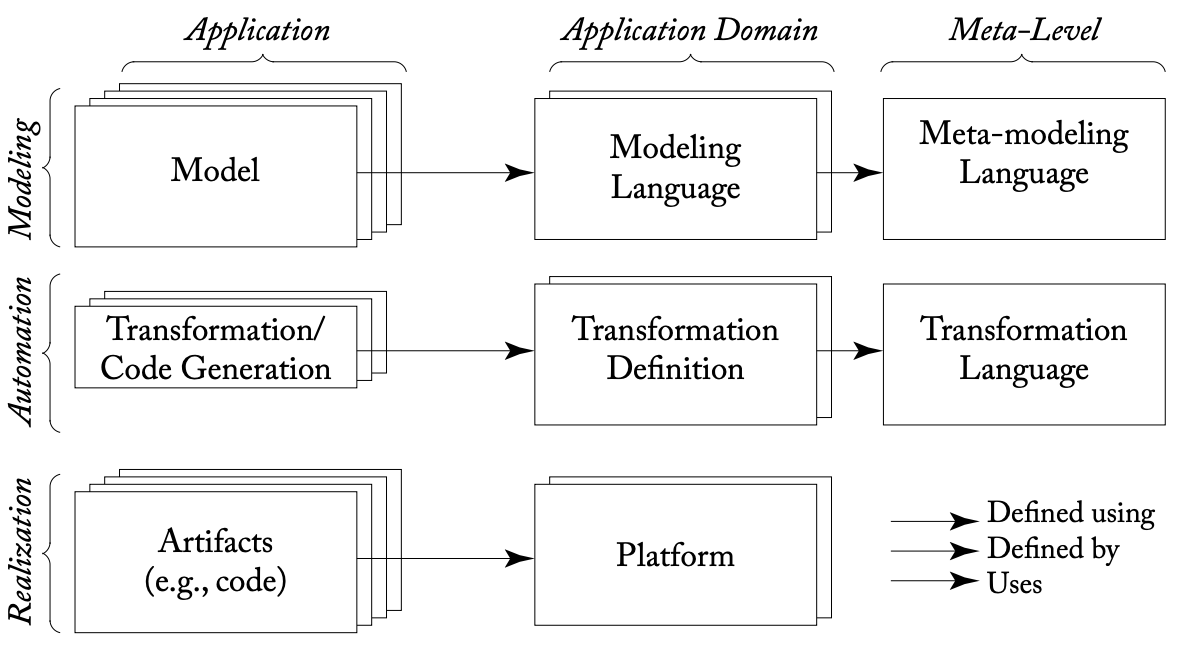
\includegraphics[width=.8\columnwidth]{mdse.png}
	\caption{Test-Driven process to repair models}
	\label{fig:mdse}
\end{figure}

There is a literature on how to design high quality models \cite{Krogstie:2012:MDE:2331118}, however keeping all the different models conformant while code-base evolves, is one of the main challenges in model-based software engineering.
The model repair approaches proposed in this thesis try to improve the state of the art for model repair, by giving more tools or methods for software engineers to apply in the industrial practice, or to further extend.

%\subsection{Models in the Software Development Lifecycle}
%to copy from various sources, including the MDE book by Krogstie.

%\subsection{Model Transformations}
%M2M, M2T, T2M, T2T transformations (copy from MDE book)

%\section{Software Artifacts}\label{sec:models}

Whereas with the recent advent of agile methodologies, such as the scrum development process, the usage of models is sometimes interpreted as being discouraged, empirical evidence shows that a trade-off on which models to keep, should be found \cite{blasband2016rise}. As code evolves, models should be updated too to maintain conformance with code, and this operations take time: therefore which models to keep and which not, should be a careful decision to make \cite{blasband2016rise}.
Indeed, models have the positive effect of being more easily understandable than code and, among their functions, models are particularly important in helping engineers to transfer domain knowledge, and collaborate with others.
A trade-off should be found, but models remain covering an important function in the software development process, therefore all the model-driven engineering activities are of importance.

In the rest of the section, we describe the three model types that we chose as target for the repair operations identified in this thesis: combinatorial contraints, feature models, and timed automata.

\subsection{Combinatorial Constraints}

Combinatorial Interaction Testing (CIT), or simply combinatorial testing, aims to test the software or the system with selected combinations of parameter values. 
There exist several tools and techniques for CIT. Good surveys of ongoing research in CIT can be found in~\cite{GrindalSTVR05,NieL11}, while an introduction to CIT and its efficacy in practice can be found in~\cite{kuhncomputer09,Petke15:practical}. 

A model for a combinatorial problem consists of several parameters %(at least 2) 
which can take several domain values. 
In most configurable systems, dependencies exist between parameters. 
Such constraints may be introduced for several reasons, e.g., to model inconsistencies between certain hardware components, limitations of the possible system configurations, or simply design choices~\cite{CohenTSE08}. 
In our approach, tests that do not satisfy the constraints in the CIT model are considered \emph{invalid}.

CIT problems can be formally defined as follows.

\begin{defn}
	Let $P=\{p_{1},\dots,p_{m}\}$ be the
	set of parameters. Every parameter $p_{i}$ assumes values in the domain $D_{i}=\{v_{1}^{i},\ldots,v_{o_{i}}^{i}\}$. 
	Every parameter has its name (it can have also a type with its own name) and every enumerative value has an explicit name. We denote with $C=\{c_{1},\ldots,c_{n}\}$
	the set of constraints.
\end{defn}

%\begin{defn}
%	The objective of a CIT test suite is to cover all parameter interactions between any set of $t$ parameters. $t$ is called the strength of the CIT test suite. For example, a pairwise test suite covers all combinations of values between any 2 parameters.
%\end{defn}

Constraints $c_i$ are given in general form, using the language of propositional logic with equality and arithmetic. 
%Fig.~\ref{fig:washerexample} shows the \citlab{} model of a simple washing machine consisting of 3 parameters. The user can select if the machine has \texttt{HalfLoad}, the desired \texttt{Rinse}, and the \texttt{Spin} cycle speed.
%There are two constraints, including,  if \texttt{HalfLoad} is set then the speed of spin cycle cannot exceed \texttt{maxSpinHL}.

Software systems can be configured by setting specific parameter values at different stages of the software testing process.

\noindent {\bf Compile time}
Configurations can be set at compile time. An example is shown in Figure~\ref{fig:compiletimeConf}. Depending on the value settings of the Boolean variables \texttt{HELLO} and \texttt{BYE} different messages will be displayed when the program is run.

\noindent {\bf Design time}
Configurations can also be set at design time. For example, in case of a SPL, a configurability model is built during the design. 

%\item 
\noindent {\bf Runtime}
%\red{something that one can customize at run time via conf file}
Another way of setting parameter configurations is at runtime. This can be usually done by means of a graphical user interface (GUI). In a chat client, e.g., you can change your availability status as the program is running. 

\noindent {\bf Launch time}
We also differentiate the case where parameters are read from a separate configuration file or given as program arguments, \emph{before} the system is run. We say that these parameters are set at launch time of the given application. They decide which features of the system should be activated at startup. Examples of such systems include chat clients, web browsers and others. 

\begin{comment}
\todo{cite from constraintsrepair}
A model for a combinatorial problem consists of several parameters (at least 2) which can take various domain values. 
In most configurable systems, constraints (or dependencies) exist between parameters. 

Constraints might be introduced for several
reasons, for example, to model inconsistencies between certain hardware
components, limitations of the possible system configurations, or
simply because of design choices~\cite{CohenISSTA07}. Constraints were first
described as being important to combinatorial testing in~\cite{AETG}
and were introduced in the AETG system. In our approach tests that
do not satisfy the constraints in the CIT model are considered \emph{invalid}.

In classical combinatorial interaction testing, only valid tests are generated, since the focus is on assessing if the system under test produces valid outputs. 
%testing the software implementation. 
However, we believe that invalid tests are also useful.  In particular, a combinatorial model can be overconstrained, that is, it might restrict generation of test cases that are valid in the system, yet not be generated due to the constraints in the given model. Furthermore, critical safety systems should be tested if they failed safely in case an invalid configuration is entered. Moreover, creation of a CIT model for a large real-world software system is usually a tedious, error-prone task. Therefore, invalid configurations generated by the model at hand can help reveal constraints within the system under test and help refine the combinatorial model.
\end{comment}


\subsection{Feature Models}
%// TODO change because copied from Oster's PhD thesis introduction
Software Product Line (SPL) engineering is an approach for the systematic reuse of software artifacts across a very large number of similar products. 
Various domains apply SPL engineering successfully to improve the overall project success, by increasing quality, saving costs for development and maintenance, and decreasing time-to-market \cite{bookSPL2001}. 
SPLs offer a systematic reuse of software artifacts within a range of products sharing a common set of features (i.e., units of functionality) \cite{Griss2000}.
According to IEEE a feature is a distinguishing characteristic of a software item (e.g. concerning its performance, portability, or functionality) \cite{ieeeterminology}.

The central aspect of systematic reuse is the concept of variability. This concept provides the possibility to define particular artifacts (features) for the entire SPL as not necessarily being part of each product. Variability specifies the point at which features are selected in combination with other features \cite{CE00}. The stakeholders of the SPL generally define where variability occurs and decide which features are variable e.g. optional or alternate.
% Variability leads to a combinatorial explosion of possible products from one SPL. % For instance, an SPL with around 200 optional features may lead to over 1060 different products.

Feature models represent variability in software product lines, and are employed in various domains, in particular in the IoT and in the automotive sector.
However, variability model repair, in the context of systematic variability management in software, is still challenging and a relatively new problem.
One main reason for the increasing need of systematic variability management in software is the fact that the majority of modern features in a car are based on software. Thus, variability moves from mechanics and hardware to software \cite{bosch_spl_nokia,oster_feature_2011}.

%The concept of Product Lines is not new and engineers in various domains, such as the automotive sector, have adopted this concept of development for the last few decades, to benefit from the advantages that SPL engineering offers. However, with regard to software, systematic reuse, including variability concepts, is still challenging and a relatively new problem for the automotive sector. One main reason for the increasing need of systematic variability management in software is the fact that the majority of modern features in a car are based on software. Thus, variability moves from mechanics and hardware to software \cite{bosch_spl_nokia}.

%Due to variability, we are increasingly encountering a situation in the automotive sector where a single electronic control unit (ECU) may be instantiated in at least 10,000 different ways, and the software running on a network of more than 50 ECUs in a single car may exist in millions of different configurations. As a result, we are confronted with a world where any instance of a certain brand of car possesses a unique configuration of the embedded software of all its ECUs. At a first glance, this situation seems to result in a major benefit for the automotive sector and other industrial domains, allowing the combination of mass customization and the ability to produce individual, customer-specific configurations.

\subsection{Timed Automata}

Timed automata is proposed by Alur and Dill \cite{AD94} in the early nineties as an extension to the classical automata, which is extended with clock variables. 
Timed automata theory has become an important research area and been widely studied in the context of both formal languages and verification of real time systems \cite{5521565}.

One main application of timed automata is the verification of properties using model checking methods \cite{clarke_model_checking}, by traversing through all reachable states.
Another application is robustness analysis of systems that can be modeled by a TA \cite{markey2011robustness}.

Timed automata have academic and industrial applications for the modeling and verification of protocols: such as TDMA (Time Division Multiple Access) protocol \cite{tdma}, power controller protocols \cite{havelund_power_controller_1999}, and security protocols such as Kerberos, TMN, Neumann Stubblebine, Andrew Secure and Wide Mouthed Frog \cite{jakubowska2005verifying,jakubowska2007modelling}.

Timed automata are equipped with of clock variables that record the passage of time since they have been reset. All clocks are synchronized and they run at the same speed. 
The transitions from one state to another are assumed to be instantaneous; in other words, time passes only in states, not on edges.

An example of time automaton is given in Fig. \ref{figure:example-TA}.%\todo{figura}

A formal definition of timed automata is given in Sect. \ref{sec:definitions1}.

\subsection{Model Repair and Program Repair}
To the best of our knowledge, few studies address the problem of repairing the \textit{model} artifacts, instead of the implementation code, and the problem of repair \textit{automatically} existing models of software systems w.r.t. the implementation is still an open issue. 
There are, however, several works on automated repair of programs \cite{Nguyen_2013,le_goues_systematic_2012,ARCURI20113494}.
In model-driven engineering, there are approaches aiming at repairing inconsistencies between models \cite{Macedo_2013}; Tran et al. show a way to address the problem \textit{manually} for the Linux Kernel \cite{Tran:1999:FRR:781995.782007}; Nadi et al. present a method to automatically \textit{mine} conditions under which a system behaves in a certain way \cite{NadiBKC14}, and there are methods to statistically infer constraints from data~\cite{chiang_unified_2011,Abukwaik_2016}, but they are not directly applicable to repair existing models made of sets of constraints and they do not guarantee complete accuracy. 
A quality-based model refactoring framework assessing quality of merging operations among SPL models, expressed in UML~\cite{rubin_quality_2013}, supports maintainability of models describing relations among features. It represents an approach to model repair, although it is specific to one kind of models.
The need of a fault-driven constraint repair process was already envisioned in~\cite{henard_towards_2013}, but any empirical experiment were yet performed.


\section{Software Testing for Model Repair}\label{sec:testing}
Software systems are an integral part of life, from business applications (e.g., banking) to consumer
products (e.g., cars). Most people have had an experience with software that did not work as expected.
Software that does not work correctly can lead to many problems, including loss of money, time, or
business reputation, and even injury or death. Software testing is a way to assess the quality of the
software and to reduce the risk of software failure in operation.

Software testing is expensive and labor intensive. Software testing requires up to 50\% of software development costs, and even more for safety-critical applications \cite{testingbook}.

Therefore, software testing has been an active area both in research and in industry.
There are several studies and techniques to adapt software testing to specific scenarios and applications, to improve test suite generation and execution, and to apply testing techniques to various tasks in software engineering, such as program repair and model inference and repair. \cite{le_goues_systematic_2012,chiang_unified_2011,Duchene:2012,Xuan_2017}

One of the goals of software testing is to automate as much as possible, thereby significantly reducing its cost, minimizing human error, and making regression testing easier. \cite{testingbook}

\subsection{Combinatorial Testing}
Combinatorial Interaction Testing (CIT) aims at covering the interactions of parameters in a system under test (SUT), while some combinations may be forbidden by given constraints (forbidden tuples) \cite{yamada_greedy_2016}.
It explores t-way feature interactions inside a given system, by effectively combining all t-tuples of parameter assignments in the smallest possible number of test cases.
This allows to budget-constrain the costs of testing while still having a testing process driven by an effective and exhaustive coverage metric \cite{AETG,KuhnTSE04}. 
The most commonly applied combinatorial testing technique is pairwise testing, which consists in applying the smallest possible test suite covering all pairs of input values (each pair in at least one test case). 
In fact, it has been experimentally shown that a test suite covering just all pairs of input values can already detect a significantly large part (typically 50\% to 75\%) of the faults in a program \cite{Dalal:ICSE99, IPO}.
Dunietz et al. \cite{Dunietz:ICSE97} compared t-wise coverage to random input testing with respect to the percentage of structural (block) coverage achieved, showing that the former achieves better results if compared to random test suites of the same size. 
Burr and Young \cite{burr98} reported 93\% code coverage from applying pairwise testing of a large commercial software system, and many CIT tools (see \cite{pairwise} for an up to date listing) and techniques have already been developed \cite{Dalal1998a,GrindalSTVR05,KuhnTSE04} and are currently applied in practice \cite{Brownlie1992a,Kuhn02,Smith}. 
CIT is used in a variety of applications for unit, system, and interoperability testing. 
It has generated both high-level test plans and detailed test cases. In several applications, it greatly reduced the cost of test plan development. Testers can base their input on detailed development requirements or on a system's high-level functional requirements.

\subsection{The Oracle Problem}

In software testing, while test case generation, execution and fault localization have considerably advanced, the quality of the oracle remains an important bottleneck \cite{jahangirova_empirical_2019}.

The effectiveness of testing depends both on the quality of the test cases and on the quality of the oracle \cite{barr_oracle_2015,staats_programs_2011,weyuker_testing_1982}. 
The Oracle Problem is the problem of defining accurate oracles, capable of detecting all and only faulty behaviours exercised during testing [12], [18], [25], [36], [37], [38]. Without a (good) oracle to determine whether the test output is correct, test inputs that satisfy the strictest adequacy criteria remain useless and testing is ineffective.
The quality of the oracle can be evaluated based on two properties: \textit{completeness} (no false positives), and soundness (no false negatives: all faults should be rejected by the oracle).

%Oracle assessment must thus identify and report false positives or false negatives (or both), so as to support the developer in improving the oracle soundness and completeness.


%TODO to copy from Tonella e Jahangirova papers...
With respect to our proposed model repair process, we assume the existence of an oracle to assess non-conformancies between the model and the system.
In one case we automated the oracle (we used the implicit oracle), in other cases, the oracle could be set by the user or predicted.
Oracle evaluation is often the longest phase in software testing, and a bottleneck in testing automation. Indeed, it is where domain knowledge expertise is needed, and often only human intervention is reliable, as the oracle is intimately related to domain knowledge representation, and to requirements engineering.

%\section{Manipulation Techniques}
\subsection{SAT and SMT solvers}

In computer science, the Boolean satisfiability problem (sometimes called propositional satisfiability problem and abbreviated SATISFIABILITY or SAT) is the problem of determining if there exists an interpretation that satisfies a given Boolean formula. 
In other words, it asks whether the variables of a given Boolean formula can be consistently replaced by the values TRUE or FALSE in such a way that the formula evaluates to TRUE. If this is the case, the formula is called satisfiable. On the other hand, if no such assignment exists, the function expressed by the formula is FALSE for all possible variable assignments and the formula is unsatisfiable. For example, the formula "a AND NOT b" is satisfiable because one can find the values a = TRUE and b = FALSE, which make (a AND NOT b) = TRUE. In contrast, "a AND NOT a" is unsatisfiable.

SAT is the first problem that was proven to be NP-complete.
Nevertheless, as of 2007, heuristic SAT-algorithms are able to solve problem instances involving tens of thousands of variables and formulas consisting of millions of symbols, which is sufficient for many practical SAT problems from, e.g., artificial intelligence, circuit design, and automatic theorem proving.

SAT and SMT solvers are employed in various applications in software engineering, especially in model checking, program verification, and static analysis \cite{sat2008}.
In presence of constraints in propositional logic, they allow to determine if a particular assignment of values to parameters is satisfiable or not. It is related to the oracle problem. These techniques are also used to identify redundant constraints, and for constraints simplification. They also allow to obtain failure-inducing combinations between two sets of constraints.

By definition, the SAT problem takes as input a propositional formula in Conjunctive Normal Form (CNF), normally as DIMACS format, and a variable assignment, and tells whether it is satisfiable or not.

Although the SAT solver is very fast, transforming a propositional formula in an arbitrary format into CNF, although always possible, can be computationally expensive, and lead to an exponential grow in formula size.

This is one of the practical reasons why for some applications in software engineering, BDDs are preferred over SAT/SMT solvers.

%\subsection{Search-based Software Engineering}
%\subsection{Model Checkers}

\subsection{BDDs and MDDs}

Binary Decision Diagrams (BDD) and Multi-Valued Decisions Diagrams (MDD) are commonly used structures for representing Boolean functions and multi-valued functions, respectively. 

%A binary decision diagram (BDD) or branching program is a data structure that is used to represent a Boolean function. 
On a more abstract level, BDDs can be considered as a compressed representation of sets or relations. Unlike other compressed representations, operations are performed directly on the compressed representation, i.e. without decompression. Other data structures used to represent Boolean functions include negation normal form (NNF), Zhegalkin polynomials, and propositional directed acyclic graphs (PDAG).

BDDs are extensively used in CAD software to synthesize circuits (logic synthesis) and in formal verification. There are several lesser known applications of BDD, including fault tree analysis, Bayesian reasoning, product configuration, and private information retrieval.

Although building a BDD is normally computationally more expensive than solving a SAT problem with a state-of-the-art SAT solver, it allows for a deeper analysis over the propositional formula that leads to the BDD, in particular:
\begin{itemize}
	\item Using the BDD representation, it is easy to count the number of satisfiable configurations. This may be useful in certain contexts such when this number is a part of a fitness function of a process, or is needed for evaluation.
	\item BDDs do not need the input formula (or set of constraints) to be in a CNF representation, therefore avoiding the potentially exponential complexity of the CNF transformation.
	\item BDDs can be more convenient, and potentially faster, when multiple assignments are to be evaluated over the same propositional formula, because the tree is built only once (building the BDD is the complex operation), and then just traversed many times to check for satisfiability.
\end{itemize} 


\part{Test-Driven Model Repair Approaches}
\chapter{Automated Model Repair}\label{ch:automatedrepair}
We devise an iterative process to automatically repair models: the model is modified until all the non-conformances between the model and the system (revealed by the generated tests), are solved. Fig. \ref{fig:researchapproach} shows an overview of such test-driven repair approach. 
Among testing techniques to be employed, black-box testing is an effective technique to detect faults in a system focusing on the inputs, without needing access to the code, but requiring simply an oracle that states if a particular test passes or fails. 
Combinatorial Interaction Testing (CIT), in particular, has shown to achieve high coverage in software systems for which a parametric, configurable model can be defined. Moreover, we use mutation analysis and search-based methods for \textit{feature models}, a model that has also a graphical tree representation, and these methods tend to apply \textit{small} edits to the model, helping preserve domain knowledge.

Unlike processes that detect faults and repair code, the main hypothesis of this project is that testing techniques can be used not only for fault detection and localization, but also for model repair.
This methodology aims at changing the model \textit{with less impact as possible} (to preserve domain knowledge) to \textit{repair} the non-conformance w.r.t. the \textit{solution space} (it can be the current implementation, a new specification, or an available \textit{oracle}).
The applied repairs are local and little, based on the \textit{competent modeler} assumption, that the model is \textit{a little} outdated, and minimal changes are enough. 


\section{Research Hypothesis}
\begin{tikzborder}{\cite{radavelli2019using}}
By making the assumption that the fault resides in the model, and the implementation is correct, the rationale that drives this PhD proposal is the investigation of software testing techniques to automatically \textit{repair} models.
Model \textit{repair} can be useful whenever the model is outdated w.r.t. the implementation, or a defined oracle or the specification.
Sometimes an engineer also wants to detect which is a model of a current aspect of an implemented system, and can use testing techniques not only to find bugs in a system, but also to \textit{repair} or to entirely \textit{learn} a model from the system implementation.

The main hypothesis of this research project is that testing techniques can be used not only for fault detection and localization, but also for model repair.
\be

\subsection{Assumptions}
The applicability of the proposed failure-driven model repair framework is subject to the following assumptions, that we identified:
\begin{itemize}
	\item prescriptive model: there should be an initial prescriptive model of the system, from which tests can be then generated;
	\item traceability: the parameters in the model can be traced back to variable in the system. It should be always possible to translate an abstract configuration (i.e., a test), into a concrete test;
	\item oracle definition: there should be the possibility to execute a test towards the system, and obtain a \textit{pass}/\textit{fail} result, e.g., depending if the system compiles correctly, doesn't crash, doesn't expose a vulnerability, etc.
	\item faulty model: we assume that the fault(s), if present, reside in the model, while the system is correct, and can be used as oracle.
\end{itemize}

\section{Contribution}\label{sec:contribution}
\bb
The contribution of this PhD project is the proposal and evaluation of testing techniques to repair models of software systems.
The methodology aims at changing the model \textit{with less impact as possible} (to preserve domain knowledge) to \textit{repair} the non-conformance w.r.t. the \textit{solution space} (it can be the current implementation, a new specification, or an available \textit{oracle}).
\be

From the initial prescriptive model, (1) we generate and execute tests (test generation), (2) we detect failing interactions (fault localization), and (3) we repair the model accordingly (model repair), obtaining a \textit{descriptive} model of the system, that we assume to \textit{accurately} represent the new \textit{prescriptive} model of the system.

%\bb In the rest of this PhD proposal, we present the research methodology, and the already evaluated application in the scenarios of (1) combinatorial models, and (2) feature models in software product line enginnering.
%We then discuss other possible scenarios in which model repair can be employed. \be

\section{Research Approach}\label{sec:researchapproach}
\bb
The research process, designed in accordance with the defined objectives, consists of two stages: the reviewing stage, and the formulation stage.
In the reviewing stage, we evaluate existing techniques that may be useful for the objective, and explore possible application scenarios, to determine the kind of models that can be repaired from software testing results.
In the formulation stage, for each scenario, we try to formulate the concepts and \textit{decline} the repair problem to that particular kind of model; then we apply or tailor the existing techniques to propose a solution to the model repair problem.
Among testing techniques to be employed, black-box testing is an effective technique to detect faults in a system focusing on the inputs, without needing access to the code, but requiring simply an oracle that states if a particular test %(i.e., a system configuration)
passes or fails. 
Combinatorial Interaction Testing (CIT), in particular, has shown to achieve high coverage in software systems for which a parametric, configurable model can be defined. Mutation analysis and search-based methods are also to take into consideration, when possible, as they tend to apply \textit{small} edits to the model, helping preserve domain knowledge.
The process is iterative: the model is modified until all the non-conformances between the model and the system (revealed by the generated tests), are solved. Fig. \ref{fig:researchapproach} shows an overview of such test-driven repair process. 
Benchmarks should be selected for evaluation, and tools to implement the repair process should be reused if existing, or customized or built if needed.%; customization or optimization of existing algorithms could also be performed.
\be

\begin{figure}[!htb]
	\centering
	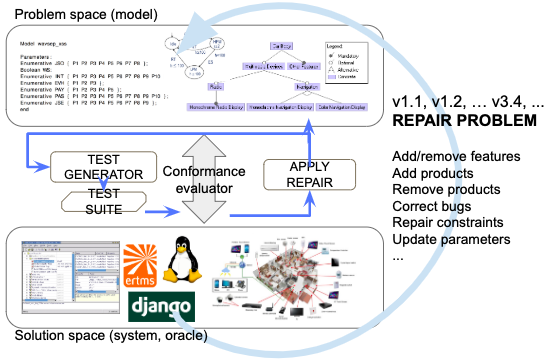
\includegraphics[width=.8\columnwidth]{images/repair.png}
	\caption{Test-Driven process to repair models}
	\label{fig:researchapproach}
\end{figure}

\section{Results to date}
\bb
In the initial stage of the research project we applied the repair process to \textit{configurable} models.
Configurable models can model, for example, system features decided at \textit{compile time} such as preprocessor directives, or decided at \textit{operation time} such as configuration files, and also constraints among parameters in a running system.

In the following subsections we briefly describe the results obtained from the application of test-driven repair in two kinds of configurable models: combinatorial models and feature models.
\be

\subsection{Repair of Configuration Constraints}\label{sec:constraintrepair}

\bb
A model for a combinatorial problem consists of parameters which can take various domain values. Combinatorial models may have also constraints among parameter values to, for example, model inconsistencies between certain hardware components, limitations of the possible system configurations, or simply because of design choices.
%We devise an approach in which tests that do not satisfy the constraints in the CIT model are considered invalid.
Some methods have been introduced to automate the process of inferring constraints, but they do not aim at \textit{repairing} existing ones \cite{Abukwaik_2016,Temple16:using}. 
Therefore, in \cite{gargantini_combinatorial_2017} %, to find and fix conformance faults between the given software system and its combinatorial model, 
we proposed an iterative approach that uses a fault-localization tool based on combinatorial testing, called BEN, and CIT policies introduced in our previous work \cite{Gargantini16:validation} to find failure-inducing combinations of parameter values.
The model is then repaired \textit{logically}, by translating such failure-inducing combinations as expression in propositional logic.
We also developed a tool to make it easier the editing of such combinatorial models, and the test suite generation, called CTWedge \cite{IWCTGargantini2018}.
%We also developed a tool to edit such combinatorial models, and generate tests, called CTWedge \cite{IWCTGargantini2018}.
\be

Chapter \ref{ch:constraintrepair} presents results in detail.

\subsection{Repair of Feature Models}\label{sec:fmrepair}

\bb
Feature models are a widely used modeling notation for variability management in software product line (SPL) engineering. 
In order to keep an SPL and its feature model aligned, feature models must be changed by including/excluding new features and products, either because faults in the model are found or to reflect the normal evolution of the SPL.
Such changes can be complex and error-prone due to the size of the feature model.
%The modification of the feature model to be made to satisfy these change requirements can be complex and error-prone. 
%In this case study, w
Therefore, we try to \textit{repair} a feature model w.r.t. a given update request in the form of a set of configurations to be accepted or rejected, that may come from \textit{failing} test cases, or from a change in the specification.
The method is based on an evolutionary algorithm that iteratively mutates the original feature models and checks if the update request is semantically fulfilled \cite{arcaini_evolutionary_2018,arcaini2019achieving}. %, by using BDDs. %The process terminates until the model is completely updated or some other termination condition occurs.
%Among all the possible models achieving the update request, the method privileges those structurally simpler, to preserve domain knowledge.
The approach has been evaluated on real-world feature models: although it does not guarantee to completely update all the possible feature models, on average, around 89\% of requested changes are applied, %and since the process is based on small mutations, 
with minimal edits, helping in preserving domain knowledge.% from previous models.
\be

Chapter \ref{ch:fmrepair} presents results in detail.

\subsection{Repair of Timed Automata}
We apply the repair framework also to timed automata clock guards. In this case, a test is a timed sequence (i.e., actions associated to an absolute time) that can be exercised on the real system.
Our approach generates an abstraction of the initial TA in terms of a PTA, generates some tests, and then refines the abstraction by identifying only those TAs contained in the PTA that correctly evaluate all the tests. 
Chapter \ref{ch:tarepair} presents results in detail.

\chapter{Repair of Feature Models}\label{ch:fmrepair}

Feature are a widely used modeling notation for variability management in software product line (SPL) engineering. 
The goal of this chapter is to propose an answer to the research question RQ3 introduced in Sect. \ref{sec:intro}: "How to repair feature models?".
We present two different techniques to repair feature models.
The first approach allows to repair feature models represented in the hierarchical tree-like structure, as well as \textit{simple} constraints (i.e., only in the form of \textit{requires} and \textit{excludes} between couple of features) in propositional logic.
The second approach, instead, applies to feature models represented as arbitrarily \textit{complex} constraints, expressed in propositional logic.
The two approaches can be combined, as to fully represent variability, unless complicating the model with a large number of abstract feature, it is normally more convenient to use \textit{general} (i.e., \textit{complex}) constraints, besides the hierarchical tree-like structure of feature dependencies.
In the rest of the chapter, Sect. \ref{sec:fm1} covers the first approach reporting from paper \cite{arcaini2019achieving}, which includes and extends the previous paper \cite{arcaini_evolutionary_2018}.

Related work for the two approaches are discussed jointly in Sect. \ref{sec:fmrelated} , and Sect. \ref{sec:fmconclusion} concludes the chapter.


\section{Achieving change requirements of feature models by an evolutionary approach}\label{sec:fm1}
We developed an approach that \textit{repairs} a feature model w.r.t. a given update request in the form of combinations representing a set of configurations to be accepted or rejected, that may be detected by \textit{failing} test cases, or directly by engineer domain knowledge. % from a change in the specification.
The method is based on an evolutionary algorithm that iteratively mutates the original feature models and checks if the update request is semantically fulfilled.
We employ mutations such as switching an optional feature to mandatory, or changing an \emph{or} group to an \emph{and} group, based on \cite{arcaini_evolutionary_2018}.
We generate faults between two real versions of feature models of the {\tt MobileMedia}, {\tt HelpSystem},  {\tt SmartHome}, and {\tt ERP\_SPL} systems in the SPLOT repository\footnote{\url{http://52.32.1.180:8080/SPLOT/feature_model_repository.html}}, and we notice that although our approach does not guarantee to completely update all the possible feature models, on average, around 89\% of requested changes are applied, with minimal edits.%, helping in preserving domain knowledge.

\subsection{Basic definitions}\label{sec:basicDef}

\begin{tikzborder}{\cite{arcaini_evolutionary_2018}}
In software product line engineering, feature models are a special type of information model representing all possible products of an SPL in terms of features and relations among them. Specifically, a feature model \fm is a hierarchically arranged set of features $F$, where each parent-child relation between them is a constraint of one of the following types\footnote{As done by FeatureIDE~\cite{FeatureIDEbook}, we assume that each feature can be the father of only one group (either {\it Or}, {\it Alternative}, or {\it And}). This is not a limitation, as having different groups as children can be obtained by using abstract features~\cite{thum_abstract_2011}.}:
%
\begin{compactitem}
\item \textit{Or}: at least one of the sub-features must be selected if the parent is selected.
\item \textit{Alternative} (xor): exactly one of the children must be selected whenever the parent feature is selected.
\item \textit{And}: if the relation between a feature and its children is neither an \textit{Or} nor an \textit{Alternative}, it is called \textit{and}. Each child of an \textit{and} must be either:
\begin{compactitem}
\item \textit{Mandatory}: the child feature is selected whenever its respective parent feature is selected.
\item \textit{Optional}: the child feature may or may not be selected if its parent feature is selected.
\end{compactitem}
\end{compactitem}

Only one feature in $F$ has no parent and it is the \emph{root} of \fm.

In addition to the parental relations, it is possible to add \emph{cross-tree constraints}, i.e., relations that cross-cut hierarchy dependencies. {\it Simple} cross-tree constraints are:
%
\begin{compactitem}
\item A {\it requires} B: the selection of feature A in a product implies the selection of feature B. We also indicate it as $A \rightarrow B$.
\item A {\it excludes} B: A and B cannot be part of the same product. We also indicate it as $A \rightarrow \neg B$.
\end{compactitem}

Some frameworks for feature models also support {\it complex} cross-tree constraints~\cite{knuppel_is_2017} through \textit{general} propositional formulas. In our approach, we allow feature models to contain complex cross-tree constraints.

Feature models can be visually represented by means of feature diagrams, and their semantics can be expressed by using propositional logic~\cite{batory2005feature,benavides2010automated}: features are represented by propositional variables, and relations among features by propositional formulae. We identify with $\fmToBool(\fm)$ the \textsc{BO}olean \textsc{F}ormula representing a feature model \fm.

\begin{mydef}[\textbf{Configuration}]\label{def:configuration1}
A \emph{configuration} $c$ of a feature model \fm is a subset of the features $F$ of \fm (i.e., $c \subseteq F$).
\end{mydef}

If \fm has $n$ features, there are $2^n$ possible configurations.

\begin{mydef}[\textbf{Validity}]\label{def:validity}
Given a feature model \fm, a configuration $c$ is \emph{valid} if it contains the \emph{root} and respects the constraints of \fm. A valid configuration is called \emph{product}.
\end{mydef}

For our purposes, we exploit the propositional representation of feature models for giving an alternative definition of configuration as a set of $n$ literals $c = \{l_1, \ldots, l_n\}$ (with $n = |F|$), where a positive literal $l_i=f_i$ means that feature $f_i$ belongs to the configuration, while a negative literal $l_i=\neg f_i$ means that $f_i$ does not belong to the configuration. We will also represent a configuration as a BOolean Formula as follows: $\fmToBool(c) = \bigwedge_{i=1}^n l_i$.

Furthermore, since in the proposed approach we need to evaluate a feature model over a possibly wider set of features $U$, we introduce $\fmToBool(\fm, U) = \fmToBool(\fm) \wedge \bigwedge_{f \in U \setminus F} \neg f$, where \fm explicitly refuses all the configurations containing a feature not belonging to its set of features $F$; such technique has been already employed by different approaches that need to compare feature models defined over different sets of features~\cite{thum_reasoning_2009,icst2015}.
\be

\begin{exmp}\label{ex:initialFM}
\bb
Let's consider the feature model shown in Fig.~\ref{fig:fmExample}.
\be
%
\begin{figure}[!htb]
\centering
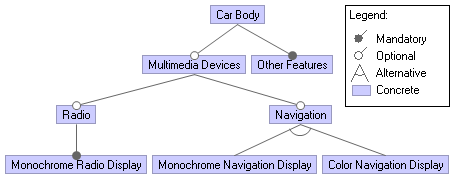
\includegraphics[height=3.5cm]{car2011}
\caption{Example of feature model (taken from~\cite{Pleuss2012})}
\label{fig:fmExample}
\end{figure}
%
\bb
It is the third version of the CAR SPL described in~\cite{Pleuss2012}. It is composed of eight features $F$ = \{\CarBody, \MultimediaDevices, \OtherFeatures, \Radio, \Navigation, \MonochromeRadioDisplay, \MonochromeNavigationDisplay, \ColorNavigationDisplay{}\}. \CarBody is the root feature; its children \MultimediaDevices and \OtherFeatures are respectively optional and mandatory. \MultimediaDevices has two optional children: \Radio that is the father of the mandatory feature \MonochromeRadioDisplay, and \Navigation that is the father of the alternative group between \MonochromeNavigationDisplay and \ColorNavigationDisplay.\be
\end{exmp}

\subsection{Specifying an update request}\label{sec:updateRequest}

\bb We suppose that the product line engineer wants to update an existing feature model \initFm ({\it initial feature model}); although (s)he knows which are the desired updates in terms of products and features to add or remove, (s)he does not know how to write a feature model \fmp that satisfies all these updates.

In this section, we describe how the user can specify her/his {\it change requirements}.
By analysing existing evolutions of feature models described in literature~\cite{Pleuss2012,Burdek2016,smartHomePaper,helpSystemPaper,multimediaPaper}, we identified the following five types of change requirements: 
%
\begin{compactitem}
\item a feature must be identified with a new name. Although this change requirement is straightforward to achieve, it is widely used (e.g., for the Smart\-Home SPL~\cite{smartHomePaper} considered in the Ample Project, we have observed 12 feature renames) and it is important to keep track of it, otherwise someone reading the updated feature model may have the impression that one feature has been added and one removed (in particular, if also other changes have been done on the feature model and, therefore, spotting the renamed feature is not easy).
\item a feature must be added to the feature model. This change requirement occurs when a new feature must now be supported by the SPL. For example, in the CAR SPL~\cite{Pleuss2012}, the support for {\it DVD entertainment} has been introduced in 2012 (documented in the fourth version of the SPL feature model).
\item a feature must be removed from the feature model. This change requirement occurs when a feature is no more supported by the SPL.\footnote{Note that this change requirement could be achieved by removing all the products containing the feature (see last change requirement), but not removing the feature from the feature model. However, in this way, the feature would become {\it dead}~\cite{benavides2010automated}, making the feature model less readable.} For example, in the CAR SPL~\cite{Pleuss2012}, feature {\it Color Radio Display} has been removed in 2011 (third version of the SPL feature model).
\item some products must now be accepted by the SPL. This change requirement occurs when some constraints existing on the SPL (due to technical reasons or regulations) do not hold anymore and so some configurations that were forbidden in the past can now be accepted. For example, in the second version of the Pick-\&-Place (PPU) Unit SPL~\cite{Burdek2016}, the system is able to process either {\it plastic} or {\it metal} workpieces; in the third version of the SPL, instead, a technical improvement has allowed to handle plastic and metal workpieces in combination.
\item some products cannot be accepted anymore by the SPL. This change requirement happens when some constraints over the SPL emerge (e.g., due to new regulations). For example, in the {HelpSystem} SPL~\cite{helpSystemPaper}, the second version of the SPL does not allow anymore that the sensor only detects either {\it pressure} or {\it not pressure}, i.e., the products with only {\it pressure} or {\it not pressure} are not allowed and have been removed.
\end{compactitem}

In the following, we provide the formal definition of update request. We assume that the initial feature model does not contain any dead feature or redundant constraint~\cite{benavides2010automated,Duran2017FLAME}; in case it has any, we can remove them using standard techniques, as, for example, that provided by FeatureIDE~\cite{FeatureIDEbook}.

\begin{mydef}[\textbf{Update request}]\label{def:fic1}
Given an initial feature model \initFm defined over a set of features $F$, we call \emph{update request} \UR the modifications a user wants to apply to \initFm in order to obtain the desired updated model \fmp. An update request is composed of five change requirements, three regarding the features of the feature model, and two the configurations/products. The first \emph{feature-based} change requirement regards the features names:
%
\begin{compactitem}
\item {\bf Rename features}: $\Ftbr = \{f_1,$ $\ldots,$ $f_m\}$ is a subset of features of $F$ that must be renamed and \rename a renaming function; \renamedFeatures is the set obtained by replacing every feature $f_i \in \Ftbr$ with $\mathit{ren}(f_i)$, i.e., $\renamedFeatures = (F \setminus \Ftbr) \cup \bigcup_{f_i \in \Ftbr} \{\rename(f_i)\}$. We identify with \fmrenamed the feature model obtained by renaming the features according to \Ftbr and \rename.\footnote{Note that feature renaming is already supported by feature model editors, such as FeatureIDE. We keep it among our change requirements for completeness with respect to the feature model evolutions observed in literature.}
\end{compactitem}
The other two \emph{feature-based} change requirements over the features of \fmrenamed are:
\begin{compactitem}
\item {\bf Add features}: \Fadd is a set of features the user wants to add to \fmrenamed. For each $e$ in \Fadd, the user has to define in $F_R \cup \Fadd$ the parent of $e$, denoted by \parent{e}. By adding a feature $e$ with parent $p$, we assume that the user wants to duplicate all the products that contain $p$ by adding also $e$.\footnote{Note that this corresponds to have $e$ as optional feature of $p$. However, this could not be always achievable, as explained in Sect.~\ref{sec:featBasedChangeReqs} (unless abstract features~\cite{thum_abstract_2011} are used); therefore, we define the change requirement in this more general form, in order to keep the semantics of change requirement and the way to achieve it clearly distinguished.} 
\item {\bf Remove features}: \Frem is a subset of the features of $F_R$ to remove; by removing a feature $f$, we assume that the user wants to remove $f$ from all the existing products and prohibit its selection in new products.
\end{compactitem}
%
We identify with $F^\prime$ the new set of features that must be used in the updated feature model \fmp, namely $(\renamedFeatures \cup \Fadd) \setminus \Frem$.

Two \emph{product-based} change requirements, instead, are related to the products/configurations of the feature model (over the new set of features $F^\prime$):
%
\begin{compactitem}
\item {\bf Add products}: \CFrelax is a set of predicates $\{ \rho_1, \ldots, \rho_n\}$ over $F^\prime$ that denote conditions that must be allowed in \fmp. The logical models satisfying $\rho_i$ are products that must be added to the feature model, provided that they do not violate feature model constraints defined over features not included in $\rho_i$.
\item {\bf Remove products}: \CFrem is a set of predicates $\{ \gamma_1 \ldots, \gamma_m\}$ over $F^\prime$ that denote a set of products to be removed. Each product (i.e., logical model) satisfying a $\gamma_i$ must be removed from the valid product set.
\end{compactitem}
\end{mydef}

The meaning of \CFrelax and \CFrem is to modify the set of valid products, as depicted in Fig.~\ref{fig:cremcrelax}.
\be
%
\begin{figure}[!htb]
\begin{center}
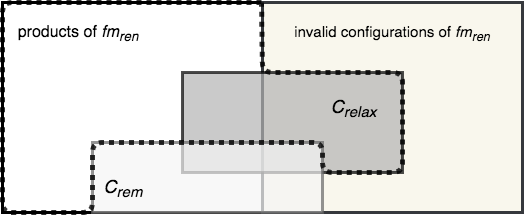
\includegraphics[width=.8\textwidth]{images/CremCrelax}
\end{center}
\caption{Added and removed products}
\label{fig:cremcrelax}
\end{figure}
%
\bb The new product set (in dotted line) is enriched by configurations identified by \CFrelax but deprived of the products identified by \CFrem; note that \CFrem could also remove some products added by \CFrelax.

If the user wants to include/exclude a specific configuration $c$, then (s)he simply adds $\fmToBool(c)$ to \CFrelax/\CFrem.\footnote{This is what we actually do in the experiments in Sect.~\ref{sec:experiments} where update requests are computed as differences between different versions of feature models, and \CFrelax and \CFrem can only be identified in terms of sets of configurations.}\be

\subsubsection{Well-formedness of an update request}\label{sec:wfUpdReq}

\bb We impose some constraints on the update request to be sure that the different change requirements are not contradictory and useful (i.e., they actually affect the product set):
%
\begin{compactenum}
\item \label{item:notCicleParentAndNotRemPar} Each added feature in \Fadd must have an ancestor in $\renamedFeatures\setminus\Frem$. This implies that it is not possible to remove by \Frem the parents $p$ of features added in \Fadd, i.e., $\Frem \cap (\bigcup_{f \in \Fadd} \{\parent{f}\}) = \emptyset$.
\item \label{item:notRemRen} It is not possible to remove features that have been renamed, i.e., $\Frem \cap (\bigcup_{f_i \in \Ftbr} \{\rename(f_i)\}) = \emptyset$.
\item \label{item:relaxNotRemFeat} Predicates in \CFrelax cannot predicate over features that have been removed in \Frem.
\item \label{item:relaxEffective} \CFrelax actually increases the set of products: for each $\rho_i$ in \CFrelax, there exists at least one non-valid configuration that satisfies $\rho_i$.
\item \label{item:remEffective} \CFrem actually deletes some products: for each $\gamma_i$ in \CFrem, there exists at least one product that satisfies $\gamma_i$.
\item \label{item:remNotBossy} \CFrem does not remove all the configurations that must be added by \CFrelax, i.e., for each $\rho_i$ and $\gamma_j$ there exists a configuration that satisfies $\rho_i$ (it must be added) and it does not satisfy $\gamma_j$.
\item \label{item:notIncons} The update request should be achievable by a consistent feature model (i.e., accepting at least one product) without dead features (i.e., each feature is selected in at least one model).
\end{compactenum}

Constraints
%\ref{item:notCicleParent}, \ref{item:notRemPar},
\ref{item:notCicleParentAndNotRemPar},
\ref{item:notRemRen}, and \ref{item:relaxNotRemFeat} can be easily checked directly at the syntactical level on the update request. If one of these constraints is not satisfied, the update request cannot be applied and we ask the user to fix it.

Checking constraints \ref{item:relaxEffective}, \ref{item:remEffective}, and \ref{item:remNotBossy}, instead, requires to reason over the propositional representation of \fmrenamed (i.e., $\fmToBool(\fmrenamed)$) and the predicates in \CFrelax and \CFrem; for example, checking constraint \ref{item:relaxEffective} consists in verifying that, for each $\rho_i \in \CFrelax$, $\neg \fmToBool(\fmrenamed) \wedge \rho_i$ is satisfiable. If one of these constraints is not satisfied, the update request is still consistent, although the corresponding change requirement is useless; in case of constraint violation, we warn the user about the useless change requirement and, if (s)he confirms that the change requirement is indeed not necessary, we continue the updating process without that requirement.

Checking constraint \ref{item:notIncons}, instead, requires to reason about the interaction of the different change requirements and can only be done after we define the target, as explained in the next section.

\begin{exmp}\label{ex:updReq}
Given the CAR SPL model shown in Fig.~\ref{fig:fmExample} and described in Ex.~\ref{ex:initialFM}, an update request could be the following\footnote{Note that the change requirement \Fadd is the same reported in~\cite{Pleuss2012} for the evolution from the third version (shown in Fig.~\ref{fig:fmExample}) to the fourth version of the CAR SPL; \CFrem, instead, is taken from the evolution from the first to the second version of the same SPL. In order to have a complete example, the other three change requirements have been identified by us; \Ftbr and \Frem resemble similar change requirements observed in literature, respectively in the SmartHome SPL~\cite{smartHomePaper} and in the CAR SPL~\cite{Pleuss2012}.}:
%
\begin{compactitem}
\item \textbf{Rename features} \Ftbr = \{\MonochromeRadioDisplay{}\} and \rename(\MonochromeRadioDisplay) = \RadioDisplay.
\item \textbf{Add features} \Fadd = \{\DVDEntertainment{}\} and \parent{\DVDEntertainment} = \MultimediaDevices.
\item \textbf{Remove features} \Frem = \{\OtherFeatures{}\}.
\item \textbf{Add products} \CFrelax = \{\MultimediaDevices $\wedge$ \Navigation $\wedge$ (\MonochromeNavigationDisplay $\leftrightarrow$ \ColorNavigationDisplay{})\}. We also want to allow products with support for navigation, and having both displays or having no display at all. 
\item \textbf{Remove products} \CFrem = \{$\Navigation \wedge \neg \Radio$\}. We want to exclude that navigation is present when the radio is not.
\end{compactitem}
\end{exmp}
\be

\subsubsection{Update request semantics}\label{sec:target}

\bb We here precisely define the semantics of an update request \UR. In order to do this, we define a formula that accepts and rejects configurations as the updated feature model should do.

In order to define the semantics of \Frem and \CFrelax, we need to be able to represent the feature model without some features. We exploit the approach used in~\cite{thum_abstract_2011} to remove features from feature models. To eliminate a feature $f$ from a propositional formula, we substitute $f$ by its possible values (true or false). \be

\begin{mydef}[Features removal]\label{def:featuresRem}
\bb Given a feature model \fm and a set of features $K = \{f_1,$ $\ldots,$ $f_k\}$ to remove, we recursively define $\filter(\fm, K)$ as follows:\be
%
\begin{equation*}
\filter(\fm, K) =\begin{cases}
\fmToBool(\fm) & {\rm if} \; K = \emptyset\\
\filter(\fm, K^\prime)[f \leftarrow \top] \vee \filter(\fm, K^\prime)[f \leftarrow \bot] & {\rm if} \; K = K^\prime \cup \{f\}\\
\end{cases}
\end{equation*}
%
\end{mydef}

\bb The formula $\filter(\fm, K)$ has as logical models the same models as $\fmToBool(\fm)$ except that all the features in $K$ have been removed.

Exploiting Def.~\ref{def:featuresRem}, the semantics of \Frem is captured by the formula
%
\[\phi_{\mathit{rem}} = \filter(\fmrenamed, \Frem)\] 
%
whose logical models (i.e., products) are those of \fmrenamed without the removed features.

In order to capture the semantics of a $\rho_i \in \CFrelax$, we need to characterize the set of configurations to add. These are those that satisfy $\rho_i$ but still respect the constraints of $\phi_{\mathit{rem}}$, except for those involving the features of $\rho_i$. This is captured by
%
\[\phi^i_{\mathit{relax}} = \filter(\phi_{\mathit{rem}}, \mathit{features}(\rho_i)) \wedge \rho_i\]
%
being $\mathit{features}$ a function returning the features (i.e., propositional variables) contained in a formula. The {\it filter} on $\phi_{\mathit{rem}}$ has the effect of making the features in $\rho_i$ unconstrained, i.e., it keeps only the constraints of $\phi_{\mathit{rem}}$ that do not {\it interfere} with $\rho_i$.

We can now build the formula that defines the semantics of the whole update request. We name the formula as {\it target} as it will be used as oracle to guide the proposed updating process (see Sect.~\ref{sec:process}).\be

\begin{mydef}[\textbf{Target}]\label{def:target}
\bb The target $t$ is a propositional formula whose models exactly correspond to the products of the desired updated feature model. Assume an update request $\UR = \{\rename, \parentna, \Frem, \CFrelax, \CFrem{}\}$ defined over a feature model \fm, with the functions \rename defined over \Ftbr and \parentna defined over \Fadd. Let \fmrenamed be the feature model renamed according to \rename; the target is defined as:\be
%
\begin{align*} 
t = & (\overbrace{\;\phi_{\mathit{rem}}\;}^{\parbox{18mm}{\footnotesize remove \Frem\\from products}} \vee \overbrace{\bigvee_{\rho_i \in \CFrelax} \phi^i_{\mathit{relax}}}^{\parbox{17mm}{\footnotesize add products}}) & \wedge
& \overbrace{\bigwedge_{f \in \Fadd} f \rightarrow \parent{f}}^{\parbox{24mm}{\footnotesize add \Fadd features only when possible}} \wedge \overbrace{\bigwedge_{f \in \Frem} \neg f}^{\parbox{17mm}{\footnotesize disable \Frem\\ features}} \wedge \overbrace{\bigwedge_{\gamma \in \CFrem} \neg \gamma}^{\parbox{12mm}{\footnotesize remove products}}
\end{align*}
\end{mydef}

\bb The target correctly rejects all the configurations of \CFrem and those containing a removed feature in \Frem; the accepted configurations are those in \CFrelax, plus those of $\phi_{\mathit{rem}}$ (i.e., the original feature model without the removed features) possibly extended with each added feature $f$ of \Fadd only when \parent{f} is present.

Note that the target correctly predicates over all the features $F_U = F^\prime \cup \Frem$: those of the original feature model (after renaming), those added, and those removed.\be

\paragraph{Checking the target}

\bb On the target, we can finally check constraint \ref{item:notIncons} described in Sect.~\ref{sec:wfUpdReq}, requiring that the update request does not produce anomalies.

First of all, we check that the target accepts at least one product (i.e., it is satisfiable); if not, we warn the user that the update request cannot be applied.

Moreover, we also check that each feature $f \in F^\prime$ can be actually selected in at least one product; it this is not possible, it means that $f$ is required to be dead in the final model. If this is the case, we warn the user about this and, if this is the intended behavior, we move $f$ in \Frem, so that we can directly try to remove it during the repairing process.\be

\subsection{Evolutionary updating process}\label{sec:process}

\bb Modifying the initial feature model \initFm such that it satisfies the update request as specified by the target is a challenging task. Note that, in general, there could be no \fmp that exactly adds and removes the specified configurations and features, unless {\it complex} cross-tree constraints are used. However, we claim that the usage of these constraints should be discouraged. Urli et al.~\cite{visualSupport} observe that ``they make FMs complex to understand and maintain'', Reinhartz-Berger et al.~\cite{ComprehendingFeatureModels} experimentally assessed that they are more difficult to understand than parent-child relationships (at least, by modelers who are unfamiliar with feature modeling), and Berger et al.~\cite{Berger2013} report that ``they are known to critically influence reasoners''. Also the authors of FeatureIDE noted that cross-tree constraints ``are harder to comprehend than simple tree constraints" and that ``relations among features should be rather expressed using the tree structure if possible''~\cite{FeatureIDEbook}. In this paper, we therefore avoid the addition of complex cross-tree constraints, as we not only aim at correctness (i.e., full achievement of the update request), but also at readability of the final model.
Some approaches that aim at simplifying complex constraints exist~\cite{knuppel_is_2017,vonRhein2015}, but they may diminish readability and other qualities, such as compactness, traceability, and maintainability.\footnote{In Sect.~\ref{sec:conclusions1}, we discuss how complex cross-tree constraints could be used to achieve all the change requirements and the issues that could be related to that approach.}

This paper proposes a heuristic approach that tries to achieve the update request {\it as much as possible}. In order to do this, we use the target as {\it oracle} to compute the {\it fault ratio}. The fault ratio tells how close we are to the correct solution. In Sect.~\ref{sec:correctness}, we give the definition of fault ratio and then, in Sect.~\ref{sec:updatingProcess}, we describe the updating process we propose.\be

\subsubsection{Correctness}\label{sec:correctness}

We can use the target to evaluate whether a feature model \fmp captures the desired change requirements, i.e., \fmp is equivalent to the target ($\models t \leftrightarrow \fmToBool(\fmp, F_U)$). In the following, we will only compare feature models \fmp whose features $F_{\fmp}$ are, at most, those in $F_U$, i.e., $F_{\fmp} \subseteq F_U$.

Although a feature model could not fulfill all the change requirements, it could satisfy them partially. We give a measure of the \emph{difference} between a feature model \fm (either the initial one \initFm or a modified one \fmp) and the target as follows.

\begin{mydef}[\textbf{Fault ratio}]\label{def:faultratio}
Given a feature model \fm and a target $t$, the \emph{fault ratio} of \fm w.r.t. $t$ is defined as follows:
%
\begin{equation*}
\FR(\fm, t) = \frac{|\mathit{AllConfs}(\fmToBool(\fm, F_U) \neq t, F_U)|}{2^{|F_U|}}
\end{equation*}
%
 where $\mathit{AllConfs}(\varphi, V)$ returns all the logical models of formula $\varphi$, i.e., all the truth assignments $m$ to propositional variables $V$, such that $m \models \varphi$.\footnote{In our approach, we represent formulas as Binary Decision Diagrams (BDDs) in JavaBDD that implements $|\mathit{AllConfs}|$ by means of the method $\mathtt{satCount}$ that directly computes the cardinality of the set without enumerating all the models.}
\end{mydef}

If the fault ratio is equal to 0, it means that \fm accepts as products the same configurations that are logical models of $t$; otherwise, there are some configurations that are wrongly evaluated by \fm, as shown in Fig.~\ref{fig:faults}: \fm could wrongly accept some configurations and/or wrongly refuse some others.

%
\begin{figure}[h]
\def\languageAll{(-1.2,-1.2) rectangle (2.2cm,1.2cm)}
\def\firstcircle{(0,0) circle (1cm)}
\def\circleS{(0:1cm) circle (1cm)}
\colorlet{circle edge}{black}
\tikzset{
filled1/.style={draw=circle edge},
filled2/.style={pattern=north east lines, pattern color=gray},
outline/.style={draw=circle edge, thick}}
\centering
\begin{tikzpicture}
\begin{scope}
\draw[filled2, even odd rule] \firstcircle \circleS;
\end{scope}
\begin{scope}
\end{scope}
\draw[outline] \firstcircle node [left=0mm] {\fm};
\draw[outline] \circleS node [right=2mm] {$t$};
\draw[outline] \languageAll node [right=0mm] {$2^{\mid F_U\mid}$};
\begin{customlegend}[legend cell align=left, %<= to align cells
legend entries={ % <= in the following there are the entries
{correct configurations}, 
{wrong configurations}
},
legend style={at={(6.5, 0.5)},font=\footnotesize}] % <= to define position and font legend
% the following are the "images" and numbers in the legend
\addlegendimage{area legend,filled1}
\addlegendimage{area legend,filled2}
\end{customlegend}
\end{tikzpicture}
\caption{Faults}
\label{fig:faults}
\end{figure}

\begin{exmp}
\bb Fig.~\ref{fig:exampleUpdatedFM} shows a possible updated model that exactly satisfies all the change requirements reported in Ex.~\ref{ex:updReq} for the model in Fig.~\ref{fig:fmExample}.\be 
%
\begin{figure}[htb!]
\centering
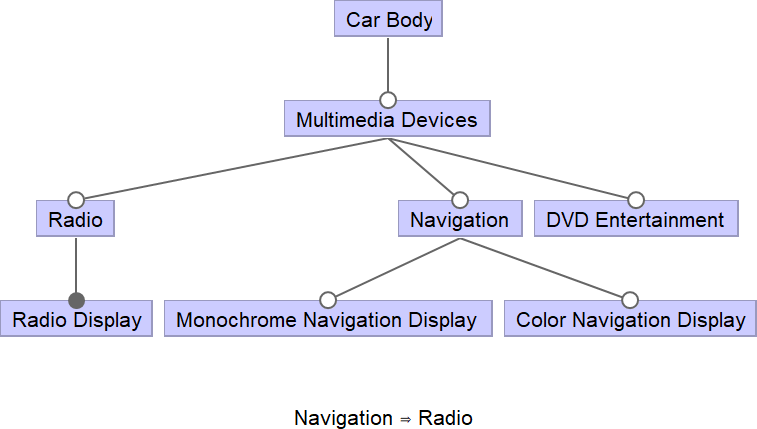
\includegraphics[height=5cm]{car2011_4paper}
\caption{Updated feature model}
\label{fig:exampleUpdatedFM}
\end{figure}
%
\bb Note that the fault ratio of the initial renamed feature model \initFm w.r.t. to the target $t$ (that corresponds to the final feature model) is $\frac{20}{2^9}$, as \initFm wrongly accepts all its 7 products and wrongly rejects all the 13 products of the target.\be
\end{exmp}

\subsubsection{Updating process}\label{sec:updatingProcess}

\bb
The process we propose to update an initial feature model \initFm, given an update request \UR, is depicted in Fig.~\ref{fig:approach}.
\be

%
\begin{figure*}[h]
\centering
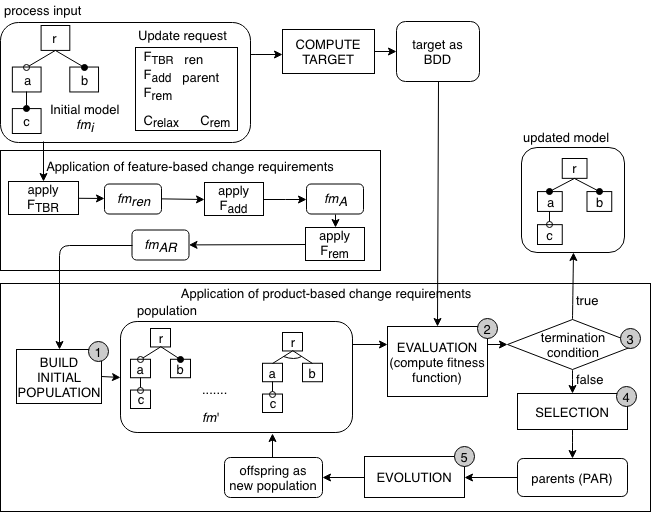
\includegraphics[width=\textwidth]{evolutionaryApproach}
\caption{Proposed evolutionary approach}
\label{fig:approach}
\end{figure*}
%

\bb
As initial step, we generate the target $t$ as a Binary Decision Diagram (BDD), as described in Def.~\ref{def:target}. Then, we start the updating process, that is composed of two consecutive macro-phases. We first try to deal with the feature-based change requirements (see Sect.~\ref{sec:featBasedChangeReqs}) and then with the product-based ones (see Sect.~\ref{sec:prodBasedChangeReqs}).
\be

\subsubsection{Dealing with feature-based change requirements}\label{sec:featBasedChangeReqs}

\bb 
First of all, we apply \Ftbr to rename features, obtaining the feature model \fmrenamed.

Then, we modify \fmrenamed in order to try to achieve the change requirements of \Fadd and \Frem. For each $f \in \Fadd$, we add $f$ as child of \parent{f} as follows: if \parent{f} is the father of an {\it Or} or an {\it Alternative} group, $f$ is added to the group; in all the other cases, it is added as {\it Optional} child of \parent{f}. We name as $\fm_{A}$ the feature model obtained after this step. Then, for each feature $f \in \Frem$, $f$ is removed from $\fm_{A}$ and replaced by its children $\mathit{Ch_f}$ (if any). The relation of the moved children $\mathit{Ch_f}$ of $f$ with their new parent $p$ is set according to the way FeatureIDE removes features~\cite{FeatureIDEbook}:
%
\begin{compactenum}
\item If $f$ was the only child of $p$, $p$ takes the group type of $f$. 
\item If $p$ has group type {\it And}, 
\begin{inparaenum}
\item if the children $\mathit{Ch_f}$ are in {\it And} relationship, they keep their type (either {\it Mandatory} or {\it Optional})
\item otherwise (they are in {\it Alternative} or {\it Or}), they are set to {\it Optional}.
\end{inparaenum}
\item Otherwise, if $p$ has group type {\it Alternative} or {\it Or}, features in $\mathit{Ch_f}$ are simply added to the group (regardless of their type).
\end{compactenum}


We name as $\fm_{\mathit{AR}}$ the feature model obtained after this step.

Note that the model $\fm_{\mathit{AR}}$ could still be not equivalent to the target, i.e., $\not \models t = \fmToBool(\fm_{\mathit{AR}}, F_U)$. This could be due to two reasons. First of all, the update request could also require to add as products configurations described by constraints in \CFrelax and/or remove configurations described by constraints in \CFrem. Moreover, the two previous transformations do not guarantee to precisely implement the required change requirements \Fadd and \Frem, and they could introduce some wrong configurations (either wrongly accepted or rejected). For example, in order to implement the addition of a feature $f$ with $\parent{f} = p$ and $p$ father of an alternative group, we add $f$ to the group; however, this is not the exact semantics of \Fadd that requires to duplicate the products containing $p$ and adding $f$ to them.
\be

\subsubsection{Dealing with product-based change requirements}\label{sec:prodBasedChangeReqs}
\bb
Starting from $\fm_{\mathit{AR}}$, we apply an evolutionary updating approach to try to obtain an updated feature model equivalent to the target. The process is an instance of classical evolutionary algorithms~\cite{Eiben2003}; an evolutionary algorithm can be understood (in a metaphor-free language~\cite{metaheuristicsMetaphor}) as an optimization problem in which different solutions are modified by random changes and their quality is checked by an objective function. Precisely, the steps are as follows:
%
\begin{compactenum}
\item \textbf{Initial population}: at the beginning, a population $P$ is created. $P$ is a set of candidate solutions.
\item \textbf{Iteration}: the following steps are repeatedly executed:
\begin{compactenum}
\item \textbf{Evaluation}: each member of the population $P$ is evaluated using a given \emph{fitness function}, representing the objective function.
\item \textbf{Termination}: a termination condition is checked in order to decide whether to start the next iteration. If the termination condition holds, the candidate with the best \emph{fitness value} is returned as final model.
\item \textbf{Selection} (\emph{Survival of the Fittest}): some members of $P$ having the best values of the fitness function are selected as parents of the next generation and collected in the set \PAR.
\item \textbf{Evolution}: parents \PAR are mutated to obtain the \emph{offspring} to be used as population in the next iteration. The mutation performs random changes suitable to improve the existing solutions.
\end{compactenum}
\end{compactenum}

In our approach, we assume that the population $P$ is a multiset (i.e., possibly containing duplicated elements) with fixed size $M$ equal to $H \cdot |F^\prime|$, where $H$ is a parameter of the process. In the following, we describe each step in details.
\be

\paragraph{\bf Initial population}%\label{sec:initPopulation}

\bb
As initial population, we generate the set $P$ by cloning $\fm_{\mathit{AR}}$ $M$ times (step 1 in Fig.~\ref{fig:approach}). In this way, if $\fm_{\mathit{AR}}$ is already correct, it will be returned as final model in the \emph{termination condition} phase.
\be

\paragraph{\bf Evaluation}%\label{sec:evaluation1}
\bb As first step of each iteration (step 2 in Fig.~\ref{fig:approach}), each candidate member \fmp of the population $P$ is evaluated using a \emph{fitness function} that tells how \emph{good} the member is in achieving the overall goal. We define the fitness function both in terms of fault ratio (see Def.~\ref{def:faultratio}) and of {\it complexity} of the model structure. Indeed, we would like to avoid that, during the updating process, the feature model becomes unreadable, unnecessarily complex, and difficult to maintain~\cite{Berger2013,visualSupport,ComprehendingFeatureModels,FeatureIDEbook}. We have decided to consider, at least initially, the number of cross-tree constraints as indicator of complexity, since the constraints among features should be expressed by structural relationships and cross-tree constraints should be used only when really necessary. We introduce the following fitness function:\be
%
\begin{equation}\label{eq:fitness}
\fitness(\fmp) = 1 - \FR(\fmp, t) - k \times \mathit{ctc}(\fmp)
\end{equation}
%
\bb where $\mathit{ctc}$ is a function returning the number of cross-tree constraints of a feature model and $k$ a constant. In our approach, the quality of a candidate must be mainly given by the percentage of configurations that it evaluates correctly, i.e., $1 - \FR(\fmp, t)$; if a candidate $c_1$ evaluates correctly more configurations than a candidate $c_2$, its fitness should be guaranteed to be greater than that of $c_2$. However, for models having the same fault ratio, the fitness should penalize those that are structurally more complex. In order to obtain this effect, we use as $k$:\be
%
\begin{equation}\label{eq:kFitness}
k = \frac{1}{{2^{|F_U|} \times 2|F_U|^2}}
\end{equation}

\bb Note that $2 |F_U|^2$ is a safe strict upper bound on the number of cross-tree constraints among the features of the feature model. Indeed, among the possible $2|F_U|^2$ cross-tree constraints, some of them are not introduced because redundant (e.g., two {\it excludes} constraints between $(a,b)$ and $(b,a)$ are redundant and only one is necessary). Therefore, the term $\frac{\mathit{ctc}(\fmp)}{2^{|F_U|} \times 2|F_U|^2}$ is guaranteed to be less than $\frac{1}{2^{|F_U|}}$ that is the minimal possible variation of the fault ratio due to the change of evaluation of a single configuration. This means that the term can only affect the ranking of feature models having the same fault ratio.\be

\paragraph{\bf Termination condition}%\label{sec:termination}
\bb In this step (step 3 in Fig.~\ref{fig:approach}), the process checks whether at least one of the following conditions is met:
%
\begin{compactitem}
\item a defined level of fitness \thF is reached, i.e., there exists an \fmp in $P$ with $\fitness(\fmp) \ge \thF$. For example, $\thF=1$ means that we want to obtain a completely correct model without any cross-tree constraint; with $\thF = 1 - \frac{1}{2^{|F_U|} + 1}$, instead, we still want to have a correct model, but we allow to have any number of cross-tree constraints;
\item in the previous \thNI iterations there has been no improvement of the fitness value of the best candidate;
\item a maximum number \thI of iterations have been executed;
\item a total time threshold \thT has been reached.
\end{compactitem}

If at least one of the previous conditions holds, the \fmp in $P$ with the highest fitness value is returned as final model.\footnote{If there is more than one model with the highest fitness value, we randomly select one of these models.}\be

\paragraph{\bf Selection}%\label{sec:selection}
\bb In the \emph{selection} step (step 4 in Fig.~\ref{fig:approach}), starting from population $P$, a multiset of \emph{parents} \PAR of size $p$ is built, being $p$ a parameter of the evolutionary process. Different selection strategies have been proposed in literature:
%
\begin{compactitem}
\item \emph{Truncation}: it selects the first $n = \left\lceil K\cdot|P| \right\rceil$ members of the population with the highest fitness value, where $K$ is a parameter specifying a percentage of the population ($0 < K \le 1$). Then, the first $n$ elements are added to \PAR as many times as necessary to reach the size $p$. Such strategy could result in premature convergence, as candidates with lower fitness values are not given the opportunity to improve their fitness.
\item \emph{Roulette wheel}: $p$ members of the population are selected randomly; each member can be selected with a probability proportional to its fitness value. Note that one or more individuals could be selected multiple times.
\item \emph{Rank}: it is similar to roulette wheel, except that the selection probability is proportional to the relative fitness rather than the absolute fitness, i.e., the probability of selecting a member is inversely proportional to its ranking number (where the member with highest fitness has ranking number 1). This strategy tends to avoid premature convergence by mitigating the selection pressure that comes from large differences in fitness values (as it happens in truncation selection).
\end{compactitem}\be

\paragraph{\bf Evolution}%\label{sec:evolution}
\bb In the \emph{evolution} step (step 5 in Fig.~\ref{fig:approach}), the parents \PAR are used to generate the \emph{offspring} that constitutes the population of the next generation.

The idea we assume here is that the feature model should be updated applying a limited number of mutations. Making updates through the use of mutation operators has the benefit of reducing the risk of loss of domain knowledge, by changing the feature model as less as possible. Note that this assumption is similar to the competent programmer hypothesis~\cite{surveyMutationTesting} that assumes that the user has defined the artifact close to the correct one. If our approach is used for removing faults, we can directly rely on the competent programmer hypothesis. On the other hand, if the approach is used to evolve the feature model to align it with the SPL, we can still assume that the mutation operators are sufficient to obtain the updated model; indeed, it is unlikely that the updated version of the feature model should be too different from the initial one.

In order to build the next population $P$, we mutate all the feature models in \PAR using the operators presented in Table~\ref{tab:mutOperators}.\be

%
\begin{table}[!htb]
\caption{Mutation operators}
\resizebox{\textwidth}{!}{%
\centering
\begin{tabular}{rl}
\toprule
Name & Description\\
\midrule
\OptToMan & an {\it optional} feature is changed to {\it mandatory}\\
\ManToOpt & a {\it mandatory} feature is changed to {\it optional}\\
\OrToAl & an {\it or} group is changed to {\it alternative}\\
\OrToAnd & an {\it or} group is changed to {\it and} with all children {\it mandatory}\\
\OrToAndOpt & an {\it or} group is changed to {\it and} with all children {\it optional}\\
\AlToOr & an {\it alternative} group is changed to {\it or}\\
\AlToAnd & an {\it alternative} group is changed to {\it and} with all children {\it mandatory}\\
\AlToAndOpt & an {\it alternative} group is changed to {\it and} with all children {\it optional}\\
\AndToAl & an {\it and} group is changed to {\it alternative}\\
\AndToOr & an {\it and} group is changed to {\it or}\\
\midrule
\PullUp & a feature is moved as sibling of its parent\\
\PushDown & a feature is moved as child of one of its siblings\\
\PullUpChildren & all children of a feature are moved as siblings of their parent\\
\PushDownSiblings & all siblings of a feature are moved as children of that feature\\
\midrule
\DelConstr & a cross-tree constraint ({\it requires} or {\it excludes}) is deleted\\
\ReqToExcl & a {\it requires} constraint is changed to an {\it excludes} constraint\\
\ExclToReq & an {\it excludes} constraint is changed to a {\it requires} constraint\\
\Creq & a {\it requires} constraint is created\\
\Cexc & an {\it excludes} constraint is created\\
\bottomrule
\end{tabular}}
\label{tab:mutOperators}
\end{table}
%

\bb We set an upper bound $M$ to the size of the new population. If the mutation operators generate a maximum of $M$ mutants, we take all of them as the new population, otherwise we randomly select $M$ of them. In our approach, the offspring replaces the entire population.

{\it Description of mutation operators}
In~\cite{icst2015}, we have proposed some mutation operators for feature models, divided in \textit{feature-based} and \textit{constraint-based} operators that are a subset of the edit operations identified in~\cite{Burdek2016}. We use eight of the feature-based mutation operators proposed in~\cite{icst2015}, and introduce two new ones (\OrToAndOpt and \AlToAndOpt) that provide slightly different versions of \OrToAnd and \AlToAnd. Moreover, we also introduce two operators that permit to move a feature as sibling of the parent (\PullUp) or as child of one its siblings (\PushDown); we also introduce two versions of these operators that move all the children of a feature (\PullUpChildren) and all the siblings of a feature (\PushDownSiblings). Note that we do not allow the movement of a feature in any part of the feature model as this would produce too many mutants and could change too much the structure of the feature model. However, if in order to obtain the correct feature model a feature should be moved {\it far} from its current position, this is still obtainable by a suitable sequence of \PullUp and \PushDown mutations.

Finally, we use all the \textit{constraint-based} operators\footnote{Note that the mutation operator \DelConstr corresponds to operator \MC described in~\cite{icst2015}.} proposed in~\cite{icst2015}, and introduce two new ones (\Creq, \Cexc) to create {\it requires} and {\it excludes} constraints; in order to limit the number of generated mutants, we only create constraints among features that belong to different sub-trees of the feature model, i.e., neither feature of the constraint is ancestor of the other. Moreover, we avoid to create constraints that would be redundant or that would introduce dead features: for instance, $A \rightarrow \neg B$ is not added if $A \rightarrow B$ is already present in the model, because A would become a dead feature.

Although we allow feature models with constraints also in general form, we decided to not modify them, nor introduce new ones, in order to avoid the introduction of too many mutants and to achieve better readability of the final model.

In general, we cannot evaluate a priori if a mutant introduces an anomaly; therefore, for each mutant, we check if it is infeasible, it contains redundant constraints, or it has dead features. If it has any of these anomalies, we do not select it.\be

\subsection{Experiments}\label{sec:experiments}

\bb The process\footnote{The code is available at \url{https://github.com/fmselab/eafmupdate}} has been implemented in Java by using Watchmaker\footnote{\url{https://watchmaker.uncommons.org/}} as evolutionary framework, FeatureIDE~\cite{FeatureIDEbook} to represent and mutate feature models, and JavaBDD for BDDs manipulation. 

We conducted a set of experiments to evaluate the proposed evolutionary approach; they have been executed on a Windows 10 system with an Intel i7-3770 3.40GHz processor, and 16 GB RAM.\be

\subsubsection{Benchmarks}\label{sec:benchmarks1}

\bb For the experiments, we used two sets of benchmarks, both shown in Table~\ref{tab:benchmarks}.\be
%
\begin{table}[!htb]
\caption{Benchmark properties}
\centering
\resizebox{\columnwidth}{!}{%
\begin{tabular}{clcc|ccccc} 
\toprule
& & \multicolumn{2}{c|}{model size} & \multicolumn{5}{c}{\UR size}\\
& SPL & input & target & $\vert \Ftbr \vert$ & $\vert \Fadd \vert$ & $\vert \Frem \vert$ & $\vert \CFrelax \vert$ & $\vert \CFrem \vert$\\
\midrule
\multirow{12}*{\rotatebox{90}{\small \benchReal}}
&{\tt MobileMedia d1} (V5..8) & 18.7 (15-23) & 22.3 (18-26) & 11.3 (1-17) & 4 (3-5) & 0.33 (0-1) & 26.7 (0-48) & 258 (24-560) \\
&{\tt MobileMedia d2} (V5..8) & 16.5 (15-18) & 24.5 (23-26) & 12 (11-13) & 8 (8-8) & 0 (0-0) & 64 (48-80) & 536 (528-544) \\
&{\tt MobileMedia d3} (V5,V8) &15 & 26 & 9 & 11 & 0 & 80 & 1648 \\
&{\tt HelpSystem} (V1, V2) & 25 & 26 & 0 & 1 & 0 & 672 & 2016 \\
&{\tt SmartHome} (V2.0, V2.2) & 39 & 60 & 12 & 23 & 2 & $1.92 \times 10^{9}$ & $2.31 \times 10^{10}$ \\
&{\tt ERP\_SPL} (V1, V2) & 43 & 58 & 0 & 15 & 0 & 0 & $1.51 \times 10^{7}$ \\
&{\tt PPU d1} (V1..9) & 13.9 (9-17) & 14.9 (11-17) & 0 (0-0) & 1.13 (0-4) & 0.125 (0-1) & 3.75 (0-27) & 27.8 (0-183) \\
&{\tt PPU d2} (V1..9) & 13.4 (9-17) & 15.4 (11-17) & 0 (0-0) & 2.14 (0-6) & 0.142 (0-1) & 9 (0-27) & 54.4 (0-243) \\
&{\tt PPU d3} (V1..9) & 12.8 (9-17) & 16.2 (13-17) & 0 (0-0) & 3.5 (1-6) & 0.167 (0-1) & 16 (0-27) & 77.5 (9-156) \\
&{\tt CAR d1} (V2009..2012) & 7 (6-8) & 9.33 (7-13) & 0 (0-0) & 2.67 (1-5) & 0.333 (0-1) & 5 (0-13) & 16 (1-40) \\
&{\tt CAR d2} (V2009..2012) & 6.5 (6-7) & 10.5 (8-13) & 0 (0-0) & 4.5 (3-6) & 0.5 (0-1) & 6 (0-12) & 34 (9-59) \\
&{\tt CAR d3} (V2009,V2012) & 6 & 13 & 0 & 7 & 0 & 0 & 87 \\
\midrule
\multirow{4}*{\rotatebox{90}{\small \benchMut}}
%& {\tt Example} & 4 & 4 & 0 & 0 & 0 & 0.41 (0-2) & 0.68 (0-2)\\
& {\tt Register} & 11 & 11 & 0 & 0 & 0 & 11.85 (0-40) & 62.28 (0-210)\\
& {\tt Graph} & 6 & 6 & 0 & 0 & 0 & 12.71 (0-28) & 0 (0-0)\\
&{\tt Aircraft} & 13 & 13 & 0 & 0 & 0 & 196.86 (0-315) & 53.53 (0-365)\\
& {\tt Connector} & 20 & 20 & 0 & 0 & 0 & 8.23 (0-18) & 26.02 (0-336)\\
\bottomrule
\end{tabular}
}
\label{tab:benchmarks}
\end{table}

\paragraph{Real models}
\bb The first benchmark set \benchReal is constituted by SPLs described in literature for which different versions of their feature model have been developed. First, we have identified in the SPLOT repository\footnote{\url{http://52.32.1.180:8080/SPLOT/feature_model_repository.html}} four SPLs that evolved over time:
%
\begin{compactitem}
\item {\tt MobileMedia}: a program to manipulate multimedia on mobile devices (four versions)~\cite{multimediaPaper};
\item {\tt HelpSystem}: a cyber-physical system with multiple sensors (two versions)~\cite{helpSystemPaper};
\item {\tt SmartHome}: a set of smart house components (two versions)~\cite{smartHomePaper};
\item {\tt ERP\_SPL}: an Enterprise Resource Planner (two versions).
\end{compactitem}
%
Then, we have also considered the industrial case of a Pick-and-Place Unit ({\tt PPU})~\cite{Burdek2016}; for this system, the feature model has been changed eight times to adapt to new requirements (therefore, there are nine feature models available~\cite{Burdek2016}). Finally, we have also considered the product line model of a {\tt CAR}~\cite{Pleuss2012}, for which four different feature models have been produced.

For each SPL, we identified couples (\initFm, $\fm_t$) of their feature models: the latest version was considered as target model\footnote{Note that, in the real usage of our approach, we do not have a target feature model, but an update request \UR from which we generate the target as propositional formula.} $\fm_t$, and the oldest one as the initial model \initFm we want to update. For SPLs with more than two feature models, in addition to couples of feature models of consecutive versions, we also considered models with version distance 2 and 3 (in the table, d1, d2, and d3 indicate the distance). In this way, we attempt to reproduce update requests of different complexity. In total, \benchReal contains 36 couples of models.\be

\paragraph{Generated models}
\bb The second benchmark set \benchMut has been built with the aim of evaluating our approach under the assumption we did in Sect.~\ref{sec:prodBasedChangeReqs} that mutation operators are sufficient to update the feature model. We selected four feature models developed for four SPLs (for which only one model is available):
%
\begin{compactitem}
\item {\tt Register}: a register of supermarkets, adapted from~\cite{Shimbara2015};
\item {\tt Graph}: a graph library;
\item {\tt Aircraft}: the configurations of the wing, the engine, and the materials of airplane models;
\item {\tt Connector}: IP connection configurations.
\end{compactitem}
%
From these models (used as target models $\fm_t$), we automatically generated other versions to be used as input models \initFm; we randomly mutated the target models (using 1 to 10 mutations), applying the operators described in Table~\ref{tab:mutOperators}. For each target model, we generated 100 input models. Therefore, \benchMut contains 400 couples.\be

\subsubsection{Deriving the update request}

\bb In the devised usage of the approach, the user should specify the update request that must be provided as input to the evolutionary process; however, for our experiments, we do not have any update request available. Therefore, we automatically generated an update request \UR from the initial feature model \initFm and the target feature model $\fm_t$ of each couple (\initFm, $\fm_t$) of the benchmarks.

In order to detect renamed features in \Ftbr, we manually inspected the two feature models and produced the renamed model \fmrenamed. Then, from \fmrenamed and $\fm_t$, we automatically identified the differences of their features for building \Fadd and \Frem; moreover, using their BDD representation, we identified the configurations that are differently evaluated in order to build \CFrelax and \CFrem (we built a predicate for each wrongly evaluated configuration\footnote{Note that, in this way, the sets \CFrelax and \CFrem are very large because they contain a predicate for each added and removed configuration. However, in a real setting, the user should specify predicates capturing sets of configurations and so the sets should be much smaller.}). Note that configurations that are added and removed by \Fadd and \Frem are not also specified in \CFrelax and \CFrem.

Table~\ref{tab:benchmarks} reports, for all the benchmarks, the size of the input and target models in terms of number of features, and the number of requirements of the update request. For the SPLs in \benchReal having more than one couple of feature models, the reported values are aggregated by distance; for each SPL in \benchMut, the values are aggregated among its 100 input models. For these aggregated models, we report the average, minimum, and maximum number of elements in the update request. In \benchMut, since we did not add or remove features for producing the input models, their size is the same of that of the target model and so \Fadd and \Frem are empty; moreover, we do not even rename features and so also \Ftbr is empty.\be

\subsubsection{Analysis}\label{sec:analysis}

\bb We now evaluate the proposed approach by a series of research questions. In these experiments, we set the parameters of the termination conditions as follows: \thF to $1 - \frac{\mathit{ctc}(\initFm)}{{2^{|F_U|} \times 2|F_U|^2}}$, \thNI to 15, \thI to 25, and \thT to 30 minutes. Note that the value chosen for \thF requires to have a totally correct model, with at most the same number of cross-tree constraints of the starting feature model. The parameter $H$ used to determine the maximum population size $M$ (as defined in Sect.~\ref{sec:prodBasedChangeReqs}) has been set to 5, and the parameter $p$ of the selection phase has been set to $\nicefrac{M}{2}$. All the reported data are the averages of 30 runs.

In~\cite{arcaini_evolutionary_2018}, we experimented the effect of the different selection policies of the evolutionary approach and we found that truncation with $K$=5\% is the best policy in terms of fault ratio reduction, and the second best as execution time. Therefore, we here select it as selection policy and evaluate the approach using other research questions.

\researchquestion{Is the proposed approach able to achieve the change requirements specified by the update request?}

For each benchmark SPL, Table~\ref{tab:processPerformance} reports (among other things) the initial and final values of \FR, and the \FR reduction.\be

%
\begin{table}[H]
\caption{Performance of the updating process}
\resizebox{\textwidth}{!}{%
\centering
\setlength\tabcolsep{2pt} 
\begin{tabular}{c l rrrrrrrrr}
\toprule
& SPL & \shortstack{time\\(s)} & \shortstack{initial\\FR (\%)} & \shortstack{final\\FR (\%)} & \shortstack{FR\\reduction (\%)} & \shortstack{\# \\ iterations} & \shortstack{sem.\\eq. (\%)} & \shortstack{synt.\\eq. (\%)} & ctc & ED \\
\midrule
\multirow{12}*{\rotatebox{90}{\small \benchReal}} &   {\tt MobileMedia d1}  & 71.11 &  4.17e-03 & 1.10e-04 & 96.03 & 8.42 & 64.44 & 17.78 &   0.23 &   14.86 \\ 
&  {\tt MobileMedia d2} & 157.98 &  3.90e-03 & 4.41e-04 & 86.54 &     16.00 &      0.00 &      0.00 &   0.63 &   34.32 \\ 
&  {\tt MobileMedia d3} & 178.46 &  2.57e-03 & 3.57e-04 & 86.13 &     16.00 &      0.00 &      0.00 &       0.80 &   36.97 \\ 
&  {\tt HelpSystem} & 112.41 &  4.01e-03 & 1.24e-04 & 96.92 &    8.80 & 86.67 &      0.00 &    5.57 &   25.53 \\ 
&  {\tt SmartHome} & 1990.40 & 7.24e-07 & 8.39e-08 & 88.42 &    6.10 &      0.00 &      0.00 &   0.43 &     57.60 \\ 
& {\tt ERP\_SPL} & 2014.30 & 5.24e-09 & 8.86e-10 & 83.08 &      6.00 &      0.00 &      0.00 &   0.43 &     18.80 \\ 
& {\tt PPU d1} &  5.98 &    0.09 &  2.27e-03 & 97.44 & 3.88 & 86.67 & 48.33 &    1.23 &      7.40 \\ 
& {\tt PPU d2} & 10.23 &    0.10 &   0.54e-03 & 96.48 & 6.84 & 68.57 & 36.67 &    1.39 &   11.63 \\ 
& {\tt PPU d3} & 15.90 &   0.09 &   0.01 & 87.43 & 9.69 & 48.89 & 28.89 &    1.94 &   17.04 \\ 
& {\tt CAR d1} &  3.85 &     1.13 &   0.25 & 69.81 & 11.18 & 57.78 & 6.67 &   0.77 &   8.02 \\ 
& {\tt CAR d2} & 4.21 &     1.31 &    0.17 & 80.31 & 10.52 &     50.00 &      0.00 &    1.83 &    10.15 \\ 
& {\tt CAR d3}  & 6.59 &      1.06 &    0.37 & 65.52 &     16.00 &      0.00 &      0.00 &    2.37 &   20.13 \\ 
\midrule
\multirow{4}*{\rotatebox{90}{\small \benchMut}}
 & {\tt Register} &   4.35 &     3.62 &    0.17 & 95.84 &  7.15 & 80.27 &   65.20 &   0.22 &   2.32 \\ 
 & {\tt Graph} &  0.12 &     19.86 &          0.00 &    100.00 & 1.76 &    100.00 & 99.03 & 2.67e-03 & 0.02 \\ 
 & {\tt Aircraft} &  8.09 &     3.06 &   0.07 & 97.49 & 6.58 & 84.53 & 68.63 &   0.29 &   2.89 \\ 
 & {\tt Connector} & 28.68 &  3.27e-03 & 6.87e-05 & 98.11 & 5.80 &     94.00 & 68.47 &   0.20 &    2.27 \\ 
\bottomrule
\end{tabular}
}
\label{tab:processPerformance}
\end{table}
%

\bb For the models in \benchReal, the table reports the averages among couples at the same distance; for the models in \benchMut, instead, it reports the averages among the 100 input models of each SPL.\footnote{Non-aggregated results are reported online at \url{http://foselab.unibg.it/eafmupdate/}} We observe that for all models we can reduce the fault ratio of at least 65\%, with an average of 89.1\%. Comparing the two benchmark sets, we notice that the reduction is higher in \benchMut (on average, 97.86\%) than in \benchReal (on average, 86.15\%); this means that, as expected, if the assumption that the models can be updated using the proposed mutation operators holds, the approach behaves very well. However, also for general models as those in \benchReal, the performance of the approach is quite good.

\researchquestion{Which is the computational effort of the proposed approach?}
We are here interested in the effort required by the proposed approach in terms of computation time and iterations of the evolutionary process. Table~\ref{tab:processPerformance} also reports the total execution time of our process and the number of iterations of the evolutionary approach. For all but two models, the process takes at most 179 seconds; as expected, smaller models (as {\tt CAR}, {\tt Graph}, and {\tt Register}) are updated faster than larger models (as {\tt Mobile\-Media}, {\tt Help\-System}, {\tt Smart\-Home}, and {\tt ERP\_SPL}). We observe that the process terminates when one of these three terminating conditions occurs:
%
\begin{inparaenum}[(i)]
\item \thF, i.e., the model is completely updated (as in {\tt Help\-System} and {\tt Graph}),
\item \thT, i.e., the timeout has occurred (as in {\tt Smart\-Home} and {\tt ERP\_SPL}\footnote{Note that the time for these two models is around 3.5 minutes above the threshold \thT of 30 minutes; indeed, the terminating condition is checked at the end of an evolution step, but the threshold could be overcame during the step.}), or
\item \thNI, i.e., no fitness improvement has been observed in the previous 15 iterations (as, for example, all the models of {\tt Mobile\-Media d2} and {\tt d3}, and those of {\tt CAR d3}).
\end{inparaenum}
%
Note that the process never terminates because of the maximum number of iterations \thI.

\researchquestion{Is there a relation between the initial fault ratio and its \emph{updatability}?}

We are here interested in investigating whether there is a relation between the initial fault ratio and its reduction. Fig.~\ref{fig:frRepair} shows, for each benchmark model (a point in the plot), its initial fault ratio and the fault ratio reduction. \be

%
\begin{figure*}[h]
\centering
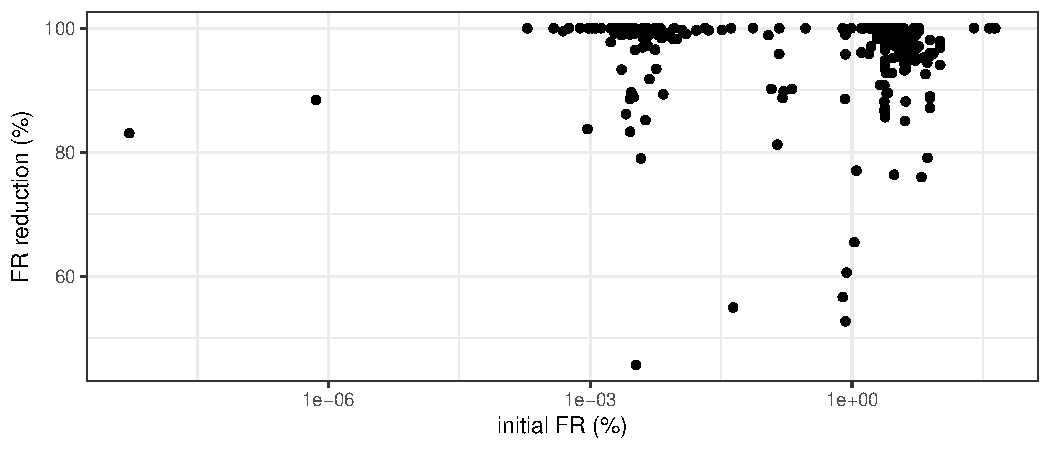
\includegraphics[width=.8\textwidth]{frRepairRed}
\caption{Relation between the initial fault ratio and the fault ratio reduction}
\label{fig:frRepair}
\end{figure*}
%

\bb It seems that there is no proper correlation: we reduce (or do not reduce) the fault ratio in the same proportion among models having different initial fault ratios. We checked the correlation with the Spearman rank-order correlation coefficient~\cite{Wohlin2012}, and indeed we found a value of 0.23 indicating almost no correlation~\cite{hinkle2003applied}.

\researchquestion{Are the final models similar to those produced by SPL designers?}

The main aim of the proposed approach is to obtain a feature model that satisfies all the change requirements; to this purpose, we use the fault ratio as measure of model correctness. However, the final model we obtain, although correct, may be not readable by and not useful for an SPL designer. Although we could not ask real SPL designers to validate our models in terms of usefulness and readability, we have access to models developed by SPL designers to achieve the same update requests we tackled in the experiments (models $\fm_t$ used as target in the experiments). We can assume that SPL designers are likely to find our models useful if models produced by our process are similar to their models. We therefore measure the {\it readability} of the final model of our process in terms of {\it distance} from the model $\fm_t$ developed by a designer for the same update request. We compute the {\it edit distance}~\cite{pawlik_efficient_2015,pawlik_tree_2016} of the final model $\fm_f$ from $\fm_t$, defined as the number of {\it edits} (insertion, deletion, and rename of tree nodes) that we have to apply to $\fm_f$ in order to obtain $\fm_t$.\footnote{Note that these edit operations are more fine-grained than our mutation operators and we are always able to compute the distance between two feature models.} Table~\ref{tab:processPerformance} reports also the edit distance (ED) to the target model (average among the models), and the percentage of models that are syntactically equal and semantically equivalent to the target model. Of course, models not completely updated are not syntactically equal to the target and have edit distance greater than 0. Completely correct models (semantically equivalent) are often also syntactically equal (for example, 86.67\% of the {\tt PPU d1} models are semantically equivalent and 48.33\% are also syntactically equal); however, there are some correct final models that are different from the target model $\fm_t$ (for example, {\tt HelpSystem} is completely updated 86.67\% of the times, but always in a different way than $\fm_t$).


\researchquestion{Does considering the number of cross-tree constraints in the fitness impact the final results?}

As explained in Sect.~\ref{sec:prodBasedChangeReqs}, our fitness function (see Eq.~\ref{eq:fitness}) can also take into consideration the number of cross-tree constraints ($\mathit{ctc}$); the value we selected for $k$ (see Eq.~\ref{eq:kFitness}) has the aim of penalizing models with higher $\mathit{ctc}$ at the same fault ratio (in order to limit the insertion of such constraints and instead give precedence to changes of the parental relations). In order to assess the impact of this choice, we have executed the same experiments presented before with $k=0$ in the fitness function (that becomes $\fitness(\fmp) = 1 - \FR(\fmp, t)$) and $\thT=1$. Table~\ref{tab:performanceVsConstraints} reports the data in terms of average fault ratio reduction, percentage of semantically equivalent, percentage of syntactically equal models, and the average number of cross-tree constraints.
\be

%
\begin{table}[H]
\caption{Performance of the updating process with the two versions of the fitness}
\resizebox{1\textwidth}{!}{%
\centering
\setlength\tabcolsep{2pt} 
\begin{tabular}{llrrrr|rrrr}
\toprule
& SPL & \multicolumn{4}{c}{Fitness without constr. ($k=0$)} & \multicolumn{4}{c}{Fitness with constr. ($k$ as in Eq.~\ref{eq:kFitness})}\\
\midrule
& & \shortstack{FR\\reduction (\%)} & \shortstack{sem.\\eq. (\%)} & \shortstack{synt.\\eq. (\%)} & ctc & \shortstack{FR\\reduction (\%)} & \shortstack{sem.\\eq. (\%)} & \shortstack{synt.\\eq. (\%)} & ctc \\
\midrule
\multirow{12}*{\rotatebox{90}{\small \benchReal}} & {\tt MobileMedia d1} & 94.10 &  61.11 & 17.78 & 0.69 &  96.03 &  64.44 & 17.78 & 0.23 \\
& {\tt MobileMedia d2} & 84.83 &   0.00 &  0.00 & 1.85 &  86.54 &   0.00 &  0.00 & 0.63 \\ 
& {\tt MobileMedia d3} & 85.16 &   0.00 &  0.00 & 2.43 &  86.13 &   0.00 &  0.00 & 0.80 \\ 
& {\tt HelpSystem} & 97.22 &  86.67 &  0.00 & 5.57 &  96.92 &  86.67 &  0.00 & 5.57 \\ 
& {\tt SmartHome} &   88.42 &   0.00 &  0.00 & 0.53 &  88.42 &   0.00 &  0.00 & 0.43 \\ 
& {\tt ERP\_SPL} &   82.96 &   0.00 &  0.00 & 0.40 &  83.08 &   0.00 &  0.00 & 0.43 \\ 
& {\tt PPU d1} & 98.10 &  87.50 & 45.83 & 1.62 &  97.44 &  86.67 & 48.33 & 1.23 \\ 
& {\tt PPU d2} & 95.89 &  68.57 & 37.14 & 2.11 &  96.48 &  68.57 & 36.67 & 1.39 \\ 
& {\tt PPU d3} & 87.25 &  50.00 & 27.22 & 2.95 &  87.43 &  48.89 & 28.89 & 1.94 \\ 
& {\tt CAR d1}  & 73.61 &  55.56 &  3.33 & 1.89 &  69.81 &  57.78 &  6.67 & 0.77 \\ 
& {\tt CAR d2}  & 78.06 &  45.00 &  0.00 & 3.22 &  80.31 &  50.00 &  0.00 & 1.83 \\ 
& {\tt CAR d3}  & 62.80 &   0.00 &  0.00 & 4.63 &  65.52 &   0.00 &  0.00 & 2.37 \\ 
\midrule
\multirow{4}*{\rotatebox{90}{\small \benchMut}} & {\tt Register} &   96.11 &  82.70 & 64.03 & 0.60 &  95.84 &  80.27 & 65.20 & 0.22 \\ 
& {\tt Graph} & 100.00 & 100.00 & 99.37 & 0.00 & 100.00 & 100.00 & 99.03 & 0.00 \\ 
& {\tt Aircraft} &  97.43 &  85.97 & 68.73 & 0.42 &  97.49 &  84.53 & 68.63 & 0.29 \\ 
& {\tt Connector} & 98.05 &  93.70 & 63.00 & 0.48 &  98.11 &  94.00 & 68.47 & 0.20 \\ 
\bottomrule
\end{tabular}%
}
\label{tab:performanceVsConstraints}
\end{table}
%

\bb For easing the comparison, we also report the same data of the results obtained with the previous experiment (already reported in Table~\ref{tab:processPerformance}). In order to check whether the consideration of cross-tree constraints has some effect on the final results, we have applied to the data the classical hypothesis testing by performing the Wilcoxon signed-rank test\footnote{We performed a non-parametric test as we found, with the Shapiro-Wilk test, that the distributions are not normal.}~\cite{Wohlin2012} between the results with the two versions of fitness. The null hypothesis that considering $\mathit{ctc}$ has no impact of the final model cannot be rejected for the percentage of totally updated models (i.e., semantically equivalent), but it is rejected for the syntactical equivalence with $p$-value equal to 0.0038. This confirms that penalizing  the usage of cross-tree constraints in the fitness improves the quality (readability) of the final model without compromising the ability of the approach in achieving the update request.\be

\subsection{Threats to validity}\label{sec:threats1}

\bb We discuss the threats to the validity of our results along two dimensions, \emph{external} and \emph{internal} validity~\cite{Wohlin2012}.\be

\subsubsection{External validity}\label{sec:externalValidity}

\bb Regarding external validity, a threat is that the obtained results could be not generalizable to real-world (industrial) feature models having specific update requests. However, as first benchmark, we have selected 9 couples of models showing the evolution of real SPLs~\cite{multimediaPaper,helpSystemPaper,smartHomePaper} taken from the SPLOT repository, and other 27 couples from the evolution of other two real SPLs described in literature~\cite{Burdek2016,Pleuss2012} (see Sect.~\ref{sec:benchmarks1}); moreover, in order to enlarge the set of evaluated models, we generated 400 input models by randomly mutating other 4 feature models (acting as target). We believe that this way of selecting the benchmarks reduces the bias w.r.t. other real models this process may be applied to in the future.

Another threat to the external validity could be that the proposed process does not scale well to models larger than those considered in the experiments. In particular, the time for computing the fitness function grows exponentially with the number of features, as it is based on BDD construction. In order to address this problem, as future work, we plan to devise a technique that, given a single change requirement $c$, identifies the sub-tree $\mathit{st}$ of the feature model {\it affected} by $c$, i.e., $c$ can be achieved by only modifying $\mathit{st}$; only considering $\mathit{st}$ would allow to improve the process performance, as the mutations would be more targeted and the fitness computation would be performed on a smaller BDD.

Another threat to the external validity is that the update requests that we use in the experiments could be different by those written by SPL designers. However, update requests have been obtained by computing the difference of consecutive versions of feature models written by SPL designers. While change requirements \Ftbr, \Fadd, and \Frem are guaranteed to be the same as those specified by SPL designers, \CFrelax and \CFrem are only semantically equivalent. However, this is not a threat, as the evolutionary approach only considers the semantics of the \CFrelax and \CFrem, not their structure.\be

\subsubsection{Internal validity}\label{sec:internalValidity}
\bb Regarding internal validity, a threat is that the obtained results could depend on the values chosen for the parameters of the evolutionary process (parameters of termination conditions, and parameters of the selection and evolution phases) and that, with some other values, the results would have been different (e.g., a given selection strategy could perform better); although we kept all the parameters fixed, we believe that the overall result that our approach is able to actually update the feature model is not affected. However, as future work, we plan to perform a wider set of experiments in which the effect of each single parameter is evaluated. For finding the best parameter setting, we could use a parameter-tuning framework as irace~\cite{irace}.\be

\subsection{Related work}\label{sec:fmrelatedwork1}
\bb
Different approaches have been proposed for updating and/or repairing feature models.

In a previous work, we proposed a technique to generate \emph{fault-detecting configurations} (tests) able to show \emph{conformance faults} (i.e., configurations wrongly accepted or wrongly rejected) in feature models~\cite{icst2015}; in~\cite{icst2016}, we then presented an iterative process based on mutation that first shows these fault-detecting configurations to the user who must assess their correct evaluation, and then modifies the feature model to remove the faults (if any). The approach proposed here is different, since it is based on an evolutionary approach, it is completely automatic, and does not require the interaction with the user who must only provide the initial update request. Moreover, in the current approach we consider update requests not only coming from failing tests but also from the normal evolution of the SPL.

Another approach trying to remove faults from feature models is presented in~\cite{henard_towards_2013}: it starts from a feature model and, through a cycle of \emph{test-and-fix}, improves it by removing its wrong constraints; the approach uses configurations derived both from the model and from the real system and checks whether these are correctly evaluated by the feature model. The approach is similar to ours in considering wrong configurations, but does not allow to add and remove features. The main differences with our approach are that we have a precise definition of target we need to reach, we rely on an evolutionary approach, and we assume that the model evolution can be obtained through mutation.

In~\cite{repairVarModelsSPLC2017}, we proposed an approach to repair variability models by modifying the constraints of the model using some \emph{repairs}; that approach differs from the one presented in this work in different aspects. First of all, the oracle (similar to our target) in~\cite{repairVarModelsSPLC2017} is given by the implementation constraints, while here the target comes from update requests. Then, the aim of~\cite{repairVarModelsSPLC2017} is only to remove faults from the model, while here we also support the evolution of the model. Finally, the approach in~\cite{repairVarModelsSPLC2017} always improves the conformity index (similar to our fitness function) during the process, with the risk of obtaining local optima; in the current approach, instead, we maintain a set of candidate solutions in which some of them may decrease the fitness function in some iteration, but that could obtain a better result at the end.

Regarding the use of evolutionary algorithms for feature models, the work in~\cite{LopezHerrejon2015353} proposes a process to reverse engineer feature models starting from a set of products: the process starts from a population of randomly generated models and evolves it using as fitness function the number of correctly evaluated products. The approach is similar to ours in using an evolutionary approach based on mutation (some used mutation operators are similar to ours), but differs in the aim and in the starting point: we start from an existing feature model that we want to update to achieve some change requirements (removing faults or business requirements), while the approach in~\cite{LopezHerrejon2015353} wants to build a new feature model starting from some known products.

Evolutionary approaches have been widely used also for testing and repairing programs. For example, GenProg~\cite{le_goues_systematic_2012} is a repair tool based on genetic programming. It uses mutation and crossover operators to search for a program variant that passes all tests.
\be

\section{A Process for Fault-Driven Repair of Constraints Among Features}\label{sec:arcaini2019varivolution}

Constraints exist among system features. They can prohibit system configurations that are dangerous or undesired, or can describe conditions leading to certain properties or errors in code, such as \textit{preprocessor errors}, \textit{parser errors}, \textit{type errors}, and \textit{feature effect}~\cite{NadiBKC14}. Designers, developers, and testers can greatly benefit from modelling features and constraints among them, as it allows to reduce development effort~\cite{Petke15:practical} and to identify corner cases of the system under test.

Constraints among features can be modeled using {\it variability models}, and imposed on the implementation by means of preprocessor directives, makefiles, etc. These two ways of modeling variability are usually known as {\it problem space} and {\it solution space}~\cite{NadiBKC14}. Fig.~\ref{fig:problSolSpaces} presents an example of a variability model containing the constraints among three system features ($A$, $B$, and $C$) that are implemented as preprocessor directives in the C program.
%
\begin{figure}[!tb]
	\begin{center}
		\begin{tabular}[t]{p{25mm}p{45mm}}
			Model \m & Implementation (System $\mathcal{S}$):\\\hline 
			\begin{minipage}{25mm}
				$A \rightarrow B$ \\
				$A \rightarrow C$
			\end{minipage}
			&\begin{minipage}{45mm}
				\lstset{basicstyle=\linespread{0.8}\ttfamily\footnotesize,breaklines = true,columns=flexible}
				\begin{lstlisting}[language=C]
#ifdef C //Hello
char* msg = "Hello !";
#endif 
#ifdef B // Bye 
char* bye = "Bye";
#endif 
#ifdef A // lowercase 
msg [0] = 'h';
bye [0] = 'b'; 
#endif
				\end{lstlisting}
			\end{minipage}
			\\
			\hline
		\end{tabular}
	\end{center}
	\caption{Example of problem and solution spaces}
	\label{fig:problSolSpaces}
\end{figure}

This separation between problem and solution space allows users to model configuration without knowledge about low-level implementation details. On the other hand, these two spaces need to be consistent; code and models, however, are often not kept synchronized, and {\it repairs} are needed. In the evolution of product lines, two common types of repair are performed: \textit{debugging and program repair}, when the variability model is correct but the implementation has to be fixed; and \textit{model repair}, when the program is correct, but the variability model is outdated. This latter case occurs when the description of variability is evolved in the implementation, but not in the variability model. This work tackles this problem and proposes a technique to automatically repair variability models. Fig.~\ref{fig:problem_solution} shows an overview of this context.
%
\begin{figure}[!htb]
	\centering
	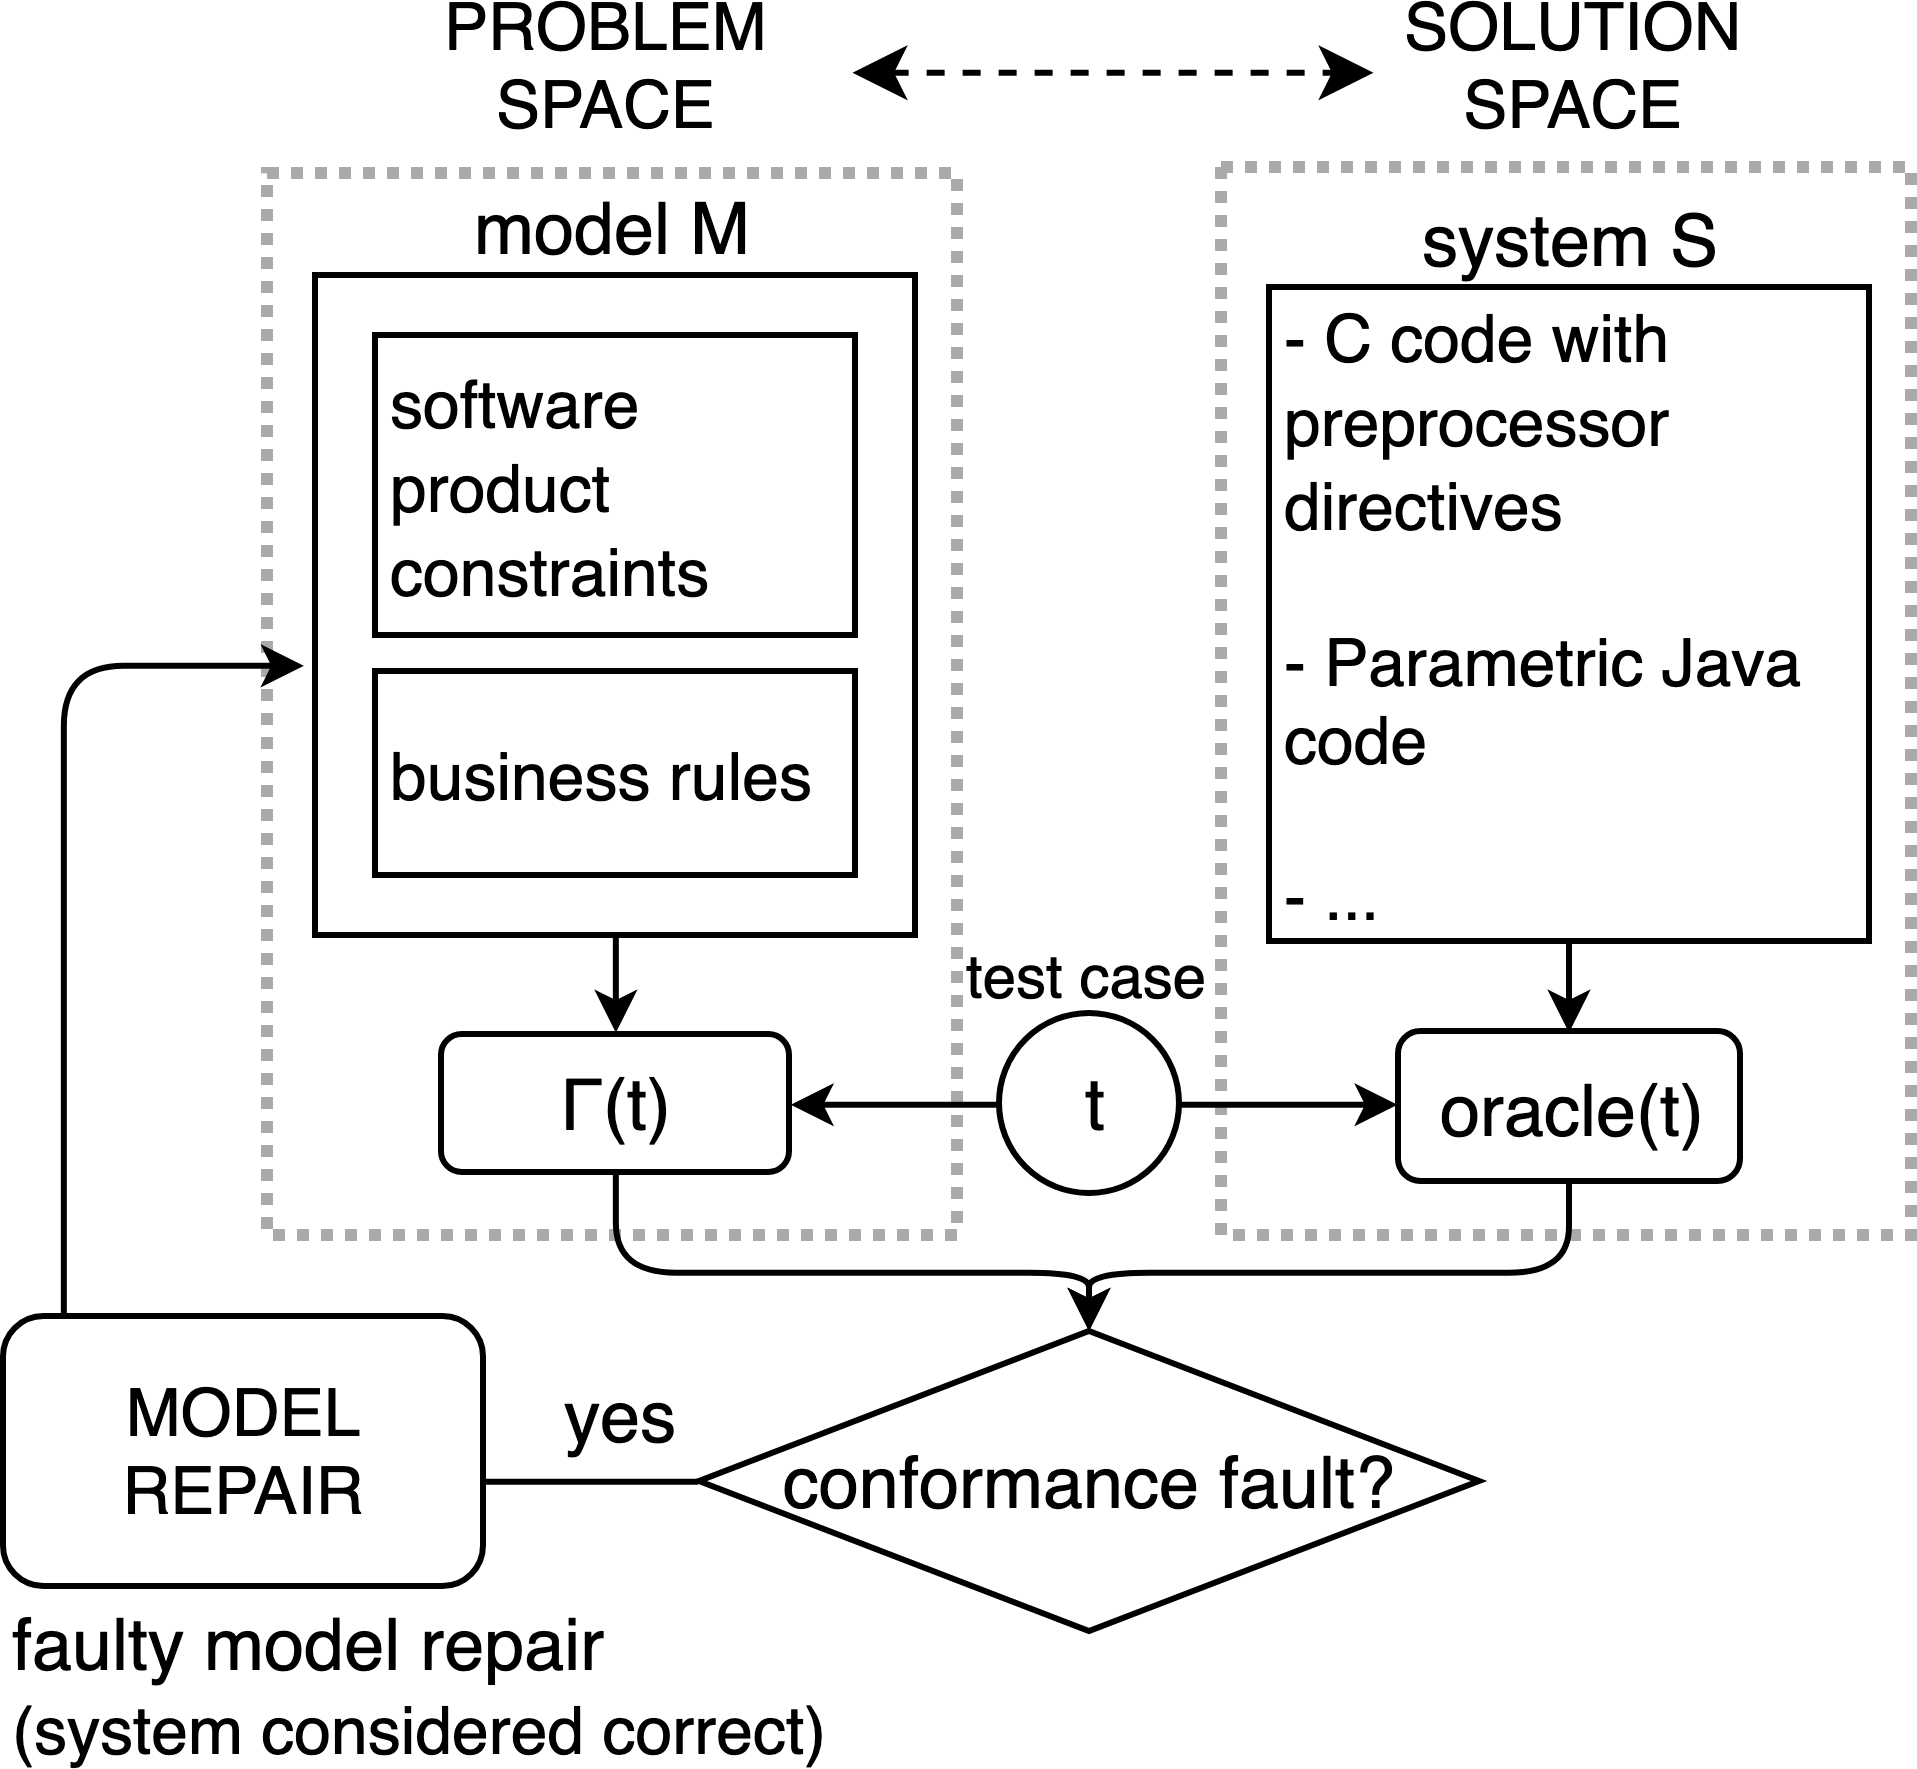
\includegraphics[width=.7\columnwidth]{images/problemSolution_new.png}
	\caption{Fault-driven repair of variability models}
	\label{fig:problem_solution}
\end{figure}

In order to detect discrepancies between the problem space and the solution space, classical techniques for testing of propositional formulas (as the constraints of a variability model) can be used: the classical decision and condition coverage, the MCDC~\cite{sej.1994.0025}, fault based criteria~\cite{compj15}, and also combinatorial testing~\cite{icst2015}. In this paper, we assume that some tests have been generated according to some coverage criterion and some \emph{faults} (i.e., non-conformances of the model w.r.t. the solution space acting as oracle) have been detected; our aim is to \emph{repair} the constraints of the variability model in order to remove the faults. We propose an automated process that, upon some failing tests, is able to \emph{automatically} correct the constraints in such a way that they maintain their original validity for all the configurations, except for those found failing.

The rest of the section reflects the content of the paper \cite{arcaini2019varivolution}, and it is organized as follows. Sect.~\ref{sec:basic} presents some basic definitions in addition to the ones introduced previously in the chapter. Sect.~\ref{sec:repair} presents the basic repair process and some possible optimizations. Sect.~\ref{sec:experiments} shows the empirical results. Threats to validity are tackled in Sect.~\ref{sec:threats}, whereas an overview of the related work is given in Sect.~\ref{sec:fmrelatedwork2}. The conclusions, together with lines for future research, are given jointly at the end of the chapter, in Sect.~\ref{sec:fmconclusions}.

\subsection{Basic Definitions}\label{sec:basic}

\begin{tikzborder}{\cite{arcaini2019varivolution}}
	\begin{mydef}[Variability Model]\label{def:varModel}
		A variability model \m is made of a set of features $F=\{f_1, \ldots, f_n\}$ and a set of constraints $\Gamma = \{\gamma_1,\ldots, \gamma_m\}$ over the features.
	\end{mydef}
	
	The features $F$ represent the system parameters. The expressions in $\Gamma$ identify the features configurations for which the actual system is expected to work.
	
	\begin{mydef}[Configuration]\label{def:configuration}
		A \emph{configuration} (or \emph{test}) $t$ is a particular assignment of values for all the features $F$. We identify with $t(f_i)$ the value of feature $f_i$ in test $t$. A configuration is {\it valid} if it respects the constraints, i.e., $t \models \Gamma$. We also use $\Gamma$ as predicate to check the constraint satisfaction: $\Gamma(t) = \true$ iff $t \models \Gamma$.
	\end{mydef}
	
	\begin{mydef}[Test suite]\label{def:testSuite}
		A \emph{test suite} \testSuite is a set of tests. We identify with \exTestSuite the \emph{exhaustive test suite}, i.e., the set of all the possible tests.
	\end{mydef}
	
	\begin{mydef}[Oracle]\label{def:oracle}
		The oracle function \oraclet tells whether the configuration $t$ is functionally correct for the system $S$.
	\end{mydef}
	
	We assume that an oracle exists, that tells whether a configuration is valid or not in the real system.
	
	We assume that the set of features $F$ is known and correctly modeled, while the constraints could be faulty.
	
	\begin{mydef}[Model correctness]\label{def:varivolution_correctness}
		We say that the model \m is \emph{correct} if it conforms with the oracle for every possible configuration $t$, i.e., $\forall t \in \exTestSuite \colon \Gamma(t) = \oraclet$. 
	\end{mydef}
	
	\begin{mydef}[Conformance fault]\label{def:conformanceFault}
		We say that the model contains a \emph{conformance fault} if there exists a configuration $t$ such that $\Gamma(t) \neq \oraclet$.
	\end{mydef}
	
	\begin{mydef}[Combination]\label{def:combination1}
		A \emph{combination} (or \emph{partial configuration}) $c$ is an assignment to a subset $\features(c)$ of all the possible features $F$, i.e., $\features(c) \subseteq F$. A configuration (or test) is thus a particular combination in which $\features(c)=F$. The value assigned by the combination $c$ to the feature $f$ is denoted as $c(f)$.
	\end{mydef}
	
	\begin{mydef}[Propositional representation of combinations]
		A combination $c$ can be expressed in propositional logic by making the conjunction of the truth value assignments of its features:
		%
		\[c = \left(\bigwedge_{\{f \in \features(c) | c(f) \}} f\right) \wedge \left(\bigwedge_{\{f \in \features(c) | \neg c(f) \}} \neg f\right)\]
	\end{mydef}
	
	\begin{mydef}[Combination containment]\label{def:combContainment1}
		A test (or configuration) $t$ \emph{contains} a combination $c$ if all features values in $c$ are the same in $t$. Formally, $\forall f_i \in \features(c) \colon c(f_i) = t(f_i)$.
		
		Given a test suite \testSuite, we identify all the tests containing a combination $c$ as $\testSuite(c)$. Formally, $\testSuite(c) = \{t \in T | c \subseteq t\}$.
	\end{mydef}
	
	\begin{mydef}[Combination completeness]\label{def:combCompl}
		Given a test suite \testSuite and a combination $c$, we say that $c$ is \emph{complete} w.r.t. \testSuite iff $\testSuite(c)$ contains all possible tests containing $c$.
	\end{mydef}
	
	
	\begin{lemma}\label{lemma:combComplLemma}
			If $c$ is complete w.r.t. a test suite \testSuite, then it holds $\forall t \in \exTestSuite \setminus \testSuite(c) \colon c = \false$.
	\end{lemma}

	\begin{mydef}[Failure-containing combination]\label{def:fcc}
		A combination $c$ is a \emph{failure-containing combination} (\fcc) if:
		%
		\begin{compactenum}
			\item $c$ is contained in at least a failing test of $~~T$, i.e., $\exists t \in \testSuite(c) \colon \Gamma(t) \neq \oraclet$.
			\item every configuration containing $c$ has the same value in the oracle, i.e., $(\forall t \in \testSuite(c) \colon \oraclet = \false) \vee (\forall t \in \testSuite(c) \colon \oraclet = \true)$. In the former case, we call $c$ an \emph{\underConstr} \fcc; in the latter case, an \emph{\overConstr} \fcc.
		\end{compactenum}
		
		We further classify a conformance fault as \emph{\underConstr fault} if it exposed by an \underConstr \fcc, or as \emph{\overConstr fault} if it is exposed by an \overConstr \fcc.
	\end{mydef}
	
	In the following, we only consider complete \fccs.\be
	
	\begin{exmp}[Under-constraining \fcc]\label{ex:example1}
		\bb Let's assume that the oracle is the system (C program) of Fig.~\ref{fig:problSolSpaces} with features $F = \{A,B,C\}$ and that we have generated the test suite shown in Table~\ref{table:underConstrFault}. Given a faulty model \mfU, with only one constraint $\Gamma = \{A\rightarrow B\}$, we observe only one fault which is represented by the \fcc $c = A \wedge \neg C$.\be
		%
		\begin{table}[!htb]
			\caption{Test suites with faults (in gray)}
			\label{table:testsandfaults1}
			\begin{subtable}[t]{.5\columnwidth}
				\centering
				\caption{\underConstr fault}
				\label{table:underConstrFault}
				\begin{tabular}{c|c|c||c|c}
					A & B & C & \mfU & oracle\\
					\hline 
					T & T & F & \cg T & \cg F\\% & \underConstr fault\\
					T & F & F & F & F\\
				\end{tabular}
			\end{subtable}%
			\begin{subtable}[t]{.5\columnwidth}
				\centering
				\caption{\overConstr fault}
				\label{table:overConstrFault}
				\begin{tabular}{c|c|c||c|c}
					A & B & C & \mfO & oracle\\
					\hline 
					F & T & T & T & T\\
					F & F & T & T & T\\
					F & T & F & \cg F & \cg T\\% & \overConstr fault\\
					F & F & F & \cg F & \cg T\\% & \overConstr fault\\
				\end{tabular}
			\end{subtable}%
		\end{table}
		%
		\bb Note that \emph{c} is a complete \fcc that identifies an \underConstr fault, i.e., it proves that the model is under-constrained. \be
	\end{exmp}
	\bb
	\begin{exmp}[Over-constraining \fcc]\label{ex:example2}
		Consider now a faulty version \mfO of the model in Fig.~\ref{fig:problSolSpaces}, characterized by $\Gamma = \{A\rightarrow B, C\}$. Given the test suite shown Table~\ref{table:overConstrFault}, we detect two \overConstr faults identified by the complete \fcc $c = \neg A$.
	\end{exmp} \be

	\subsection{Fault-driven Repair}\label{sec:repair}
		
	\bb We here propose a process to {\it repair} the constraints of a variability model, based on the detection of conformance faults between the model and the system, represented as failure-containing combinations. Fig.~\ref{fig:splrepair} shows the context in which our process is applied. \be
	%
	\begin{figure}[!ht]
		\centering
		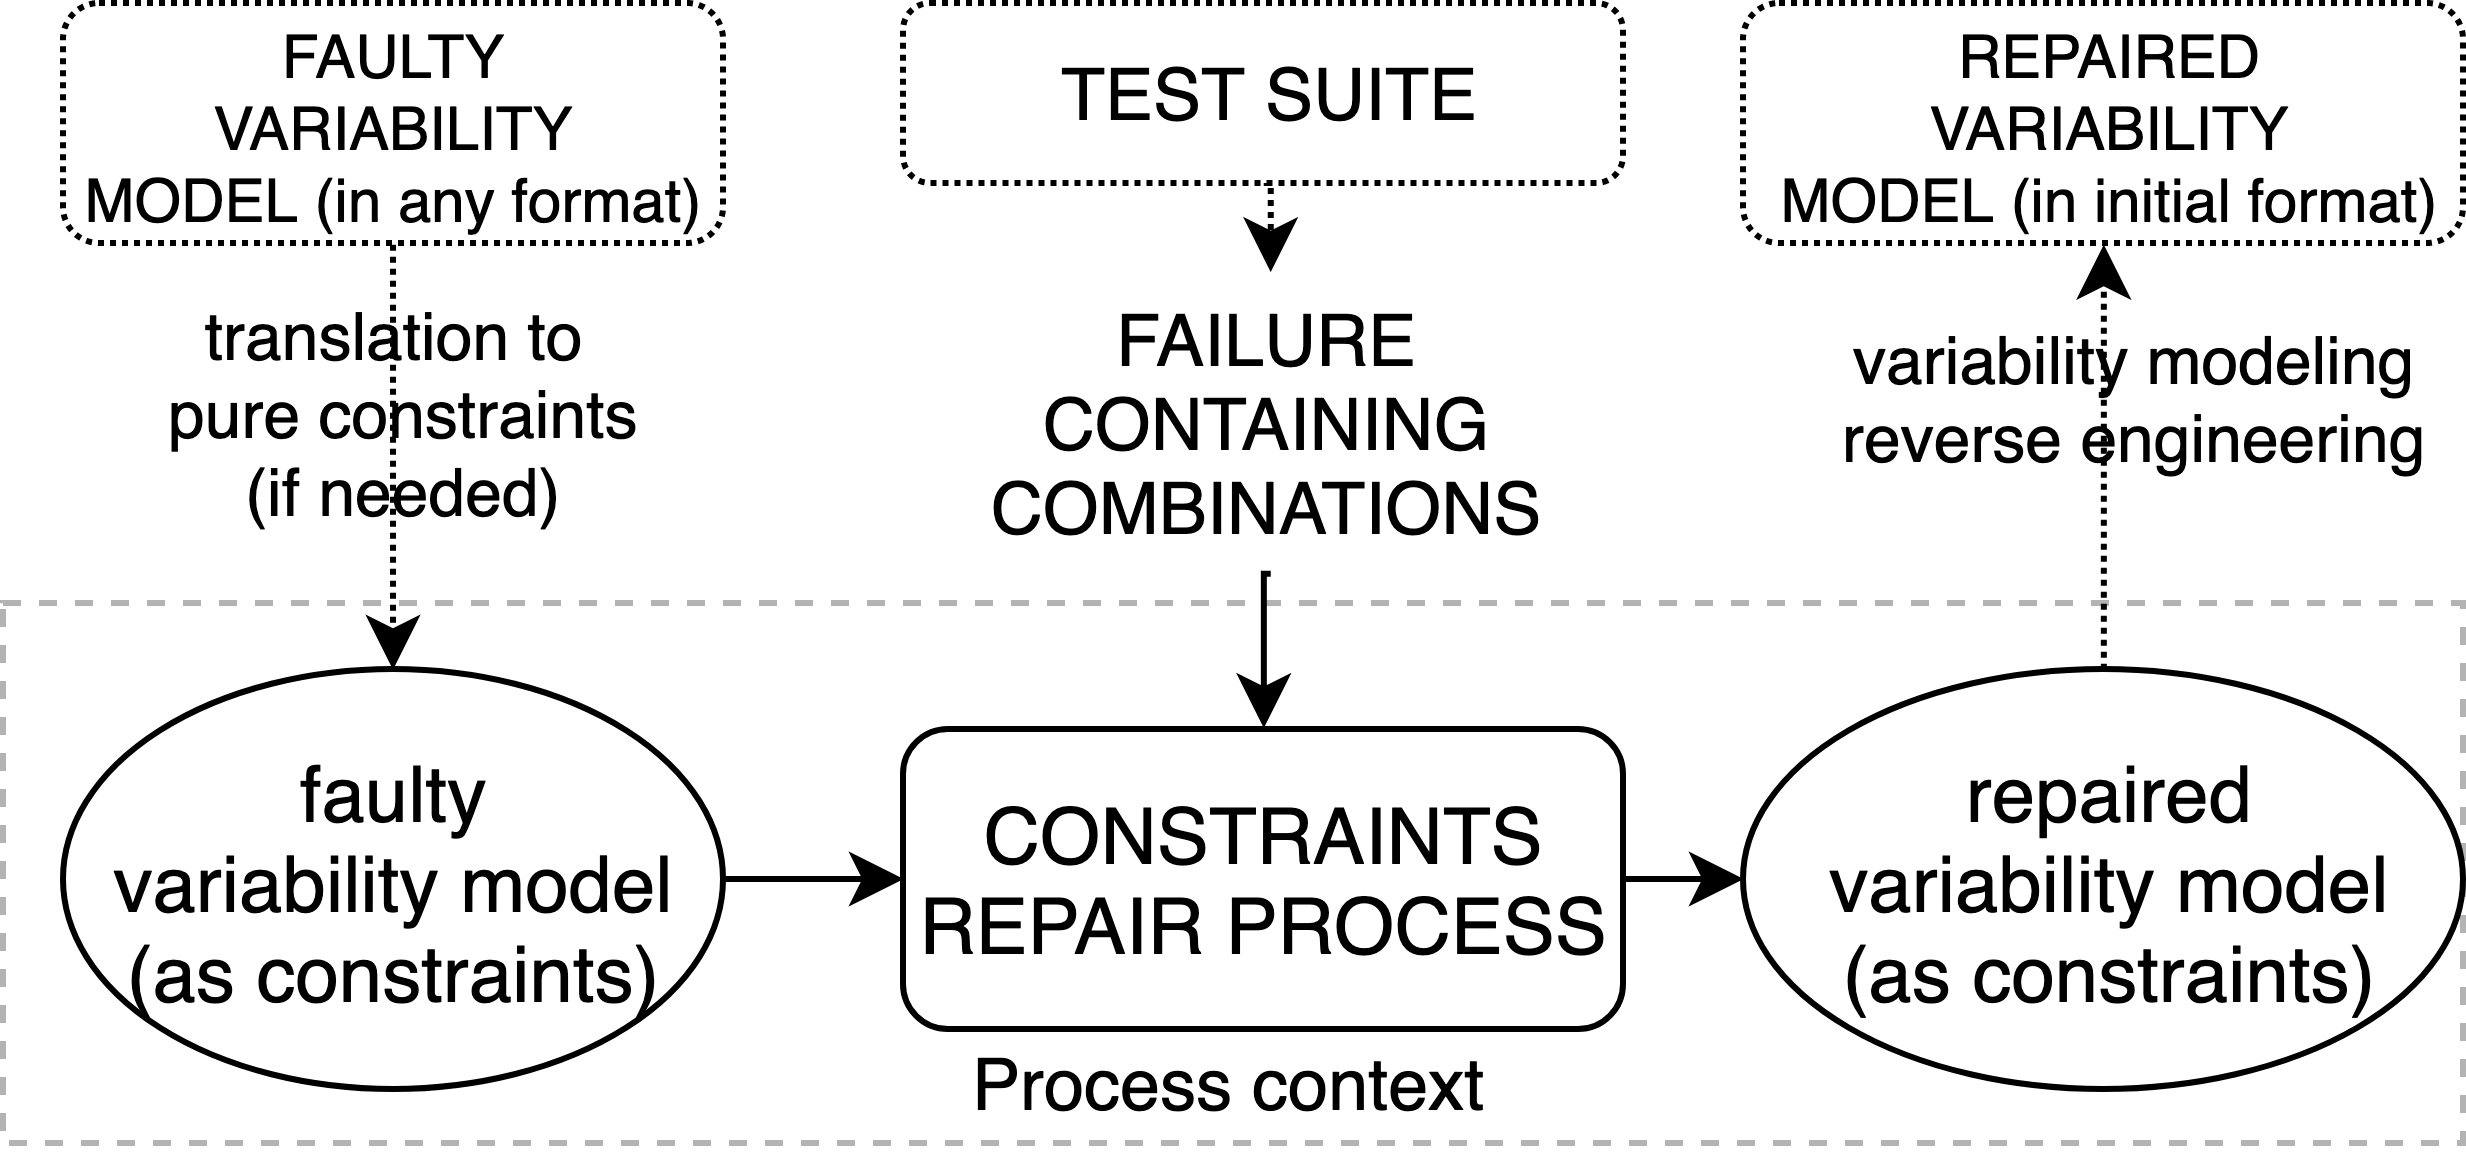
\includegraphics[width=.8\columnwidth]{images/splrepair_new.png}
		\caption{Context of the process to repair constraints among features in variability models}
		\label{fig:splrepair}
	\end{figure}
	%
	
	\bb We assume that a possibly faulty variability model is translated to a set of boolean formulas representing the constraints. For example, if the model is a feature model, semantic transformations presented in~\cite{batory2005feature} can be used. From a sufficiently large test suite, complete \fccs have been identified. To this aim, one can use well-known fault localization techniques like~\cite{ben_2015,iwct19}. Our process takes as input the \fccs and the constraints and repair them. If the user wants to go back to the initial format of the variability model, (s)he must apply some reverse engineering (which is out of the scope of this work).
	
	We first describe a na{\"i}ve implementation of the repair process in Sect.~\ref{sec:naiveAppr}, and we then introduce some optimizations in Sect.~\ref{sec:optimizedApproach}.
	\be
	
	\subsubsection{Na{\"i}ve repair approach}\label{sec:naiveAppr}
		
	\bb
	In Def.~\ref{def:fcc}, we distinguish between two types of failure-containing combinations (i.e., \underConstr and \overConstr \fcc), depending on how the model fails with respect to the oracle.
	
	We can devise a na{\"i}ve repair approach that applies a specific type of repair on the base of the fault type:
	%
	\begin{compactenum}
		\item {\tt Strengthening repair}: in case of \underConstr \fcc $c$, $\neg c$ is added as a new constraint to $\Gamma$, i.e., the constraints set $\Gamma^\prime$ of the repaired model becomes $\Gamma^\prime: = \Gamma \cup \{\neg c\}$.
		\item {\tt Weakening repair}: in case of \overConstr \fcc $c$, $c$ is disjuncted with every constraint in $\Gamma$, i.e., the constraints set $\Gamma^\prime$ of the repaired model becomes $\Gamma^\prime = \cup_{\gamma_i \in \Gamma}\{ \gamma_i \vee c\}$.
	\end{compactenum}
	
	
	\begin{exmp}[Strengthening repair]\label{ex:example_rep1}
		The \textit{\underConstr} fault in Ex.~\ref{ex:example1} is repaired by adding $\neg c = \neg(A\wedge\neg C) \equiv A \rightarrow C$ as a new constraint in $\Gamma$. The repaired constraints become $\Gamma^\prime = \{A\rightarrow B, A\rightarrow C\}$.
	\end{exmp}
	
	
	\begin{exmp}[Weakening repair]\label{ex:example_rep2}
		The \textit{\overConstr fault} in Ex.~\ref{ex:example1} is repaired by adding $c = \neg A$ in disjunction with all the existing constraints, so that the repaired constraints become $\Gamma^\prime = \{(A \rightarrow B) \vee \neg A, C \vee\neg A\}$. Note that the first constraint is {\it redundant}, as it is equivalent to the original constraint $A \rightarrow B$. The only necessary application of the repair is the one in the second constraint, as it correctly allows to have both features $A$ and $C$ assigned to {\it false} (as in the oracle).
	\end{exmp}
	
	
	
	
	\begin{thm}[Correctness of the na{\"i}ve approach]\label{thm:correctnessNaive}
		If a combination $c$ is complete w.r.t. its test suite $\testSuite(c)$, the repairs applied by the na{\"i}ve approach to $\Gamma$ (obtaining the modified constraints set $\Gamma ^\prime$) are {\it correct}, i.e., they remove all existing faults in $\testSuite(c)$ and do not introduce new ones, i.e.,
		%
		\begin{compactenum}
			\item $\forall t \in \testSuite(c) \colon \Gamma^\prime(t) = \oracle(t)$;
			\item $\forall t \in \exTestSuite \setminus \testSuite(c) \colon \Gamma^\prime(t) = \Gamma(t)$.
		\end{compactenum}
	\end{thm}
	
	\begin{proof}
		Let's consider the two kinds of repairs separately:
		%
		\begin{compactitem}
			\item {\tt Strengthening repair}: the repaired constraints are $\Gamma^\prime = \{\gamma_1, \dots, \gamma_m, \gamma_{m+1}\}$, where $\gamma_{m+1} = \neg c$.
			%
			\begin{compactenum}
				%
				\item From the definition of \underConstr \fcc, we know that it holds $\forall t \in \testSuite(c) \colon \oraclet = \false$. Furthermore, we also know that $\forall t \in \testSuite(c) \colon \Gamma^\prime(t) = \false$, because the new constraint $\gamma_{m+1} = \neg c$ falsifies all the tests containing the \fcc $c$. Therefore, it holds $\forall t \in \testSuite(c) \colon \Gamma^\prime(t) = \oraclet$.
				\item
				By Lemma~\ref{lemma:combComplLemma}, we know that $\forall t \in \exTestSuite \setminus \testSuite(c) \colon c = \false$.
				Therefore, the added constraint $\gamma_{m+1} = \neg c$ is always true in tests $\exTestSuite \setminus \testSuite(c)$. Since $\gamma_{m+1}$ has no influence on the evaluation of these tests, it holds $\forall t \in \exTestSuite \setminus \testSuite(c) \colon \Gamma^\prime(t) = \Gamma(t)$.
			\end{compactenum}
			\item {\tt Weakening repair}: the repaired constraints are $\Gamma^\prime = \{ \gamma_1 \vee c, \dots, \gamma_m \vee c\}$.
			%
			\begin{compactenum}
				\item From the definition of \overConstr \fcc, we know that it holds $\forall t \in \testSuite(c) \colon \oraclet = \true$.
				Furthermore, we also know that $\forall t \in \testSuite(c) \colon \Gamma^\prime(t) = \true$, because all the constraints $\gamma_i^\prime = \gamma_i \vee c$ admit all the tests containing the \fcc $c$. Therefore, $\forall t \in \testSuite(c) \colon \Gamma^\prime(t) = \oraclet$.
				\item
				By Lemma~\ref{lemma:combComplLemma}, we know that $\forall t \in \exTestSuite \setminus \testSuite(c) \colon c = \false$. Since $c$ is added as a disjunction to the existing constraints, it leaves the constraints equivalent to the original ones, i.e., $\forall t \in \exTestSuite \setminus \testSuite(c) \colon \Gamma^\prime(t) = \Gamma(t)$.
			\end{compactenum}
		\end{compactitem}
	\end{proof}
	\be

	\subsubsection{Optimized repair approach}\label{sec:optimizedApproach}
		
	\bb The na{\"i}ve repair approach described in Sect.~\ref{sec:naiveAppr} could generate some redundancy, as shown in Ex.~\ref{ex:example_rep2}. Therefore, we introduce techniques for constraint selection and simplification to reduce the potential redundancy generated by the na{\"i}ve approach. The goal is to make fewer edits as possible to the model, since we assume that a model with fewer edits better preserves domain knowledge.
	
	Fig.~\ref{fig:repair_process} shows the optimized repair approach.\be
	%
	\begin{figure*}[!ht]
		\centering
		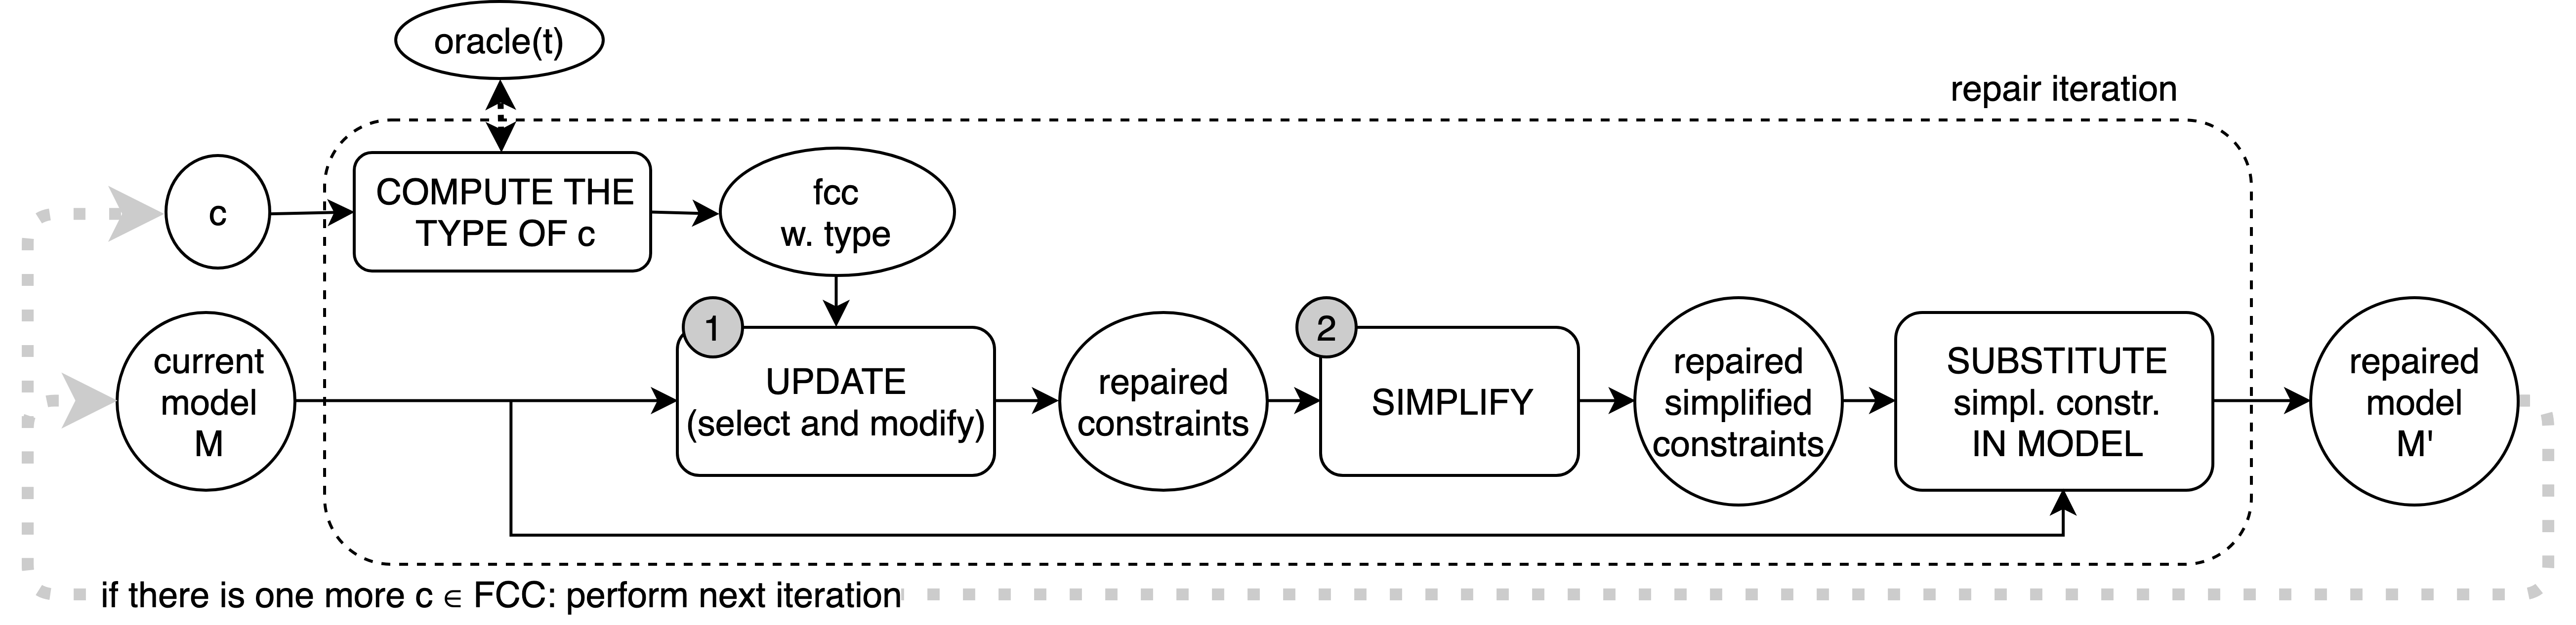
\includegraphics[width=1\textwidth]{images/repair_process_new.png}
		\caption{Single iteration of the optimized repair approach}
		\label{fig:repair_process}
	\end{figure*}
	%

	\bb It consists of three phases:
	%
	\begin{inparaenum}[(1)]
		\item \textsf{selection} of some constraints to modify,
		\item \textsf{modification} of the selected constraints, and
		\item \textsf{simplification} of the modified constraints.
	\end{inparaenum}
	%
	Note that the process can be iterative if we identified more than one \fcc (as in the experiments in Sect.~\ref{sec:repairevaluation}). In the following, we consider one iteration of the process.\be
	
	\subsubsection{Update phase: \textsf{selection} and \textsf{modification}}\label{sec:selectionAndMod}
	\bb To preserve the domain knowledge embedded in the constraints, we want the process to make as few changes as possible to them. Namely, we would like that the constraints $\Gamma$ are updated with the following qualities:
	%
	\begin{compactenum}
		\item possibly no more constraints are added;
		\item as many constraints as possible are preserved identical;
		\item some constraints can be removed.
	\end{compactenum} 
	%
	Therefore, the process performs a pre-processing phase, which selects only the constraints $\Gamma_S \subseteq \Gamma$ containing some configurations in common with the \fcc $c$, and then modifies them. This phase is specific to the type of repair:
	%
	\begin{compactitem}
		\item[\textbf{Strengthening repair}] Only the constraints $\gamma_i$ sharing at least one feature with the \fcc $c$, are selected. Formally, $\Gamma_S = \{\gamma_i \in \Gamma | (\features(\gamma_i) \cap \features(c)) \neq \emptyset\}$, where \features collects the features contained in a formula. Then, the modification phase updates only one constraint $\gamma_s$ selected randomly from $\Gamma_S$, by conjuncting $\neg c$. The repaired constraints set becomes $\Gamma^\prime = (\Gamma \setminus \{\gamma_s\}) \cup \{\gamma_s \wedge \neg c\}$.
		\item[\textbf{Weakening repair}] Only the constraints $\gamma_i$ that exclude at least one configuration contained in the \fcc $c$ are selected. Formally, $\Gamma_S = \{\gamma_i \in \Gamma | \sat(\neg \gamma_i \wedge c )=\true\}$, where \sat tells whether a formula is satisfiable or not. Then, the modification phase updates all the constraints in $\Gamma_S$ by disjuncting them with $c$. The repaired constraints set becomes $\Gamma^\prime = (\Gamma \setminus \Gamma_s) \cup \bigcup_{\gamma_i \in \Gamma_s} \{\gamma_i \vee c\}$.
	\end{compactitem}\be
	
	\subsubsection{\textsf{Simplification} phase}\label{sec:simplification}
	\bb The constraint \textsf{simplification} procedure aims at reducing redundancy in the repaired model, especially when failure-containing combinations involve many features. A straightforward way to simplify a formula (or make it more readable) is to find the smallest, but equivalent expression. This problem is known as the \textit{minimum-equivalent-expression} problem~\cite{Buchfuhrer:2011:CBF:1889388.1889508, hemaspaandra_minimization_2011}.
	
	We compared the three existing formula minimization techniques, and one minimization method based on mutations we have implemented (\atgt):
	%
	\begin{compactenum}
		\item \jbool\footnote{JBool: \url{https://github.com/bpodgursky/jbool_expressions}}: a tool that recursively applies logic rules and preprocessing techniques, preserving equivalence~\cite{Biere2012}: \textit{literal removal}, \textit{negation simplification}, \textit{and/or reduplication and flattening}, \textit{child expression simplification}, \textit{and propagation}, \textit{De Morgan's law}.
		\item \textsf{Quine-McCluskey} (\qm)~\cite{Quine3}, a generalization of the Karnaugh Maps method. It requires the constraints to be in Disjunctive Normal Form (DNF) and its exponential complexity in the number of features makes it suitable only for small models (up to 15 features).
		\item \espresso\footnote{Espresso logic minimizer, sources available at \url{https://ptolemy.berkeley.edu/projects/embedded/pubs/downloads/espresso/index.htm}}, a faster version of the \qm method that relies on some heuristics~\cite{Rudell:M86/65}.
		\item \atgt\footnote{ATGT: ASM Test Generation Tool. \url{http://fmse.di.unimi.it/atgtBoolean.html}}~\cite{CalvagnaG09}: a hill-climbing process we implemented that iteratively mutates a formula randomly and checks it for equivalence. %(\red{see removing vacuus constraints}).
	\end{compactenum}
	
	We propose different methods, as we have seen that, in practice, these techniques often produce different outputs and none of them is guaranteed to generate an output which is always minimal compared to the others.\be

	\subsubsection{Correctness}
	
	\bb Does the optimized approach produce correct repairs? A repair $r$ is correct if it is equivalent to the one obtained by the na{\"i}ve approach.
	
	\begin{thm}[Correctness of the optimized approach]\label{thm:correctnessOptmised}
		The optimized approach is correct.
	\end{thm}
	
	\begin{proof}
		The techniques applied in the \emph{simplification phase} preserve equivalence. Therefore, we only show that the repairs computed in the \emph{update phase} are equivalent to those computed by the na{\"i}ve approach, because the two following properties hold:
		%
		\begin{compactitem}
			\item The strengthening repair is correct because of distributivity and commutativity of boolean conjunction: $\gamma_1 \wedge \ldots \wedge \gamma_s \wedge \ldots \wedge \gamma_m \wedge \neg c \equiv \gamma_1 \wedge \ldots \wedge (\gamma_s \wedge \neg c) \wedge \ldots \wedge \gamma_m$.
			\item The weakening repair is by definition equivalent to the na{\"i}ve approach for all the constraints $\gamma_i$ that are selected in $\Gamma_S$ to be modified in the optimised approach (i.e., it performs the same operation of the na{\"i}ve approach). It is correct also for each non-selected constraints $\gamma_j$, since for these constraints it holds $\gamma_j \vee c = \gamma_j$ (as $c$ is \false in the non-selected constraints): thus, $\gamma_j$ can be left as it is. In fact, by translating this expression to a satisfiability problem, we obtain the condition under which the process does not select the constraint:
			%
			\begin{align*}
			((\gamma_j \vee c) = \gamma_j) &\Leftrightarrow \neg \sat((\gamma_j \vee c) \neq \gamma_j) \\
			& \Leftrightarrow \neg \sat( (\gamma_j \vee c) \oplus \gamma_j) \\
			& \Leftrightarrow \neg \sat( (\gamma_j \wedge \neg \gamma_j) \vee (c \wedge \neg \gamma_j) \vee (\neg \gamma_j \wedge \neg c \wedge \gamma_j) ) \\
			& \Leftrightarrow \neg \sat(\neg \gamma_j \wedge c) \\
			\end{align*}
		\end{compactitem}
	\end{proof}\be

	\subsection{Evaluation}\label{sec:repairevaluation}
		
	\bb In order to apply our process, we need a faulty variability model \m, a set of failure-containing combinations \fccSet, and an {\it oracle}. For the sake of experiments, we take as oracle another variability model \mO, instead of the real oracle; in this way, we can also extract the set \fccSet by comparing \m and \mO. \be

	\subsubsection{Benchmarks}
		
	\bb We have built two sets of benchmarks: \benchMut with seeded faults, and \benchReal with versioned models.\be
	
	\paragraph{\benchMut (seeded faults)} 
	\bb In order to build this benchmark set, we first selected some models to be used as \mO, from previous papers and feature model repositories:
	%
	\begin{compactitem}
		\item \exampleM, from Example~\ref{ex:example1}.
		\item \register, a VSpec model for a register typically found in supermarkets, inspired by~\cite{Shimbara2015}.
		\item \django, an open source web application framework written in Python. Each Django project has a configuration file loaded at launch time. We considered 12 Boolean parameters (features), with constraints devised in our previous work~\cite{gargantini_combinatorial_2017}.
		\item \textsf{tight\_vnc} from FeatureIDE repository~\cite{FeatureIDEbook}.
	\end{compactitem}
	%
	In order to obtain the initial faulty model \m, we seeded random faults in \mO using the following mutation operators:
	%
	\begin{compactitem}
		\item \textbf{\textsf{RC}}: removal of a constraint. There are studies showing that this is the most common case in practice~\cite{lotufo_evolution_2010}.
		\item \textbf{\textsf{RL}}: removal of a literal in a constraint.
		\item \textbf{\textsf{SL}}: substitution of a literal in a constraint.
	\end{compactitem}
	
	We generated 30 faulty versions \m of each model \mO (10 with each mutation operator).\be 
	
	\paragraph{\benchReal (versioned models)}
	\bb For this benchmark set, we have considered two versions of variability models of the same system. We use the second version as oracle \mO, and the first one as the faulty model \m. We picked three models of industrial applications from the SPLOT repository\footnote{\url{http://52.32.1.180:8080/SPLOT/feature_model_repository.html}}~\cite{mendonca2009splot}:
	%
	\begin{compactitem}
		\item the process model \rhiscom, between versions 2.0 and 3.0;
		\item an enterprise resource planner (\erpSpl);
		\item a \windows accessibility module, between versions 7.0 and 8.0.
	\end{compactitem}
	
	
	Table~\ref{table:benchs} reports the size of all the faulty models \m to be repaired in the two benchmarks, in terms of number of features, number of constraints, and total number of literals in the constraints.\be 
	%
	\begin{table}[!htb]
		\centering
		\caption{Benchmarks size}
		\label{table:benchs}
		%\resizebox{\columnwidth}{!}{
		\begin{tabular}{clrrr}
			\toprule
			& Name & \# features & \# constraints & \# literals\\
			&    &      & avg(min - max)\\
			\midrule
			\multirow{4}*{\rotatebox{90}{\small \benchMut}}
			&\exampleM & 3 & 1.67 (1-2) & 3.0 (2-4) \\
			&\register & 3 & 1.67 (1-2) & 3.87 (2-5) \\
			&\django & 12 & 4.6 (4-5) & 10.87 (9-12) \\
			&\tightVnc & 24 & 11.67 (11-12) & 53.2 (45-55) \\
			\midrule
			\multirow{3}*{\rotatebox{90}{\small \benchReal}}
			&\rhiscom & 36 & 70 & 140 \\
			&\erpSpl & 43 & 75 & 151 \\
			&\windows & 335 & 943 & 2031 \\
			\bottomrule
		\end{tabular}%}
	\end{table}
	%
\bb 	For the constraints and literals of \benchMut, it reports the average number across the 30 mutants and the minimum and maximum number between parentheses (the number of features is the same across the mutants).\be
	
	\subsubsection{Failure-containing combinations}
		
	\bb For the sake of experiments, we obtain the set \fccSet from the faulty model \m (having constraints $\Gamma$) and the model we use as oracle \mO (having constraints $\Gamma_o$), using the following process:
	%
	\begin{compactenum}
		\item first, we generate a test showing the difference (i.e., conformance fault) between the two models. The test is built as $t = \mathit{getModel}(\Gamma \neq \Gamma_o)$, where $\mathit{getModel}$ returns a model of the propositional expression, if it exists, or $\mathit{null}$ (in this case, the models are equivalent).
		\item then, we start from $c \leftarrow t$, and,
		\begin{compactitem}
			\item if $\Gamma_o(t)$, for each feature $f \in F$, if $\neg \sat(\neg \Gamma_o \wedge \mathit{rem}(f, c))$ holds, then we do $c \leftarrow \mathit{rem}(f, c)$, where $\mathit{rem}$ removes the assignment of $f$ in $c$ and returns the modified $c$.
			\item if $\neg \Gamma_o(t)$, for each feature $f \in F$, if $\neg \sat(\Gamma_o \wedge \mathit{rem}(f, c))$ holds, then we do $c \leftarrow \mathit{rem}(f, c)$.
		\end{compactitem}
	\end{compactenum}
	%
	This way we can obtain \fccs that are as minimal as possible, and complete (i.e., the oracle is always true in case of \overConstr \fcc, and always false in case of an \underConstr \fcc).\be
	
	\subsubsection{Repair quality metrics}\label{sec:qualityMetrics}
		
	\bb We want to assess the quality of a repair w.r.t. two goals:
	%
	\begin{inparaenum}[(i)]
		\item simplification of the constraints, and
		\item minimization of the impact of edits.
	\end{inparaenum}
	%
	To this aim, we introduce two quality metrics that are used to compare Boolean expressions. We apply them to compare the conjunction of the constraints $\Gamma$ of the original model \m and the constraints $\Gamma^\prime$ of the repaired model \mRep obtained as output of the approach. The metrics are defined as follows:
	%
	\begin{compactitem}
		\item{Complexity Distance (\textsf{CD})} as difference of formula sizes $\mathit{CD}(\Gamma, \Gamma^\prime) = \mathit{literals}(\Gamma) - \mathit{literals}(\Gamma^\prime)$, where $\mathit{literals}$ returns the number of literals in a formula. As in~\cite{vonRhein2015}, we also considered other measures (number of operators and node count in the parsed tree representation), but they do not change the overall results, therefore we do not report them here.
		\item {Edit Distance (\textsf{ED})} computed between the syntactic trees of the two formulas $\Gamma$ and $\Gamma^\prime$. $\mathit{ED}(\Gamma, \Gamma^\prime)$ is defined as the number of {\it edits} (addition, substitution, or elimination) that we have to apply to $\Gamma$ in order to obtain $\Gamma^\prime$. A node of the tree can either be a literal or an operator. We use \textsf{APTED} as a tool to efficiently compute tree edit distances~\cite{pawlik_tree_2016}.
	\end{compactitem}
\be

	\subsubsection{Experiments}\label{sec:evaluation}
		
	\bb We run experiments on the two benchmark sets \benchMut and \benchReal: namely, we applied the na{\"i}ve approach (see Sect.~\ref{sec:naiveAppr}), the optimized approach (see Sect.~\ref{sec:optimizedApproach}) without the \textsf{simplification} phase (\textsf{\onlySelection}), and with the \textsf{simplification} phase (employing the \atgt, \espresso, \jbool and \qm methods). Experiment code was written in Java and experiments were executed on a Linux PC with Intel(R) i7-3770 CPU (3.4 GHz) and 16 GB of RAM. All reported results are the average of 10 runs with a timeout for a single repair of 1 hour. The code and the benchmarks are available at \url{https://github.com/fmselab/VMConstraintsRepair}.
	
	Results of the experiments are reported in Table~\ref{tab:experimentb}.\be
	%
	\begin{table*}[!hbt]
		\caption{Experimental results {(mut.: mutation type; s.: strengthening repairs; w.: weakening repairs; ED: edit distance; CD: complexity distance; t: time in milliseconds, T/O: timeout occurred). In gray the best results (CD and ED over all the approaches, time over the simplification approaches)}}
		\label{tab:experimentb}
		\resizebox{\textwidth}{!}{%
			\centering%\small
			\setlength\tabcolsep{2pt} 
			\begin{tabular}{ccc|cc|ccc|ccc|ccc|ccc|ccc|ccc}
				\toprule
				& & & \multicolumn{2}{c|}{\fccs and repairs} & \multicolumn{3}{c|}{Na{\"i}ve} & \multicolumn{3}{c|}{\onlySelection} &\multicolumn{12}{c}{simplification} \\
				\cline{12-23}
				& & &&&& & & & & &\multicolumn{3}{c}{\atgt} & \multicolumn{3}{c}{\espresso} & \multicolumn{3}{c}{\jbool} & \multicolumn{3}{c}{\qm}\\
				& name & mut. & \# (s.+w.) & size (s./w.) & CD & ED & t & CD & ED & t & CD & ED & t & CD & ED & t & CD & ED & t & CD & ED & t \\ 
				\midrule
				\multirow{12}*{\rotatebox{90}{\small \benchMut}}
				& \multirow{3}{*}{\exampleM} & RC & 1.0+0.0 &2.0 / -- & 2.0 & 5.0 & 0.1 & 2.0 & 5.0 & 0.4 & 2.0 & 5.0 & 1064 & 2.0 & 5.0 & 53.4 & 2.0 & \cg 4.0 & \cg 5.3 & 2.0 & \cg 4.0 & 24.2 \\
				& & RL & 0.3+1.0 & 2.0 / 1.0 & 3.8 & 10.8 & 0.2 & 2.2 & 6.0 & 0.3 & 2.2 & 6.0 & 1371 & 2.2 & 6.0 & 68.2 & \cg 1.6 & \cg 4.2 & \cg 1.0 & \cg 1.6 & \cg 4.2 & 30.9 \\
				& & SL & 0.5+0.3 & 2.0 / 1.0 & 1.2 & 3.2 & 0.0 & \cg 1.0 & \cg 2.6 & 0.0 & \cg 1.0 & \cg 2.6 & 1060 & \cg 1.0 & 3.0 & 52.4 & \cg 1.0 & \cg 2.6 & \cg 1.1 & \cg 1.0 & \cg 2.6 & 23.3 \\\\[-.2cm]
				& \multirow{3}{*}{\register} & RC & 1.0+0.0 & 2.6 / -- & 2.3 & 5.6 & 0.0 & 2.3 & 5.6 & 0.3 & 2.3 & 5.6 & 1065 & 2.3 & 5.6 & 52.4 & 2.3 & \cg4.9 & \cg1.0 & 2.3 & \cg4.9 & 24.0 \\
				& & RL & 0.2+1.1 & 2.6 / 1.3 & 5.5 & 14.6 & 0.0 & 2.9 & 7.7 & 0.3 & 2.5 & 6.9 & 1388 & 2.9 & 8.5 & 68.1 & \cg2.2 & \cg6.6 & \cg0.6 &\cg 2.2 & \cg6.6 & 30.8 \\
				& & SL & 0.9+0.3 & 2.1 / 1.4 & 2.9 & 7.4 & 0.2 & \cg 2.1 & \cg5.2 & 0.2 & \cg 2.1 & \cg5.2 & 1433 & \cg2.1 & 6.0 & 69.2 & \cg2.1 & 5.7 & \cg1.2 & \cg2.1 & 5.7 & 32.9 \\\\[-.2cm]
				& \multirow{3}{*}{\django} & RC & 0.5+0.0 & 1.7 / -- & 0.8 & 2.2 & 0.0 & 0.8 & 2.2 & 0.0 & 0.8 & 2.2 & 1062 & 0.8 & 2.2 & 52.2 & 0.8 & \cg1.3 & \cg1.0 & 0.8 & \cg1.3 & 24.2 \\
				& & RL & 0.4+1.4 & 2.0 / 4.0 & 8.0 & 22.8 & 0.0 & 1.6 & 4.4 & 0.6 & \cg1.2 & 3.2 & 2424 & 1.6 & 4.4 & 119.9 & \cg1.2 & \cg3.0 & \cg2.5 & \cg1.2 & 3.2 & 58.1 \\
				& & SL & 0.8+2.3 & 1.0 / 4.0 & 33.3 & 94.4 & 0.0 & 6.5 & 18.3 & 2.1 & \cg5.8 & \cg16.6 & 3720 & 6.5 & 19.2 & 180.3 & 7.4 & 21.7 & \cg4.2 & \cg5.8 & 18.4 & 116.0 \\\\[-.2cm]
				
				& \multirow{3}{*}{\tightVnc} & RC & 4.7+0.0 & 2.7 / -- & 14.0 & 39.1 & 0.1 & 14.0 & 39.1 & 11.0 & 14.0 & 39.1 & 8252 & 14.0 & 39.1 & 267 & 14.0 & \cg27.1 & \cg23.5 & 14.0 & 39.6 & 11199 \\
				& & RL & 0.7+31.8 & 1.9 / 14.2 & 2422 & 6000 & 1.2 & 202.2 & 499.5 & 402 & -- & -- & T/O & 202.2 & 499.5 & 2275 & -- & -- & T/O & -- & -- & T/O \\
				& & SL & 1.5+18.5 & 4.1 / 11.2 & 3734 & 8860 & 0.7 & 244.0 & 585.8 & 165 & -- & -- & T/O & 244.0 & 585.8 & 1369 & -- & -- & T/O & -- & -- & T/O \\
				
				\midrule
				\multirow{3}*{\rotatebox{90}{\small \benchReal}}
				& \rhiscom & -- & 9+6 & 1.2 / 35.3 & 13977 & 30634 & 2 & 197 & \cg504 & 128 & -- & -- & T/O & 197 & 511 & 2717 & -- & -- & T/O & -- & -- & T/O \\
				& \erpSpl & -- & 9+232 & 2.0 / 37.1 & 723426 & 1604116 & 15 & 16562 & 37273 & 8555 & -- & -- & T/O & 16562 & 37273 & 16562 & -- & -- & T/O & -- & -- & T/O \\
				& \windows & -- & 989+55 & 2.3 / 453.8 & 8537492 & 17028426 & 87 & 175380 & 1918927 & 114028 & -- & -- & T/O & \cg174200 & \cg 1917875 & 245532 & -- & -- & T/O & -- & -- & T/O \\
				\bottomrule
			\end{tabular}
		}
	\end{table*}
	%
	
\bb 	For benchmarks \benchMut, results are categorized by the type of mutation. For each benchmark model, the table reports the number and size of strengthening and weakening repairs (note that each repair corresponds to one \fcc); moreover, for each process setting, it reports the execution time, and the quality of the final model \mRep in terms of $\mathit{CD}$ and $\mathit{ED}$ distances. Values of the strategies \atgt, \jbool and \qm for repairing \textsf{RL} and \textsf{SL} mutations of \tightVnc and for all the benchmarks of \benchReal are not reported, because the experiment exceeded the timeout (T/O) of 1 hour.
	
	We evaluate the process using three research questions.
	
	\researchquestion{Which quality do the constraints repaired by the process have?}
	
	The main goal of this repair process is to not destroy domain knowledge. We consider the quality measures \textsf{ED} and \textsf{CD} to be proxies for domain knowledge preservation, under the assumption that having fewer edits means more preservation of the domain knowledge contained in the constraints. We therefore consider an approach {\it better} than another approach if it has smaller values of the quality measures.
	
	The process (in all its versions) completely repairs all the benchmarks models, as the \fccs in \fccSet are complete (see Thms.~\ref{thm:correctnessNaive} and \ref{thm:correctnessOptmised}). However, the quality of the repaired models depends on the adopted repair approach. The optimized approach only using selection (\onlySelection) always outperforms the na{\"i}ve process in terms of quality of the repairs, as it modifies a subset of the constraints, and so the two measures CD and ED for it are always lower. The simplification approaches sometimes allow to obtain better repairs than \onlySelection, meaning that they remove some redundancy introduced by the repair; however, there is no simplification method that is always better than the others on all the benchmarks for both measures (except for \atgt that is never worse than \espresso). 
	We observe that, in a few cases, CD and ED are higher for a simplification method w.r.t. \onlySelection (e.g., ED of \espresso for \register RL): we have checked the example and we found that the simplification has removed some redundancy that was already present in the original model \m so modifying the model more than what done by \onlySelection.
	
	
	\researchquestion{How efficient is the repair approach?}
	
	Computational time varies significantly for the different approaches and models: from 0-0.1ms of the smallest models, up to 245 seconds for the \windows model (the biggest model having 335 features and 943 constraints) repaired with the \espresso simplifier.
	
	The na{\"i}ve approach, and the optimized approach without simplification (\onlySelection), have been the fastest approaches; execution times of \onlySelection are higher than the na{\"i}ve approach for big models, as it uses a SAT solver for identifying the constraints that must be repaired (see Sect.~\ref{sec:selectionAndMod}). Simplification algorithms are the main responsible for slow performance in terms of computation time. \atgt is the slowest one, as it internally calls a SAT solver several times, and the algorithm is yet in a prototypical stage. The second slowest simplification method is \espresso, but we noticed that it is relatively faster than other methods for large models; indeed, it is the only approach able to simplify all the benchmark models, while the others cannot simplify the biggest mutations obtained for \tightVnc and all the models in \benchReal in the given timeout. For small models, \jbool is the fastest simplification method, followed by \qm; however, they both timeout for large models.
	
	
	
	\researchquestion{Is there a repair type that our process handles more efficiently?}
	We are here interested in investigating whether there is an effect of the type of repair on the performances of the process. In order to better understand the computational cost of the type of repairs, Table~\ref{tab:experimentc} reports, for \benchReal, the average execution times of strengthening and weakening repairs in the selection and simplification phases, and also the average time of any repair (regardless of the type).\be
	%
	\begin{table}[!hbt]
		\centering%\small
		\caption{Detailed results of the execution time for \benchReal}
		\label{tab:experimentc}
		%\resizebox{\columnwidth}{!}
	\end{table}
	%
	
	\bb We only report the results of \espresso, as it is the only tool that completes before the timeout of 1 hour.
	
	We observe that, in the selection phase, strengthening repairs are faster than weakening repairs: indeed, the former ones only do a syntactical analysis of the constraint, while the latter ones need to call a SAT solver (see Sect.~\ref{sec:selectionAndMod}). The average repair time in the selection phase is then influenced by the number of repairs of the two types: in \erpSpl, since almost all the repairs are weakening (see Table~\ref{tab:experimentb}), the average time is mostly influenced by them; in \windows, instead, most of the repairs are strengthening (see Table~\ref{tab:experimentb}) and so the average repair time is influenced by them.
	
	Regarding the simplification phase, there is no significant difference between the two types of repairs.\be 
	
	\subsection{Threats to Validity}\label{sec:threats}
	\bb We discuss the threats to the validity of our results along two dimensions.
	
	\paragraph{External Validity}
	Regarding external validity, a first threat comes from the choice of the variability models on which we performed the experiments. In the benchmarks, we totally selected models of seven applications of different sizes, among them two industrial applications from the SPLOT public repository. Although we have not tested our process on bigger feature models, we believe that the number and variety of input data make the results of our evaluation generalizable to other models of similar size.
	
	In \benchReal, we \textit{simulated} real faults in constraints by enumerating the failure-containing combinations (and thus the single repairs) between two versions of constraints. Such simulated faults may not be accurate with respect to real usages in some scenarios. However, we believe that such results may be generalizable in cases when the faults are automatically detected by testing the \textit{updated} system implementation, with respect to an \textit{outdated} model, as we believe that the second version of the model accurately reflects the underlying system implementation.
	
	\paragraph{Internal Validity}
	Regarding internal validity, a first threat involves the number of experiments and the accuracy of results. To this aim, we executed the experiments 10 times.
	
	Another threat comes from the metrics used to assess the effectiveness and efficiency of our approach, not being a good proxy for domain knowledge preservation. We believe, however, that the chosen metrics well represent the concepts of formula readability and impact of the changes (ED), that may be useful for successive reasoning, for a reverse engineering process from propositional formula to feature model, and for comprehension by the user.
	
	\smallskip
	
	Regarding our approach in general, we have identified the following two threats to validity. The first one regards the applicability of our repair technique. We assume that the variability model is given as a set of constraints, while in general other formats (like feature models) are widely used. However, it is almost always possible to extract the set of features and the constraints among them, so our approach is generally applicable. It is true that it may be not easy to go back from the repaired model to the original format (see Fig.~\ref{fig:splrepair}), but we try to change the model as little as possible. This should ease the identification of the applied repairs and facilitate the reverse process to extract the final variability model in another format.
	
	The second threat regards the assumption of the \fccs completeness. In general, we may find some conformance faults, but it may be not enough, since our process assumes that the \fccs are complete. However, we can notice that every failing test is a complete \fcc regardless of the test suite. Trying to extract a smaller failing combination from a failing test possibly requires new tests, but there already exist several techniques for fault localization that efficiently can do that~\cite{ben_2015}.	
	\be

	\subsection{Related Work}\label{sec:fmrelatedwork2}
	\bb There exist methods to statistically infer constraints from sampled configurations~\cite{chiang_unified_2011,Abukwaik_2016, temple_towards_2018,temple_learning_2017,Temple16:using,amand_towards_2019}: they use a classifier to infer the conditions among parameter values, that determine a particular property, either a parameter above/below a certain threshold (like in~\cite{temple_learning_2017}), or directly the configuration being accepted or rejected by the system (as in~\cite{Temple16:using}). These machine-learning based methods are well-documented and supported by application studies to real scenarios, such as learning constraints among parameters in SCAD programs that may cause defects of configurable objects to 3D print~\cite{amand_towards_2019}; and, in the case of \LaTeX, showing that it is possible to obtain constraints among Boolean or numerical values, to format the paper to meet desired properties, such as a defined page limit~\cite{acher_varylatex:_2018}. Another interesting application of inferring constraints using machine learning is the case of mining temporal and value constraints from rich logs, for event-based monitoring in industrial SoS (Systems of Systems)~\cite{krismayer_mining_2017}. The approach, integrated also with techniques from process mining and specification mining, was applied to the automation system of a metallurgical company, and it consists of a \textit{ranking} phase, based on some validity ratio metrics on the classification tree outcome, in which constraints that are more likely to be accepted by the users appear first.
	
	The constraints learned (or \textit{mined}) with such machine learning methods achieve a good accuracy (greater than 80\% on average~\cite{temple_learning_2017}), and they are able to completely \textit{infer} constraints from scratch, or to \textit{specialize} the model by adding the new inferred constraints to the existing ones. Our approach, however, is focused on performing any kind of repair to an existing set of constraints, and is also able to \textit{generalize} the model, or apply \textit{arbitrary edits} (as described in the classification in~\cite{thum_reasoning_2009}). Moreover, our proposed method focuses only on the \textit{manipulation} of existing constraints, and not on the actual detection of the failure-containing combinations, that we assume as input of our process. Unlike our approach, that takes the failure-containing combinations as input, those ML processes also include automatic detection of such \fccs (in the form of constraints), given a sample of configurations classified as valid or non-valid~\cite{temple_learning_2017}. For these reasons, the approaches are not alternative but complementary, as our approach is not comparable to those ML methods; however, as future work, we believe that it could be interesting to combine our process with those machine learning approaches, to have a more complete process for real case scenarios.
	
	A quality-based model refactoring framework assessing the quality of merging operations among SPL models, expressed in UML~\cite{rubin_quality_2013}, supports maintainability of models describing relations among features. It represents another approach to model repair, although it is not focused on repairing constraints in propositional logic. There is a comprehensive general work on repair of models by Reder et al.~\cite{reder_computing_2012}, with a method to detect inconsistencies using a validator, and to generate a repair tree representing in a compact way all the different viable actions to repair the model. This approach has been evaluated on UML models and OCL design rules, and is currently integrated in the Model/Analyzer plug-in for the IBM Rational Software Architect (RSA). We believe that our approach, instead, is a particular case of such repair framework in which the repair actions are fixed and determined by the selection and simplification algorithms (i.e., \espresso, \qm, etc.), whereas the inconsistency detection is left to the engineer, who has to provide a set of failure-containing combinations in input to our process. However, despite our process has a fixed repair type and in this paper we evaluated its application, it may be possible to integrate the idea of~\cite{reder_computing_2012} and build a sort of repair-action tree in which the \fccs are applied in different order, for example, or with a different simplification method for each \fcc, and we believe that the result of following another path in that repair-action tree could give slightly different results (that could be better or could also be worse).
	
	Program repair techniques, such as SemFix~\cite{Nguyen_2013}, GenProg~\cite{le_goues_systematic_2012}, and Par~\cite{kim_automatic_2013} already apply successive patch transformations, but to repair single faults in the code directly.
	
	A process to detect and repair feature models from \textit{conformance faults} with respect to another model has been presented in~\cite{icst2016}. Our work, however, is able to handle arbitrary constraints of a variability model, and adds also the simplification of such modified constraints. The need for a fault-driven constraint repair process was already envisioned in~\cite{henard_towards_2013}, but no experiments were yet performed.
	
	In the classification of edits to variability models presented in~\cite{lotufo_evolution_2010}, our process fits the categories \textit{build fix} and \textit{adherence to changes in code}; in the classification of edits to variability models presented in~\cite{thum_reasoning_2009}, our process is able to address all kind of edits: in the case of {\it arbitrary edits}, it achieves them by applying \textit{specialization} (what we call \textit{strengthening repair}) and \textit{generalization} (what we call \textit{weakening repair}) sequentially.
	
	A different technique for feature model repair in the context of system evolution, with different versions of systems, used mutation operators to make the model meet a specific \textit{update request}~\cite{arcaini2019achieving,arcaini_evolutionary_2018}; however, that approach does not handle arbitrary constraints, and does not guarantee to completely fulfil the update request, and thus to repair the model. We believe that that approach could be extended with our process, to be able to \textit{repair} not only the feature \textit{tree}, but the constraints as well.
	
	Repair of constraints has usage also in other contexts, such as the repair of parameter values of timed automata clock guards, by applying tests and specializing the constraints~\cite{andre_tap_2019}; and in the detection of constraints among parameters that let the built attack string trigger an XSS vulnerability in the system~\cite{garn2019}.\be

	\section{Conclusion}\label{sec:fmconclusion}

	\bb We proposed a process that, given a (faulty or outdated) variability model, and the faults in terms of failure-containing combinations, identifies the constraints involved in the fault, repairs them according to the oracle value, and simplifies them to make the edit minimal. We conducted an empirical evaluation on 7 models of different sizes, and found that the process of selecting only some constraints is indeed more effective than the na{\"i}ve approach that modifies all of them. Moreover, we observed that simplification approaches can further improve the quality of the repair. However, their applicability is limited by the model size, as most of them do not scale on big models.
	
	As future work, we plan to adapt our approach to larger models and to include in the evaluation the performances of reverse engineering the final constraints into a variability model (in case the repairs affected the structure of the initial variability model). As future work, we also want to address the current limitations; for example, by designing better selection and simplification strategies, by extending the method to non-boolean variables, and by including new simplification techniques. Furthermore, in order to better preserve domain knowledge, we plan to design an approach that interacts with domain engineers, for instance by highlighting implicit constraints as in~\cite{ananieva_implicit_2016}.\be


\chapter{Repair of Constraints Among Parameters}\label{ch:constraintrepair}
%\begin{tikzborder}{\cite{arcaini2019varivolution}}
\bb A model for a combinatorial problem consists of parameters which can take various domain values. Combinatorial models may have also constraints among parameter values to, for example, model inconsistencies between certain hardware components, limitations of the possible system configurations, or simply because of design choices \cite{gargantini_combinatorial_2017}.
The devised iterative approach uses a fault-localization tool based on combinatorial testing, called BEN \cite{ghandehari2018combinatorial}, and CIT policies introduced in \cite{Gargantini16:validation} to find failure-inducing combinations of parameter values.
The model is then repaired \textit{logically}, by translating such failure-inducing combinations into expressions in propositional logic.
The repairs are of two types, depending on whether the model is true and the system (i.e., the oracle) false for a given test case (in this case, the model is \textit{under-constrained}) or vice-versa (in this case, the model is \textit{over-constrained}). Tab. \ref{table:testsandfaults} reports possible scenarios in which such condition may occur in a system with three boolean parameters A, B, C, that map to directives in a C program in which both B and C can be enabled only if also A is activated.\be
\begin{table}[!hb]
	\caption{Test suites with faults (in gray)}\label{table:testsandfaults}
	\centering
	\resizebox{.8\columnwidth}{!}{
		\begin{subtable}[t]{.5\columnwidth}
			\centering
			\caption{\underConstr fault}
			\label{table:underConstrFault2}
			\begin{tabular}{c|c|c||c|c}
				A & B & C & \mfU & oracle\\
				\hline 
				T & T & F & \cg T & \cg F\\% & \underConstr fault\\
				T & F & F & F & F\\
			\end{tabular}
		\end{subtable}%
		\begin{subtable}[t]{.5\columnwidth}
			\centering
			\caption{\overConstr fault}
			\label{table:overConstrFault2}
			\begin{tabular}{c|c|c||c|c}
				A & B & C & \mfO & oracle\\
				\hline 
				F & T & T & T & T\\
				F & F & T & T & T\\
				F & T & F & \cg F & \cg T\\% & \overConstr fault\\
				F & F & F & \cg F & \cg T\\% & \overConstr fault\\
			\end{tabular}
		\end{subtable}%
	}
\end{table}

\begin{tikzborder}{}
Experiments for five real-world systems (Libssh, Telecom, Aircraft, Concurrency, and Django) show that our approach can repair on average 37\% of conformance faults. Moreover, we also notice that it can infer and repair parameter constraints for the configurations that lead to a successful startup of Django, a well-known open source web application framework written in Python.
\end{tikzborder}

\section{Validation of Constraints Among Configuration Parameters Using Search-Based Combinatorial Interaction Testing}
\begin{tikzborder}{\cite{Gargantini16:validation}}
	The appeal of highly-configurable software systems lies in their adaptability to users' needs. 
	Search-based Combinatorial Interaction Testing (CIT) techniques have been specifically developed to drive the systematic testing of such highly-configurable systems. In order to apply these, it is paramount to devise a model of parameter configurations which conforms to the software implementation. This is a non-trivial task. Therefore, we extend traditional search-based CIT by devising 4 new testing policies able to check if the model correctly identifies constraints among the various software parameters. Our experiments show that 
	one of our new policies is able to detect faults both in the model and the software implementation that are missed by the standard approaches.
	
	
	Most software systems can be configured in order to improve their capability to address user's needs. Configuration of such systems is generally performed by setting certain parameters. These options, or \emph{features},  can be created at the software design stage (e.g., for \emph{software product lines}, the designer identifies the features unique to individual products and features common to all products in its category), during compilation  (e.g., to improve the efficiency of the compiled code) or while the software is running (e.g., to allow the user to switch on/off a particular functionality). 
	A configuration file can also be used to decide which features to load at startup.
	
	Large configurable systems and software product lines can have hundreds of features. It is infeasible in practice to test all the possible configurations.
	Consider, for example, a system with only 20 Boolean parameters. One would have to check over one million configurations in order to test them all ($2^{20}$ to be exact). Furthermore, the time cost of running one test could range from fraction of a second to hours if not days. In order to address this combinatorial explosion problem, Combinatorial Interaction Testing (CIT) has been proposed for testing configurable systems \cite{CohenTSE08}. It is a very popular black-box testing technique that tests all interactions between any set of $t$ parameters. There have been several studies showing the successful efficacy and efficiency of the approach \cite{Kuhn06:pseudo,KuhnTSE04,Petke15:practical}.%,Petke13:efficiency}. 
	
	Furthermore, certain tests could prove to be infeasible to run, because the system being modelled can prohibit certain interactions between parameters. 
	Designers, developers, and testers can greatly benefit from modelling parameters and constraints among them by significantly reducing modelling and testing effort \cite{Petke15:practical} as well as identifying corner cases of the system under test. 
	Constraints play a very important role, since they identify parameter interactions that need not be tested, hence they can significantly reduce the testing effort.
	Certain constraints are defined to prohibit generation of test configurations under which the system simply should not be able to run.  
	Other constraints can prohibit system configurations that are valid, but need not be tested for other reasons. For example, there's no point in testing the \emph{find} program on an empty file by supplying all possible strings. %\red{elaborate one this - the importance about constraints} 
	
	Constructing a CIT model of a large software system is a hard, usually manual task.  Therefore, discovering constraints among parameters is highly error prone. One might run into the problem of not only producing an incomplete CIT model, but also one that is over-constrained. Even if the CIT model only allows for valid configurations to be generated, it might miss important system faults if one of the constraints is over-restrictive. Moreover, even if the system is not \emph{supposed} to run under certain configurations, if there's a fault, a test suite generated from a CIT model that correctly mimics only desired system behaviour will not find that error. In such situations tests that exercise those corner cases are desirable. 
	
	\textbf{\emph{The objective of this work is to use CIT techniques to validate constraints of the model of the system under test (SUT). We extend traditional CIT by devising a set of six policies for generating tests that can be used to detect faults in the CIT model as well as the SUT.}}
	\be
	
	\subsection{Combinatorial Models of Configurable Systems}
	
	\bb Combinatorial Interaction Testing (CIT), or simply combinatorial testing, 
	aims to test the software
	or the system with selected combinations of parameter values. 
	There exist several tools and techniques for CIT. Good surveys of ongoing research in CIT can be found in~\cite{GrindalSTVR05,NieL11},
	while an introduction to CIT and its efficacy in practice can be found
	in~\cite{kuhncomputer09,Petke15:practical}. 
	
	A model for a combinatorial problem consists of several parameters %(at least 2) 
	which can take several domain values. 
	In most configurable systems, dependencies exist between parameters. 
	Such constraints may be introduced for several reasons, e.g., to model inconsistencies between certain hardware components, limitations of the possible system configurations, or simply design choices~\cite{CohenTSE08}. 
	In our approach, tests that do not satisfy the constraints in the CIT model are considered \emph{invalid}.
	
	We assume that the models are specified using \citlab{}~\cite{citlab12,citlab13ttt}.
	This is a framework for combinatorial testing which provides a rich abstract language with precise formal semantics for specifying
	combinatorial problems, and an eclipse-based editor with a rich set of features. %(like syntax highlighting, autocompletion, and outline view). 
	\citlab{} does not have its own test generators, but it can utilise, for example, the search-based combinatorial test generator  CASA\footnote{\url{http://cse.unl.edu/~citportal/}}\cite{CASASSBSE09}. CIT problems can be formally defined as follows.
	
	\begin{defn}
		Let $P=\{p_{1},\dots,p_{m}\}$ be the
		set of parameters. Every parameter $p_{i}$ assumes values in the domain $D_{i}=\{v_{1}^{i},\ldots,v_{o_{i}}^{i}\}$. 
		Every parameter has its name (it can have also a type with its own name) and every enumerative value has an explicit name. We denote with $C=\{c_{1},\ldots,c_{n}\}$
		the set of constraints.
	\end{defn}
	
	\begin{defn}\label{def:citstrength}
		The objective of a CIT test suite is to cover all parameter interactions between any set of $t$ parameters. $t$ is called the strength of the CIT test suite. For example, a pairwise test suite covers all combinations of values between any 2 parameters.
	\end{defn}
	\be
	
	% ======= STORE/BOX LISTINGS =======
\newsavebox{\wmlisting}
\begin{lrbox}{\wmlisting}% Store first listing
	\begin{lstlisting}[language=comb,basicstyle=\sffamily\scriptsize]
	Model WashingMachine
	Definitions:
	Number maxSpinHL = 1400;
	end
	Parameters:
	Boolean HalfLoad;
	Enumerative Rinse {Delicate Drain Wool};
	Numbers Spin { 800 1200 1800 };
	end
	Constraints:
	# HalfLoad => Spin < maxSpinHL #
	# Rinse==Rinse.Delicate => 
	( HalfLoad and Spin==800) #
	end\end{lstlisting}
\end{lrbox}
	
\newsavebox{\hello}
\begin{lrbox}{\hello}% Store first listing
\begin{lstlisting}[language=comb,basicstyle=\sffamily\scriptsize]
Model Greetings
Parameters:
Boolean HELLO;
Boolean BYE;
end
Constraints:
# HELLO != BYE#
end
\end{lstlisting}\qquad
\begin{lstlisting}[language=C,basicstyle=\scriptsize,columns=fullflexible]
#ifdef HELLO
char* msg = "Hello!\n";
#endif
#ifdef BYE
char* msg = "Bye bye!\n";
#endif

void main() {
printf(msg);
}
\end{lstlisting}
\end{lrbox}
	
	
	\begin{figure}[!htp]%
		\centering
			\begin{subfigure}[b]{0.49\textwidth}
			\usebox{\wmlisting}
			\caption{Washing Machine example}\label{fig:validation_washerexample}
		\end{subfigure}
		\begin{subfigure}[b]{0.49\textwidth}
			\centering
			\usebox{\hello}
			\caption{Compile time configurable example, its CIT model (left) and the source code (right)}\label{fig:compiletimeConf}
		\end{subfigure}
		\caption{Combinatorial interaction \citlab{} models}%
	\end{figure}
	
	\bb Constraints $c_i$ are given in general form, using the language of propositional logic with equality and arithmetic. 
	Fig.~\ref{fig:washerexample} shows the \citlab{} model
	of a simple washing machine consisting of 3 parameters. The user can select if the machine has \texttt{HalfLoad}, the desired \texttt{Rinse}, and the \texttt{Spin} cycle speed.
	There are two constraints, including,  if \texttt{HalfLoad} is set then the speed of spin cycle cannot exceed \texttt{maxSpinHL}.
	
	Software systems can be configured by setting specific parameter values at different stages of the software testing process.
	
	\noindent {\bf Compile time}
	Configurations can be set at compile time. An example is shown in Figure~\ref{fig:compiletimeConf}. Depending on the value settings of the Boolean variables \texttt{HELLO} and \texttt{BYE} different messages will be displayed when the program is run.
	
	\noindent {\bf Design time}
	Configurations can also be set at design time. For example, in case of a SPL, a configurability model is built during the design. 
	
	%\item 
	\noindent {\bf Runtime}
	%\red{something that one can customize at run time via conf file}
	Another way of setting parameter configurations is at runtime. This can be usually done by means of a graphical user interface (GUI). In a chat client, e.g., you can change your availability status as the program is running. 
	
	\noindent {\bf Launch time}
	We also differentiate the case where parameters are read from a separate configuration file or given as program arguments, \emph{before} the system is run. We say that these parameters are set at launch time of the given application. They decide which features of the system should be activated at startup. Examples of such systems include chat clients, web browsers and others. 
	\be
	
	\subsection{Basic Definitions}
	
	\bb We assume that the combinatorial model represents the specification
	of the parameters and their constraints for a real system as it has
	been implemented. We are interested in checking whether this system specification 
	correctly represents the software implementation. We assume that the parameters and their domains are correctly captured in the specification, while the constraints may contain some faults. Specification $S$ belongs to the problem space while software implementation $I$ belongs to the solution space~\cite{NadiBKC14}. 
	
	Formally, given an assignment $\bar{p}$ that assigns a value to every parameter in $P$ of the model $S$,
	we introduce two functions:
	\begin{defn}
		Given a model $S$ and its implementation $I$, $val_{S}$ is the function
		that checks if assignment $\bar{p}$ satisfies the constraints in $S$, while
		$oracle_{I}$($\bar{p}$) checks if $\bar{p}$ is a valid configuration according to 
		implementation $I$.
	\end{defn}
	We assume that the oracle function $oracle_{I}$ exists. For instance, in case of a compile-time configurable system, we can assume that the compiler plays the role of an oracle: if and only if the parameters $\bar{p}$ allow the compilation of the product then we say that   $oracle({\bar{p}})$ holds. We may enhance the definition of oracle by considering also other factors, for example, if the execution of the test suite completes successfully. However, executing  $oracle_{I}$ may be very time consuming and it may require, in some cases,  human intervention.
	
	On the model side, the evaluation of  $val_{S}(P)$ is straightforward, that is, $val_{S}(\bar{p})=c_{1[P\leftarrow\bar{p}]}\wedge \ldots\wedge c_{n[P\leftarrow\bar{p}]}$.
	
	\begin{defn}\
		\label{def:validation_correctness}We say that the Constrained CIT (CCIT) model is correct if, for
		every $p$, $val_{S}(p)=oracle_{I}$($p$). We say that a specification
		contains a \emph{conformance} fault if there exists a $\bar{p}$ such that $val_{S}(\bar{p})\neq oracle_I(\bar{p})$.
	\end{defn}
	\be
	
	\begin{figure}[h]
		\begin{center}
			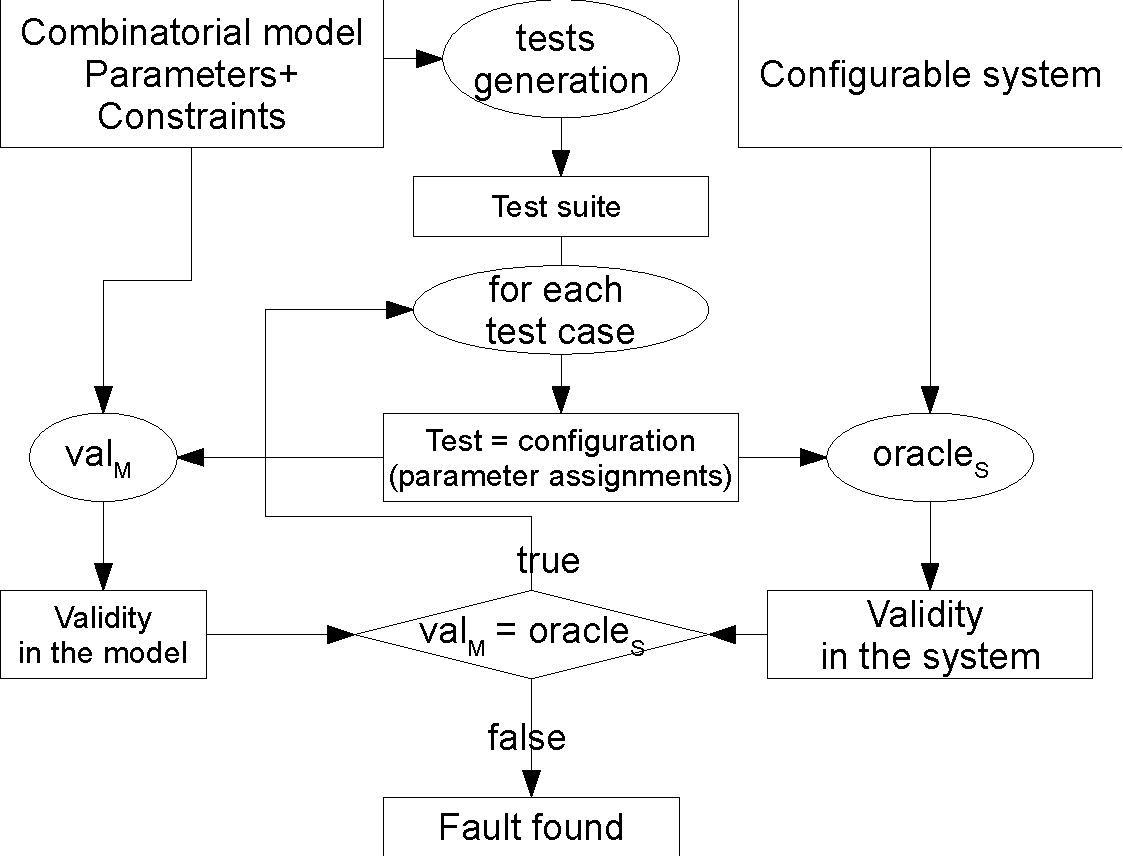
\includegraphics[width=.95\columnwidth]{images/spec_vs_impl}
		\end{center}
		\caption{Validating constraints by CIT}\label{fig:process}
	\end{figure}
	
	\subsection{Finding Faults by Combinatorial Testing}
	
	\bb In order to find possible faults as defined in Definition \ref{def:validation_correctness}, the exhaustive exploration of all the configurations of a large software system is usually impractical. In many cases, the evaluation of $oracle_I$ is time consuming and error prone, so the number of tests one can check on the implementation can be very limited. Instead, we can apply combinatorial testing in order to select the parameters values and check that for every generated CIT test $val_{S}(p) = oracle_I(p)$ holds. This approach does not guarantee, of course, finding all possible conformance faults, but we can assume that faults are due to the interaction of parameters and we can leverage the success of CIT in finding faults in real configurable systems \cite{KuhnTSE04,Petke15:practical}.
	
	We have devised a process that is able to find possible conformance faults. It is depicted in Figure \ref{fig:process}
	and consists of the following steps:
	
	\begin{enumerate}
		\item Create a CIT model $S$ that takes constraints into account.
		\item Generate a CIT test suite according to one of the policies (see Section \ref{sec:validation_citpolicies}).
		\item For every test in the test suite, 
		\begin{enumerate}
			\item Compute its validity as specified by the constraints in the CIT model.
			\item Compute $oracle_I$, by executing the software system under each configuration to check if it's acceptable.%using the same configuration in order to check if the configuration is acceptable
			\item Compare the validity, as defined by the model, with the actual result.
			\item If $val_{S}\neq oracle_{I}$ a fault (either in the model or in the system) is found.
		\end{enumerate}
	\end{enumerate}
	
	A discrepancy between the model and the real system means that a configuration is correct according to the model but rejected by the real system (or the other way around) and this means that the constraints in the model do not correctly describe constraints in the system under test.
	\be
	
	\paragraph{Invalid Configuration Testing.}\label{sec:invalidimportance}
	
	\bb In classical combinatorial interaction testing, only valid tests are generated, since the focus is on assessing if the system under test produces valid outputs. 
	%testing the software implementation. 
	However, we believe that invalid tests are also useful.  In particular,  they address the following issues.
	
	The CIT model should minimise the number of constraints and the invalid configuration set:  invalid configurations, according to the model, should only be those that are actually invalid in the real system. This kind of test aims at discovering faults of over-constraining the model. This problem is a variant of the bigger problem of over-specification. Moreover, critical systems should be tested if they safely fail when the configuration is incorrect. This means that the system should check that the parameters are not acceptable (i.e. it must \emph{fail}) and it should fail in a safe way, avoiding crashes and unrecoverable errors (it must fail \emph{safely}). Furthermore, creation of a CIT model for a large real-world software system is usually a tedious, error-prone task. Therefore, invalid configurations generated by the model at hand can help reveal constraints within the system under test and help refine the CIT model. In line with the scientific epistemology, our research focuses on generating not only tests (i.e., valid configurations) that confirm our theory (i.e., the model), but also tests that can \emph{refute} or  \emph{falsify} it. 
	Since the number of invalid configurations might be huge, such configurations must be chosen in accordance with some criteria. We choose to use the same t-way interaction paradigm as in standard CIT.
	\be
	
	\subsection{Combinatorial Testing Policies}
	\label{sec:validation_citpolicies}
	
	\bb We propose to use search-based combinatorial interaction testing techniques to verify the validity of CIT models. In particular, given a CIT model, we modify it according to one of the policies introduced in this section. Next, we use CASA to generate the test suite satisfying the modified CIT model. 
	We use the term ``valid test" to denote the generated configuration that satisfies all the constraints of the original CIT model. Conversely, the term ``invalid test" is used for a configuration that does not satisfy at least one of the constraints of the original CIT model. Words ``test" and ``configuration" are used interchangeably, though we note in real-world systems one configuration may lead to multiple tests.
	\be
	
	\subsubsection{\ic: Unconstrained CIT.}
	\bb
	In unconstrained CIT, constraints are ignored during CIT test generation.
	They are used only to check the validity of the configuration
	selected during generation. The main advantage is that test generation
	is simplified and efficient methods that work without constraints
	can be used. Moreover, in principle, both valid and invalid configurations
	can be generated - there is no control over
	model validity. It may happen that the test generation algorithm generates
	only valid combinations (i.e., $val_{S}(t)$ for every $t$ in the test
	suite). This may reduce the effectiveness of the test suite: if only valid tests are generated, one can miss faults only discoverable by invalid tests, as explained in Section \ref{sec:invalidimportance}. On the other hand, only invalid tests can be equally useless.
	
	\begin{example}
		In the washing machine example shown in Fig.~\ref{fig:washerexample}, 
		\ic policy will produce a pairwise test suite with at least 9 test cases, including an invalid test case
		where \texttt{HalfLoad} is set to true in combination with \texttt{Spin} equal to 1800.
		%, and tests where \texttt{Rinse} is Delicate, \texttt{HalfLoad} is false, and \texttt{Spin} is greater than 800.
	\end{example}
	\paragraph*{Test generation.}
	\ic can be applied by simply removing the constraints $c_i$ from the original CIT model. The validity of each test can be later computed by checking if the generated configuration satisfies all the $c_i$. There are several CIT tools that do not handle constraints (for example, those that use algebraic methods for CIT test suite generation), hence can be used with this policy.
	
	%\vspace{-0.5em}
	
	
	\subsubsection{\ccit: Constrained CIT.}
	
	In this classical approach, constraints are taken into account and only valid
	combinations among parameters are chosen. Among these parameters
	a certain level of desired strength is required. The rationale behind
	this policy is that one wants to test only valid combinations. If
	a certain interaction among parameters is not possible, then it is
	not considered even if it would be necessary in order to achieve the
	desired level of coverage. The main advantage is that no error should
	be generated by the system. However, this technique can only check
	one side of equation given in Def.~\ref{def:correctness}, namely
	that $val_{S}(p)\rightarrow$$oracle_{I}(p)$, since $val_{S}$ is always
	true. If the specification is too restrictive, %with respect to  the real system, 
	no existing fault will be guaranteed to be found, if it refers to configurations that are 
	invalid. %{*}{*}{*}{*}
	%\vspace{-0.5em}
	\begin{example}
		In the washing machine example shown in Fig.~\ref{fig:washerexample}, the \ccit policy produces 7 tests for pairwise, all of which satisfy the constraints. Some pairs are not covered: for instance \texttt{HalfLoad}=true and \texttt{Spin}=1800 will not be covered.
	\end{example}
	
	\paragraph*{Test generation.} \ccit is the classical constrained combinatorial testing (CCIT), and CASA can correctly deal with the constraints and generate only valid configurations. However, CASA requires the constraints in Conjunctive Normal Form (CNF), so \citlab must convert the constraints from general form to CNF.
	
	\subsubsection{\cv: Constraints Violating CIT.}
	In case one wants to test the interactions of parameters that produce errors, 
	only tests violating the constraints should be produced. This approach is complementary with respect to the \ccit in which only valid configurations are produced. In \cv, we ask that the maximum possible CIT coverage for a given strength is achieved considering only tuples of parameter values that make at least one constraint false (i.e. each test violates the conjunction $c_{1}\wedge \dots\wedge c_{n}$ ). 
	\begin{example}
		In the example presented in Fig.~\ref{fig:washerexample}, the CV policy produces 6 test cases, all of which violate some constraint of the model. For instance, a test has \texttt{Rinse}=Delicate, \texttt{Spin} =800, and \texttt{HalfLoad}=false.
	\end{example}
	\paragraph*{Test generation.} \cv can be applied by modifying the model by replacing all the constraints with $\neg(c_{1}\wedge \dots\wedge c_{n})$ and then classical \ccit is applied.
	
	\subsubsection{\cucv: Combinatorial Union.}
	One limitation of the \ccit technique is that with an over-constrained model, certain faults may not be discovered. On the other hand, by generating test cases violating constraints only, as in \cv, certain parameter interactions may not be covered by the generated test suite. In order to overcome these limitations we propose the combination of \ccit and \cv. %(see Sections \ref{sub:unconstrainedCIT} and \ref{sub:classicalCIT}).
	
	\paragraph*{Test generation.}
	\cucv is achieved by generating tests using policy \ccit and policy \cv and then by merging the two test suites. Since every test is either valid (in \ccit) or invalid (in \cv), merging the test suites consists of simply making the union of the two test suites.
	
	\subsubsection{\ValC: CIT of Constraint Validity.}
	\cucv may produce rather big test suites, since it covers all the desired parameter interactions that produce valid configurations \emph{and} all those that produce invalid ones according to the given CIT model. On the other hand, \ic may be too weak since there is no control over the final constraint validity and therefore there is no guarantee that the parameter values will influence the final validity of the configuration. On one extreme, \ic might produce a test suite without any test violating the constraints. 
	We propose the \ValC policy that tries to balance the validity of the tests without requiring the union of valid and invalid tests. \ValC requires the interaction of each parameter with the validity of the whole CIT model. That is, both tests that satisfy all the constraints will be generated as well as those that don't satisfy any of the constraints in the given CIT model. 
	Formally, \ValC requires that the validity of each configuration $\bar{p}$ (i.e., $val_{S}(\bar{p})$) is covered in the same desired interaction strength (see Definition \ref{def:citstrength}) among all the parameters. %\red{to explain??}. 
	
	\begin{example}
		For the WashingMachine, \cucv generates 13 test cases (6+7). \ValC requires only 11 test cases.
	\end{example}
	\paragraph*{Test generation.}
	\ValC requires to modify the original CIT model by introducing a new Boolean variable \textsf{validity} and replacing all the constraints with one constraint equal to \textsf{validity} $\leftrightarrow (c_{1}\wedge \dots\wedge c_{n})$
	
	
	\subsubsection{\CCi: CIT of the Constraints.}
	Every constraint may represent a condition over the system state. For instance, the constraint
	\lstinline[language=comb]|HalfLoad => Spin < maxSpinHL|
	identifies the critical states in which the designer wants a lower spin speed. One might consider each constraint as a property of the system and be interested in covering how these conditions interact with each other and with the other parameters. The goal is to make the constraints interact with the other system parameters.
	\paragraph*{Test generation.}
	\CCi requires the introduction of a new Boolean variable $\mathsf{validity}_i$ for every constraint, and replacing every constraint $c_i$ with $\mathsf{validity}_i \Leftrightarrow c_{i}$.
	\be
	
	\subsection{Experiments}
	\label{sec:validation_experiments}
	
	\bb In order to test our proposed approach we conducted the following experiments.
	We used 4 case studies to evaluate our proposed approach:
	
	\begin{asparaenum}
		
		\item \textbf{Banking1} represents the testing problem for a configurable Banking application presented in \cite{segall_using_2011}. 
		
		\item \textbf{libssh} is a multi-platform library implementing SSHv1 and SSHv2 written in C\footnote{\url{https://www.libssh.org/}}. The library consists of around 100 KLOC and can be configured by several options and several modules (like an SFTP server and so on) can be activated during compile time. We have analysed the \texttt{cmake} files and identified 16 parameters and the relations among them. We have built a feature model for it in \cite{icst2016} and we have derived from that a \citlab model.
		%
		\item \textbf{\TLSChecker} is a small C program, written by us, that performs a Heartbeat test on a given TLS server. 
		The Heartbeat Extension is a standard procedure (RFC 6520) that tests secure communication links by allowing a computer at one end of a connection to send a ``Heartbeat Request" message. Such a message consists of a payload, typically a text string, along with the payload's length as a 16-bit integer. The receiving computer then must send exactly the same payload back to the sender. \TLSChecker reads the data to be used in the Heartbeat from a configuration file with the following schema:
		
		\begin{center}
			\begin{minipage}{.9\linewidth}%
				\begin{lstlisting}[frame=single,basicstyle={\scriptsize\ttfamily}]
				TLSserver: <IP>
				TLS1_REQUEST Length: <n1> PayloadData: <data1>
				TLS1_RESPONSE Length: <n2> PayloadData: <data2>
				\end{lstlisting}
			\end{minipage}
		\end{center}
		
		
		Configuration messages with \texttt{n1} equal to \texttt{n2} and  \texttt{data1} equal to  \texttt{data2} represent a successful  Heartbeat test (when the TLS-server has correctly responded to the request). \TLSChecker can be considered as an example of a \emph{runtime} configurable system, since thanks to the parameters one can perform different types of tests (with different lengths and payloads). We have written an abstract version of \TLSChecker in the combinatorial model shown in Fig. \ref{fig:TLSChecker}: we ignore the actual content of the PayloadData and we model only the lengths: \textsf{Length} represents the declared lengths and \textsf{PayloadData\_length} is the actual length of the PayloadData. The constraints represent successful exchanges of messages in the Heartbeat test. The oracle is true if the Heartbeat test has been successfully performed with the specified parameters.
		
		\begin{figure}[h]
			\begin{lstlisting}[language=comb,basicstyle=\sffamily\footnotesize]
			Model Heartbeat
			Parameters:
			Range REQ_Length [ 0 .. 65535 ] step 4369;
			Range REQ_PayloadData_length [ 0 .. 65535 ] step 4369;
			Range RES_Length [ 0 .. 65535 ] step 4369;
			Range REQ_PayloadData_length [ 0 .. 65535 ] step 4369;
			end
			Constraints:
			// the declared length in the REQUEST is correct
			# REQ_Length==REQ_PayloadData_length #
			// the declared length in the RESPONSE is correct
			# RES_Length==RES_PayloadData_length #
			// the RESPONSE has the same length as the REQUEST
			# REQ_Length==RES_Length #	
			end
			\end{lstlisting}
			\caption{\TLSChecker CIT model}
			\label{fig:TLSChecker}
		\end{figure}
		
		
		\item \textbf{Django}  is a free and open source web application framework, written in Python, consisting of over 17k lines of code, that supports the creation of complex, database-driven websites, emphasizing reusability of components\footnote{\url{https://www.djangoproject.com/}}. Each Django project can have a configuration file, which is loaded every time the web server that executes the project (e.g. Apache) is started. Therefore, the configuration parameters are loaded at \emph{launch time}.
		In the model we made, among all the possible configuration parameters, we selected and considered one Enumerative and 23 Boolean parameters. We elicited the constraints from the documentation, including several forum articles and from the code when necessary. We have also implemented the oracle, which is completely automated and returns true if and only if the HTTP response code of the project homepage is 200 (HTTP OK).
	\end{asparaenum}
	\be
	
	\begin{table*}[h]
		\caption{Benchmark data. {\footnotesize $vr$ is the validity ratio, defined as the percentage of configurations that are valid.}}\label{tab:validation_benchmarks}
		\centering
		\begin{tabular}{lrrrrrrrrr}
			\toprule
			name & \#var & \multicolumn{1}{c}{\#constraints} &\multicolumn{1}{c}{\#configurations} & \multicolumn{1}{c}{$vr$} & \multicolumn{1}{c}{\#pairs}\\ 
			\midrule
			Banking1 & 5 & 112 & 324 & 65.43\% &  102  \\ 
			Libssh &  16 & 2 &  65536  & 50\% & 480 \\ 
			\TLSChecker & 4 & 3 & 65536 & 0.02\% & 1536 \\ 
			Django & 24 & 3 &  33554432 & 18.75\% & 1196\\
			\bottomrule
		\end{tabular}
		%}
	\end{table*}
	
	
	\bb Table \ref{tab:benchmarks} presents various benchmark data: number of variables and constraints, 
	size of the state space (the total number of possible configurations), the percentage of configurations that are valid  (i.e. the ratio $vr$), the number of pairs that represent the pairwise testing requirements (ignoring constraints). Note that a low ratio indicates that there are only few valid configurations (see, for example, the \TLSChecker benchmark). We collected models of real-world systems from different domains, with a good level of diversity (in terms of size, constraints, etc.) in order to increase the validity of our findings.
	
	Experiments were executed on a Linux PC with two Intel(R) i7-3930K CPU  (3.2 GHz) and 16 GB of RAM. All reported results are the average of 10 runs with a timeout for a single model of 3600 secs. Test suites were produced using the CASA CIT test suite generation tool according to the pairwise testing criterion.
	\be
	
	\subsubsection{Test generation and coverage}
	
	\bb In our first experiment, we are interested in comparing the policies in terms of test \emph{effort} measured by the number of tests and by the test suite generation time.
	Table \ref{tab:gendata} presents the following data:
	\begin{itemize}
		\item The \emph{time} required to generate the tests and to evaluate their validity (it does not include the evaluation of the $oracle_{I}$) in seconds.
		\item The \emph{size} in terms of the number of tests and how many of those are valid (\#Val), i.e.   $val_{S}$  returns true. %(\red{would in percentage be useful?})
		\item The percentage of parameter interactions (pairs) that are covered. In the count of the pairs to be covered, we ignore constraints as in Table \ref{tab:benchmarks}.
	\end{itemize}
	\be
	
	\begin{table*}[t]
		\caption{Valid pairwise parameter interactions covered by six test generation policies. (Shaded cells are covered in the prose.) Out of memory errors are due to constraint conversion into the CNF format required by CASA. In particular, as known in the literature, the size in CNF of the negation of a constraint can grow exponentially.}\label{tab:gendata} %Interesting cases covered in the prose are shaded.
		\centering
		\resizebox{\columnwidth}{!}{%
			\begin{tabular}{l|cccc|cccc|cccc|cccc}
				\toprule
				&   \multicolumn{4}{c}{Banking1} & \multicolumn{4}{c}{Django}  &   \multicolumn{4}{c}{libssh} &\multicolumn{4}{c}{\TLSChecker}\\
				Pol.  & time & size  & \#Val & Cov. & time& size  & \#Val & Cov. & time& size  & \#Val & Cov. & time& size  & \#Val & Cov.  \\ \midrule
				\ic & 0.22 & 12 & 11 & 100\% & 0.65 & 10 & 2 & 100\%& 0.25 & 8 & 4 & 100\% & 447 & 267 & \cellcolor{light-gray}0 & 100\%\\
				\ccit & 0.26 & 13 & 13 & \cellcolor{light-gray}100\%&  1.24 & 10 & 10 & 91.8\%& 0.28 & 8 & 8 & 99.3\% & 2.74 & 141 & 141 & 6.2\%\\
				\cv &\multicolumn{4}{c}{Out of memory} &  0.32 & 11 & 0 & \cellcolor{light-gray}100\%& 0.25 & 8 & 0 & 99.3\% &\multicolumn{4}{c}{Out of memory} \\
				\cucv &\multicolumn{4}{c}{Out of memory} &  1.58 & 21 & 10 & 100\% & 0.52 & 16 & 8 & 100\% &  \multicolumn{4}{c}{Out of memory}\\
				\ValC &\multicolumn{4}{c}{Out of memory} &   0.31 & 11 & 4 & 100\%& 0.29 & 8 & 5 & 100\% &  \multicolumn{4}{c}{Out of memory} \\
				\CCi & 6.22 & 12 & 9 & 100\% & 0.58 & 13 & 3 & 100\%&  0.30 & 8 & 2 & 100\% &  460 & 268 & \cellcolor{light-gray}0 & 100\%\\\bottomrule
			\end{tabular}
		}
	\end{table*}
	
	\bb \noindent From Table  \ref{tab:gendata} we can draw the following observations:
	
	\begin{asparaitem}
		
		\item 
		\ic usually produces both valid and invalid tests. However, it may produce all invalid tests (especially if the constraints are strong - see \TLSChecker). Having all invalid tests may reduce test effectiveness.
		
		\item 
		\ccit usually does not cover all the parameter interactions, since some of them are infeasible because they violate constraints in the original model. On the other hand, \ccit generally produces smaller test suites (as in the case of \TLSChecker). However, in some cases, \ccit is able to cover all the required tuples at the expense of larger test suites (as in the case of Banking1). 
		
		\item 
		\cv generally does not cover all the parameter interactions, since it produces only invalid configurations. However, in one case (Django) \cv covered all the interactions. This means that 100\% coverage of the tuples in some cases can be obtained with no valid configuration generated and this may reduce the effectiveness of testing. %Therefore, interaction coverage may be not a good indicator of the coverage of the model validity by itself.
		Sometimes \cv is too expensive to perform.
		
		\item
		\cucv guarantees to cover all the interactions and it produces both valid and invalid configurations. However, it produces the bigger test suites and it may fail because it relies on \cv.
		
		\item 
		\ValC covers all the interactions with both valid and invalid configurations. It produces test suites smaller than \cucv and it is generally faster, but as \cucv may not terminate.
		
		\item
		\CCi covers all the interactions, it generally produces both valid and invalid test. However, it may produce all invalid tests (see \TLSChecker), and it produces a test suite comparable in size with \ic. However, it guarantees an interaction among the constraint validity. It terminates, but it can be slightly more expensive than \ic and \ccit. If the strength of combinatorial testing is greater or equal to the number of constraints, it guarantees also that valid and invalid configurations are generated.
	\end{asparaitem}
	\be
	
	\subsubsection{Fault detection capability}
	
	\bb We are interested in evaluating the fault detection capability of the tests generated by the policies presented above. 
	We have applied mutation analysis \cite{surveyMutationTesting} which consists of introducing artificial faults and checking if the proposed technique is able to find them. In our case, we have introduced the faults by hand and then we have applied our technique described in Section \ref{sec:process} in order to check if the fault is detected (or \emph{killed}). 
	Tables in Fig. \ref{tab:faultdetection} present a brief description of each introduced fault and if each policy was able to kill it.
	
	In principle, our technique is able to find conformance faults both in the model and in the implementation. Indeed, when a fault is found, it is the designer's responsibility to decide what is the source of the fault. For libssh we have modified both the model and the code (the \texttt{cmake} script) (faults L$x$). For the  \TLSChecker we have modified the model and the source code (faults H$x$). Table in Fig. \ref{fig:seededfaults} presents the details of each injected fault, including if it refers to the specification (S) or to the implementation (I).
	\be
	
	\begin{figure}[h]%
		\centering
		\begin{subfigure}[b]{0.32\textwidth}
			\resizebox{\columnwidth}{!}{\begin{tabular}{ccll}
				\parbox[t]{3mm}{\multirow{5}{*}{\rotatebox[origin=c]{90}{libssh}}}
				& L1&forgot all the constraints	 &S\\
				& L2&remove a constraint	&S\\
				& L3&add a constraint	&S\\
				& L5	& remove a dependency&I\\
				& L6	& add a dependency&I\\\\
				\parbox[t]{3mm}{\multirow{6}{*}{\rotatebox[origin=c]{90}{HeartBeatChecker}}}
				& H1  & remove one constraint&S\\
				& H2	&== to $<=$&S\\
				& H4	&\&\& to $||$	&I\\
				& H5	&== to != (all)	&I\\
				& H6	&== to != (one) &I\\
				& H7	&HeartBleed	&I \\\\
		\end{tabular}}
		\caption{Seeded Faults (S: in Spec, I: in implementation)}\label{fig:seededfaults}
		\end{subfigure}
		\begin{subfigure}[b]{0.61\textwidth}
			\centering
			\resizebox{\columnwidth}{!}{\begin{tabular}{lccccccccccccccr}
				\\
				&&\multicolumn{13}{c}{Is the fault detected?} & mut.\\
				Policy & &L1 &L2	&L3	&L4	& L5&	L6	&	H1	&H2&	H3	& H4	&	H5	& H6 & H7 & score\\\midrule
				\ic	&&	\checkmark & 	 \checkmark & 		&	 \checkmark & 	 \checkmark & 		&	 \checkmark & 	 \checkmark & 	 \checkmark & 	 \checkmark & 	 \checkmark & 	 \checkmark & 		& 10/13\\
				\ccit	&&	 \checkmark & 	 \checkmark & 		&	&	&	 \checkmark & 	 \checkmark & 	 \checkmark & 	 \checkmark & 		&	 \checkmark & 		&	& 7/13\\
				\cv	&&	 \checkmark & 		&	 \checkmark & 	 \checkmark & 	 \checkmark & 		&- & - & - & - & - & - & - & 4/13 \\
				\cucv	&&	 \checkmark & 	 \checkmark & 	 \checkmark & 	 \checkmark & 	 \checkmark & 	 \checkmark & - & - & - & - & - & - & - & 		6/13\\
				\ValC	&&	 \checkmark & 	 \checkmark & 		&	 \checkmark & 	 \checkmark & 		&	 - & - & - & - & - & - & - & 	4/13\\
				\CCi	&&	 \checkmark &  	 \checkmark & 	 \checkmark & 	 \checkmark & 	 \checkmark & 		&	 \checkmark & 	 \checkmark & 	 \checkmark & 	 \checkmark & 	 \checkmark & 	 \checkmark & 		 \checkmark & 12/13\\\\\\\\
			\end{tabular}}%
			\caption{Fault detection capability of the policies (- means that the test suite was not generated.)}\label{fig:faultdetected}
		\end{subfigure}			
		\caption{Fault detection capability}
		\label{tab:faultdetection}
	\end{figure}
	
	\bb Table in Fig. \ref{fig:faultdetected} reports which faults were killed by each policy.
	We can observe that the  unconstrained CIT (\ic) policy performs better than some policies that consider constraints (\ccit and \cv) even if normally their test suites have the same dimensions. However, in some cases (L6) \ccit detected a fault where \ic failed.  For \cv, \cucv, and \ValC we can analyze only the results for libssh, since they did not complete the test generation for \TLSChecker. However, even if we restrict to libssh, \cucv has a very good fault detection capability (but it produces the biggest test suite) while \ValC and \cv scored as well as \ic, although they are more expensive, so according to our studies there is no particular reason to justify the use of \ValC and \cv alone. However,  in one case (L3) \cv detected a fault that \ic did not.
	
	Overall \CCi was the best in terms of fault detection, even with test suites as big as those for \ic. However, it missed one of the injected faults (L6).  
	\CCi was the only one to find the fault H7 (\emph{HeartBleed}).  The HeartBleed fault simulates the famous Heartbleed security bug of the OpenSSH implementation of the TLS protocol. It results from improper input validation (due to a missing bounds check) in the implementation of the TLS Heartbeat extension. In detail, the implementation built the payload length of message to be returned based on the length field in the requesting message, without regard to the actual size of that message's payload. In our implementation, the faulty \TLSChecker missed to check that \lstinline[language=comb]$REQ_Length==RES_Length$. This proves that testing how parameters can interact with single constraints increases the fault detection capability of combinatorial testing. Our new policies may thus prove useful in detecting faults missed by standard approaches due to the so-called \emph{masking effects} \cite{YilmazDCP14}. \be


\section{Combinatorial Interaction Testing for Automated Constraint Repair}\label{sec:constr}

%%% RATIONALE

Most software systems can be configured in order to improve their capability to address users' needs. Configuration of such systems is generally performed by setting system parameters. These options, or \emph{features}, can be created during design time. For instance, in the case of a \emph{software product line}, the designer identifies the features unique to individual products and features common to all products in its category.
%the designer models the features of the products that are in common and the features that can vary among the several products belonging to the same family. 

Such options can also be decided during compilation time, in order to improve some characteristics of the compiled code (scalability, efficiency, etc.). For example, in case of preprocessor directives, the programmer can decide which libraries to use, what code to execute and what to ignore etc. Software configurations can also be modified during operation time, when the system is already running and the user wants to switch on/off a particular feature or functionality. In this case, for example, the parameters can be saved in a configuration file and modified if necessary. Such a configuration file can also be used to decide which features to load at startup.
%Justyna: the model is unreadable, hence I removed the figure
%An example is depicted in Figure \ref{fig:problemsolution}. The picture presents a washing machine and model of its configurations. 
The \emph{problem space} described by the model of its configurations shows its supported features and
their dependencies, while the \emph{solution space} is the technical realisation of the system \cite{NadiBKC14}, i.e., its implementation.


Large configurable systems and software product lines can have hundreds of features. It is infeasible in practice to test all the possible configurations.  Consider, for example, a system with only 20 Boolean parameters. One would have to check over one million configurations in order to test them all. 

\noindent Furthermore, the time cost of running one test could range from fraction of a second to hours if not days. In order to address this combinatorial explosion problem, combinatorial interaction testing (CIT) has been proposed for testing configurable systems \cite{CohenISSTA07}. It is a very popular black-box testing technique that tests all interactions between any set of $t$ parameters.  There have been several studies showing the successful efficacy and efficiency of the approach \cite{KuhnTSE04,Kuhn06:pseudo,Petke15:practical,Petke2013a}.  

%\red{CIT has been proposed for testing configurable systems, especially in the presence of constraints \cite{CohenISSTA07}}.

Moreover, certain tests could prove to be infeasible to run, because the system being modelled can prohibit certain interactions between parameters. 
%Besides identifying the parameters and their possible values, there can be constraints among these parameters. 
Designers, developers, and testers can greatly benefit from modelling parameters and constraints among them by significantly reducing modelling and testing effort \cite{Petke15:practical} as well as identifying corner cases of the system under test. 
Constraints play a very important role, since they identify parameter interactions that need not be tested, hence they can significantly reduce the testing effort.
Certain constraints are defined to prohibit generation of test configurations under which the system simply should not be able to run.  
Other constraints can prohibit system configurations that are valid, but need not be tested for other reasons. For example, there's no point in testing the \emph{find} program on an empty file by supplying all possible strings. %\red{elaborate one this - the importance about constraints} 

Constructing a CIT model of a large software system is a hard, usually manual task.  Therefore, discovering constraints among parameters is highly error prone. One might run into the problem of not only producing an incomplete CIT model, but also one that is over-constrained. Even if the CIT model only allows for valid configurations to be generated, it might miss important system faults if one of the constraints is over-restrictive. Moreover, even if the system is not \emph{supposed} to run under certain configurations, if there's a fault, a test suite generated from a CIT model that correctly mimics only desired system behaviour will not find that error. In such situations tests that exercise those corner cases are desirable. 

%\red{Reviewer: an important obvious use case for our method is software evolution. The initial model can conform with the system, but when the system or its configuration space undergo changes, the model becomes non-conforming and needs to be repaired. There is a clear motivation for automated repair in this use case.}

Software evolution is a typical scenario in which automated repair of the model of system's configurations may be useful. The initial model can conform with the system, but when the system or its configuration space undergo changes, the model becomes non-conforming and needs to be repaired.

The problem of finding and fixing conformance faults between a given software system and its combinatorial model is a challenging task. Due to the size and complexity of current software systems, the interactions between different software parameters are hard to find. Combinatorial models are frequently derived manually, by expert software engineers. The Software-artefact Infrastructure Repository\footnote{\url{http://sir.unl.edu/portal/index.php}}, for instance, contains models of dozens of software systems, which were derived by hand. 

Several methods have been introduced to automate the process of inferring constraints. However, they do not guarantee that the derived model will be correct~\cite{Temple16:using}. Therefore,

\vspace{0.2em}
\noindent \textit{\textbf{we introduce a novel automated approach for finding and fixing conformance faults between the given software system and its combinatorial model}}. 
\vspace{0.2em}

We use combinatorial interaction testing policies introduced in our previous work~\cite{Gargantini16:validation} to find such faults and fix them by repairing constraints in the original CIT model.

We conduct several experiments aiming to answer the following research questions:

\vspace{0.2em}
[\textbf{RQ1:}] \emph{How effective is our automated constraint repair approach at fixing faults in an existing CIT model?}\\
In particular, we apply our approach to mutated CIT models and show that our approach can automatically fix on average 37\% of conformance faults.

\vspace{0.2em}
[\textbf{RQ2:}] \emph{How effective is our approach in inferring parameter constraints in real-world software?}\\
We present a case study that shows that our approach can be used to derive constraints for an unconstrained CIT model of a large real-world software system.

\vspace{0.2em}
[\textbf{RQ3:}] \emph{How efficient is our constraint repair approach?}\\
In order to evaluate the efficiency of our approach, we measure the time taken to repair constraints in CIT models as well as the number of tests needed for the repair. On the five systems evaluated, the mutated models were repaired within seconds.
\vspace{0.2em}

This section reports the content of the paper \cite{gargantini_combinatorial_2017}, and it is structured as follows: Section \ref{sec:citmodels} gives a brief overview of combinatorial interaction testing activities with the \citlab tool; Section \ref{sec:citpolicies} briefly describes CIT policies used in our approach; Section \ref{sec:defs} presents definitions and notation used throughout our paper; Section \ref{sec:repair} presents our approach to fixing conformance faults between a software system and its combinatorial model; Section \ref{sec:experiments} contains experimental results and answers to research questions posed; and Section \ref{sec:relatedwork} presents related work. Conclusions and future work are discussed jointly at the end of the chapter, in Section \ref{sec:conclusions}.

\subsection{Combinatorial Models and Testing of Configurable Systems}
\label{sec:citmodels}

\bb Combinatorial Interaction Testing (CIT), often called combinatorial
testing or combinatorial testing design, aims to test 
configurable software systems under the various combinations of its parameter values. 
There exist several tools and techniques for CIT. Good surveys of ongoing research in CIT can be found in~\cite{GrindalSTVR05,NieL11},
while an introduction to CIT and its efficacy in practice can be found
in~\cite{kuhncomputer09,Petke15:practical}. \be

\subsubsection{Combinatorial models and \citlab{}\label{sec:citAndCitlab}}

\bb A model for a combinatorial problem
consists of several parameters (at least 2) which can take various domain values. 
In most configurable systems, constraints (or dependencies)
exist between parameters. 

Constraints might be introduced for several
reasons, for example, to model inconsistencies between certain hardware
components, limitations of the possible system configurations, or
simply because of design choices~\cite{CohenISSTA07}. Constraints were first
described as being important to combinatorial testing in~\cite{AETG}
and were introduced in the AETG system. In our approach tests that
do not satisfy the constraints in the CIT model are considered \emph{invalid}.

In this paper we assume that the models are specified using \citlab{}~\cite{citlab12,citlab13ttt}.
This is a framework for combinatorial testing which provides
a rich abstract language with precise formal semantics for specifying
combinatorial problems, an eclipse-based editor with a rich set of
features (syntax highlighting, autocompletion, outline view, and others),
and a Java API library which includes utility methods for generating
all the test requirements for combinatorial coverage of given
strength. \citlab{} does not have its own test generators, but it
relies on other off-the-shelf tools, namely 
ACTS\footnote{\url{http://csrc.nist.gov/groups/SNS/acts/}} and CASA\footnote{\url{http://cse.unl.edu/~citportal/}}.

In \citlab parameters and constraints are given in a unique file
that contains the whole model. To formally describe
a combinatorial problem, the user has to identify at least 2 parameters
and their possible values. 

\begin{defn}[Constrained Model] 
	Let $P=\{p_{1},\dots,p_{m}\}$ be the
	set of parameters. Every parameter $p_{i}$ can take a value from the
	domain $D_{i}=\{v_{1}^{i},\ldots,v_{o_{i}}^{i}\}$. Every parameter
	has a name (it can have also a type with its own name) and every
	enumerative value has an explicit name. We denote with $\mathit{Constr}=\{c_{1},\ldots,c_{n}\}$
	the set of constraints. $P$ and $\mathit{Constr}$ constitute the CIT model.
\end{defn}

\begin{defn}[Strength of a test suite]\label{def:citstrength}
	The objective of a CIT test suite is to cover all parameter interactions between any set of $t$ parameters. $t$ is called the strength of the CIT test suite. For example, a pairwise test suite covers all combinations of values between any 2 parameters.
\end{defn}

\citlab{} adopts the language of propositional logic with equality
and arithmetic to express constraints. To be more precise, it uses
propositional calculus, enriched with the arithmetic over integers
and enumerative symbols. As operators, it admits the use of equality
and inequality for any variable, the usual Boolean operators for Boolean
terms, and the relational and arithmetic operators for numeric terms.

Figure~\ref{fig:washerexample} shows the \citlab{} model
of a simple washing machine consisting of 3 parameters. 
Users can select if the machine has \textsf{HalfLoad}, the desired \textsf{Rinse}, and the speed of \textsf{Spin} cycle.
In the \textsf{Constraints} section there are two constraints: if \textsf{HalfLoad} is set then the speed of spin cycle cannot be \textsf{High}; if rinse is set to \textsf{delicate}, then \textsf{HalfLoad} must be true.\be

\begin{figure}[h]
	\centering 
	\begin{lstlisting}[language=comb]
	Model WashingMachine
	Parameters:
	Boolean HalfLoad;
	Enumerative Rinse { Delicate Drain Wool };
	Enumerative Spin { Low Mid High };
	end
	Constraints:
	# HalfLoad => Spin != Spin.High #
	# Rinse==Rinse.Delicate => HalfLoad #
	end\end{lstlisting}
	\protect\caption{An example CIT model of a washing machine.}\
	\label{fig:washerexample} 
\end{figure}


\subsubsection{Combinatorial Testing Policies}
\label{sec:citpolicies}

\bb
In our previous work \cite{Gargantini16:validation} we proposed to use combinatorial interaction testing techniques to verify the validity of CIT models, which is the approach we use in this work. 

In particular, given a CIT model, we modify it according to one of the policies briefly described below. 
Next, we use one of the standard CIT tools to generate a test suite satisfying the modified CIT model. %In the following subsection we describe the various policies we use to amend the original CIT model.

We use the term ``valid test" to denote the generated configuration that satisfies all the constraints of the original CIT model. Conversely, the term ``invalid test" is used for a configuration that does not satisfy at least one of the constraints of the original CIT model. Words ``test" and ``configuration" are used interchangeably.

In classical combinatorial interaction testing, only valid tests are generated, since the focus is on assessing if the system under test produces valid outputs. 
However, we believe that invalid tests are also useful.  In particular, a combinatorial model can be overconstrained, that is, it might restrict generation of test cases that are valid in the system, yet not be generated due to the constraints in the given model. Furthermore, critical safety systems should be tested if they failed safely in case an invalid configuration is entered. Moreover, creation of a CIT model for a large real-world software system is usually a tedious, error-prone task. Therefore, invalid configurations generated by the model at hand can help reveal constraints within the system under test and help refine the combinatorial model.

Two basic policies can be employed in combinatorial testing: \ic (Unconstrained CIT) consists in generating the tests ignoring the constraints, and \ccit (Constrained CIT) is the classical testing policy that generates only tests satisfying the constraints. Aside from \ic and \ccit, we consider three other policies, introduced in our previous work~\cite{Gargantini16:validation}:

%\vspace{-0.5em}
\subsubsection{Constraints Violating CIT - \cv}
%\vspace{-0.5em}
This approach produces only the tests violating the constraints, i.e. the produced test suite contains every tuple of parameter values that makes at least one constraint false. This approach is complementary with respect to the \ccit in which only valid configurations are produced.

\subsubsection{Combinatorial Union - \cucv}
%\vspace{-0.5em}
\cucv is the union of \ccit and \cv, i.e. it covers all the desired parameter interactions producing valid configurations \emph{and} all those producing invalid ones according to the given CIT model.

\subsubsection{CIT of Constraint Validity - \ValC}
%\vspace{-0.5em}
\ValC requires the interaction of each parameter with the validity of the whole CIT model. That is, both tests that satisfy all the constraints will be generated as well as those that don't satisfy any of the constraints in the given CIT model. \ValC is an approach that tries to balance the validity of the tests without requiring the union of valid and invalid tests.

\be

\subsection{Definitions}
\label{sec:defs}

\bb
We assume that the combinatorial model specifies the parameters and constraints between them for a given software system. 
We are interested in checking whether this system specification 
correctly represents the software implementation. We assume that the parameters and their domains are correctly captured in the specification, while the constraints may contain some faults. 
Software model $M$ belongs to the problem space while implementation of the software system $S$ belongs to the solution space~\cite{NadiBKC14}.
In our repair process, we assume that the model $M$ may contain faults (in the constraints), as opposed to classical software testing, in which the implementation $S$ is to be checked against a model that is considered correct.



Formally, given an assignment $t$ 

that assigns a value to every parameter in $P$ of the model $M$,
we introduce two functions:
\begin{defn}%[Oracle]
	Given a model $M$ for a software system $S$, $val_{M}$ is the function
	that checks if assignment $t$ 
	%$\bar{p}$ 
	satisfies the constraints in $M$, while
	$\mathit{oracle}_{S}(t
	%$\bar{p}$
	)$ checks if $t$ 
	%$\bar{p}$ 
	is a valid configuration according to the system $S$.
	%implementation $I$.
\end{defn}


We assume that the oracle function $\mathit{oracle}_{S}$ exists. For instance, in case of a compile-time configurable system, we can assume that the compiler plays the role of an oracle: if the parameter assignment $t$ allows compilation of the product then we say that $\mathit{oracle}_{S}(t)$ holds. We might enhance the definition of oracle by considering also other factors, for example, if the execution of the test suite completes successfully. However, executing  $\mathit{oracle}_{S}$ might be very time consuming and it might require, in some cases, human intervention.

On the model side, the evaluation of  $val_{M}(t
%\bar{p}
)$ is straightforward, that is, $val_{M}(
%\bar{p}
t)=c_{1[P\leftarrow
	%\bar{p}
	t]}\wedge \ldots\wedge c_{n[P\leftarrow
	%\bar{p}
	t]}$.


\begin{defn}[Conformance fault]
	\label{def:correctness}We say that the constrained CIT model is correct if, for
	every $t$, $val_{M}(t)=\mathit{oracle}_{S}(t)$. We say that the model
	contains a \emph{conformance} fault if there exists a $t$ 
	%$\bar{p}$ 
	such that $val_{M}(
	%\bar{p}
	t)\neq \mathit{oracle}_{S}(
	%\bar{p}
	t)$.
\end{defn}
\be

\begin{figure}[h]
	\begin{center}
		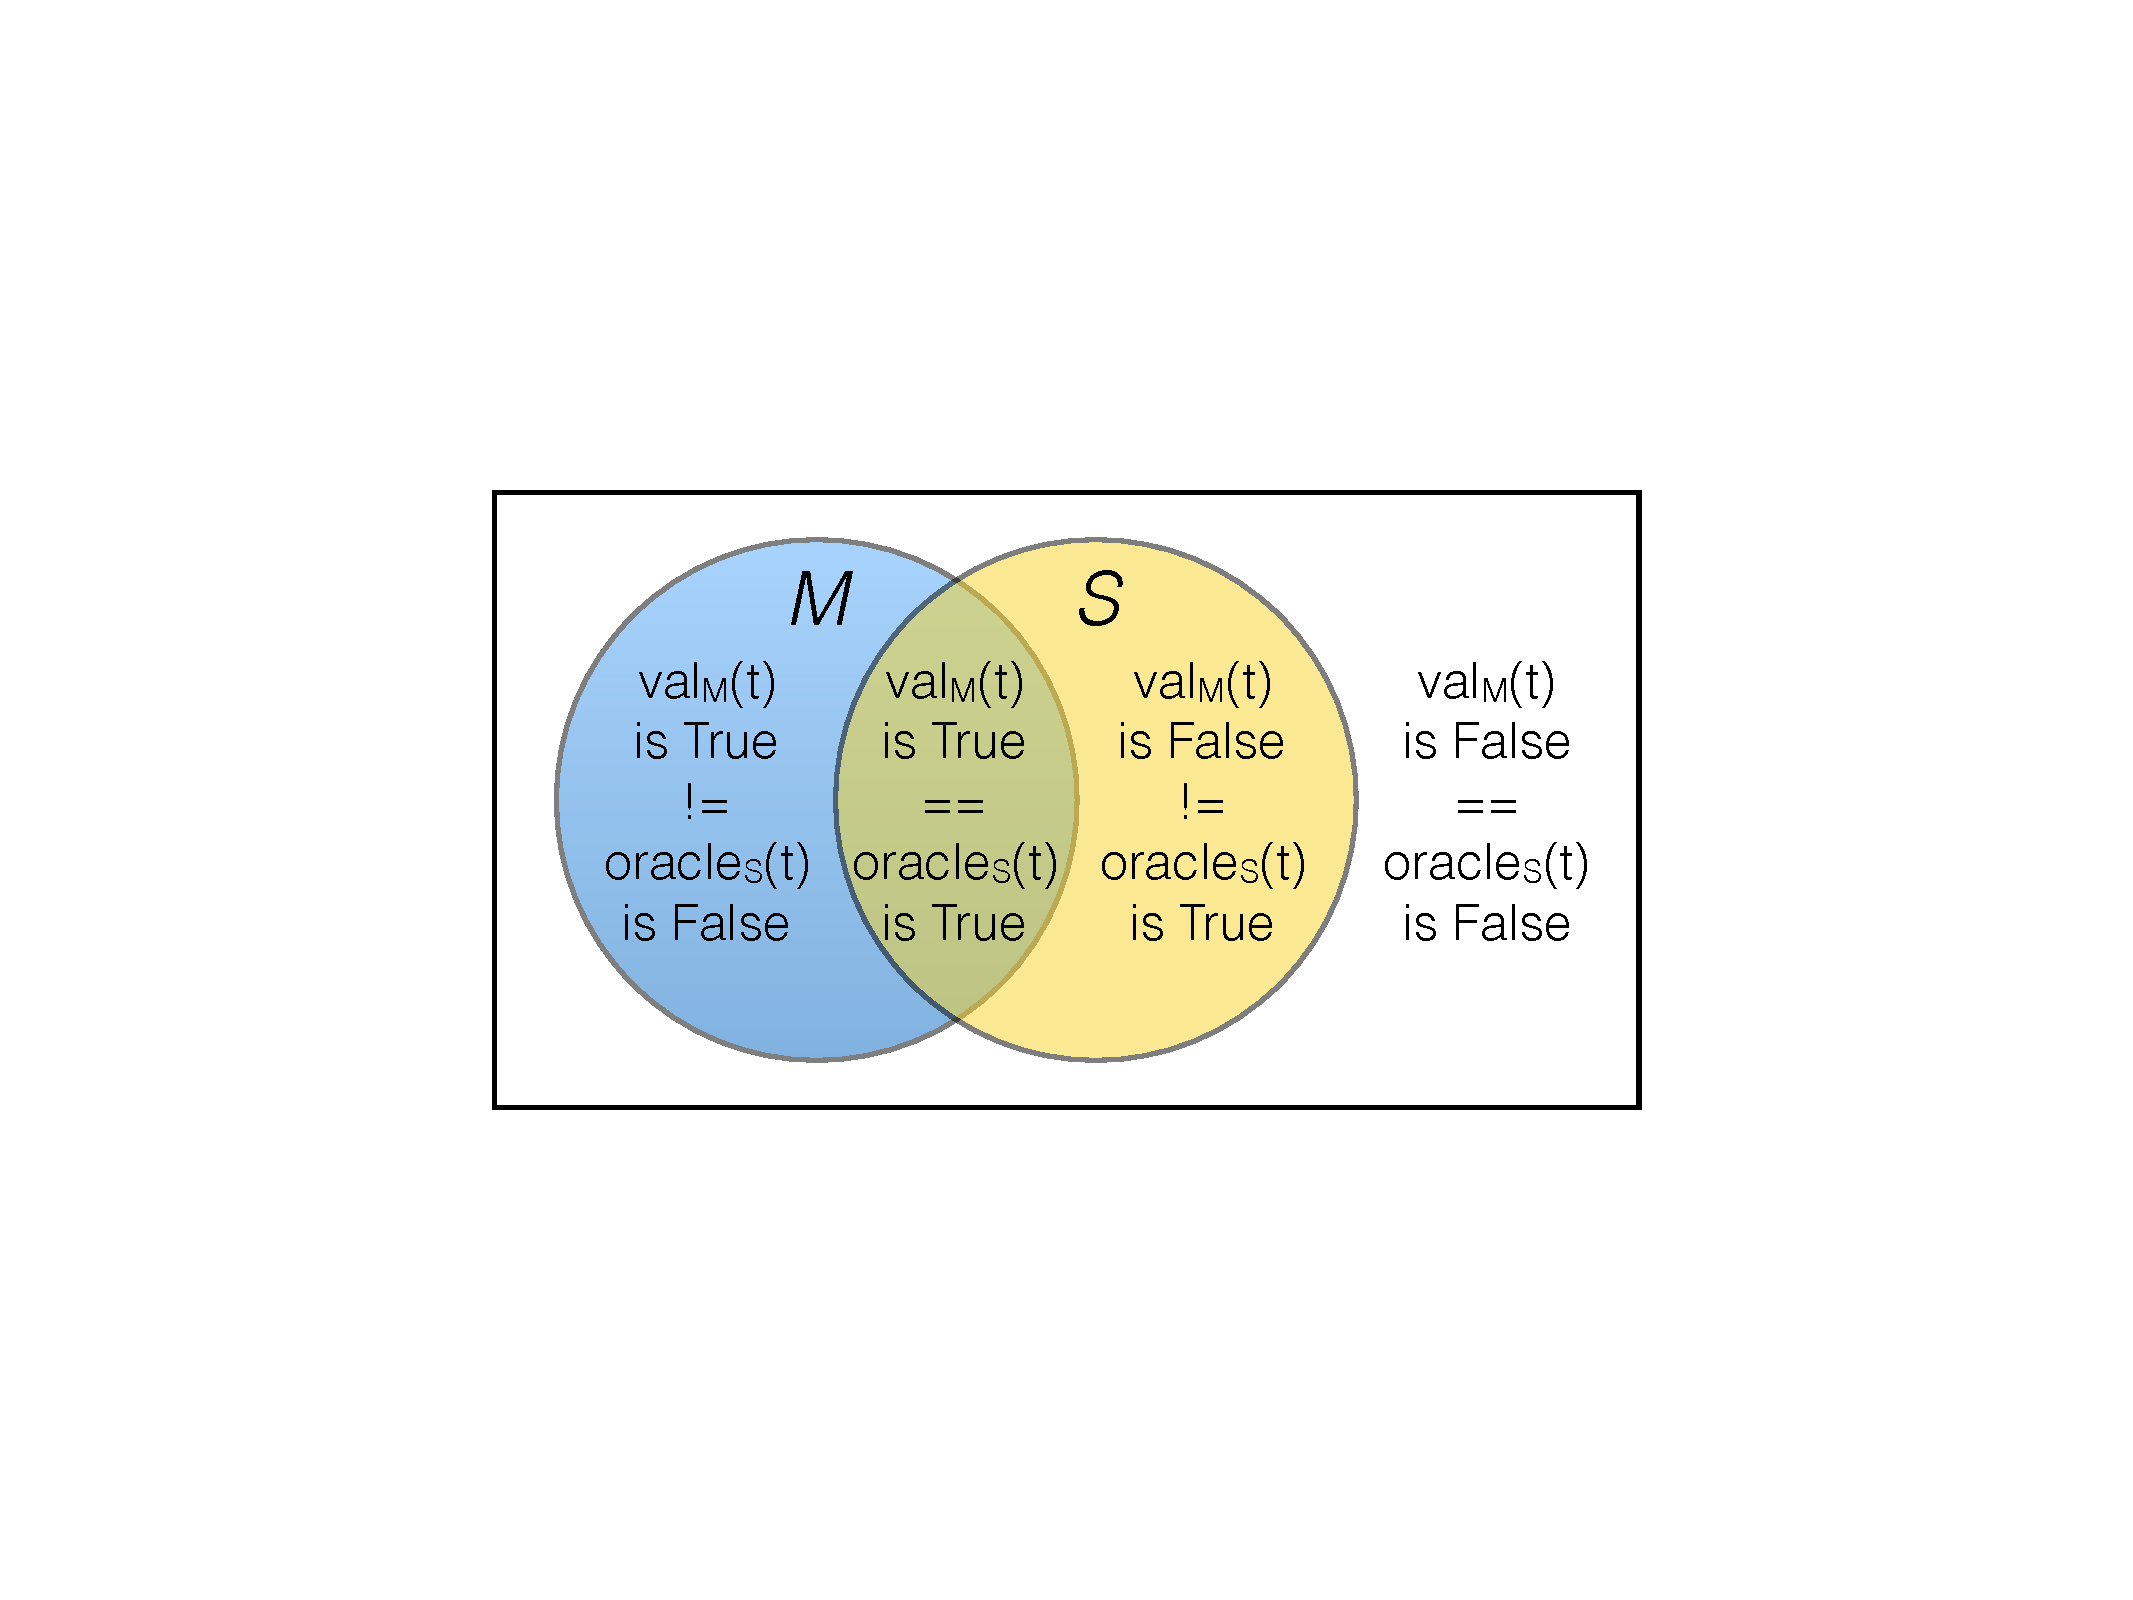
\includegraphics[width=0.6\columnwidth]{images/venndiagram.pdf}
	\end{center}
	\caption{The space of test cases for system $S$ and its model $M$. Failing test cases appear in the regions $M / S$ and $S / M$, i.e., where $val_{M}(t) \neq \mathit{oracle}_{S}(t)$.}
	\label{fig:correctAndFaults}
\end{figure}
%\newpage

\bb 
Figure~\ref{fig:correctAndFaults} shows two different types of failing tests with respect to all possible parameter assignments (ignoring constraints). 
A conformance fault might occur if $val_{M}(t)$ is $\mathit{True}$ and $\mathit{oracle}_{S}(t)$ is $\mathit{False}$ (i.e., $M/S$ in Figure \ref{fig:correctAndFaults}). Another type of conformance fault occurs, when the model does not pass a test case that is allowed by the system, that is, if $\mathit{oracle}_{S}(t)$ is $\mathit{True}$, but $val_{M}(t)$ is $\mathit{False}$ (i.e., $S/M$ in Figure \ref{fig:correctAndFaults}).\be
\begin{example}
	\bb As an example, consider a system $S$ of the washing machine modelled in Figure~\ref{fig:washerexample}, and as model $M$ the same model in Figure~\ref{fig:washerexample} without the first constraint: that conformance fault could be revealed by the following test $t$:\be
	
	\begin{table}[h]
		\centering
		\begin{tabular}{ccc|cc}
			\multicolumn{3}{c|}{Parameter Assignments} & \multicolumn{2}{c}{Function Evaluation} \\ 
			\hline
			Rinse & HalfLoad & Spin & $\mathit{oracle}_{S}$ & $val_M$ \\
			\hline 
			Delicate & True & High & False & True \\ 
		\end{tabular} \label{tab:conformanceFaultExample} \caption{An example test case triggering a conformance fault in the washing machine model.}
		\label{ex:conformancefault}
	\end{table}
\end{example}

\bb
\begin{defn}[Combination]\label{def:cobo}
	Let $P$ be the set of all parameters in a given model. A combination $comb$ is an assignment of values to every parameter in a (non-empty) subset of $P$ . %(the set of all parameters of the model). 
\end{defn}


\begin{defn}[Failure-inducing]
	\label{def:failureinducing}
	A combination $comb$ is failure-inducing if for every test $t$ containing $comb$ (i.e., $comb \subseteq t$), $val_{M}(t) \neq \mathit{oracle}_{S}(t)$.
\end{defn}
\be

\begin{example}\label{ex:ficombo_constraining}
	\bb Given the System $S$ of the washing machine modelled in Figure~\ref{fig:washerexample}, and its Model $M$ presented in Figure~\ref{fig:washerexample} without the first constraint: a failure-inducing combination in this case would be HalfLoad and Spin=Spin.High, because for every possible configuration $t$, $val_M(t) \neq \mathit{oracle}_{S}(t)$, as shown in the table below:\be
	
	\begin{table}[h]
		\centering
		\begin{tabular}{ccc|cc}
			Rinse & HalfLoad & Spin & $\mathit{oracle}_{S}$ & $val_M$ \\
			\hline 
			Delicate & True & High & False & True \\ 
			Drain & True & High& False & True \\ 
			Wool & True & High & False & True \\
		\end{tabular} \label{tab:failureInducingExample} \caption{All tests containing the failure-inducing combination HalfLoad and Spin=Spin.High.}
	\end{table}
\end{example}

\bb
\begin{defn}[Under-constraining and Over-constraining combinations]\
	\label{def:correctness2} 
	We say that a combination $comb$ (i.e., a partial assignment) is over-constraining the CIT model if for every assignment $t$ containing $comb$,  $val_{M}(t)=\mathit{False}$ and $\mathit{oracle}_{S}(t)=\mathit{True}$.
	We say that a combination $comb$ (i.e., a partial assignment) is under-constraining the CIT model if for every assignment $t$ containing $comb$,  $val_{M}(t)=\mathit{True}$ and $\mathit{oracle}_{S}(t)=\mathit{False}$.
\end{defn}

When a failure-inducing combination is found, one needs to modify the model $M$, i.e. \emph{repair} the model, so that it faithfully represents the system $S$ that it models. 
The technique we present in this paper tries to repair the constraints of a combinatorial model whenever a failure-inducing combination is found. There are two types of repairs, depending on the type of the failure-inducing combination:
%The type of repair must be applied to the model accordingly with the type of failure-inducing comb:
\begin{itemize}
	\item If a combination $comb$ is over-constraining, the model must be modified in order to include also the configurations identified by $comb$. This can be done by \emph{relaxing} the constraints by adding $comb$ to each constraint that currently prohibits $comb$ by means of a Boolean $\textit{OR}$ (i.e., $\mathit{Constr} \leftarrow \mathit{Constr} \vee comb$).
	%as $\vee$ \red{explain better}
	
	\item If a combination $comb$ is under-constraining, the model must be modified in order to exclude $comb$ and this can be done by \emph{strengthening} the constraints $\mathit{Constr}$ by adding a further constraint $\neg comb$.
	
\end{itemize}

In order to fix the CIT model, we modify its constraints using the failure-inducing combinations found. If $comb$ is over-constraining the CIT model, we build a new constraint by allowing $comb$ to be added: $\mathit{Constr} \leftarrow \mathit{Constr} \vee comb$. If $comb$ is under-constraining, we build a new constraint by adding the negation of $comb$ to the old constraint: $\mathit{Constr} \leftarrow \mathit{Constr} \wedge \neg comb$.

\begin{defn}[Relaxing and Constraining Sets]\label{def:modsets}
	We call a \emph{relaxing set} the set of all combinations \emph{comb} that need to be added to repair the model $M$. We call a \emph{constraining set} the set of all combinations \emph{comb} that need to be removed to repair the model $M$. 
\end{defn}

The aim of our approach is to remove all failure-inducing combinations and thus fix the constraints in the given CIT model. Visually, we want the two circles in Figure~\ref{fig:correctAndFaults} to completely overlap, so that there are no more conformance faults between the model and the system.

\begin{example}[Repair with a constraining set]\label{ex:constraining}
	Consider the washing machine system $S$, modelled in Figure~\ref{fig:washerexample}. Let $M$ be the model presented in Figure~\ref{fig:washerexample} without the first constraint: a possible failure-inducing combination is \textsf{HalfLoad=True, Spin=Spin.High}, which is $\mathit{True}$ for $val_M$ and $\mathit{False}$ for $\mathit{oracle}_{S}$, as shown in Example \ref{ex:ficombo_constraining}. 
	The constraint ``\textsf{! (HalfLoad \& Spin==Spin.High)}" would then be added to the constraining set and subsequently to the model $M$, thus repairing the faulty model.
\end{example}
\begin{example}[Repair with a relaxing set]\label{ex:relaxing}
	Consider the washing machine system $S$, modelled in Figure~\ref{fig:washerexample}. Let $M$ be the model presented in Figure~\ref{fig:washerexample} with the first constraint changed to: ``\textsf{HalfLoad => Spin == Spin.Low}": a possible failure-inducing combination 
	is ``\textsf{HalfLoad=True, Spin=Mid}".
	The model $M$ would then be corrected by appending to all the constraints, the following combination: "\textsf{ | (HalfLoad \& Spin==Spin.Mid)}". In this case, the constraint causing the conformance failure is the first one of the model, which after the repair becomes "\textsf{HalfLoad => Spin==Spin.Low | (HalfLoad \& Spin==Spin.Mid)}", which is equivalent to "\textsf{HalfLoad => Spin!=Spin.High}". We note here that since we do not use an exhaustive test suite in our approach (details of which are presented in Section \ref{sec:constr_repair}),  the failure-inducing combination derivation might be incorrect.
	Since we append the same constraint $comb$ to all the constraints, we might potentially need to further repair the model.
\end{example}

In order to measure the faithfulness of the given model $M$ with respect to the system it models $S$, we introduce the following measure that we call the \emph{failure index}:

\begin{defn}[Failure Index]\label{def:failureindex}
	Given a model $M$ of a system $S$, we define the \emph{failure index} of $M$ to be the number of (valid and invalid) configurations of $M$ that fail. Formally:
	\[\mathsf{fi}=\frac{|\{t\in T | val_{M}(t)\neq \mathit{oracle}_{S}(t)\}|}{|T|}\]
	where $T$ is the given test suite. % (i.e., set of parameter assignments).
\end{defn}
\be

\begin{figure}[H]
	\centering
	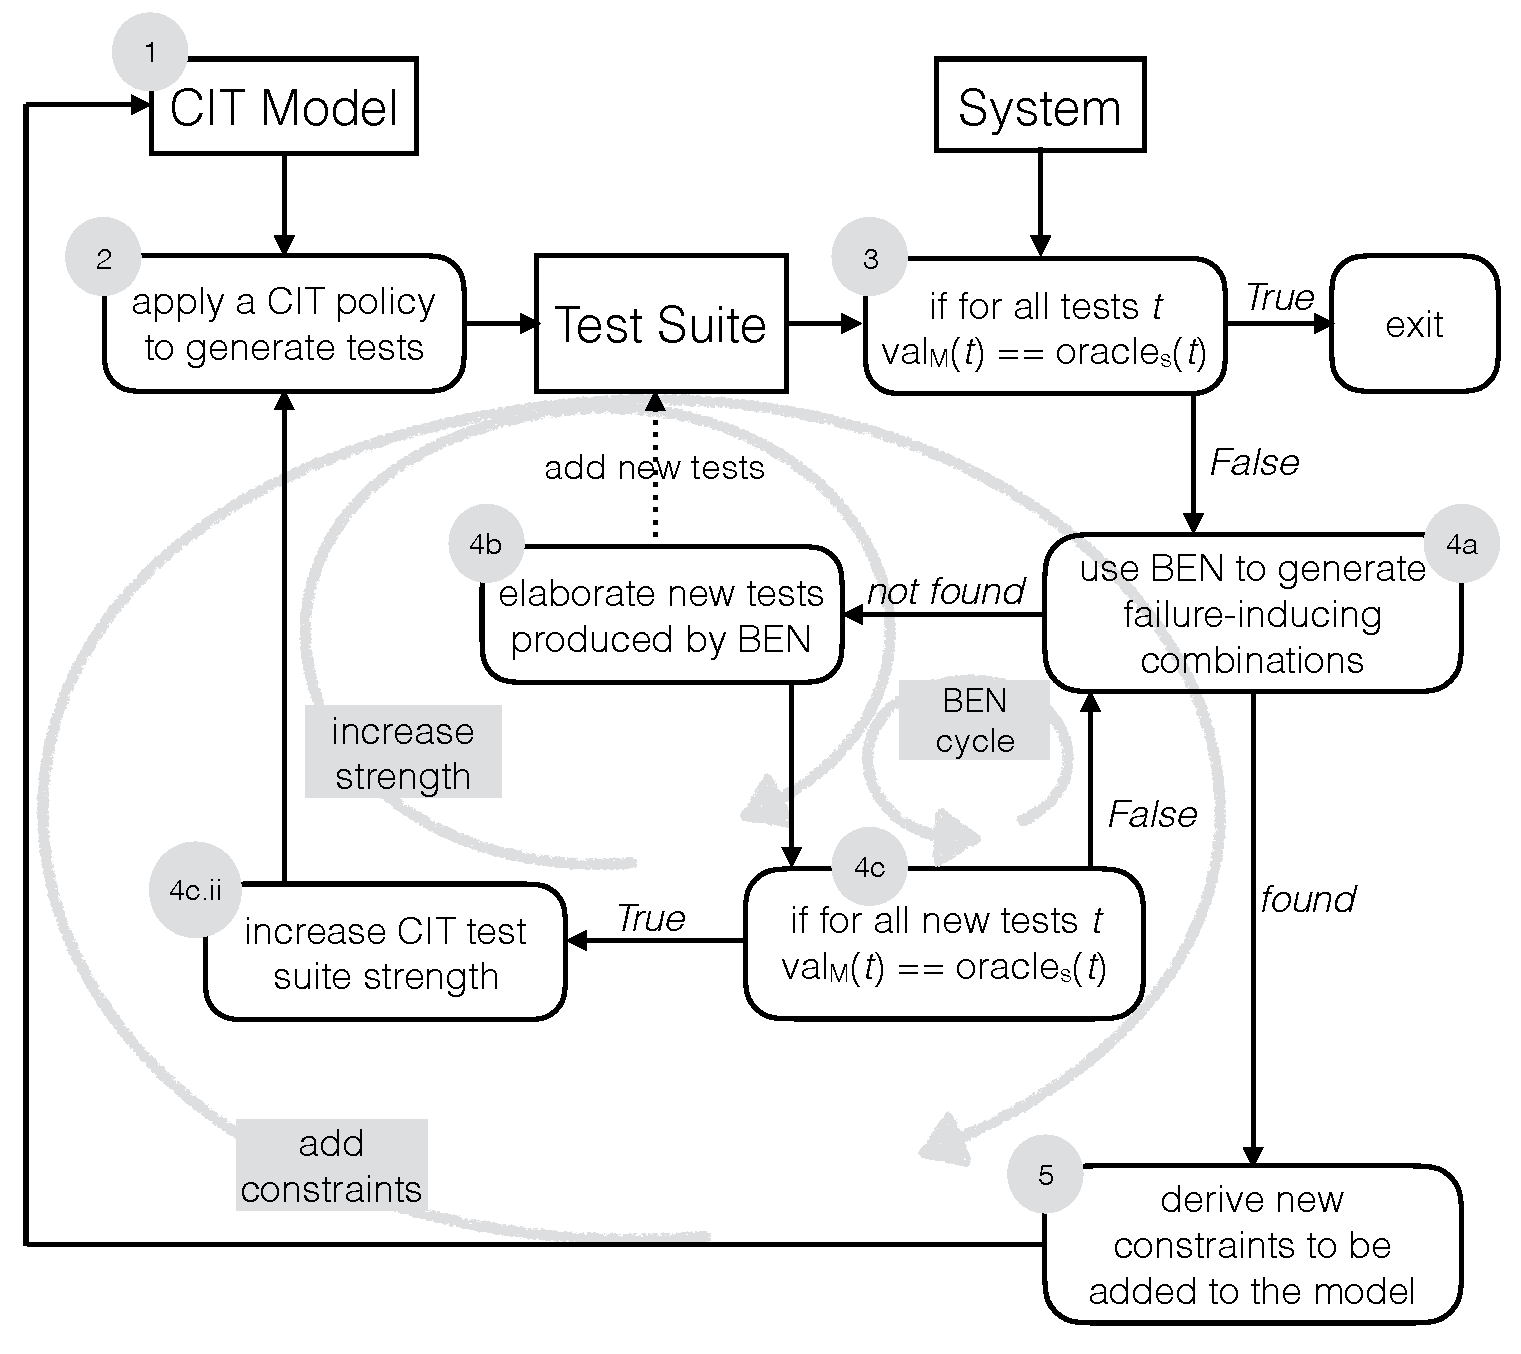
\includegraphics[width=.7\columnwidth]{images/constraintsrepair3.pdf}
	\caption{The constraint repair process.}\label{fig:constraintsrepair}
	\label{fig:repair}
\end{figure}

\bb Taking the exhaustive test suite as $T$, we can compute an absolute failure index ($\mathsf{afi}$) as measure of the quality of a model. However, computing the absolute failure index $\mathsf{afi}$ is infeasible in general. In the experiments, we will be able to compute the models $\mathsf{afi}$ by assuming that we know the exact model of the system. We use multi-valued decision diagrams (MDDs) \cite{hvc14} in order to calculate the number of tests that are permitted by the constraints in the model.\be

\subsection{The constraint repair process}\label{sec:constr_repair}

\bb In this section we present the proposed process for constraint repair in CIT models. In our previous work \cite{Gargantini16:validation} we devised a way of finding conformance faults. We use these techniques to find faults and extend them by proposing an automated way of fixing the faults found.  
Figure \ref{fig:repair} presents an overview of the constraint repair process.


We first generate a set of test cases of given strength $k$ based on one of the CIT policies described in Section \ref{sec:citpolicies}. We evaluate each of the tests $t$ using the function $val_{M}(t)=\mathit{oracle}_{S}(t)$. We mark each test for which $val_{M}(t)\neq\mathit{oracle}_{S}(t)$ as a failing one (since it reveals a conformance fault). We say that the test $t$ passes, otherwise. 

We input the generated test suite and the result of $val_{M}(t)=\mathit{oracle}_{S}(t)$ for each test $t$ into a combinatorial testing-based fault localisation tool called BEN \cite{ben_2015}. BEN uses a heuristic approach to identify a set of failure-inducing combinations of given size (i.e., combinatorial strength) or larger. Given an initial test suite and the result for each test, it identifies a set of suspicious parameter-value combinations. Next, it proceeds in an iterative manner: it generates a set of new tests and queries the user for the result of these tests; after the user supplies the data, BEN identifies a new set of suspicious combinations and a new set of tests; the process is repeated until a set of failure-inducing combinations is found or all tests pass (in which case we can increase the strength of CIT testing)\footnote{In our experiments we also found there are other cases when BEN terminates. These are, however, usually error states. We treat these cases the same way in which we deal with the `all test pass' case, that is, we report that BEN did not find any failure-inducing combinations of given strength.}.
Further details about the heuristic approach implemented in BEN can be found in the following paper: \cite{ben_2015}.
We note that the problem of finding minimum failure-inducing combinations is a challenging task, since generation of an exhaustive test suite is often infeasible. 

Once failure-inducing combinations are found, we modify the constraints of the original CIT model, as explained in Examples \ref{ex:constraining} and \ref{ex:relaxing}. We repeat the whole process until all test cases (generated by the CIT policy of choice and BEN) pass. 

Our proposed constraint repair process proceeds as follows:
\begin{enumerate}
	\item Start with a constrained CIT model containing a set of constraints $C$.
	\item Derive a $t$-way CIT test suite according to one of the CIT policies described in Section~\ref{sec:citpolicies}.
	\item If for all test cases, the test result is the same according to the model and according to the system, then exit.
	\item For all tests $t$ such that $val_M(t) \neq \mathit{oracle}_{S}(t)$, mark $t$ as a failing test. $t$ is passing otherwise. Use BEN to derive failure-inducing combinations:
	\begin{enumerate}
		\item Produce an initial set of suspicious combinations with new test cases using BEN.
		\item Add tests produced by BEN to the test suite. 
		\item Mark the new test cases as failing or passing according to $val_{M}=\mathit{oracle}_{S}$.
		\begin{enumerate}
			\item If all new tests pass and BEN has not detected any failure-inducing combinations, increase the test suite strength. %(Justyna: need to check if BEN can produce failure-inducing combinations even if all new tests pass).
			\item Otherwise, input the new set of tests to BEN.
		\end{enumerate}
		\item If BEN terminates and produces a set of failure-inducing combinations, exit BEN.
	\end{enumerate}
	\item Modify the constraint set $C$ based on the result produced by BEN: \\
	Given the set of failure-inducing combinations $comb$s, for each $comb$:
	\begin{enumerate} 
		\item If a failure-inducing configuration $comb$ occurs in test cases for which $val_M(t)=\mathit{True}$ and $\mathit{oracle}_{S}(t)=\mathit{False}$ (i.e., belongs to the constraining set), then $\mathit{Constr}\leftarrow \mathit{Constr} \cup \neg comb$.
		%\red{A: or using sets?}$C\leftarrow C \cup \{\neg comb\}$
		\item If a failure-inducing configuration $comb$ occurs in test cases for which $val_M(t)=\mathit{False}$ and $\mathit{oracle}_{S}(t)=\mathit{True}$ (i.e., belongs to the relaxing set), then for each $c_i \in \mathit{Constr}$, add $comb$ to $c_i$, that is, $c_i \leftarrow c_i \vee comb$.
	\end{enumerate}
	\item Go back to point 1. 
\end{enumerate}



Note that this approach can be used to infer constraints by supplying an unconstrained CIT model to our tool. 

The final constraints produced by our process can be further simplified. Since constraints in our model can be represented in Boolean form, we can use propositional logic rules. We leave this step as future work. 

Another enhancement would be identification of constraints to which $comb$s from the relaxing set need to be added. However, identification of the set of constraints that violate a $comb$ is a non-trivial task. It can be reduced to the problem of finding minimum unsatisfiable sets in Boolean satisfiability solving (SAT). We leave this step as future work.\be

\subsection{Experiments}\label{sec:constr_experiments}

\bb In order to test our approach we conducted the following two experiments\footnote{All the experiments have been executed on a Linux PC with two Intel(R) i7-3930K CPU  (3.2 GHz) and 16 GB of RAM.}. In the first experiment, we applied mutation to a set of models taken from the literature. In the second experiment, we used a configurable software system, namely Django, in order to test our framework on a real case study.\be


\subsubsection{Mutation Analysis}

\bb
We gathered a set of combinatorial models taken from several papers and applied our process to mutated versions of these models. In particular, for every model $m$ in the benchmarks we derived a set $M$ of mutants.

We have applied simple mutation operators to the constraints in the model under test in order to find  mutants to be repaired. Our mutation operators are of 4 types: add a constraint that excludes a value of a parameter, remove an entire constraint, negate a constraint, and change a logical operator to another one (\emph{AND} to \emph{OR} etc.).   Then, for each mutant $m'$ in $M$, representing a possible faulty model,  we applied our repair process by using the original model $m$ as the oracle (to compute the $\mathit{oracle}_S$ function). 

We considered all CIT policies presented Section \ref{sec:citpolicies}. We applied our repair starting with combinatorial strength set to 1 and increase it up to 3 (i.e., we are only concerned with finding failure-inducing combinations of size 1,2 and 3). We included combinatorial tests of strength 1 since some faults can be already detected by a single parameter assignment.
\be

\subsubsection{Benchmarks}

\bb We used 5 case studies to evaluate our proposed approach:

\begin{asparaenum}
	
	\item The \textbf{WashingMachine} system, model of which is presented in Figure \ref{fig:washerexample}. It represents an abstract view of the human interaction with an \emph{embedded system}.  
	
	\item \textbf{Concurrency} is a testing problem for real-life concurrent system presented in \cite{segall_using_2011}.
	
	\item \textbf{Telecom} is a real-life telecommunication system presented in \cite{segall_using_2011}.
	
	\item \textbf{Aircraft} is a small Software Product Line (SPL) found in SPLOT repository and presented in \cite{Voelter:2009}.
	
	\item \textbf{Libssh} is the combinatorial model for cmake of SSH library taken from \cite{icst2016}.
		
\end{asparaenum}
\be

\begin{table}[h]
	\caption{The benchmark data {\small (for CNF size $a^b$ means $b$ clauses with $a$ literals each.)}}\label{tab:constr_benchmarks}
	\small \centering
	\resizebox{.8\columnwidth}{!}{
		\begin{tabular}{p{15mm}rrrrrr|r}
			\toprule
			& & \multicolumn{2}{c}{constraints} & \multicolumn{2}{c}{State space} & validity &mut-\\
			\cline{3-4} \cline{5-6} 
			name & \#var & \# & CNF size & exp & \#conf & ratio &ants\\ 
			\midrule
			WashingM. & 3 & 2 & $2^{3}$ & $2^{1}3^{2}$ & 18& 66\% & 18\\ 
			Concurrency	& 5	 & 7 &	$2^{4}3^{1}5^{2}$ &	$2^{5}$	& 32 & 25\% & 38 \\ 	
			Aircraft &	8 &	2 &	$3^{1}4^{1}$ &	$2^{7}3^{1}$ &	384&  82\% & 25\\	
			Libssh & 16 & 2 & $2^{2}$ & $2^{16}$ & 65536  & 50\% & 42\\ 
			Telecom	& 10& 21 & $2^{11}3^{1}4^{9}$	& $2^{5}3^{1}4^{2}5^{1}6^{1}$	& 46080	& 39\% & 116\\
			\bottomrule
		\end{tabular}
	}
\end{table}

\smallskip

\bb Table \ref{tab:constr_benchmarks} presents various benchmark data: number of variables, number of constraints (including the number of clauses when converted to conjunctive normal form (CNF)), the size of the state space (the total number of possible configurations), and the percentage of configurations that are valid  (i.e. the ratio of valid configurations). Note that a low ratio indicates that there are only few valid configurations. We tried to collect models from different domains, with a good level of diversity (in terms of size, constraints, and so on) in order to increase the validity of our findings.

We ran each constraint repair process 10 times and report averages. We used the ACTS tool for CIT test suite generation.

Table \ref{tab:constr_benchmarks} reports the number of mutants we generated for each model.\be

\begin{figure*}
	\centering
	\begin{subfigure}[b]{0.49\textwidth}
		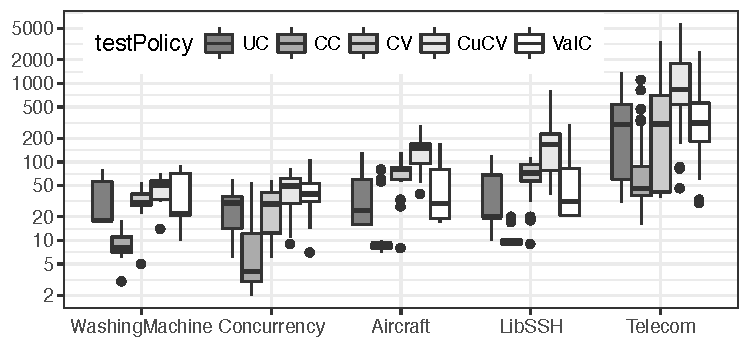
\includegraphics[width=0.98\textwidth]{data/initTests.pdf}
		\caption{Tests}\label{fig:initTests}
	\end{subfigure}
	\begin{subfigure}[b]{0.49\textwidth}
		\centering
		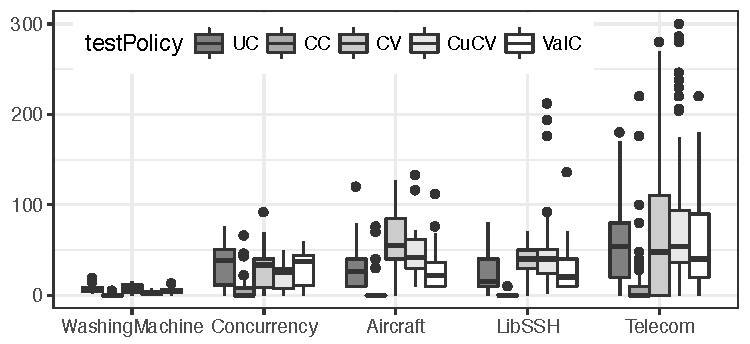
\includegraphics[width=0.98\textwidth]{data/BENTests.pdf}
		\caption{BEN (additional tests)}\label{fig:ben}
	\end{subfigure}
	\begin{subfigure}[b]{0.49\textwidth}
		\centering
		
\includegraphics[width=0.98\textwidth]{data/oraclecalls.pdf}
		\caption{Oracle (number of oracle calls)}
	\end{subfigure}
	\begin{subfigure}[b]{0.49\textwidth}
		\centering
		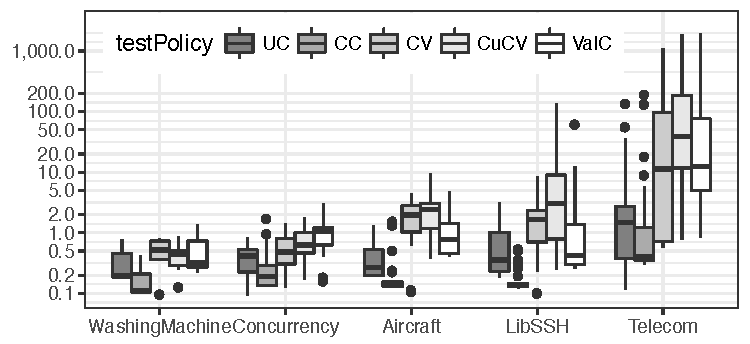
\includegraphics[width=0.98\textwidth]{data/time.pdf}
		\caption{Time (seconds)}\label{fig:time}
	\end{subfigure}
	\caption{Effort of the repair process}\label{fig:repaireffort}
\end{figure*}

\subsection*{Evaluation of Effort and Repair Capability by mutation} 

\bb In order to evaluate our technique,  we wanted first to measure the required \emph{effort} and how it varies by changing the CIT policy. To measure the effort we used, for each mutant:

\begin{compactdesc}
	\newcommand{\Time}{\textbf{Time}\xspace}
	\newcommand{\Ben}{\textbf{BEN}\xspace}
	\newcommand{\Tests}{\textbf{Tests}\xspace}
	\newcommand{\Oracle}{\textbf{Oracle}\xspace}
	\item[\Tests] The number of test cases are generated according to the given testing policy. Note that for a mutant, test case generation can be invoked several times.
	\noindent This can happen if, e.g., not all the tests pass and BEN is not able to find the failure-inducing combination and we have to increase the combinatorial testing strength.
	
	\item[\Ben] The number of additional tests BEN requires in order to isolate the failure-inducing combinations. 
	
	\item[\Oracle] The number of times the oracle was called.
	
	\item[\Time] The total time required to fix a mutated model, including test generation, BEN invocation, and oracle evaluation. 
\end{compactdesc}

In this experiment, the time required by the oracle to evaluate a test is negligible, since we use the original model as an oracle. However, for real software systems a single invocation of the 	oracle may take several minutes. Thus the number of oracle calls is 	the critical factor as the evaluation of the function $\mathit{oracle}_{S}$ can be 	expensive, especially if human input is required.

\smallskip
\noindent We are also interested in assessing the \emph{repair capability} of our approach. We use the following two measures:
\be

\begin{compactdesc}
	
	\newcommand{\TRM}{\textbf{TRM}\xspace}
	\newcommand{\FID}{\textbf{FID}\xspace}
	
	\item[\TRM\ -- Totally Repaired Models.] The ratio of completely repaired models. 
	%if, given a mutant, the process was able to obtain a totally repaired model. 
	In this experiment, we can check if a repaired model is completely fault free by querying whether it is equivalent to the original  model. To check equivalence among combinatorial models we use an SMT solver \cite{Arcaini2014}.
	
	\item[\FID\ -- Failure Index Delta.] Even if a model is not completely repaired, we are interested in measuring how many conformance faults were repaired. We define $\mathrm{FID} = (\mathsf{afi}_{init} - \mathsf{afi}_{final})/\mathsf{afi}_{init}$ in terms of the absolute failure index presented in Def. \ref{def:failureindex}. FID represents the percentage of conformance faults that are repaired.
	
\end{compactdesc}

\begin{figure*}
	\centering
	\begin{subfigure}[b]{0.49\textwidth}
		\centering
		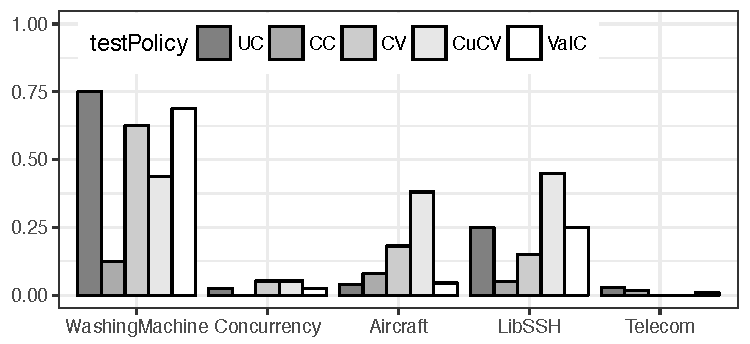
\includegraphics[width=0.98\textwidth]{data/TRM.pdf}
		\caption{\footnotesize TRM: Totally repaired models (over all the mutations)}\label{fig:TRM}
	\end{subfigure}
	\begin{subfigure}[b]{0.49\textwidth}
		\centering
		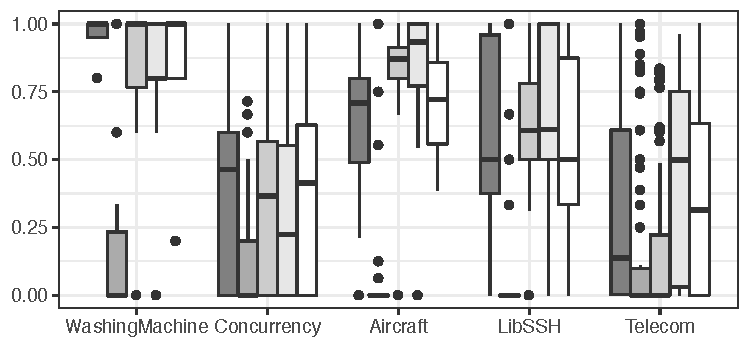
\includegraphics[width=0.98\textwidth]{data/FID.pdf}
		\caption{\footnotesize FID: Failure Index Delta}\label{fig:FID}
	\end{subfigure}
	\caption{Repair capability}\label{fig:repaircapability}
\end{figure*}

\begin{table*}[h]
	\setlength{\tabcolsep}{3pt}
	\caption{Means of the quantities over all the mutations}\label{tab:constr_results}
	\resizebox{\textwidth}{!}{
		\begin{tabular}{lrrrrr|rrrrr|rrrrr|rrrrr}
			\toprule
			&  \multicolumn{5}{c}{Time (seconds)} & \multicolumn{5}{c}{Tests (Initial)} & \multicolumn{5}{c}{BEN (additional tests)} &\multicolumn{5}{c}{FID (\%)}\\
			%\cline{2-6} \cline{8-12} \cline{13-15} \cline{17-20}
			name & 
			\multicolumn{1}{c}{UC} &  \multicolumn{1}{c}{CC}& \multicolumn{1}{c}{CV}& \multicolumn{1}{c}{CuCV}& \multicolumn{1}{c}{ValC}& \multicolumn{1}{c}{UC} &  \multicolumn{1}{c}{CC}& \multicolumn{1}{c}{CV}&\multicolumn{1}{c}{CuCV}& \multicolumn{1}{c}{ValC}& \multicolumn{1}{c}{UC} &  \multicolumn{1}{c}{CC}&\multicolumn{1}{c}{CV}&\multicolumn{1}{c}{CuCV}& \multicolumn{1}{c}{ValC}& \multicolumn{1}{c}{UC} & \multicolumn{1}{c}{CC}& \multicolumn{1}{c}{CV}&\multicolumn{1}{c}{CuCV}& \multicolumn{1}{c}{ValC}\\ 
			\midrule
			WashingM. & 
			0.3 & 0.2 & 0.5  & 0.4   & 0.5   & 31.5  & 9.6   & 29.7  & 45.0   & 36.3  &  6.6  & 0.6  & 6.5  & 2.5  & 4.6  & 95 & 21 & 81 & 82 & 86 \\
			Concurrency	& 
			0.4 & 0.3 & 0.6  & 0.8   & 1.1   & 27.8  & 11.3  & 29.1  & 47.0   & 41.9  &  33.0 & 8.0  & 29.9 & 20.7 & 30.8 & 36 & 13 & 33 & 29 & 36 \\
			Aircraft &
			0.4 & 0.3 & 2.0  & 2.9   & 1.3   & 41.1  & 18.1  & 74.0  & 144.5  & 51.6  &  33.3 & 8.6  & 59.5 & 50.4 & 31.5 & 62 & 14 & 79 & 85 & 60 \\
			Libssh &
			0.7 & 0.2 & 1.8  & 77.9  & 2.6   & 44.0  & 10.8  & 66.5  & 187.5  & 54.6  &  23.4 & 1.0  & 35.3 & 46.3 & 26.0 & 57 & 10 & 63 & 67 & 50 \\
			Telecom	& 
			4.5 & 4.0 & 83.0 & 180.3 & 107.7 & 352.1 & 111.8 & 532.1 & 1287.0 & 435.9 &  56.1 & 11.5 & 70.0 & 77.6 & 60.1 & 25 & 16 & 12 & 35 & 31\\
			\bottomrule
		\end{tabular}
	}
\end{table*}


\bb Figures~\ref{fig:repaireffort} and \ref{fig:repaircapability} show respectively the effort and  the repair capability of each policy for every model in the benchmark set. The experimental results are also summarized in Table~\ref{tab:constr_results}. 

We can observe that the number of tests generated at the beginning of each repair process (Fig.~\ref{fig:initTests}) and the number of tests BEN requires in order to find failure-inducing combinations (Fig.~\ref{fig:ben}) are correlated.  If one starts with small test suites, BEN will require fewer tests (and it likely identifies fewer failure-inducing combos).  In terms of time (Fig.~\ref{fig:time}), our process is rather fast for small models, but also for the biggest models, like Telecom, it terminates on average in less than 10 seconds for weak policies (like \ic and \ccit), and in any case in less than 10 minutes when using strong policies like \cucv and \ValC.
Regarding the repair capability, the TRM is rather small for big specifications, and using more powerful testing policy (like CuCV) does not help much (Fig.~\ref{fig:TRM}). Using our process to obtain a completely bug-free model seems unrealistic for big models: CIT likely provides an insufficient coverage for this. 
However, if we consider  the FID in Fig.~\ref{fig:FID}, we can say that almost always our technique and CIT improve the model except when using CC. The overall minimum average for FID when using strong policies like CuCV and ValC is 29\%. For big models, there are cases in which we are unable to improve the constraints, but on average we can still remove around 35\% of the faults with CuCV and ValC. As already observed in \cite{Gargantini16:validation}, the CC policy (that generates only valid tests) detects fewer conformance faults, and for this reason has the lowest FID. The average FID over all the mutants is around 37\%. The average FID when using CuCV is 49\%: half of faults can be repaired on average if the user chooses this policy.\be

\subsubsection{Repairing the model of Django parameters}

\bb \textbf{Django} is a free and open source web application framework, written in Python, that supports the creation of complex, database-driven websites, emphasizing reusability of components\footnote{\url{https://www.djangoproject.com/}}. Each Django project has a configuration file. 

\noindent It is loaded at \emph{launch time}, i.e. every time the web server that executes the project (e.g. Apache) is started.
Among all the possible configuration parameters, we selected and modelled one Enumerative and 23 Boolean parameters. We implemented an automated oracle which returns true if and only if the HTTP response code of the Django project homepage is 200 (HTTP OK). This oracle invocation is costly in terms of time, since editing the settings of the Django project, starting the Apache server, and waiting for its response, requires around 6 seconds.

We applied the constraint repair process described in Section~\ref{sec:repair} on a default Django start project running on Apache server (without SSL configuration) called at address \emph{localhost}. We started from a model (Django0) with an empty set of constraints because we thought that Django was accepting (and amending if necessary) every possible configuration, and secondly, to test the effectiveness of this technique to \emph{infer} (and not only \emph{repair}) configuration constraints: we call this first experiment "\textsf{Inference from Django0}".
At the end of the process, we obtained different set of constraints depending on the policy.
For all the policies, we executed the repair process with test suite strength from 1 to 3.

We noticed that the application of the testing policy \cv produces an empty test suite at the beginning, and an empty set of constraints at the end of the process, because the initial Django model contains no constraints, and in particular there are no test cases violating constraints. So we ignored this policy in the experiments.

We manually derived the constraints, based on the Django documentation about configuration files, and by looking at the results of a few test cases. As a second experiment, we applied the constraint repair process to this manual model (\textsf{Manual}), in order to improve its conformance with the real Django system: we call this second experiment "\textsf{Repairing Manual}".\be

\begin{table}[H]
	\begin{minipage}{\columnwidth} % used to display footnotes: http://tex.stackexchange.com/questions/51454/footnotes-tabularx-environment-latex
		\caption{Django inference and repair results}\label{tab:djangoresults}
		\centering
		\resizebox{0.8\columnwidth}{!}{	
			\centering
			\begin{tabular}{llrrrrrrr}
				\toprule
				&Policy & Tests & BEN & Oracle & Time & C\footnote{C: Total number of constraints in the model} & P\footnote{P: Total number of parameters involved in the constraints (without considering duplicates)} & fi \\%& Over-constr. \\ 
				\midrule
				\multicolumn{6}{l}{Django0 (empty model)}  & 0 & 0 & 0.789 \\%& 0\% \\\midrule
				\midrule
				\multirow{4}{*}{\rotatebox[origin=c]{90}{\parbox[c]{1.5cm}{\centering inference from Django0}}} 
				& \ic & 36 & 20 & 32 & 201s & 5 & 6 & 0.325 \\%& 0.342\% \\
				& \ccit & 173 & 60 & 154 & 1671s & 8 & 9 & 0.254 \\%& 0\% \\
				& \cucv & 320 & 54 & 335 & 3570s & 9 & 12 & \cellcolor{light-gray}0.081 \\%& 0\% \\ 
				& \ValC & 288 & 80 & 124 & 1453s & 17 & 19 & 0.204 \\%& 0.057\% \\ 	
				%\CCi & 621 & 100 & 116 & 1100.802s & \\
				\midrule
				\multicolumn{6}{l}{Manual} & 3 & 4 & 0.033 \\%& 0\% \\
				\midrule
				\multirow{4}{*}{\rotatebox[origin=c]{90}{\parbox[c]{1.5cm}{\centering repairing Manual}}} 
				& \ic & 63 & 30 & 51 & 435s & 3 & 4 & 0.033 \\%& 0.342\% \\
				&\ccit & 63 & 30 & 70 & 436s & 3 & 4 & 0.033 \\%& 0\% \\
				&\cucv & 202 & 30 & 167 & 1354s & 4 & 4 & \cellcolor{light-gray}0 \\%& 0\% \\ 
				&\ValC & 118 & 30 & 92 & 564s & 4 & 4 & \cellcolor{light-gray}0 \\%& 0.057\% \\ 	
				\bottomrule
			\end{tabular}
	}\end{minipage}
\end{table}

\bb Results of this experiment are summarized in Table~\ref{tab:djangoresults}, which reports the number of tests generated by the testing policy, the number of additional tests required by BEN, the number of oracle calls, the time taken for the whole process, the number of constraints of the final model, the number of parameters involved in the constraints, and the failure index. 
To compare the different policies in terms of fault detection capability, in this case, we cannot rely on the absolute failure index, since the actual model of the Django system remains unknown. We can, however, compute the failure index (see Definition~\ref{def:failureindex}) % by considering 
where the test suite $T$ is the union of all the test suites we generated for all the policies. 

%Regarding the \emph{inferring} problem, as expected,

With regards to \emph{inferring} constraints,  the \cucv policy generates the biggest test suite and requires also the largest amount of time: around 1h for constraint inference from {\sf Django0} (including oracle invocation). It has also the lowest {\sf fi} (8\%), which however is not zero: no inferred model is completely fault-free. The \ic policy is the worst in terms of failure index data, but it is the fastest in our experiment.

\noindent \ValC produces a model with the largest number of constraints and the failure index (20\%) is the second lowest. %not satisfactory. 
However, if we compare the failure index of Diango0 (79\%), we can say that all the testing policies can substantially improve the initial empty model. In conclusion, all the models contain a reasonable number of constraints and although our best policy (\cucv) does not beat the manual model we have developed (by using our best efforts), it can produce a rather correct model.  

Regarding the problem of \emph{repairing}  the initial manual model, two out of four testing policies (\cucv and \ValC) are able to completely repair the manual model (at least when considering the failure index based on the set of generated tests), while the \ic and \ccit policies did not improve the initial model.  For constraint repair, the number of tests and the time required is generally lower (except for \ic) than for the process of inferring constraints. We conclude that the availability of an initial model, even if it is not completely correct, makes possible to obtain a fault-free model for a real system when strong testing policies are applied.

Figure~\ref{fig:djangofaults} reports the constraints for \textsf{Django0} (the initial model with empty set of constraints), \textsf{Manual} (the model \emph{inferred} manually), and for the repaired models produced using \cucv and \ValC (starting from \textsf{Manual}). % The inferred constraints are shown in Figure~\ref{fig:djangofaults}. 
The constraints obtained in the final models are still readable, making a human inspection possible for further modifications.  \be


\begin{figure}[h]
	\lstset{language=comb,basicstyle=\fontsize{7.5}{8}\sffamily,frame=single,columns=flexible}
	\begin{lstlisting}
	Django0
	# true #
	\end{lstlisting}
	\begin{comment}
	\vspace{-3mm}
	\begin{lstlisting}
	UC:
	# SESSION_EXPIRE_AT_BROWSER_CLOSE => !SECURE_SSL_REDIRECT #
	# USE_TZ => !SECURE_SSL_REDIRECT #
	# SECURE_CONTENT_TYPE_NOSNIFF => SECURE_SSL_REDIRECT #
	# USE_X_FORWARDED_HOST => SECURE_SSL_REDIRECT #
	# USE_ETAGS => SECURE_SSL_REDIRECT #
	\end{lstlisting}\vspace{-3mm}
	\begin{lstlisting}
	CC:
	# SESSION_EXPIRE_AT_BROWSER_CLOSE => !SECURE_SSL_REDIRECT #
	# USE_TZ => !SECURE_SSL_REDIRECT #
	# USE_L10N => !PREPEND_WWW or SESSION_COOKIE_HTTPONLY #
	# !DEBUG_PROPAGATE_EXCEPTIONS => !USE_L10N or !PREPEND_WWW #
	# !DEBUG_PROPAGATE_EXCEPTIONS => !PREPEND_WWW or SESSION_COOKIE_HTTPONLY #
	# PREPEND_WWW => !SESSION_COOKIE_SECURE or SESSION_COOKIE_HTTPONLY #
	# PREPEND_WWW => SESSION_COOKIE_HTTPONLY or !SECURE_CONTENT_TYPE_NOSNIFF #
	# DEBUG_PROPAGATE_EXCEPTIONS => !PREPEND_WWW or !SESSION_COOKIE_HTTPONLY #
	\end{lstlisting}\vspace{-3mm}
	\begin{lstlisting}
	CuCV:
	# SESSION_EXPIRE_AT_BROWSER_CLOSE => !SECURE_SSL_REDIRECT #
	# USE_TZ => !SECURE_SSL_REDIRECT #
	# USE_L10N => !PREPEND_WWW or SECURE_SSL_REDIRECT #
	# PREPEND_WWW => SESSION_COOKIE_HTTPONLY or SECURE_SSL_REDIRECT #
	# PREPEND_WWW => !SESSION_COOKIE_SECURE or SECURE_SSL_REDIRECT #
	# !DEBUG_PROPAGATE_EXCEPTIONS => !PREPEND_WWW or SECURE_SSL_REDIRECT #
	# PREPEND_WWW => SESSION_SAVE_EVERY_REQUEST or SECURE_SSL_REDIRECT #
	# !USE_TZ => SESSION_EXPIRE_AT_BROWSER_CLOSE or !SECURE_SSL_REDIRECT #
	# ALLOWED_HOSTS==IP => PREPEND_WWW or SECURE_SSL_REDIRECT #
	\end{lstlisting}\vspace{-3mm}
	\begin{lstlisting}
	ValC:
	# !DEBUG => USE_I18N or !SECURE_SSL_REDIRECT #
	# !DEBUG => !SECURE_HSTS_INCLUDE_SUBDOMAINS or !SECURE_SSL_REDIRECT #
	# !DEBUG => SESSION_EXPIRE_AT_BROWSER_CLOSE or !SECURE_SSL_REDIRECT #
	# !DEBUG => DEBUG_PROPAGATE_EXCEPTIONS or !SECURE_SSL_REDIRECT #
	# !DEBUG => EMAIL_USE_SSL or !SECURE_SSL_REDIRECT #
	# ALLOWED_HOSTS==IP => !DEBUG or CSRF_COOKIE_HTTPONLY #
	# ALLOWED_HOSTS==IP => !DEBUG or USE_ETAGS #
	# ALLOWED_HOSTS==IP => !DEBUG or !USE_THOUSAND_SEPARATOR #
	# ALLOWED_HOSTS==IP => !DEBUG or !APPEND_SLASH #
	# DEBUG => !PREPEND_WWW or !SECURE_CONTENT_TYPE_NOSNIFF #
	# !DEBUG => !PREPEND_WWW or SECURE_SSL_REDIRECT #
	# ALLOWED_HOSTS==NONE => USE_I18N or SESSION_COOKIE_HTTPONLY #
	# ALLOWED_HOSTS==NONE => USE_L10N or SESSION_COOKIE_HTTPONLY #
	# ALLOWED_HOSTS==NONE => USE_TZ or SESSION_COOKIE_HTTPONLY #
	# ALLOWED_HOSTS==NONE => SESSION_COOKIE_HTTPONLY or SECURE_CONTENT_TYPE_NOSNIFF #
	# ALLOWED_HOSTS==IP => SESSION_COOKIE_SECURE or SESSION_COOKIE_HTTPONLY #
	# ALLOWED_HOSTS==LOCALHOST => !CSRF_COOKIE_HTTPONLY or !SECURE_SSL_REDIRECT #
	\end{lstlisting}
	\end{comment}
	\vspace{-3mm}
	\begin{lstlisting}
	Manual (constraints "inferred" manually)
	# !PREPEND_WWW #
	# !SECURE_SSL_REDIRECT #
	// if not DEBUG, "localhost" must be allowed
	# !DEBUG => 
	(ALLOWED_HOSTS==LOCALHOSTIP or ALLOWED_HOSTS==LOCALHOST) #
	\end{lstlisting}
	\vspace{-3mm}\begin{lstlisting}
	CuCV (repairing Manual)
	# !PREPEND_WWW #
	# !SECURE_SSL_REDIRECT #
	# !DEBUG => 
	ALLOWED_HOSTS==LOCALHOSTIP or ALLOWED_HOSTS==LOCALHOST #
	# ALLOWED_HOSTS==IP => 
	!DEBUG or PREPEND_WWW or SECURE_SSL_REDIRECT #
	\end{lstlisting}
	\vspace{-3mm}\begin{lstlisting}
	ValC (repairing Manual)
	# !PREPEND_WWW #
	# !SECURE_SSL_REDIRECT #
	# !DEBUG => 
	ALLOWED_HOSTS==LOCALHOSTIP or ALLOWED_HOSTS==LOCALHOST #
	# ALLOWED_HOSTS==IP => !DEBUG or SECURE_SSL_REDIRECT #
	\end{lstlisting}
	\caption{Django models obtained by repairing the manual model using different testing policies}\label{fig:djangofaults}	
	
\end{figure}


	\subsection{Related Work}
\label{sec:validation_relatedwork}

\bb The problem of modelling and testing the configurability of complex systems is non-trivial. There has been much research done in extracting constraints among parameter configurations from real systems (problem space) and modelling system configurability \cite{ShiCD12,henard_towards_2013,YilmazDCP14}.
For instance, the importance of having a model of variability and having the constraints in the model aligned with the implementation is discussed in \cite{NadiBKC14}. However, in that paper, authors try to identify the sources of configuration constraints and to automatically extract the variability model. Our approach is oriented towards the validation of a variability model that already exists. Moreover, they target C-based systems that realise configurability with their build system and the C preprocessor. 
A similar approach is presented in \cite{Tartler:2011}, where authors extract the compile-time configurability from its various implementation sources and examine for inconsistencies (e.g., dead features and infeasible options). We believe that our approach is more general (not only compile-time and C-code) and can be complementary used to validate and improve automatically extracted models. 

Testing configurable systems in the presence of constraints is tackled in \cite{CohenTSE08} and \cite{Petke15:practical}. In these papers, authors argue that CIT is a very efficient technique and that constraints among parameters should be taken into account in order to generate only valid configurations. This allows to reduce the cost of testing. Also in \cite{jar10}, authors have shown how to successfully deal with the constraints by solving them by using a constraint solver such as a Boolean satisfiability solver (SAT). However, the emphasis of that research is more on testing of the final system not its model of configurability. CIT is also widely used to test SPLs \cite{Perrouin010a}.

In SPL the validation and extraction of constraints between features is generally  given in terms of feature models (FMs). Synthesis of FMs can be performed by identifying patterns among features in products and in invalid configurations and build hierarchies and constraints (in limited form) among them. For instance, Davril et al. apply feature mining and feature associations mining to informal product descriptions~\cite{Davril13}. There exist several papers that apply search based techniques, which generally give better results~\cite{SBSEforSPLsurvey,LopezHerrejon201533,FerreiraVQ13,lopez-herrejon_reverse_2012}. However, checking and maintaining the consistency between a SPL and its feature model is still an open problem. A preliminary proposal is presented in \cite{icst2016}, which however does not use CIT but a more complex logic based approach. We plan to compare our approach with \cite{icst2016} in order to check if CIT can provide benefits in terms of easiness in test generation and shorter  generation times.\be



\subsection{Related Work}
\label{sec:constr_relatedwork}

%%%%%% Added by Justyna
\bb The problem of finding and fixing constraints in combinatorial models has been addressed in the field of software product lines. Henard et al. \cite{henard_towards_2013} assumes existence of valid configurations of the given software system and use a SAT solver to randomly generate configurations for an existing feature model of the system. Once a conformance fault is found, a constraint is added, removed or altered with certain probability. The mutated feature model is compared against the original using a pre-defined fitness function and the best of the two is kept for future evaluation. 

In contrast to Henard et al.'s work, we derive test cases in a systematic fashion using combinatorial interaction testing. Moreover, by applying policies presented in \cite{Gargantini16:validation}, we are able to generate invalid configurations. Therefore, in contrast to the work by Henard et al., we are able to find conformance faults caused by an over-constrained model. Finally, we use a systematic approach to fix the model by utilising BEN to find the minimum fault-inducing configurations.

Some of our policies could be improved by integrating the \emph{testing with negative values} technique described in~\cite{czerwonka2006pairwise}, which disallows two \emph{invalid values} to coexist in one test case (negative test cases), assuming that every configuration containing at least one invalid parameter is invalid. We did not consider that technique because it does not apply to the more general case (which is quite common) of invalid configurations originating from \emph{t-way} parameter interactions. A possible future work is to modify our \cv and \ValC policies to include only configurations that make \emph{exactly} one constraint false.

Arcaini et al. \cite{icst2016} used mutation testing to detect and fix conformance faults by distinguishing a given feature model from its mutants. \be

%%%%%%

The problem of modelling and testing the configurations of complex software systems is non-trivial. There has been much research done in extracting constraints among parameter configurations from real systems. % (problem space).
For instance, the importance of having a model of variability and having the constraints in the model aligned with the implementation is discussed in \cite{NadiBKC14}. However, in that paper, authors try to identify the source of configuration constraints and to automatically extract the variability model. Our approach is oriented towards the validation of a variability model that already exists. Moreover, they target C-based systems that realise configurability with their build system and the C preprocessor. 
A similar approach is presented in \cite{Tartler:2011}, where the authors extract the compile-time configurability from its various implementation sources and examine for inconsistencies (for example, dead features and infeasible options). We believe that our approach is more general (not only compile-time and C-code) and can be complementary in validating and improving automatically extracted models.

Testing configurable systems in the presence of constraints is tackled in \cite{CohenTSE08} and \cite{Petke15:practical}. In these papers, authors argue that CIT is a very efficient technique and that constraints among parameters should be taken into account in order to generate only valid configurations. This allows to reduce the cost of testing. Also in \cite{jar10}, authors showed how to successfully deal with constraints by solving them using a constraint solver such as a Boolean satisfiability solver (SAT). However, the emphasis of that research is more on testing of the final system not its combinatorial model. CIT is also widely used to test SPLs \cite{Perrouin010a}.

In SPL the validation and extraction of constraints between features is generally given in terms of feature models (FMs). Synthesis of FMs can be performed by identifying patterns among features in products and in invalid configurations and build hierarchies and constraints (in limited form) among them. For instance, Davril et al. applied feature mining and feature associations mining to informal product descriptions~\cite{Davril13}. There exist several papers that apply search based techniques, which generally give better results~\cite{SBSEforSPLsurvey,LopezHerrejon201533,FerreiraVQ13,lopez-herrejon_reverse_2012}. However, checking and maintaining the consistency between a SPL and its feature model is still an open problem. 





\section{Using Iterative Constraint Repair to Detect XSS Vulnerabilities}
\begin{tikzborder}{\cite{garn2019}}
We consider the case where a knowledge base consists of interactions among parameter values in an input parameter model for web application security testing.
The input model gives rise to attack strings to be used for exploiting XSS vulnerabilities, a critical threat towards the security of web applications.
Testing results are then annotated with a vulnerability triggering or non-triggering classification, and such security knowledge findings are added back to the knowledge base, making the resulting attack capabilities superior for newly requested input models.
We present our approach as an iterative process that evolves an input model for security testing.
Empirical evaluation on six real-world web application shows that the process effectively evolves a knowledge base for XSS vulnerability detection, achieving on average 78.8\% accuracy.
\be

\subsection{Introduction} \label{sec:intro}
%%% RATIONALE
%%% the rationale provides suf?cient context to justify everything that was done
%\red{RATIONALE: Importance of detecting vulnerability an din particular vulnerability conditions} \blue{partially copied and modified from previous paper}
\bb Computer users of today often interact via web-applications with services offered by various parties.
This new way of connecting the client and server side with each other has brought about a multitude of novel security challenges, both for the client and the server~\cite{catteddu2010cloud}.
One major threat to web applications is posed by Cross-Site Scripting (XSS), which continues to be included in the OWASP Top 10 most critical web application security risks~\cite{owasp17}.
Security testing is a vital and expensive part of the software development lifecycle.
An effective testing technique applied to security testing is \emph{Combinatorial Testing} (CT), for the capability of detecting failures and fail conditions with a small amount of tests that need to be executed compared to the whole input space~\cite{SKVKS2016:IEEEComp}. Given a discrete finite model of the \textit{system under test}
(SUT), made of parameters with a finite list of possible values, called \textit{input parameter model} (IPM), and given an
interaction strength $t$, CT creates a test suite guaranteeing the appearance of all $t$-way interactions of parameter values, for any selection of $t$ parameters~\cite{kuhn2013introductionbook}. 
In the case for testing for exploiting XSS vulnerabilities, the IPM specifies an attack grammar and is also called \textit{(abstract) attack model}.
The aim of this paper is to present a way to evolve knowledge bases for security testing. 
In our approach, the evolution of a knowledge base consists in the integration of learned constraints, using BEN~\cite{ghandehari2018combinatorial}, into the IPM. 
In particular, the contribution of this paper consists in an automated technique to detect all the conditions under which vulnerabilities are triggered, by using combinatorial testing.
Evaluation shows that the process is able to evolve the knowledge base to achieve, on average over all the benchmarks, 78.8\% accuracy, in 14 minutes computation time.

The rest of the paper is structured as follows. In Sect. \ref{sec:xssbasic} we give basic definitions,
in Sect. \ref{sec:xssprocess} we discuss our proposed process, and Sect. \ref{sec:xssexperiments} presents the results of our case study experiments. We provide a brief overview over related work in Sect. \ref{sec:xssrelatedwork},
and we conclude the paper with further research directions in Sect \ref{sec:conclusion-future-work}.
\be

\subsection{Preliminaries}\label{sec:xssbasic}
\bb In the course of \emph{combinatorial security testing} (cf.~\cite{SKVKS2016:IEEEComp}), attack models have appeared in the
form of a BNF grammar, e.g.~\cite{bozic2015attack},~\cite{wotawa_combinatorial_2016}. 
In this paper, we will follow this established terminology for designing XSS attack models to be used in conjunction with combinatorial methods.  
We denote with $K_{i}$ a knowledge base at time $i$, encoded as an abstract attack model (IPM, see Fig. \ref{fig:model1}).
Given an IPM, an abstract test case $f$ is a particular assignment of values for its parameters. 
An abstract test suite is used to derive a concrete test suite, where abstract test cases are being translated into concrete XSS attack strings via a translation function $\tau$.
For example, given the following abstract test case:
\be

\begin{center}
$(\textsf{JSO}=2,\textsf{WS}=1,\textsf{INT}=3,\textsf{EVH}=2,\textsf{PAY}=2,\textsf{PAS}=5,\textsf{JSE}=7)$
\end{center} 

\bb for each parameter, the respective integer value corresponds to a concrete parameter value (i.e., a string), and the translated concrete test case is obtained by concatenating all these strings together in the order given by the IPM: 
\be

\begin{center}
\lstinline[basicstyle=\ttfamily]!<script>  onError= alert(1) ') '\>!
\end{center}

\begin{figure}[H]
\begin{lstlisting}[basicstyle=\linespread{1}\sffamily\scriptsize,frame = single,morekeywords={Model,Parameters,Constraints,false,Boolean}]
Model wavsep_xss

Parameters:
JSO: { P1 P2 P3 P4 P5 P6 P7 P8}           PAY: { P1 P2 P3 P4 P5 }    
INT: { P1 P2 P3 P4 P5 P6 P7 P8 P9 P10}    EVH: { P1 P2 P3 }
PAS: { P1 P2 P3 P4 P5 P6 P7 P8 P9 P10}    WS: Boolean
JSE: { P1 P2 P3 P4 P5 P6 P7 P8 P9}

Constraints:
# ! JSE==JSE.P2 #    # ! JSE==JSE.P3 #          # ! JSE==JSE.P4 #
# ! INT==INT.P9 #    # ! (JSO==JSO.P2 && WS==false && PAS==PAS.P7) #
...
\end{lstlisting}
\caption{Knowledge base $K_3$ for NavigateCMS: abstract attack model (initially it had no constraints), with detected XSS vulnerability constraints, in CTWedge}\label{fig:model1}
\end{figure}

\bb 
The resulting string can be submitted against the SUT, and a boolean function \texttt{orac} decides if the outcome of the execution of the
translated test case $\tau(f)$ against the SUT triggers an XSS vulnerability or not.
We denote also the function $eval(f):= oracle(\tau(f))$, that is $true$ if the test case $f$ triggered an XSS vulnerability (i.e., $f$ is a \emph{vulnerability triggering} test case).
The generated test vectors aim at producing valid JavaScript code when these are executed against SUTs.
A description of parameters that appear in the attack model is mentioned  in~\cite{bozic2015attack,garn2014applicability,wotawa_combinatorial_2016}. 
At any time point $i$, the knowledge base $K_{i}$ may be used to create test cases, \red{and to classify an abstract test case as either vulnerability-triggering or not, depending on whether the \textit{constraints} are satisfied}. %TODO the reviewer said it was not clear
This capability of the knowledge base is denoted as a $model$ function, which takes as input an abstract test case, and gives as output a ``best guess'' that may or may not be correct w.r.t. the actual result of the function $eval$. 
The attack model initially contains only combinatorial parameters and no constraints. During the process, the knowledge base is enriched by the conditions used to identify the vulnerabilities.

To put this problem into a formal setting, a \textit{knowledge base fault} occurs when a test $f$ is classified as non-vulnerable in the model ($\neg model(f)$), despite it actually triggers a vulnerability in the SUT ($eval(f)$) (\textbf{False Negative}: it entails a loss of potentially valuable information for fixing the vulnerability); or when a test is being marked as vulnerability-triggering in the model ($model(f)$), despite it does not trigger a vulnerability ($\neg eval(f)$) (\textbf{False Positive}: it triggers a false alarm, and the programmers may consequently waste effort in fixing pieces of code that did not trigger any vulnerability). %  lacks flexibility
When such a discrepancy is fixed by updating the model function, we say that the knowledge base evolves.

Since in our experiments it yielded better results, we decided to consider the convention for which the initial model function considers any test to be non-vulnerability triggering; and during the process constraints are added in order to identify and subsequently exclude all the tests that do not trigger any vulnerability. 
We call this convention \emph{pessimistic} approach, in contrast with the \emph{optimistic} one in which initially any test is vulnerability-triggering, and constraints are added to isolate the tests that actually trigger some vulnerability.

Let us complete some notation for combinatorial analysis.
A combination $c$ is an assignment (i.e. configuration) on a subset $Dom(c)$ of all the possible parameters $P$ in the attack model, such that 
$Dom(c) \subseteq P$.
We call \emph{size} of the combination the cardinality of $Dom(c)$.
A combination $c$ identifies % characterizes
a set of tests: $c$ \textit{represents} a test $f$ if all the parameters in $c$ are also present in $f$, associated to the same values. Formally, $c \subseteq f: \forall p \in Dom(c), f(p) = c(p)$.
A combination $c$ is \textit{suspicious} in a test set $F \subseteq \Gamma $ if $c$ represents \emph{only failed tests in $F$}. Formally, $\forall f \in F: c \subseteq f \rightarrow model(f) \neq eval(f)$.
For the purposes of this work, we assume that the constraints are in conjunctive relation among each other.
\be 

\subsection{Process for Model Evolution}\label{sec:xssprocess}

\begin{figure}[!hbt]
\centering
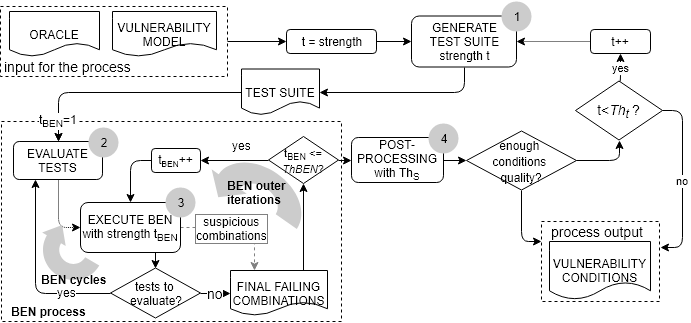
\includegraphics[width=.81\textwidth]{metaprocess.png}
\caption{Condition detection meta-process}\label{fig:metaprocess}
\end{figure}

\bb Fig. \ref{fig:metaprocess} shows an overview of our process to automatically evolve an abstract attack model initialized without constraints, to detect conditions that trigger XSS vulnerabilities.
The process proceeds according to the following steps:

\begin{inparaenum}

\item From a defined initial interaction strength $t$,  derive a  $t$-way test suite.

\item  Mark the test cases as failing or passing according to the current model and the evaluator. 
If all the tests pass and $Th_t$ is not yet reached, increment the strength $t \gets t+1$, and go to point 1. 
Otherwise, evaluate the tests.
Internally, the evaluator executes the translation function $\tau$ to obtain the concrete test string to insert in the \textit{reflection} URL to query the SUT. PhantomJS\footnote{PhantomJS (http://phantomjs.org/) is a headless browser environment enabling introspection of events such as network requests, document edits and JavaScript errors.} then analyzes the HTML code returned by the SUT for a specific \textit{target function} (the \texttt{alert()} function in our case\footnote{in theory, any valid JavaScript functions that will not be called during the normal operation of the SUT can be chosen instead.}) that was included as payload. 
If any of the target functions were executed, the injection was successful; if the page loads normally and does not produce any errors, the injection is deemed unsuccessful.
Lastly, if JavaScript errors are observed on the page, it is likely that some content was injected, but not in a form that constitutes a usable injection (thus resulting in incorrect syntax).
Our current approach regards these test cases as failing, but future evolutionary approaches might take advantage of this particular classification.

\item Pass the evaluated test suite to BEN~\cite{ghandehari2018combinatorial} to derive suspicious combinations, together with their \textit{suspiciousness} level.
We call BEN multiple times specifying the size $t_{BEN}$ of the suspicious combinations to detect\footnote{note that $t_{BEN}$ is different from the strength $t$ for generating the initial test suite}, from 1 to $Th_{BEN}$.
BEN may also ask for a few additional tests (up to 10 tests at a time: \emph{inner BEN cycles}) to reduce the amount of suspicious combinations and improve the accuracy of the computed \emph{suspiciousness} levels.

\item The suspicious combinations from BEN are then translated into a set of constraints for the current knowledge base $K_i$, by negating the corresponding boolean expression (obtained by putting the assignments in conjunction) of every combination whose \textit{suspiciousness} value is above the threshold $Th_S$.  

Due to low accuracy in the detected suspicious combinations, 
we noticed that $K_i$ often results to be a contradiction, which is normally not the case in real-world systems.%, but due to low accuracy. %, but due to low accuracy. 
Therefore, we \textit{post-process} the constraints by computing the \textit{unsat-cores} of $K_i$ and removing all such clauses starting from the \textit{least-suspicious} constraints (according to BEN), until
% the contradiction is solved.
$K_i$ is not a contradiction any longer.
The process eventually quits if either the user is \textit{satisfied} with the quality of $K_i$\footnote{in this case, we believe that the suspiciousness average and standard deviation could be useful indicators of the $F_1$ score that the currently inferred model may have}, or the threshold $Th_t$ is reached.
Otherwise, increase $t$ and go to point 1.
\end{inparaenum}
\be

\subsection{Experiments}\label{sec:xssexperiments}

\bb The process has been implemented in Java using {\tt CTWedge}~\cite{IWCTGargantini2018} to represent and update attack models, {\tt ACTS}~\cite{ACTS} to generate combinatorial test suites of a defined strength, and {\tt BEN}~\cite{ghandehari2018combinatorial} as a tool to detect suspicious combinations and compute suspiciousness.
Experiments were executed on a PC with Intel i7 3.40GHz processor and 16 GB RAM.
We run the process on six real web-applications: four are part of the WAVSEP\footnote{WAVSEP: Web Application Vulnerability Scanner Evaluation Project, \url{https://github.com/sectooladdict/wavsep}.} project, and two are open source content management systems: MiniCMS and NavigateCMS.
Each SUT receives over HTTP one GET parameter which is rejected on the page in different contexts, and might optionally be altered by a specific sanitization function.
Tab. \ref{table:tab1} shows, for each SUT, the respective \textit{vulnerability ratio}, i.e., the ratio of tests that triggered an XSS vulnerability ($\mathit{eval}(f)$) out of the total number of tests executed, that, given the practical infeasibility of the exhaustive test suite, we compute on all the tests generated up to strength t=5 %(one more than the maximum size used in the process, which is 4), consisting of 42830 tests
(42830 tests).\footnote{The tests suites were generated using the IpoF algorithm, implemented in ACTS}\be
\begin{table}[ht]
\centering
\caption{XSS reflection sites on WAVSEP benchmarks}\label{table:tab1}
\resizebox{.9\columnwidth}{!}{%
	\setlength\tabcolsep{1pt}
	\begin{tabular}{c c c c c}
		\toprule
		\shortstack{SUT\\ID} & SUT name & Reflection site
		& \shortstack{vulnerability\\ratio (t=5)} \\
		\midrule
		1 & \footnotesize Tag2HtmlPageScope & {\footnotesize \textsf <body>\$input</body>} & 17.08 \%\\ %& 16.96 \%
		2 & {\footnotesize Tag2TagStructure} & {\footnotesize \textsf <input type="text" value="\$input">} & 4.06 \% \\ %  & 4.05 \%
		3 & \footnotesize Event2TagScope & {\footnotesize\textsf <img src="\$input">} & 4.63 \% \\ %  & 4.58 \%
		4 & \footnotesize Event2DoubleQuotePropertyScope & {\footnotesize \textsf <img src="\$input">} & 3.45 \% \\ %  & 3.27 \%
		5 & \footnotesize MiniCMS & {\footnotesize \textsf /mc-admin/page.php?date=\$input} & 80.2 \% \\
		6 & \footnotesize NavigateCMS & {\footnotesize \textsf /navigate.php?fid=\$input} & 60.0 \% \\		
		\bottomrule
	\end{tabular}%
}
\end{table}

\bb To assess the quality of the evolved knowledge base from our method, we use the typical metrics of information retrieval: in particular, \textit{precision} ($\frac{TP}{TP+FP}$), and \textit{recall} ($\frac{TP}{TP+FN}$) give a measure of how the process isolates true positives, $accuracy$ gives an overall ratio of correctly classified tests, and the $F_1$ score is considered to be a good candidate synthesis index of the inferred model's quality. 
For the experiments, we set the parameters of the process as follows:
\begin{compactitem}
\item $Th_{BEN}=3$. We limited the size of detected suspicious combinations as the BEN process becomes too slow when computing suspiciousness of the too many combinations of size 4 (or larger) on these attack models.
\item $t$, the initial strength of test suite, is set to 2.
\item $Th_t=4$. We limit the maximum strength of the initial test suite since even $t$=5 (about 36000 tests) would make the BEN process too slow.% in computing suspicious combinations.
\item $Th_S=0$, as %in the standard setting 
we want all the suspicious combinations to be considered. %However, in RQ2 we assess quality of the inferred model against variations of this threshold.
\end{compactitem}\be

\begin{table*}[!hbt]
\setlength\tabcolsep{2.5pt}
\centering
\caption{Quality metrics for the inferred models ($Th_{BEN}=3$, and $Th_S=0$)}\label{tab:results}
\resizebox{\textwidth}{!}{%
	\begin{tabular}{rccccccccc}
		\hline
		&   sut & \shortstack{time\\(s)} & constraints & \shortstack{suspiciousness\\avg. $\pm$ s.d.} & accuracy & precision & \shortstack{recall\\(TPR)} & \shortstack{specificity\\(TNR)} &  $F_1$ score \\
		\toprule
		\multirow{7}*{\rotatebox{90}{$Th_t$=4}} & 1 & 246 & 146 & 0.254 $\pm$ 0.0288 & 72.6 & 32.5 & 55.7 & 76.1 &  41.0 \\
		& 2 & 141 & 38 & 0.362 $\pm$ 0.00753 & 93.3 & 32.6 & 59.5 & 94.8 & 42.1 \\
		& 3 & 1437 & 794 & 0.137 $\pm$ 0.0456 & 87.4 & 15.7 & 39.7 & 89.7 & 22.5 \\
		& 4 & 1088 & 551 & 0.136 $\pm$ 0.0483 &   89.0 & 13.7 & 42.3 & 90.6 & 20.7 \\
		& 5 & 1445 & 623 & 0.342 $\pm$ 0.0287 & 78.3 &   87.0 & 85.8 & 48.3 & 86.4 \\
		& 6 & 679 & 80 & 0.344 $\pm$ 0.0147 &   52.0 & 66.6 &   40.0 &   70.0 &   50.0 \\\cline{2-10}
		& avg & 839 & 372 & 0.263 $\pm$ 0.0289 & 78.8 & 41.4 & 53.8 & 78.3 & 43.8 \\
		\midrule%\midrule
		
		\multirow{7}*{\rotatebox{90}{$Th_t$=3}} & 1 & 9.3 & 644 & 0.196  $\pm$ 0.0423 & 41.4 & 19.8 & 79.8 &  33.5 & 31.8 \\
		& 2 & 4.2 &  164 & 0.224  $\pm$ 0.0874 & 78.9 & 14.2 &   83 &  78.7 & 24.2 \\
		& 3 & 28.5 &  764 & 0.207  $\pm$ 0.0628 & 75.4 & 12.9 & 75.7 &  75.3 &   22 \\
		& 4 & 9.3 &  123 & 0.125  $\pm$ 0.0379 & 72.3 & 8.53 & 73.7 &  72.2 & 15.3 \\
		& 5 & 58.5 & 1340 & 0.318  $\pm$ 0.0268 & 80.1 & 80.2 & 99.9 & 0.306 &   89 \\
		& 6 & 37.6 & 2460 & 0.296  $\pm$ 0.0245 & 62.2 & 61.8 & 97.1 &  9.91 & 75.5 \\\cline{2-10}
		& avg & 24.6 & 915 & 0.228 $\pm$ 0.0470 & 68.4 & 32.9 & 84.9 & 45.0 & 43.0 \\
		\bottomrule
	\end{tabular}
}
\end{table*}

\bb Test suites for interaction strengths $t \in \lbrace 3,4\rbrace$ had $900$ and $7200$ test cases, respectively.
For each SUT, Tab. \ref{tab:results} reports the number of constraints included in the inferred model, the average suspiciousness with its standard deviation,
and the accuracy, precision, recall, specificity, and $F_1$ score of the final model, computed over all tests up to strength 5, as for the \textit{vulnerability ratio} in Tab. \ref{table:tab1}.

\researchquestion{What is the quality of the model obtained by the approach?}
We observe that the inferred model achieves an average accuracy of 78.8\%, with a maximum of 93.3\%. Precision has an average of 41.4\%, ranging from 13.7\% to 87\%, and
recall (54\% on average) %, ranging between 40\% and 86\%) 
is higher than precision. %, and specificity is high (78\% on average); 
$F_1$ score is on average 43.8\%, with a maximum of 86.4\% on SUT5.
With relatively few tests ($t$=4 out of 7 parameters), the final model is of good quality, but not completely accurate.
We can also observe that $F_1$ is proportional to the vulnerability ratio of the SUT.

\researchquestion{How does the quality of the inferred model vary depending on $Th_t$?}
By increasing $Th_t$ from 3 to 4, the time taken, as expected, increases, while the number of constraints, in most cases, decreases, meaning that with more tests our process is able to describe the vulnerability conditions with fewer constraints.
On average, although recall decreases, both precision, accuracy and specificity increase, %significantly,
and $F_1$ slightly increases. This means that the classification %of true vulnerability-triggering or non-triggering tests
improves.%, and in particular more tests that do not trigger any actual vulnerability are found.

\researchquestion{Which is the computational effort of the proposed process?}
%We are here interested in the effort required by the proposed approach in terms of computation time.
Tab.~\ref{tab:results} also reports the total execution time, excluding the actual test execution, as test results are cached, except for the few tests (30 at most) that BEN may ask during the process.
For the first two SUTs, the process takes less than 250 seconds to complete, but up to 24 minutes are needed for SUT5 with $Th_t=4$. 
Most of the computation time is used internally by BEN; by limiting to 3 the strength of the initial test suite, the total time is always below 1 minute for every SUT. %For the other SUTs and for the normal approach, the process takes from about 15 to about 30 minutes to complete.

\researchquestion{How does variations of $Th_S$ affect model quality?}
The highest $F_1$ score is achieved with low values of $Th_S$ (see Fig. \ref{fig:f1ByThs}), except for SUT3 and SUT4, for which a $\overline{Th_S} \simeq 0.13$ achieves the maximum $F_1$ score. However, we can notice that at least around 25\% of the constraints (starting from the least suspicious ones) can be removed with negligible impact on the final $F_1$ score.\be
\begin{figure*}[!hbt]
\centering
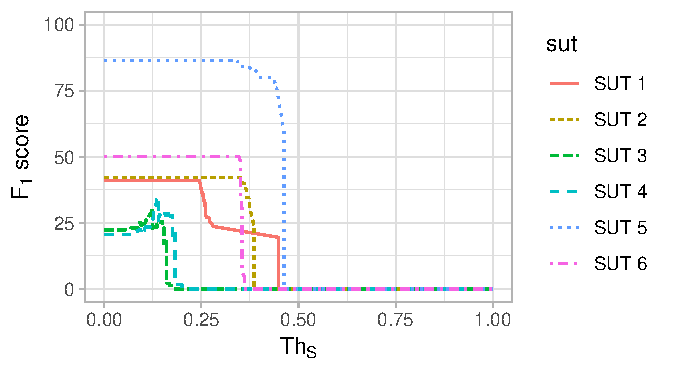
\includegraphics[width=.49\textwidth]{SUT_4.pdf}
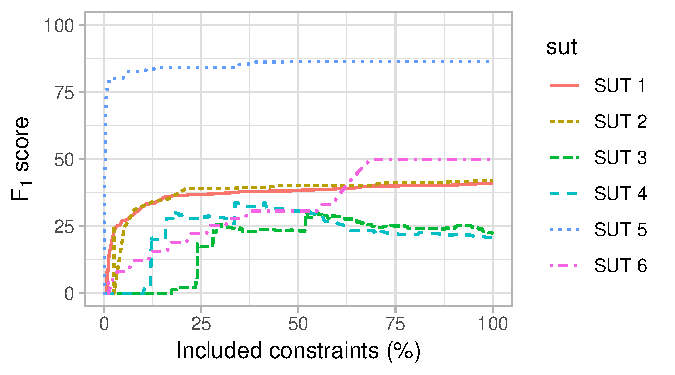
\includegraphics[width=.49\textwidth]{SUT_4_percConstr.pdf}
\caption{Achieved $F_1$ score of final model by varying $Th_S$, when $Th_t=4$
}\label{fig:f1ByThs}
\end{figure*}

\subsection{Related Work}\label{sec:xssrelatedwork}
\bb XSS vulnerability detection is not a novel topic in computer science research. %;  many works tried to propose different techniques to address this problem.
Duchene et al.~\cite{Duchene:2012} used model based testing and fuzzing to discover XSS vulnerabilities; Melicher et al.~\cite{melicher_riding_2018} proposed improvements on using the DOM model to generate
and detect
XSS attacks; %, and discusses possible countermeasures to prevent XSS vulnerabilities; %\todo{this came from the reviewer}
Simos et al.~\cite{wotawa_combinatorial_2016} proposed a combinatorial approach to find attack vectors that trigger XSS vulnerabilities; Jia et al.~\cite{Jia:2015} %and Temple et al.~\cite{temple_using_2016}
used machine learning and hyper-heuristic search to improve combinatorial tests% and infer constraints among parameters.
; Temple et al.~\cite{Temple16:using} proposed a machine-learning approach to infer constraints among parameters that, although not sound, achieves high precision (about 90\%) and recall (80\%).
Although these works use model-based testing,%  or fuzzing,
the usage of combinatorial testing for XSS vulnerability detection to \textit{classify} vulnerabilities based on the input and describe \textit{completely} the vulnerability space of a part of a web application, evolving a \textit{knowledge base}, is the main novelty of our approach.
The first phase of BEN~\cite{ghandehari2018combinatorial} as a failure-inducing combination detection and ranking tool 
has been used by Gargantini et al.~\cite{gargantini_combinatorial_2017} to repair constraints in combinatorial models, evaluating different test generation policies.
\be

\section{Conclusion and Future Work}\label{sec:conclusion-future-work}

In this chapter, we presented an approach that extends CIT and aims to (1) automatically check the validity of the configurability model of the system under test, (2) automatically finding and fixing faults in models of parameter configurations of software systems, and (3) evolve an attack model to include conditions among input parameters that trigger XSS vulnerabilities in web applications. 

For checking the validity of the combinatorial model, we devised four original policies that can help software testers discover faults in the model of system configurations as well as faults in the software implementation that the model describes \cite{Gargantini16:validation} Several experiments conducted show the efficacy of our approach.   We confirm that constraints play an important role in configurability testing, but the experiments show that also invalid configurations should be considered in order to avoid some problems (like over-specification) and to detect a wider range of faults. 
Our experiments suggest that techniques including both valid and invalid tests (as \cucv) have a better fault detection capability than techniques including only valid (as \ccit) or invalid tests (as \cv). However, producing invalid tests may be not feasible. In these cases we would suggest the tester to use \CCi instead of \ic and \ccit. The experiments suggest that \CCi is not very expensive and it offers a superior fault detection capability. The techniques presented should significantly help software developers in the modeling and testing process of software systems configurations.

We then used these novel CIT policies in an iterative process for finding and fixing conformance faults \cite{gargantini_combinatorial_2017}. This process can help software testers discover faults in the model of system configurations as well as faults in the software implementation that the model describes. We call these conformance faults.
We then conduct several experiments on five software systems to validate our approach. We show that we can successfully repair existing combinatorial models. Furthermore, we also show how our approach can be utilised to derive constraints between parameters of large complex software systems. The technique presented should help software developers derive and fix combinatorial testing models by automating this often purely manual and thus time-consuming and highly error-prone task.

As third step, in \cite{garn2019}, we introduce the notion of \textit{suspicious combination}, that allows to apply the iterative process devised in \cite{gargantini_combinatorial_2017} to the detection of XSS vulnerability-triggering conditions among input parameters.
Suspicious combinations are combinations whose appearance in a test vector would trigger a discrepancy between the \textit{best-guess} of the current model, and the actual outcome when executed against the SUT.
Identification of constraints among XSS attack parameters helps to better understand
the root cause of an XSS vulnerability and provides insights about how to fix
a flawed sanitization function.
As future work, we plan to improve the process by reducing the required tests, using information from previous step, and evaluating alternatives to BEN, such as MixTgTe \cite{iwct19}. We believe that this approach can be extended to other security vulnerabilities related to sanitization functions, and to detect discrepancies between a functional system specification and its implementation.
Another direction is to further simplify the detected constraints, to reduce them in number and present them to the user in a more readable way, applying methods such as the ones in \cite{arcaini2019varivolution}.

%We propose a novel approach for automatically finding and fixing faults in models of parameter configurations of software systems. 
%In particular, we described how combinatorial testing techniques can be utilised for this purpose. 






\chapter{Repair of Timed Automata}\label{ch:tarepair}
%\begin{tikzborder}{\cite{andre_tap_2019}}
Timed automata (TAs) \cite{AD94} are a widely used formalism to specify systems having temporal requirements. However, exactly specifying the system may be difficult, as the user may not know the exact clock constraints triggering state transitions. In this work, we assume the user already specified a \ta, and (s)he wants to validate it against an oracle that can be queried for acceptance. Under the assumption that the user only wrote wrong guard transitions (\ie{} the structure of the TA is correct), the search space for the correct TA can be represented by a Parametric Timed Automaton (PTA), \ie{} a TA in which some constants are parametrized.
This chapter presents the content of the paper \cite{andre_tap_2019}, that introduces a process that
%
\begin{inparaenum}[(i)]
	\item abstracts the initial (faulty) TA \initTa in a PTA \ptaProc;
	\item generates some test data (\ie{} timed traces) from \ptaProc;
	\item assesses the correct evaluation of the traces with the oracle;
	\item uses the \imitator tool for synthesizing some constraints \ptaConstr on the parameters of \ptaProc;
	\item instantiate from \ptaConstr a \ta \repTa as final repaired model.
\end{inparaenum}
%
Experiments show that the approach is successfully able to partially repair the initial design of the user.
%\end{tikzborder}

%\section{Introduction}

%\begin{tikzborder}{}	
%Timed automata (\ta)~\cite{AD94} represent a widely used formalism for modeling and verifying concurrent timed systems.
A common usage of timed automata
 is to develop a \ta describing the running system and then apply analysis techniques to it (\eg{} \cite{BY03}). However, exactly specifying the system under analysis may be difficult, as the user may not know the exact clock constraints that trigger state transitions, or may perform errors at design time. Therefore, validating the produced \ta against the real system is extremely important to be sure that we are analyzing a faithful representation of the system. Different testing techniques have been proposed for timed automata, based on different coverage criteria as, \eg{} transition coverage~\cite{springintveld2001testing} and fault-based coverage~\cite{Aichernig2015MMT,aichernig2013time}, and they can be used for \ta validation. However, once some failing tests have been identified, it remains the problem of detecting and removing ({\it repair}) the fault from the \ta under validation. How to do this in an automatic way is challenging. One possible solution could be to use mutation-based approaches~\cite{Aichernig2015MMT,aichernig2013time} in which mutants are considered as possible repaired versions of the original \ta; however, due to the continuous nature of timed automata, the number of possible mutants (\ie{} repair actions) is too big also for small \tas and, therefore, such approaches do not appear to be feasible. We here propose to use a {\it symbolic representation} of the possible repaired \tas and we reduce the problem of repairing to finding an assignment of this symbolic representation.

\fakeparagraph{Contribution}
In this work, we address the problem of testing/validating \tas under the assumption that only clock guards may be wrong, that is, we assume that the structure (states and transitions) is correct.
Moreover, we assume to have an oracle that we can query for acceptance of timed traces, but whose internal structure is unknown: this oracle can be a Web-service, a medical device, a protocol, etc. In order to symbolically represent the search space of possible repaired \tas, we use the formalism of parametric timed automata (PTAs)~\cite{AHV93} as an abstraction to represent all possible behaviors under all possible clock guards.

We propose a framework for automatic repair of \tas that takes as input a \ta \initTa to repair and an {\it oracle}. The process works as follows:
%
\begin{ienumeration}
	\item starting from \initTa, we build a PTA \ptaProc where to look for the repaired \ta;
	\item we build a symbolic representation of the language accepted by \ptaProc in terms of an {\it extended parametric zone graph} \epzg;
	\item we then generate some test data \testData from \epzg;
	\item we assess the correct evaluation of \testData by querying the {\it oracle}, so building the test suite \testSuiteTA;
	\item we feed the tests \testSuiteTA to the \imitator tool that finds some constraints \ptaConstr that restrict \ptaProc only to those \tas that correctly evaluate all the tests in \testSuiteTA;
	\item as the number of \tas that are correct repairs may be infinite, we try to obtain, using a constraint solver based on local search, the \ta \repTa closest to the initial \ta \initTa. Note that trying to modify as less as possible the initial \ta is reasonable if we assume the competent programmer hypothesis~\cite{surveyMutationTestingPapadakis2018}.
\end{ienumeration}

To evaluate the feasibility of the approach, we performed some preliminary experiments showing that the approach is able to (partially) repair a faulty \ta. 

\fakeparagraph{Outline}
\ref{sec:definitions1} explains the definitions we need in our approach.
Then \ref{sec:proposedApproachSingle} presents the process we propose that combines model abstraction, test generation, constraint generation, and constraint solving.
\ref{sec:evaluation2} describes experiments we performed to evaluate our process.
Finally, \ref{sec:related1} reviews some related work, and \ref{sec:conclusions2} concludes the paper.
%\end{tikzborder}

\section{Definitions}\label{sec:definitions1}

\begin{tikzborder}{}
A \emph{timed word}~\cite{AD94} over an alphabet of actions~$\Actions$ is a possibly infinite sequence of the form
$(\action_0 , d_0) (\action_1, d_1) \cdots$
such that, for all integer $i \geq 0$, $\action_i \in \Actions$ and $d_i \leq d_{i+1}$.
A timed language is a (possibly infinite) set of timed words.

We assume a set~$\Clock = \{ \clock_1, \dots, \clock_\ClockCard \} $ of \emph{clocks}, \ie{} real-valued variables that evolve at the same rate.
A clock valuation is 
$\clockval : \Clock \rightarrow \Rgeqzero$.
We write $\ClocksZero$ for the clock valuation assigning $0$ to all clocks.
Given $d \in \Rgeqzero$, $\clockval + d$ is \st{} $(\clockval + d)(\clock) = \clockval(\clock) + d$, for all $\clock \in \Clock$.
%
Given $\resets \subseteq \Clock$, we define the \emph{reset} of a valuation~$\clockval$, denoted by $\reset{\clockval}{\resets}$, as follows: $\reset{\clockval}{\resets}(\clock) = 0$ if $\clock \in \resets$, and $\reset{\clockval}{\resets}(\clock)=\clockval(\clock)$ otherwise.

We assume a set~$\Param = \{ \param_1, \dots, \param_\ParamCard \} $ of \emph{parameters}.
A parameter {\em valuation} $\pval$ is
$\pval : \Param \rightarrow \grandqplus$.
We assume ${\compOp} \in \{<, \leq, =, \geq, >\}$.
A \emph{clock guard}~$\guard$ is a constraint over $\Clock \cup \Param$ defined by a conjunction of inequalities of the form
$\clock \compOp \sum_{1 \leq i \leq \ParamCard} \alpha_i \param_i + d$, with
$\param_i \in \Param$,
and
$\alpha_i, d \in \grandz$.
%
Given~$\guard$, we write~$\clockval\models\pval(\guard)$ if %$\valuate{\valuate{\guard}{\pval}}{\clockval}$
the expression obtained by replacing each~$\clock$ with~$\clockval(\clock)$ and each~$\param$ with~$\pval(\param)$ in~$\guard$ evaluates to true.
\end{tikzborder}

\subsection{Parametric timed automata}

\begin{tikzborder}{}	
\begin{definition}[PTA]\label{def:uPTA}
	A PTA $\A$ is a tuple \mbox{$\A = (\Actions, \Loc, \locinit, \LocsFinal, \Clock, \Param, \invariant, \Edges)$}, where:
	\begin{ienumeration}
		\item $\Actions$ is a finite set of actions,
		\item $\Loc$ is a finite set of locations,
		\item $\locinit \in \Loc$ is the initial location,
		\item $\LocsFinal \subseteq \Loc$ is the set of accepting locations,
		\item $\Clock$ is a finite set of clocks,
		\item $\Param$ is a finite set of parameters,
		\item $\invariant$ is the invariant, assigning to every $\loc\in \Loc$ a clock guard $\invariant(\loc)$,
		\item $\Edges$ is a finite set of edges $\edge = (\loc,\guard,\action,\resets,\loc')$
		where~$\loc,\loc'\in \Loc$ are the source and target locations, $\action \in \Actions$, $\resets\subseteq \Clock$ is a set of clocks to be reset, and $\guard$ is a clock guard.
	\end{ienumeration}
\end{definition}

Given $\edge = (\loc,\guard,\action,\resets,\loc')$, we define $\act(\edge) = \action$.

\begin{example}
	Consider the PTA in \ref{figure:example-PTA}, containing two clocks~$\styleclock{x}$ and \styleclock{y} and three parameters~$\parami{2}$, $\parami{3}$ and~$\parami{4}$.
	The initial location is~$\loc_1$.
\end{example}
\end{tikzborder}

\begin{figure}[!htb]
	\begin{subfigure}[b]{0.49\textwidth}
		\centering
		\footnotesize
		
		\begin{tikzpicture}[scale=1, xscale=1.1, yscale=1.1, auto, ->, >=stealth']
		
		\node[location, initial] at (0, 0) (l1) {$\loc_1$};
		
		\node[location] at (2, 0) (l2) {$\loc_2$};
		
		\node[location] at (4, 0) (l3) {$\loc_3$};
		
		\node[location] at (2, -1) (l4) {$\loc_4$};
		
		\node[location] at (4, -1) (l5) {$\loc_5$};
		
		\node[invariant, above=of l1] {$\styleclock{\clock} \leq 4$};
		\node[invariant, below=of l2] {$\styleclock{\clock} \leq 3$};
		\node[invariant, below=of l4] {$\styleclock{\clock} \leq 6$};
		
		\path (l1) edge node[align=center]{$\styleclock{\clock} \leq 3$} node[below]{$\styleact{a}$} (l2);
		\path (l2) edge node[align=center]{$\styleclock{\clock} = 3 \land \styleclock{y} \geq 4$} node[below]{$\styleact{b}$} (l3);
		\path (l1) edge[bend right] node[left, align=center]{$\styleclock{\clock} > 2$ \\ $\styleact{a}$ \\ $\styleclock{y} := 0$} (l4);
		\path (l4) edge node[align=center]{$\styleclock{y} > 1 \land \styleclock{x} > 4$} node[below]{$\styleact{c}$} (l5);
		
		\end{tikzpicture}
		\caption{A TA to be repaired}
		\label{figure:example-TA}
		
	\end{subfigure}
	\hfill
	\begin{subfigure}[b]{0.49\textwidth}
		\centering
		\footnotesize
		
		\begin{tikzpicture}[scale=1, xscale=1.1, yscale=1.1, auto, ->, >=stealth']
		
		\node[location, initial] at (0, 0) (l1) {$\loc_1$};
		
		\node[location] at (2, 0) (l2) {$\loc_2$};
		
		\node[location] at (4, 0) (l3) {$\loc_3$};
		
		\node[location] at (2, -1) (l4) {$\loc_4$};
		
		\node[location] at (4, -1) (l5) {$\loc_5$};
		
		\node[invariant, above=of l1] {$\styleclock{\clock} \leq 4$};
		\node[invariant, below=of l2] {$\styleclock{\clock} \leq \parami{3}$};
		\node[invariant, below=of l4] {$\styleclock{\clock} \leq 6$};
		
		\path (l1) edge node[align=center]{$\styleclock{\clock} \leq \parami{3}$} node[below]{$\styleact{a}$} (l2);
		\path (l2) edge node[align=center]{$\styleclock{\clock} = \parami{3} \land \styleclock{y} \geq 4$} node[below]{$\styleact{b}$} (l3);
		\path (l1) edge[bend right] node[left, align=center]{$\styleclock{\clock} > \parami{2}$ \\ $\styleact{a}$ \\ $\styleclock{y} := 0$} (l4);
		\path (l4) edge node[align=center]{$\styleclock{y} > 1 \land \styleclock{x} > \parami{4}$} node[below]{$\styleact{c}$} (l5);
		
		\end{tikzpicture}
		\caption{An abstract PTA}
		\label{figure:example-PTA}
		
	\end{subfigure}
	\caption{Running example}
	\label{figure:example}
\end{figure}
%----------------------------------------------------------

\begin{tikzborder}{}
Given~$\pval$, we denote by $\valuate{\A}{\pval}$ the non-parametric structure where all occurrences of a parameter~$\param_i$ have been replaced by~$\pval(\param_i)$.

We denote as a \emph{timed automaton} any such structure $\valuate{\A}{\pval}$.

The \emph{synchronous product} (using strong broadcast, \ie{} synchronization on a given set of actions), or \emph{parallel composition}, of several PTAs gives a PTA (see \ref{appendix:parallel} for a common formal definition).

%----------------------------------------------------------
\begin{definition}[Concrete semantics of a TA]
	Given a PTA $\A = (\Actions,$ $\Loc,$ $\locinit,$ $\LocsFinal,$ $\Clock,$ $\Param,$ $\invariant,$ $\Edges)$,
	and a parameter valuation~\(\pval\),
	the semantics of $\valuate{\A}{\pval}$ is given by the timed transition system (TTS) $(\States, \sinit, \flecheRel)$, with
	\begin{compactitem}
		\item $\States = \{ (\loc, \clockval) \in \Loc \times \Rgeqzero^\ClockCard \mid \clockval \models \valuate{\invariant(\loc)}{\pval} \}$, % \valuate{\valuate{\invariant(\loc)}{\pval}}{\clockval} \text{ evaluates to true}
		 $\sinit = (\locinit, \ClocksZero) $,
		\item $\flecheRel$ consists of the discrete and (continuous) delay transition relations:
		\begin{ienumeration}
			\item discrete transitions: $(\loc,\clockval) \longueflecheRel{\edge} (\loc',\clockval')$, %with $\action \in \Sigma$,
			if $(\loc, \clockval) , (\loc',\clockval') \in \States$, and there exists $\edge = (\loc,\guard,\action,\resets,\loc') \in \Edges$, such that $\clockval'= \reset{\clockval}{\resets}$, and $\clockval\models\pval(\guard$).
			% $\valuate{\valuate{\guard}{\pval}}{\clockval}$ evaluates to true.
			\item delay transitions: $(\loc,\clockval) \longueflecheRel{d} (\loc, \clockval+d)$, with $d \in \Rgeqzero$, if $\forall d' \in [0, d], (\loc, \clockval+d') \in \States$.
		\end{ienumeration}
	\end{compactitem}
\end{definition}

Moreover we write $(\loc, \clockval)\longuefleche{(\edge, d)} (\loc',\clockval')$ for a combination of a delay and discrete transition if
% d,
$\exists \clockval'' : (\loc,\clockval) \longueflecheRel{d} (\loc,\clockval'') \longueflecheRel{\edge} (\loc',\clockval')$.

Given a TA~$\valuate{\A}{\pval}$ with concrete semantics $(\States, \sinit, \flecheRel)$, we refer to the states of~$\States$ as the \emph{concrete states} of~$\valuate{\A}{\pval}$.
A \emph{run} of~$\valuate{\A}{\pval}$ is an %possibly infinite
alternating sequence of concrete states of $\valuate{\A}{\pval}$ and pairs of edges and delays starting from the initial state $\sinit$ of the form
$\state_0, (\edge_0, d_0), \state_1, \cdots$
with
$i = 0, 1, \dots$, $\edge_i \in \Edges$, $d_i \in \Rgeqzero$ and
$\state_i \longuefleche{(\edge_i, d_i)} \state_{i+1}$.
The \emph{associated timed word} is $(\act(\edge_0) , d_0) (\act(\edge_1), \sum_{0 \leq i \leq 1} d_i) \cdots$.
A run is \emph{maximal} if it is infinite or cannot be extended by any discrete action.
The (timed) language of a TA, denoted by $\Lg(\valuate{\A}{\pval})$, is the set of timed words associated with maximal runs of~$\valuate{\A}{\pval}$.
Given~$\state=(\loc, \clockval)$, we say that $\state$ is reachable in~$\valuate{\A}{\pval}$ if $\state$ appears in a run of $\valuate{\A}{\pval}$.
By extension, we say that $\loc$ is reachable in~$\valuate{\A}{\pval}$; and by extension again, given a set~$\somelocs$ of locations, we say that $\somelocs$ is reachable if there exists $\loc \in \somelocs$ such that $\loc$ is reachable in~$\valuate{\A}{\pval}$.


%----------------------------------------------------------
\begin{example}
	Consider the TA~$\A$ in \ref{figure:example-TA}.
	Consider the following run~$\varrun$ of $\A$:
	\[
	\Big(\loc_1,
	\left ( \begin{array}{l}
	\styleclock{x} = 0 \\
	\styleclock{y} = 0 \\
	\end{array}
	\right ) \Big)
	,
	(\styleact{a}, 2.5)
	,
	\Big(\loc_4,
	\left ( \begin{array}{l}
	\styleclock{x} = 2.5 \\
	\styleclock{y} = 0 \\
	\end{array}
	\right ) \Big)
	,
	(\styleact{c}, 2)
	,
	\Big(\loc_5,
	\left ( \begin{array}{l}
	\styleclock{x} = 4.5 \\
	\styleclock{y} = 2 \\
	\end{array}
	\right ) \Big)
	\]
	
	We write ``$\styleclock{\clock} = 2.5$'' instead of ``$\clockval$ such that $\clockval(\styleclock{\clock}) = 2.5$''.
	The associated timed word is $(\styleact{a}, 2.5) (\styleact{c}, 4.5)$.
\end{example}
\end{tikzborder}

\subsection{Reachability synthesis}

\begin{tikzborder}{}
We will use reachability synthesis to solve the problem in \ref{ss:problem}.
This procedure, called \EFsynth{}, takes as input a PTA~$\A$ and a set of target locations~$\somelocs$, and attempts to synthesize all parameter valuations~$\pval$ for which~$\somelocs$ is reachable in~$\valuate{\A}{\pval}$.
$\EFsynth(\A, \somelocs)$ was formalized in \eg{} \cite{JLR15} and is a procedure that traverses the parametric zone graph of~$\A$;
\EFsynth{} may not terminate (because of the infinite nature of the graph), but computes an exact result (sound and complete) if it terminates.


%----------------------------------------------------------
\begin{example}
	Consider again the PTA~$\A$ in \ref{figure:example-PTA}.
	% 	 p4 >= 0
	% & p2 >= 0
	% & 6 > p4
	% & 4 > p2
	% & p3 >= 0
	$\EFsynth(\A, \{ \loc_5 \})$ returns $0 \leq \parami{2} < 4 \land 0 \leq \parami{4} \leq 6 \land \parami{3} \geq 0$.
	Intuitively, this corresponds to all parameter constraints in the parametric zone graph in \ref{figure:example-PTA:PZG} associated to symbolic states with location~$\loc_5$ (there is a single such state).
\end{example}
\end{tikzborder}

\section{A repairing process using abstraction and testing}\label{sec:proposedApproachSingle}

\begin{tikzborder}{}
In this paper, we address the \emph{guard-repair} problem of timed automata.
Given a reference TA~$\initTa$ and an oracle~$\oracleTa$ knowing an unknown timed language~$\TLoracle$, our goal is to modify (``repair'') the timing constants in the clock guards of~$\A$ such that the repaired automaton matches the timed language~$\TLoracle$.
%
The setting assumes that the oracle \oracleTa can be queried for acceptance of timed words by~$\TLoracle$; that is, $\oracleTa$ can decide whether a timed word belongs to~$\TLoracle$, but the internal structure of the object leading to~$\TLoracle$ (\eg{} an unknown timed automaton) is unknown.
%
This setting makes practical sense when testing black-box systems.

\defProblem
{guard-repair}
{an initial TA~$\initTa$, an unknown timed language~$\TLoracle$}
{Repair the constants in the clock guards of~$\initTa$ so as to obtain a TA~$\repTa$ such that $\Lg(\repTa) = \TLoracle$}

While the ultimate goal is to solve this problem, in practice the best we can hope for is to be \emph{as close as possible} to the unknown oracle TA, notably due to the undecidability of language equivalence of timed automata~\cite{AD94} (\eg{} if~$\TLoracle$ was generated by another TA).
\end{tikzborder}

\subsection{Overview of the method}

\begin{tikzborder}{}
From now on, we describe the process we propose to automatically repair an initial timed automaton \initTa.
\ref{fig:repairProcess} describes the approach:
\end{tikzborder}
\begin{figure}[!htb]
	\centering
	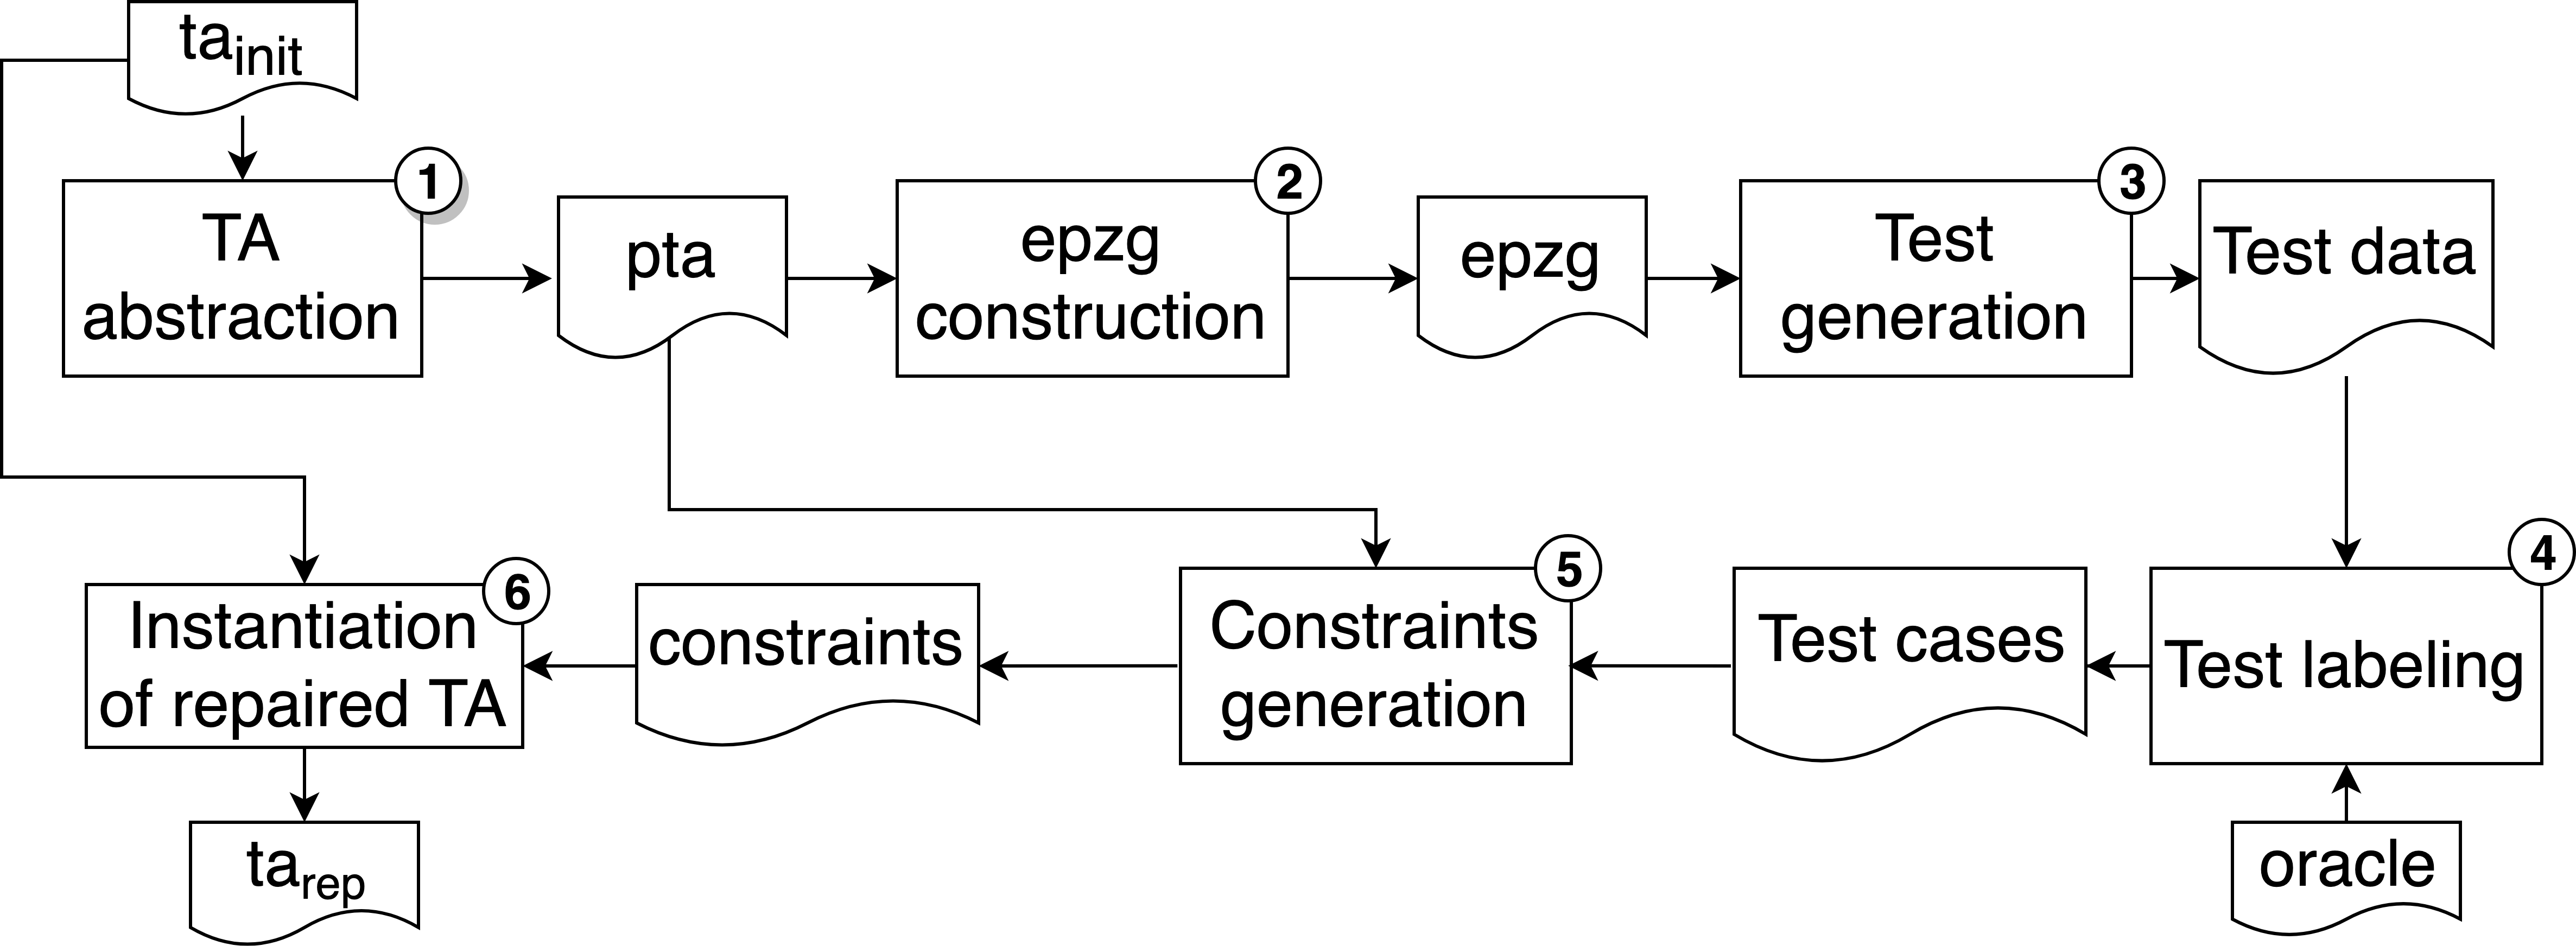
\includegraphics[width=0.8\textwidth]{images/repairProcess-oneShot}
	\caption{Automatic repair process}
	\label{fig:repairProcess}
\end{figure}
%
\begin{description}
	\item[Step \ding{192}] a PTA \ptaProc is generated starting from the initial \ta \initTa.
	\item[Step \ding{193}] the extended parametric zone graph \epzg (an extension of $\PZG$) is built.
	\item[Step \ding{194}] a test generation algorithm generates relevant test data \testData from \epzg.
	%By analyzing \ptaProc and possibly also \initTa, test sequences are produced (\ref{line:genTestsSingle} in \ref{alg:proposedApproachSingle}).
	\item[Step \ding{195}] \testData is evaluated using the oracle, therefore building the test suite \testSuiteTA.
	\item[Step \ding{196}] some constraints \ptaConstr are generated, restricting \ptaProc to the \tas that evaluate correctly the generated tests \testSuiteTA.
	\item[Step \ding{197}] one possible \ta satisfying the constraints \ptaConstr is obtained.
\end{description}

\begin{tikzborder}{}
\ref{alg:proposedApproachSingle} formalizes steps \ding{192}--\ding{196} for which we can provide some theoretical guarantees (\ie{} the non-emptiness of the returned valuation set, and its inclusion of~$\TLoracle$).
\end{tikzborder}
\begin{algorithm}[!htb]
	\begin{algorithmic}[1]
	\Require{\initTa: initial timed automaton to repair}
	\Require{\oracleTa: an oracle assessing the correct evaluation of timed words}
	\Ensure{$\ptaConstr$: set of valuations repairing \initTa}
	
	\State{$\ptaProc \gets \abstractInPta(\initTa)$}\label{line:abstractPtaSingle}
	
	\State{$\epzg \gets \buildEpzg(\ptaProc)$}\label{line:buildEpzg}
	
	\State{$\testData \gets \genTestData(\epzg)$} \Comment{Generate test data from \epzg}\label{line:genTestsSingle}
	
	\State{$\testSuiteTA \gets \labelTests(\testData, \oracleTa)$} \Comment{A test is a pair (trace, assessment)}\label{line:assessTestsSingle}
	
	\Return{$\ptaConstr \gets \genConstr(\ptaProc, \testSuiteTA)$}\label{line:genConstrSingle}
\end{algorithmic}
	\caption{Automatic repair process $\ourMethod(\initTa, \oracleTa)$}
	\label{alg:proposedApproachSingle}
\end{algorithm}
%
\begin{algorithm}[!htb]
	\begin{algorithmic}[1]
	\State {$\mba \gets \{\word \mid (\word, \BTrue) \in \testSuiteTA\}$} \Comment{Tests that must be accepted}\label{line:initMbaSingle}
	
	\State {$\mbr \gets \{\word \mid (\word, \BFalse) \in \testSuiteTA\}$} \Comment{Tests that must be rejected}\label{line:initMbrSingle}
	
	\Return{$\bigwedge_{\word \in \mba} \replayTW(\ptaProc, \word) \land \bigwedge_{\word \in \mbr} \neg \replayTW(\ptaProc, \word)$}\label{line:returnPhiSingle}
\end{algorithmic}
	\caption{GenConstraints($\ptaProc, \testSuiteTA$)}
	\label{algo:genConstr}
\end{algorithm}

\begin{tikzborder}{}
For step \ding{197}, instead, different approaches could be adopted: in the paper, we discuss a possible one. We describe each phase in details in the following sections.
\end{tikzborder}

\subsection{Step \ding{192}: Abstraction}\label{sec:abstraction}

\begin{tikzborder}{}
Starting from the initial \initTa, through \emph{abstraction}, the user obtains a PTA \ptaProc that generalizes \initTa in all the parts that can be possibly changed in order to repair \initTa (\ref{line:abstractPtaSingle} in \ref{alg:proposedApproachSingle}). For instance, a clock guard with a constant value can be parametrized. Therefore, \ptaProc represents the set of all the \tas that can be obtained when repairing \initTa. \ptaProc is built on the base of the domain knowledge of the developer who has a guess of the guards that may be faulty. 

\begin{example}
	Consider again the TA in \ref{figure:example-TA}.
	A possible abstraction of this TA is the PTA in \ref{figure:example-PTA}, where we chose to abstract some of the timing constants with parameters.
	Note that not all timing constants must necessarily be substituted with parameters; also note that a same parameter can be used in different places (this is the case of \parami{3}).
\end{example}

\paragraph{Assumption}
We define below an important assumption for our method; we will discuss in \ref{ss:discussion-abstraction} how to lift it.

\begin{assumption}\label{assumption:oracle-in-pta}
	We here assume that \ptaProc is a correct abstraction, \ie{} it contains a \ta that precisely models the {\it oracle}.
	That is, there exists $\pvalOracle$ such that $\Lg(\valuate{\ptaProc}{\pvalOracle}) = \TLoracle$.
\end{assumption}

Note that this assumption is trivially valid if faults lay in the clock guards (which is the setting of this work), and if all constants used in clock guards are turned to parameters.
\end{tikzborder}

\subsection{Step \ding{193}: construction of the extended parametric zone graph}
\begin{tikzborder}{}
Starting from \ptaProc, we build a useful representation of its computations in terms of an {\it extended parametric zone graph} \epzg (\ref{line:buildEpzg} in \ref{alg:proposedApproachSingle}).
This original data structure will be used for test generation.
In the following, we describe how we build \epzg from \PZG.

We extend the parametric zone graph~$\PZG$ with the two following pieces of information:
\begin{description}
	\item[the parameter constraint characterizing each symbolic state:] from a state $(\loc, C)$, the parameter constraint is $\projectP{C}$ and gives the exact set of parameter valuations for which there exists an equivalent concrete run in the automaton. That is, a state $(\loc, C)$ is reachable in $\valuate{\A}{\pval}$ iff $\pval \models C$ (see \cite{JLR15} for details).
	\item[the minimum and maximum arrival times:] that is, we compute the minimum ($m_i$) and maximum ($M_i$) over all possible parameter valuations of the possible absolute times reaching this symbolic state.
\end{description}
While the construction of the first information is standard, the second one is original to our work and requires more explanation.
We build for each state a (possibly unbounded) interval that encodes the absolute minimum and maximum arrival time.
This can be easily obtained from the parametric zone graph by adding an extra clock never reset (that encodes the absolute time), and projecting the obtained constrained on this extra clock, thus giving minimum and maximum times over all possible parameter valuations.

%----------------------------------------------------------
\begin{example}\label{example:structure}
	Consider again the PTA~$\A$ in \ref{figure:example-PTA} and its parametric zone graph in \ref{figure:example-PTA:PZG}. The parameter constraints associated to each of the symbolic states, and the possible absolute reachable times, are given in \ref{table:extended-PZG}.
	
	\begin{table}[!htb]
		\caption{Description of the states of the extended parametric zone graph}
		\centering
		\begin{tabular}{l | l | l}
			\hline
			\rowHeader{} Symbolic states & Parameter constraint & Reachable times \\
			\hline
			$\symbstate_1$ & $\parami{2} \geq 0 \land \param_3 \geq 0 \land \param_4 \geq 0 $ & $\clockabs = 0$ \\
			\hline
			$\symbstate_2$ & $\parami{2} \geq 0 \land \param_3 \geq 0 \land \param_4 \geq 0 $ & $\clockabs \in [0, 4]$ \\
			\hline
			$\symbstate_3$ & $\parami{2} \geq 0 \land \param_3 \geq 4 \land \param_4 \geq 0 $ & $\clockabs \in [4, \infty)$ \\
			\hline
			$\symbstate_4$ & $4 > \parami{2} \geq 0 \land \param_3 \geq 0 \land \param_4 \geq 0 $ & $\clockabs \in (0, 4]$ \\
			\hline
			$\symbstate_5$ & $4 > \parami{2} \geq 0 \land \param_3 \geq 0 \land 6 > \param_4 \geq 0 $ & $\clockabs \in (1, 6]$ \\
			\hline
		\end{tabular}
		\label{table:extended-PZG}
		
	\end{table}
\end{example}
%----------------------------------------------------------


%----------------------------------------------------------
\begin{remark}
	If all locations of the original PTA contain an invariant with at least one inequality of the form $\clock \compOpLeq \param$ or $\clock \compOpLeq d$, with $\compOpLeq \in \{ <, \leq \}$, and if the parameters are bounded, then the maximum arrival time in each symbolic state will always be finite.
	Note that this condition is not fulfilled in \ref{example:structure} because $\loc_2$ features an invariant $\styleclock{x} \leq \parami{3}$, with $\parami{3}$ unbounded, thus allowing to remain arbitrarily long in~$\loc_2$ for an arbitrarily large value of~$\parami{3}$.
	Therefore, the arrival time in~$\loc_3$ is $\clockabs \in [4, \infty)$.
\end{remark}
%----------------------------------------------------------

\end{tikzborder}

\subsection{Step \ding{194}: Test data generation}\label{sec:testDataGen}
\begin{tikzborder}{}
Starting from \epzg, we generate some test data (\ref{line:genTestsSingle} in \ref{alg:proposedApproachSingle}) in terms of timed words.
\end{tikzborder}

\subsubsection{Constructing timed words}
\begin{tikzborder}{}
We use the minimal and maximum arrival times in the abstract PTA to generate test data.
That is, we will notably use the \emph{boundary} information, \ie{} runs close to the fastest and slowest runs, to try to discover the actual timing guards of the oracle.

The procedure to generate a timed word from the EPZG is as follows:
\begin{compactenum}
	\item Pick a run $\symbstate_0 \edge_0 \symbstate_1 \cdots … \symbstate_n$ from~$\epzg$.
	\item Construct the timed word $(\action_0, d_0) (\action_1, d_1) \cdots (\action_{n-1}, d_{n-1})$, where $\action_i = \act(\edge_i)$ and $d_i$ belongs to the interval of reachable times associated with symbolic state~$\symbstate_{i+1}$, for $0 \leq i \leq n - 1$.
	Note that, depending on the policy (see below), we sometimes choose on purpose valuations \emph{outside} of the reachable times.
\end{compactenum}

Given an EPZG, we generate, for each finite path of the EPZG up to a given depth~$K$, one timed word.
In order to chose a timed word from a (symbolic) path of the EPZG, we identified different policies.
\end{tikzborder}

\subsubsection{Policies}
\begin{tikzborder}{}
For each $k < K$, we instantiate $(\action_0, d_0)$ $(\action_1, d_1)$ $\cdots$ $(\action_k, d_k)$ by selecting particular values for each $d_i$ using different policies:

\begin{compactitem}
	\item \policyminusplus: $d_j$ $\in I_{\pm 1}$, where $I_{\pm 1}=\{\mintime-1, \mintime, \mintime+1, \maxtime-1, \maxtime, \maxtime+1\}$ and \mintime and \maxtime are the minimum and maximum arrival times of the symbolic state.
	\item \policymiddle: $d_j$ $\in I_{\it minMax2}$ with $I_{\it minMax2} = I_{\pm 1} \cup \{(\mintime+\maxtime)/2 \}$.
	\item \policyquarter: $d_j$ $\in I_{\it minMax4}$ with $I_{\it minMax4} = I_{\it minMax2} \cup \{\mintime+ (\maxtime-\mintime)/4, \mintime+ ((\maxtime-\mintime)/4)*3\}$.
	\item \policyrand: $d_j$ being a random value such that $\mintime \le d_j \le \maxtime$.
\end{compactitem}

\begin{example}\label{example:timedword}
	Consider again the PTA~$\A$ in \ref{figure:example-PTA} and its parametric zone graph in \ref{figure:example-PTA:PZG} together with reachable times in \ref{table:extended-PZG}.
	Pick the run $\symbstate_1 \edge_3 \symbstate_4 \edge_4 \symbstate_5$.
	First note that $\act(\edge_3) = \styleact{a}$ and $\act(\edge_4) = \styleact{c}$.
	According to \ref{table:extended-PZG}, the reachable times associated with $\symbstate_4$ are $(0,4]$ while those associated with $\symbstate_5$ are $(1,6]$.
	Therefore, a possible timed word generated with \policyminusplus is $(\styleact{a}, 1) (\styleact{c}, 5)$.
	Note that this timed word does not belong to the TA to be repaired (\ref{figure:example-TA}) because of the guard $\styleclock{x} > 2$; however, it does belong to an instance TA of \ref{figure:example-PTA} for a sufficiently small value of~$\parami{2}$ (namely $\pval(\parami{2}) < 1$).
\end{example}
\end{tikzborder}

\subsection{Step \ding{195}: Test labeling}

\begin{tikzborder}{}
Then, every test sequence in \testData is checked against the oracle in order to label it as accepted or not (\ref{line:assessTestsSingle} in \ref{alg:proposedApproachSingle}), therefore the test suite \testSuiteTA;
a test case in \testSuiteTA is a pair ($\word$, $\oracleTa(\word)$), being $\word$ a timed word, and $\oracleTa(\word)$ the evaluation of the oracle, \ie{} $\oracleTa(\word)$ is defined as a Boolean the value of which is $\word \in \TLoracle$.\footnote{To limit the number of tests, we only keep the maximal accepted traces (\ie{} we remove accepted traces included in longer accepted traces), and the minimal rejected traces (\ie{} we remove rejected traces having as prefix another rejected trace).}
A test case \emph{fails} if $\initTa(\word) \neq \oracleTa(\word)$, \ie{} the initial TA and the oracle timed language disagree. Note that, if is no test case fails, \initTa is considered correct\footnote{%
	This does not necessarily mean that both TAs have the same language, but that the tests did not exhibit any discrepancy.
}
and the process terminates.

In different settings, different oracles can be used. In this work, we assume that the oracle is the real system of which we want to build a faithful representation; the system is black-box, and it can only be queried for acceptance of timed words. In another setting, the oracle could be the user who can easily assess which words should be accepted, and wants to validate their initial design. Of course, the type of oracle also determines how many test data we can provide for assessment: while a real implementation can be queried a lot (modulo the time budget and the execution time of a single query), a human oracle usually can evaluate only few tests.
\end{tikzborder}

\subsection{Step \ding{196}: Generating constraints from timed words}\label{sec:genConstraints}

\begin{tikzborder}{}
Given the test suite \testSuiteTA, our approach generates constraints \ptaConstr that restrict \ptaProc to only those \tas that correctly evaluate the tests (\ref{line:genConstrSingle} in \ref{alg:proposedApproachSingle}).

In this section, we explain how to ``replay a timed word'', \ie{} given a PTA~$\A$, how to synthesize the exact set of parameter valuations~$\pval$ for which a finite timed word belongs to the timed language of~$\valuate{\A}{\pval$}.
Computing the set of parameter valuations for which a given \emph{finite} timed word belongs to the timed language can be done easily by exploring a small part of the symbolic state space.
Replaying a timed word is also very close to the $\replayTrace$ procedure in~\cite{ALin17} where we synthesized valuations corresponding to a trace, \ie{} a timed word without the time information---which is decidable.
\end{tikzborder}

\subsubsection{From timed words to timed automata}
\begin{tikzborder}{}
First, we convert the timed word into a (non-parametric) timed automaton.
This straightforward procedure was introduced in~\cite{AHW18}, and simply consists in converting a timed word of the form $(\action_1, d_1), \cdots , (\action_n, d_n)$ into a sequence of transitions labeled with~$\action_i$ and guarded with $\clockabs = d_i$ (where $\clockabs$ measures the absolute time, \ie{} is an extra clock never reset).
%
Let \TransWord{} denote this procedure.\footnote{%
	This procedure transforms the word to a non-parametric TA; we nevertheless use the name \TransWord{} for consistency with~\cite{AHW18}.
}
\end{tikzborder}

\noindent\begin{minipage}{0.5\textwidth}
	\begin{example}
		Consider again the timed word~$\word$ mentioned in \ref{example:timedword}: $(\styleact{a}, 0.5) (\styleact{c}, 5)$. The result of $\TransWord(\word)$ is given in \ref{figure:example-TW2PTA}.
	\end{example}
\end{minipage}\quad\begin{minipage}{0.47\textwidth}
	\centering
	\footnotesize
	
	\begin{tikzpicture}[scale=0.9, xscale=1.1, yscale=1.5, auto, ->, >=stealth']
	
	\node[location, initial] at (0, 0) (l0) {$\TWloc_0$};
	
	\node[location] at (2, 0) (l1) {$\TWloc_1$};
	
	\node[location] at (4, 0) (l2) {$\TWloc_2$};
	
	\path (l0) edge node[align=center][above]{$\clockabs = 0.5$} node[below]{$\styleact{a}$} (l1);
	\path (l1) edge node[align=center][above]{$\clockabs = 5$} node[below]{$\styleact{c}$} (l2);
	
	\end{tikzpicture}
	\captionof{figure}{Translation of timed word $(\styleact{a}, 0.5) (\styleact{c}, 5)$}
	\label{figure:example-TW2PTA}
\end{minipage}

\subsubsection{Synchronized product and synthesis}
\begin{tikzborder}{}
The second part of step~\ding{196} consists in performing the synchronized product of $\TransWord(\word)$ and~$\A$, and calling \EFsynth{} on the resulting PTA with the last location of the timed word as the target of~$\EFsynth$.
%
Let $\replayTW(\ptaProc, \word)$ denote the entire procedure of synthesizing the valuations associated that make a timed word possible.

%----------------------------------------------------------
\begin{example}
	Consider again the PTA~$\A$ in \ref{figure:example-PTA} and the timed word $(\styleact{a}, 0.5) (\styleact{c}, 5)$ translated to a (P)TA in \ref{figure:example-TW2PTA}.
	The result of \EFsynth{} applied to the synchronized product of these two PTAs with $\{\TWloc_2\}$ as target location set is
	% 5 > p4
	% & p4 >= 0
	% & p2 >= 0
	% & 1 > 2*p2
	% & p3 >= 0
	\[0 \leq \parami{4} < 5 \land 0 \leq \parami{2} < \frac{1}{2} \land \parami{3} \geq 0\text{.}\]
	This set indeed represents all possible valuations for which $(\styleact{a}, 0.5) (\styleact{c}, 5)$ is a run of the automaton.
	%
	Note that the result can be non-convex.
	If we now consider the simpler timed word $(\styleact{a}, 3)$, then the result of $\replayTW(\A, \word)$ becomes
	% p4 >= 0
	% & p3 >= 3
	% & p2 >= 0
	% OR
	% 3 > p2
	% & p2 >= 0
	% & p4 >= 0
	% & p3 >= 0
	\[ \parami{3} \geq 3 \land \parami{2} \geq 0 \land \parami{4} \geq 0 \ \ \lor \ \ \parami{2} < 3 \land \parami{3} \geq 0 \land \parami{4} \geq 0 \]
	This comes from the fact that the action~$\styleact{a}$ can correspond to either $\edge_1$ (from~$\loc_1$ to~$\loc_2$) or~$\edge_3$ (from~$\loc_1$ to~$\loc_4$) in \ref{figure:example-PTA}.
\end{example}
%----------------------------------------------------------

%----------------------------------------------------------
\begin{remark}
	Despite the non-guarantee of termination of the general \EFsynth{} procedure, $\replayTW$ not only always terminates, but is also very efficient in practice: indeed, it only explores the part of the PTA corresponding to the sequence of (timed) transitions imposed by the timed word.
\end{remark}
%----------------------------------------------------------

%----------------------------------------------------------
\begin{lemma}\label{lemma:replayTW:termination}
	Let~$\ptaProc$ be a PTA, and $\word$ be a timed word.
	Then $\replayTW(\ptaProc, \word)$ terminates.
\end{lemma}
\end{tikzborder}

\subsection{Correctness}

\begin{tikzborder}{}
Recall that \ref{assumption:oracle-in-pta} assumes that there exists a valuation~$\pvalOracle$ such that $\Lg(\valuate{\ptaProc}{\pvalOracle}) = \TLoracle$. We show that, under \ref{assumption:oracle-in-pta}, our resulting constraint is always non-empty and contains the valuation~$\pvalOracle$.

\begin{theorem}\label{theorem:correctness}
	Let $\ptaConstr = \ourMethod(\initTa, \oracleTa)$.
	Then $\ptaConstr \neq \KFalse$ and $\pvalOracle \models \ptaConstr$.
\end{theorem}
\end{tikzborder}

\subsection{Step \ding{197}: Instantiation of a repaired \ta}

\begin{tikzborder}{}
Any assignment satisfying \ptaConstr characterizes a correct \ta \wrt{} the generated tests in \testSuiteTA; however, not all of them exactly capture the oracle behaviour.
If the user wants to select one \ta, (s)he can select one assignment \vRep of \ptaConstr, and use it to instantiate the final repaired \ta \repTa.

In order to select one possible assignment \vRep, different strategies may be employed, on the base of the assumptions of the process. In this work, we assume the {\it competent programmer hypothesis}~\cite{surveyMutationTestingPapadakis2018} that the developer produced an initial \ta \initTa close to be correct; therefore, we want to generate a final \ta \repTa that is {\it not too different} from \initTa. In particular, we assume that the developer did small mistakes on setting the values of the clock guards.

In order to find the closest values of the clock guards that respect the constraints, we exploit the local search capability of the constraint solver Choco~\cite{choco}:
%
\begin{compactenum}
	\item we start from the observation that \initTa is an instantiation of \ptaProc. We therefore select the parameter evaluation \vInit that generates \initTa from \ptaProc, \ie{} $\initTa = \vInit(\ptaProc)$;
	\item we initialize Choco with \vInit; Choco then performs a local search trying to find the assignment closest to \vInit that satisfies \ptaConstr.
\end{compactenum}
\end{tikzborder}

\subsection{Discussing \ref{assumption:oracle-in-pta}}\label{ss:discussion-abstraction}

\begin{tikzborder}{}
\ref{assumption:oracle-in-pta} assumes that the user provides a PTA \ptaProc that contains the oracle.
If this is not the case, the test generation phase (\ref{sec:genConstraints}) may generate a negative test (\ie{} not accepted by any instance of \ptaProc) that is instead accepted by the oracle or a positive test that is not accepted by the oracle;
in this case, the constraints generation phase would produce an unsatisfiable constraint \ptaConstr. In this case, the user should refine the abstraction by parameterizing some other clock guards, or by relaxing the constraints on some existing parameters.

Moreover, it could be that the correct oracle has a different structure (additional states and transitions): as future work, we plan to apply other abstractions as CoPtA models~\cite{luthmann2019minimum} that allow to parametrize states and transitions.

Note that, even if the provided abstraction is wrong, our approach could still be able to refine it. In order to do this, we must avoid to use for constraint generation (step \ding{196}) tests that produce unsatisfiable constraints. We use a greedy incremental version of \genConstr in which \replayTW{} is called incrementally: if the constraint generated for a test $\word$ is not compatible with the other constraints generated previously, then it is discarded; otherwise it is conjuncted.
\end{tikzborder}

\section{Experimental evaluation}\label{sec:evaluation2}

\begin{tikzborder}{}
In order to evaluate our approach, we selected some benchmarks from the literature to be used as initial \ta \initTa: the model of a coffee machine (\benchmarkCoffeeShort)~\cite{aichernig2013time}, of a car alarm system (\benchmarkCarAlarmShort)~\cite{aichernig2013time}, and the running case study (\benchmarkExampleShort). For each benchmark model, \ref{table:benchmarks1} reports its number of locations and transitions.
\be

%
\begin{table}[!htb]
	\centering
	\caption{Benchmarks}
	\label{table:benchmarks1}
	\setlength\tabcolsep{4pt}
	\begin{tabular}{lrrrrr}
		\toprule
		Benchmark & \multicolumn{2}{c}{size of \initTa } & \# params & \syntDist & \semConf (\%)\\
		\cline{2-3}
		& \#locs. & \#trans.\\
		\midrule
		\benchmarkExample (\benchmarkExampleShort) & 5 & 3 & 5 & 2 & 98.33\\
		\hline
		\benchmarkCoffee (\benchmarkCoffeeShort) & 5 & 6 & 9 & 11 & 99.18\\
		\hline
		\benchmarkCarAlarm (\benchmarkCarAlarmShort) & 16 & 10 & 10 & 12 & 84.24\\
		\hline
		\hline
		%\benchmarkExample ALT (\benchmarkExampleShort ALT) & 5 & 3 & 5 & 7 & 87.10\\
		\benchmarkExample{} -- different oracle (\benchmarkExampleShortAlt) & 5 & 3 & 5 & - & 98.72\\
		\bottomrule
	\end{tabular}
\end{table}

\bb The proposed approach requires that the developer, starting from \initTa, provides an abstraction in terms of a PTA \ptaProc. For the experiments, as we do not have any domain knowledge, we took the most general case and we built \ptaProc by adding a parameter for each guard constant; the only optimization that we did is to use the same parameter when the same constant is used on entering and/or exiting transitions of the same location (as in \ref{figure:example-PTA}).

In the approach, the oracle should be the real system that we can query for acceptance; in the experiments, the oracle is another \ta $\mathit{ta}_o$ that we obtained by slightly changing some constants on the guards. The oracle has been built in a way that it is an instance of \ptaProc, following \ref{assumption:oracle-in-pta}.

In order to measure {\it how much} a \ta (either the initial one \initTa or the final one \repTa) is different from the oracle, we introduce a syntactic and a semantic measure, that provide different kinds of comparison with the oracle $\mathit{ta}_o$.

Given a model $\mathit{ta}$, the oracle $\mathit{ta}_o$, and a PTA \ptaProc having parameters $p_1, \ldots, p_n$, let $v$ and $v_o$ be the corresponding evaluations, \ie{} $\mathit{ta} = v(\ptaProc)$ and $\mathit{ta}_o = v_o(\ptaProc)$. We define the \textit{syntactic distance} of $\mathit{ta}$ to the oracle as follows:\be

\vspace{4pt}
\centerline{
	$\syntDist(\mathit{ta}) = \sum_{i=1}^{n} |v(p_i) - v_o(p_i)|$}
\vspace{4pt}

\bb \noindent The syntactic distance roughly measures how much $\mathit{ta}$ must be changed (under the constraints imposed by \ptaProc) in order to obtain $\mathit{ta}_o$.

The {\it semantic conformance}, instead, tries to assess the distance between the languages accepted by $\mathit{ta}$ and the oracle $\mathit{ta}_o$. As the set of possible words is infinite, we need to select a representative set of test data \testDataConf;
to this aim, we generate, from \initTa and $\mathit{ta}_o$, sampled test data %guaranteeing path coverage
in the two \tas;
moreover, we also add negative tests by extending the positive tests with one forbidden transition at the end.
The semantic conformance is defined as follows:\be

\vspace{4pt}
%\centerline{$\semConf(\mathit{ta}) = \frac{|\{t \in \testDataConf | \mathit{ta}(t)=\mathit{ta}_o(t)\}|}{|\testDataConf|}$}
\centerline{$\semConf(\mathit{ta}) = \frac{|\{t \in \testDataConf | (t \in \Lg(\mathit{ta}) \wedge t \in \Lg(\mathit{ta}_o)) \vee (t \not\in \Lg(\mathit{ta}) \wedge t \not\in \Lg(\mathit{ta}_o)) \}|}{|\testDataConf|}$}
\vspace{4pt}

\bb \ref{table:benchmarks1} also reports \syntDist and \semConf of each benchmark \initTa.

Experiments have been executed on a Mac\,OS\,X 10.14, Intel Core i3, with 4\,GiB of RAM. Code is implemented in Java, \imitator 2.11 ``Butter Kouign-amann'' is used for constraint generation, and Choco 4.10 for constraint solving. The code and the benchmarks are available at \url{https://github.com/ERATOMMSD/repairTAsThroughAbstraction}.
\be

\subsection{Results}\label{sec:results1}

\bb
\ref{table:expResults} reports the experimental results.
\be

%
\begin{table}[!htb]
	\centering
	\caption{Experimental results}
	\label{table:expResults}
	\setlength\tabcolsep{1pt}
	%\resizebox{\textwidth}{!}{
	\begin{tabular}{lrrrrrrrrr}
		\toprule
		Bench. & Policy & \multicolumn{5}{c}{time (s)} & \# failed tests/ & \multicolumn{2}{c}{\repTa}\\
		\cline{3-7}\cline{9-10}
		& & total & Steps \ding{193}-\ding{194} & Step \ding{195} & Step \ding{196} & Step \ding{197} & \# tests & \syntDist & \semConf (\%)\\
		\midrule
		\benchmarkExampleShort & \policyminusplus & 1.070 & 0.010 & 0.008 & 1.030 & 0.019 & 1/ 38 & 0 & 100.00 \\
		\benchmarkExampleShort & \policymiddle & 1.148 & 0.007 & 0.006 & 1.130 & 0.005 & 1/ 41 & 0 & 100.00 \\
		\benchmarkExampleShort & \policyquarter & 1.191 & 0.004 & 0.004 & 1.177 & 0.004 & 1/ 41 & 0 & 100.00 \\
		\benchmarkExampleShort & \policyrand &  0.006 & 0.006 & 0.001 &  0.000 & 0.000 &   0/  3 &  2 &  98.33 \\ 
		\benchmarkCoffeeShort & \policyminusplus & 25.921 & 0.050 & 0.267 & 25.546 & 0.045 &  45/293 &  8 &  99.86 \\ 
		\benchmarkCoffeeShort & \policymiddle & 32.717 & 0.129 & 0.578 & 31.845 & 0.147 &  62/422 &  7 & 100.00 \\ 
		\benchmarkCoffeeShort & \policyquarter & 76.137 & 0.857 & 1.907 & 73.058 & 0.769 & 102/737 &  7 & 100.00 \\ 
		\benchmarkCoffeeShort & \policyrand &  0.134 & 0.098 & 0.035 &  0.000 & 0.000 &   1/ 11 &  8 &  99.96 \\ 
		\benchmarkCarAlarmShort & \policyminusplus & 59.511 & 0.043 & 0.160 & 59.261 & 0.037 & 174/392 &  2 & 100.00 \\ 
		\benchmarkCarAlarmShort & \policymiddle & 61.791 & 0.040 & 0.159 & 61.544 & 0.036 & 199/416 &  2 & 100.00 \\ 
		\benchmarkCarAlarmShort & \policyquarter & 68.341 & 0.716 & 0.467 & 67.037 & 0.584 & 245/464 &  2 & 100.00 \\ 
		\benchmarkCarAlarmShort & \policyrand &  0.024 & 0.017 & 0.007 &  0.000 & 0.000 &   0/ 20 & 12 &  84.24 \\ 
		\bottomrule
	\end{tabular}
	%}
\end{table}

\bb
For each benchmark and each test generation policy (see \ref{sec:testDataGen}), it reports the execution time (divided between the different phases), the total number of generated tests, the number of tests that fail on \initTa, and \syntDist and \semConf of the final \ta \repTa.

We now evaluate the approach answering the following research questions.

\researchquestion{Is the approach able to repair faulty \tas?}
We evaluate whether the approach is actually able to (partially) repair \initTa. From the results, we observe that, in three cases out of four, the process can completely repair \benchmarkExampleShort since \syntDist becomes 0, meaning that we obtain exactly the oracle (therefore, also \semConf becomes 100\%). For \benchmarkCoffeeShort and \benchmarkCarAlarmShort, it almost always reduces the syntactical distance \syntDist, but it never finds the exact oracle. On the other hand, the semantic conformance \semConf is 100\% in five cases. Note that \semConf can be 100\% with \syntDist different from 0 for two reasons: either the test data \testDataConf we are using for \semConf are not able to show the unconformity, or \repTa is indeed equivalent to the oracle, but with a different structure of the clock guards.

\researchquestion{Which is the best test generation strategy?}

In \ref{sec:testDataGen}, we proposed different test generation policies over \epzg. We here assess the influence of the generation policy on the final results. \policyminusplus, \policymiddle, and \policyquarter obtain the same best results for two benchmarks (\benchmarkExampleShort and \benchmarkCarAlarmShort), meaning that the most useful tests are those on the boundaries of the clock guards: those are indeed able to expose the failure if the fault is not too large. On the other hand, for \benchmarkCoffeeShort, \policyminusplus performs slightly worse than the other two, meaning that also generating tests inside the intervals (as done by \policymiddle and \policyquarter) can be beneficial for repair. \policyrand is able to improve (but not totally repair) only \benchmarkCoffeeShort; for the other two benchmarks, instead, it is not able to improve neither \syntDist nor \semConf.

\begin{comment}
\begin{figure*}[!htb]
\centering
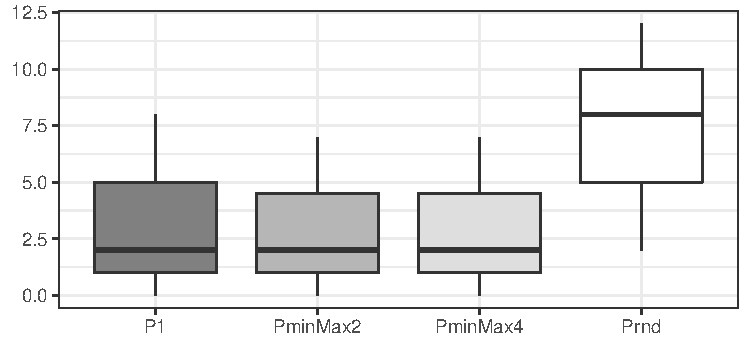
\includegraphics[width=.49\textwidth]{./images/mode_distTA.pdf}
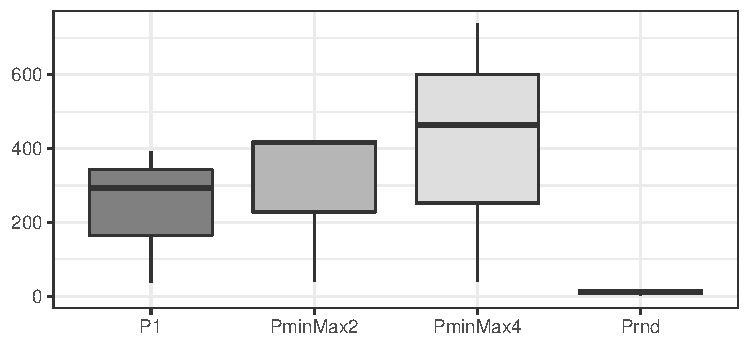
\includegraphics[width=.49\textwidth]{./images/mode_tests.pdf}
\caption{Policy effectiveness in terms of distance of repaired model (left) and of number of generated test traces (right)}
\label{fig:f1ByThs}
\end{figure*}
\end{comment}

\researchquestion{How long does the approach take?}
The time taken by the process depends on the size of \initTa and on the test generation policy. The most expensive phase is the generation of the constraints, as it requires to call \imitator for each test that must be accepted.
As future work, we plan to optimize this phase by modifying \imitator{} to synthesize valuations guaranteeing the acceptance of multiple timed words in a single analysis.
In the experiments, we use as oracle another \ta that we can visit for acceptance; this visit is quite fast and so step \ding{195} does not take too much time. However, in the real setting, the oracle is the real system whose invocation time may be not negligible; in that case, the invocation of the oracle could become a bottleneck and we would need to limit the number of generated tests.


\begin{tikzborder}{}
\begin{figure}[!htb]
	%	\begin{subfigure}[b]{0.49\textwidth}
	\centering
	\footnotesize
	
	\begin{tikzpicture}[scale=1, xscale=1.1, yscale=1.1, auto, ->, >=stealth']
	
	\node[location, initial] at (0, 0) (l1) {$\loc_1$};
	
	\node[location] at (2, 0) (l2) {$\loc_2$};
	
	\node[location] at (4, 0) (l3) {$\loc_3$};
	
	% 			\node[location] at (2, -1) (l4) {$\loc_4$};
	
	\node[location] at (4, -1) (l4) {$\loc_4$};
	
	\node[location] at (6, 0) (l5) {$\loc_5$};
	
	\node[invariant, above=of l1] {$\styleclock{\clock} \leq 4$};
	\node[invariant, above=of l2] {$\styleclock{\clock} \leq 5$};
	\node[invariant, above=of l4] {$\styleclock{\clock} \leq 6$};
	
	\path (l1) edge node[align=center]{$\styleclock{\clock} \leq 3$} node[below]{$\styleact{a}$} (l2);
	\path (l2) edge node[align=center]{$\styleclock{\clock} = 5$} node[below]{$\styleact{b}$} (l3);
	% 			\path (l1) edge[bend right] node[below left, align=center]{$\styleclock{\clock} > 2$ \\ $\styleact{a}$ \\ $\styleclock{y} := 0$} (l4);
	\path (l2) edge node[below left, align=center]{$\styleclock{x} \geq 4$ \\ $\styleact{c}$} (l4);
	\path (l3) edge node[align=center]{$\styleclock{x} \geq 8$} node[below]{$\styleact{d}$} (l5);
	
	\end{tikzpicture}
	%		\caption{Another oracle TA}
	
	
	%	\end{subfigure}
	
	\caption{Repairing TAs with different structures -- Another oracle TA}
	\label{figure:example-TA-different}
\end{figure}
\end{tikzborder}

\researchquestion{Which is the process performance if \ptaProc does not include the oracle?}

\ref{assumption:oracle-in-pta} assumes that the user provides a PTA that contains the oracle. In \ref{ss:discussion-abstraction}, we discussed about the possible consequences when this assumption does not hold. We here evaluate whether the approach is still able to partially repair \initTa using an oracle having a different structure. We took the \ta shown in \ref{figure:example-TA-different} as oracle of the running example, that is structurally different from \initTa and \ptaProc shown in \ref{figure:example} (we name this experiment as \benchmarkExampleShortAlt); the semantic conformance \semConf of \initTa \wrt{} the new oracle is shown at the last row of \ref{table:expResults}\footnote{Note that it does not make sense to measure the syntactical distance, as the structure of the oracle is different.}.
We performed the experiments with the new oracle using the greedy approach described in \ref{assumption:oracle-in-pta}, and results are reported in \ref{table:expOtherOracle}.
%
\begin{table}[!htb]
	\centering
	\caption{Experimental results -- Different oracle}
	\label{table:expOtherOracle}
	\setlength\tabcolsep{2.8pt}
	%\resizebox{\textwidth}{!}{
	\begin{tabular}{lrrrrrrrr}
		\toprule
		Bench. & Policy & \multicolumn{5}{c}{time (s)} & \# failed tests/ & \repTa\\
		\cline{3-7}\cline{9-9}
		& & total & Steps \ding{193}-\ding{194} & Step \ding{195} & Step \ding{196} & Step \ding{197} & \# tests & \semConf (\%)\\
		\midrule
		\benchmarkExampleShortAlt & \policyminusplus & 2.083 & 0.007 & 0.005 & 2.055 & 0.013 & 10/ 44 & 98.72 \\
		\benchmarkExampleShortAlt & \policymiddle & 2.718 & 0.005 & 0.004 & 2.693 & 0.013 & 11/ 47 & 98.72 \\
		\benchmarkExampleShortAlt & \policyquarter & 2.686 & 0.004 & 0.003 & 2.658 & 0.012 & 11/ 47 & 98.72 \\
		\benchmarkExampleShortAlt & \policyrand &  0.763 & 0.007 & 0.001 &  0.676 & 0.075 &   1/  3 &  99.5 \\ 
		\bottomrule
	\end{tabular}
	%}
\end{table}
%
We observe that policies \policyminusplus, \policymiddle, and \policyquarter, although they find some failing tests, they are not able to improve \semConf. This is partially due to the fact that \semConf is computed on some timed words \testDataConf that may be not enough to judge the improvement. On the other hand, as the three policies try to achieve a kind of coverage of \ptaProc (so implicitly assuming \ref{assumption:oracle-in-pta}), it could be that they are not able to find {\it interesting} failing tests (\ie{} they cannot be repaired); this seems to be confirmed by the fact that the random policy \policyrand is instead able to partially repair the initial \ta using only three tests, out of which one fails. We conclude that, if the assumption does not hold, trying to randomly select tests could be more efficient.
\end{tikzborder}

\section{Related Work}\label{sec:related1}

\fakeparagraph{Testing timed automata}
\bb Works related to ours are approaches for test case generation for timed automata. In~\cite{aichernig2013time,aichernig2014debugging}, a fault-based approach is proposed. The authors defined 8 mutation operators for \tas and a test generation technique based on bounded-model checking; tests are then used for model-based testing to check that System Under Test (SUT) is conformant with the specification. Our approach is different, as we aim at building a faithful representation of the SUT (\ie{} the oracle). Their mutation operators could be used to repair our initial \ta, as done in~\cite{arcaini2019achieving}; however, due to continuous nature of \tas, the possible mutants could be too many. For this reason, our approach symbolically represents all the possible variations of the clock guards (similar to ``change guard'' mutants in~\cite{aichernig2013time}). Other classical test generation approaches for timed automata are presented in~\cite{springintveld2001testing,Hessel2008}; while they aim at coverage of a single \ta, we aim at coverage of a family of \tas described by \ptaProc.

%Testing timed automata \cite{springintveld2001testing}

%Mutation-based testing for timed automata \cite{Aichernig2015MMT,aichernig2013time,aichernig2014debugging}

%Other kind of abstraction: Copta models \cite{luthmann2019minimum}

%Feature models \cite{evalUpdateJSS2019}

\vspace{5pt}

\fakeparagraph{Learning timed systems}
In a different direction, learning timed systems has been studied in the past.
Learning consists in retrieving an unknown language, with membership and equivalence queries made to a teacher.
The (timed) language inclusion is undecidable for timed automata~\cite{AD94}, making learning impossible for this class.
In~\cite{GJL10,LALSD14}, timed extensions of the $L^*$ algorithm~\cite{Angluin87} were proposed for event-recording automata~\cite{AFH99}, a subclass of timed automata for which language equivalence can be decided.
Learning is essentially different from our setting, as the system to be learned is usually a white-box system, in which the equivalence query can be decided.
In our setting, the oracle does not necessarily know the structure of the unknown system, and simply answers membership queries.
In addition, we address in our work the full class of timed automata, for which learning is not possible.
\end{tikzborder}


%%%%%%%%%%%%%%%%%%%%%%%%%%%%%%%%%%%%%%%%%%%%%%%%%%%%%%%%%%%%
%%%%%%%%%%%%%%%%%%%%%%%%%%%%%%%%%%%%%%%%%%%%%%%%%%%%%%%%%%%%
\section{Conclusions}\label{sec:conclusions2}
%%%%%%%%%%%%%%%%%%%%%%%%%%%%%%%%%%%%%%%%%%%%%%%%%%%%%%%%%%%%
%%%%%%%%%%%%%%%%%%%%%%%%%%%%%%%%%%%%%%%%%%%%%%%%%%%%%%%%%%%%

\begin{tikzborder}{}
This paper proposes an approach for automatically repairing timed automata, notably in the case where clock guards shall be repaired.
Our approach generates an abstraction of the initial TA in terms of a PTA, generates some tests, and then refines the abstraction by identifying only those TAs contained in the PTA that correctly evaluate all the tests.

As future work, we plan to adopt also other formalisms to build the abstraction where to look for the repaired timed automata;
The CoPtA model~\cite{luthmann2019minimum}, for example, extends timed automata with feature models and allows to specify additional/alternative states and transitions.
In addition, when the oracle acts as a white-box, \ie{} when the oracle is able to test language equivalence, we could also make use of learning techniques for timed automata despite the undecidability of the language inclusion problem, using the almost-always terminating procedure for language inclusion in~\cite{WSLWL14}.

\end{tikzborder}

\part{Tools to Support Model Repair}
\chapter{CTWedge: Migrating Combinatorial Interaction Test Modeling and Generation to the Web}\label{ch:ctwedge}
\begin{tikzborder}{\cite{IWCTGargantini2018}}
Combinatorial Interaction Testing (CIT) is becoming a widespread practice for software testing.
The presence of tools for CIT is of fundamental importance because performing CIT activities manually can be error prone and time consuming. The site pairwise.org\footnote{See \url{http://www.pairwise.org/tools.asp}} lists at least 43 tools supporting several CIT activities while the paper~\cite{NieL11} reviewed the CIT literature and found around 20 tools. 

Most of the tools are classical programs or plugins of existing programs/platforms.  In all these cases, the user has to download, install, and execute the program on his/her machine.  Some tools offer a GUI interface, for example, for defining the models and run the test generation, while others rely on other programs for some activities (like PICTMaster, based on PICT~\cite{czerwonka2006pairwise}, that works entirely inside Microsoft Excel). %(like PICT~\cite{czerwonka_pairwise_2006} that gives the output as an Excel spreadsheet).
In~\cite{citlab12} we have presented a plugin for the eclipse IDE that helps the user in writing CIT models with constraints by leveraging all the expected features of a modern IDE, and it generates combinatorial test suites by using third party programs (like CASA or ACTS).
However, this classical approach poses some challenges. First, the user must install the chosen CIT tool, which in turn may require some dependencies, like java, or in case of plugin, it requires the installation of another program or application like eclipse, excel and so on. Then the user must use his/her machine for running the test generation algorithms. For experienced users with powerful machines they can administer, this is not a real problem. However, for novice users with not so powerful computer, or students that are just learning the CIT principles, or software developers using computer they cannot administer, this can become a cost to be considered and it may be an obstacle for the use of CIT.

Second, from the point of view of tool developers, the distribution of programs means that they have little or no control on the software once is installed: when a bug is discovered the developer has to fix the bug, publish a new version of the tool and hope that the users will update their software. Moreover, the developer has no idea about how the software is used: what are the typical scenarios of use (big or small models, for example), what are the features that are mostly used (for example, what modeling features are more used). Furthermore, it is difficult for tool developers to apply a cost model able to reward their effort in developing and deploying the CIT tool. Indeed, most of the tools are given away for free by researchers supported by their own organization.

A possible solution of these problems could be the offer of CIT features as software as a service (SaaS). SaaS is software that is accessed t+hrough Internet by using a classical web browser.  The SaaS software is actually hosted on the vendor’s servers, and the customers log in and perform tasks as necessary.  The 
vendor is the one who is ultimately responsible for hosting, upgrading and maintaining the program as needed.  There is an extensive literature about SaaS and the advantages (together with limitations) are well known~\cite{Menken:2008}. 

There are already experiences in using the web for CIT. For instance, CTWeb Classic~\cite{usaolaframework}, CTWeb Plus~\cite{ctwebplus}, TestCover~\cite{testcover}, Hexawise~\cite{hexawise}, and PairWiser~\cite{pairwiser}. 

However, as we will discuss in the related work section, each tool has its own specific language to define combinatorial models, with its own predefined output formats and a (limited) set of supported existing or in-house algorithms for test case generation. Not all those tools are equally powerful or easy to use, and many of them are commercial or require registration.

For this reason, starting from our experience with \citlab~\cite{citlab12}, we have worked on a web based application that allows the user to write CIT models in a similar way he/she would do in a classical IDE and it offers test suite generation by means of   server using known and community evaluated test generation algorithms. 
Our system, called \ctwedge (Combinatorial Testing Web EDiting and GEneration), introduces a rich language for combinatorial models, offers a powerful web editor, and allows the user to generate the CIT test suites on a server. The only software needed to use \ctwedge is a modern web browser.

The paper is organized as follows. In Sect. \ref{sec:language} we present the modeling language (in an abstract way) we use to define CIT models. In Sect. \ref{sec:ctwedge} we introduce our tool, its architecture, its web editing capabilities, and the generator engine. A detailed comparison with other similar web based tools is presented in  Sect. \ref{sec:related2}. Future works and possible directions of extension are presented in Sect. \ref{sec:futurework}. Sect. \ref{sec:conclusions3} concludes the paper.
\end{tikzborder}

\section{A simple language for CIT models}\label{sec:language}

\begin{tikzborder}{}
We have devised a simple textual language for CIT models which is suitable to be used in web editors. It allows the definition of parameters, each with its name and (finite) domain, and it is based on our previous language defined for \citlab \cite{citlab12}. We allow the following parameter types: 

\begin{enumerate}
	\item \textsf{Boolean} with only two possible values \textsf{true} and \textsf{false} (all lower or all upper case).
	The two boolean constants are also considered of Boolean type.
	\item \textsf{Ranges} that are integer intervals defined by their lower bound $l$ and upper bound $u$. With $[l..u]$ we denote all the integers between $l$ and $u$ included.
	\item \textsf{Enumerative} that are a list of possible values between \{\}. We are rather liberal about the elements and we allow identifier starting also with a number, natural numbers, and strings. For example, one could define a  enumerative \textsf{values} in this way:
	\begin{lstlisting}[language=ctwedge]
	values : {100, 1M, "my name", cit}
	\end{lstlisting}
\end{enumerate}

A simple example of combinatorial model with three parameters is shown in Fig. \ref{fig:ctexample}. 
\end{tikzborder}

\begin{figure}[htb]
	\centering
	\begin{lstlisting}[language=ctwedge,frame= single]
	Model Phone
	Parameters:
	emailViewer : Boolean
	textLines:  [ 25 .. 30 ]
	display : {16MC, 8MC, BW}
	\end{lstlisting}
	\caption{A smartphone example}
	\label{fig:ctexample}
\end{figure}

\begin{tikzborder}{}
There are some semantic rules about the parameters and their definitions, defined as follows:
\begin{enumerate}
	\item The name of each parameter must be unique.
	\item In \textsf{Ranges}, the lower bound $l$ must be less than the upper bound $u$.
	\item The elements in each \textsf{Enumerative} must be distinct. We allow two enumerative parameters to share some elements, though.
\end{enumerate}
\end{tikzborder}

\subsection{Constraints}

\begin{tikzborder}{}
A distinctive feature of our language is the support of modeling constraints among parameters. 
In most configurable systems, constraints or dependencies exist between parameters. 
Constraints may be introduced for several reasons, for example, to model inconsistencies between certain hardware components, limitations of the possible system configurations, or simply design choices~\cite{CohenISSTA07}.
In our approach, tests that do not satisfy the constraints are considered \emph{invalid} and do not need to
be produced. 
For this reason, the presence of constraints may reduce the number of tests of the final test suite (but it may also increase it ~\cite{CohenISSTA07}).
However, the generation of tests considering constraints is generally more challenging than the generation without them, and several test generation techniques still do not support constraints, at least not in a direct manner.
In \ctwedge we decided to focus more on techniques supporting constraints.

In \ctwedge, we adopt the language of propositional logic (with the usual logical operators) with equality and arithmetic to express constraints. 
To be more precise, we use propositional calculus, enriched by the arithmetic over the integers and enumerative symbols. As operators, we admit the use of equality and inequality for any variable, the usual Boolean operators for Boolean terms, and the relational and arithmetic operators for numeric terms. 
To be more precise, Table \ref{tab:validity} reports all the rules we have defined to check if a constraint is semantically correct.
\end{tikzborder}

\begin{table*}
	\centering
	\resizebox{\textwidth}{!}{
	\begin{tabular}{|l|l|l|}
		\hline 
		\textbf{Expression}	& \textbf{Case} & \textbf{Correct iff}\\\hline
		\multirow{7}{*}{\shortstack{$e_1\ op\ e_2$	with $op \in \{=, \neq \}$ $\rightarrow boolean$ \\ $ e_2\ op\ e_1$ with $op \in \{=, \neq \}$ $ \rightarrow boolean$ }}  & $e_1$ enumerative, $e_2$ element& $e_2$ belongs to $e_1$ elements \\\cline{2-3}
		
		& $e_1$ enumerative, $e_2$  enumerative& $e_1$ and $e_2$ share at least one element \\\cline{2-3} 
		&  $e_1$ range, $e_2$ range & $e_1$ and $e_2$ share at least one number \\\cline{2-3}
		& $e_1$ range, $e_2$ number & always \\\cline{2-3}
		& $e_1$ number, $e_2$ number & always \\\cline{2-3}
		& $e_1$ boolean, $e_2$ boolean & always\\\cline{2-3}
		\hline 
		
		\multirow{3}{*}{\shortstack{$e_1\ op\ e_2$	with $op \in \{<, \le, >, \ge \}$ $\rightarrow boolean$ \\ $ e_2\ op\ e_1$ with $op \in \{<, \le, >, \ge \}$ $ \rightarrow boolean$ }}  &  $e_1$ range, $e_2$ range & $e_1$ and $e_2$ share at least one number \\\cline{2-3}
		& $e_1$ range, $e_2$ number & always \\\cline{2-3}
		& $e_1$ number, $e_2$ number & always \\\cline{2-3}
		\hline 
		
		\multirow{3}{*}{\shortstack{$e_1\ op\ e_2$	with $op \in \{\wedge, \vee, \rightarrow\}$ $\rightarrow boolean$ \\ $ e_2\ op\ e_1$ with $op \in \{ \wedge, \vee, \rightarrow \}$ $ \rightarrow boolean$ }}  & \multirow{3}{*}{$e_1$ boolean, $e_2$ boolean} & \multirow{3}{*}{always} \\ %\cline{2-3}
		& & \\
		& & \\ 
		\hline
				
		\multirow{1}{*}{$\neg e$ $ \rightarrow boolean$}  & $e$ boolean & always \\\cline{2-3}
		\hline
		
		\multirow{4}{*}{$e_1\ op\ e_2$	with $op \in \{+, -, *, /, \%\}$ $\rightarrow number$}  & $e_1$ number, $e_2$ number & $e_2 \neq 0$ if $op=/$ or $op=\%$ \\\cline{2-3}
		& $e_1$ range, $e_2$  range & always \\\cline{2-3} 
		&  $e_1$ range, $e_2$ number & $e_2 \neq 0$ if $op=/$ or $op=\%$ \\\cline{2-3}
		&  $e_1$ number, $e_2$ range & always \\\cline{2-3}
		\hline
	\end{tabular} 
}
	\caption{Rules of \ctwedge Language Validator for Constraints}\label{tab:validity}
\end{table*}

\begin{tikzborder}{}
For example, we can write constraints in this way:
\end{tikzborder}

\begin{lstlisting}[language=ctwedge,frame= single]
Model Phone
..
Constraints:
# emailViewer => textLines > 28 #
# emailViewer and display != 16MC => textLines > 28 + 3#
\end{lstlisting}

\begin{tikzborder}{}
Many test suite generation tools provide a limited support for constraints. For instance, AETG \cite{AETG,Lott2005} allows only simple constraints of type \textsf{if then else} or \textsf{requires}. The language of \ctwedge is in this aspect more expressive, as it is targeted to be more general than existing tools. In the specific case of AETG, the translation of those templates into our logic is straightforward. For example the \textsf{if then else} constraint can be translated by two implications.
Other tools \cite{CohenISSTA07} allow constraints only in the form of forbidden combinations \cite{Golumbic:2011:GTC:2028636}. Our language is more general, as a forbidden tuple would be translated as a \textit{not} statement. For instance, a forbidden pair \textsf{emailViewer = false; display = 16MC} would be represented by the following constraint:
$$\textsf{\#\ not\ (emailViewer = false\ and\ display = 16MC)\ \#}$$
However, the explicit list of the forbidden combinations may explode and it may become impractical and error-prone to represent it. For example, if the model of mobile phones presented in Fig. 1 had a constraint that

\emph{"A front video camera requires also a 16MC display"}. This constraint would be translated into two forbidden tuples:

$$\textsf{(emailViewer = true, display = 8MC);}$$
$$\textsf{(emailViewer = true, display = BW);}$$
However, the translation as constraint in general form would be simply:
$$\textsf{\#\ emailViewer =\textgreater\ display = 16MC\ \#}$$
which is more compact and more similar to the informal requirement.

In our language semantics, a test case is valid only if it does not contradict any constraint in the specification. Others \cite{BRYCE2006960} distinguish between combinations to be avoided \textit{if possible} (soft constraints), and the forbidden combinations (hard constraints), which must always be avoided (our case). %We consider only hard constraints, for now.

Other tools, like CASA \cite{CASAwebsite}, support only constraints in conjunctive normal form, without arithmetic or relational operators.
\end{tikzborder}

\subsection{Xtext}

\begin{tikzborder}{}
There are countless ways to define a language together with its parser. One emerging technique for Domain Specific Language modeling is the use of Xtext~\cite{Eysholdt:2010}. By defining the grammar of the DSL of choice by means of a Xtext grammar, the language designer obtains a parser, APIs to programmatically access models, a serializer and a smart editor for it. The editor provides many features out-of-the-box, such as syntax highlighting, content-assist, folding, jump-to-declaration and reverse-reference lookup across multiple files.  We had already used Xtext for defining the language in \citlab~\cite{citlab12}. Xtext support also the generation of a web editor, as we present in the following section.

Grammar rules written in Xtext are very close to the standard (E)BNF production rules. For instance, the main grammar rule that defines the whole CIT model is defined as follows:
\end{tikzborder}

\begin{lstlisting}[language=Matlab,columns=fullflexible,basicstyle=\small\ttfamily,stringstyle=\ttfamily\color{blue},upquote=true]  
CitModel:
'Model' name=ID 
'Parameters' ':' (parameters+=Parameter)+ 
('Constraints' ':' (constraints+=Constraint)+)?
\end{lstlisting}

\begin{tikzborder}{}
Xtext can display the production rules by means of syntax diagrams, also known as railroad diagrams. For example, the rule presented before for {\small\ttfamily CitModel} is shown in Fig. \ref{fig:grammarrule}.
\end{tikzborder}

\begin{figure}
	\centering
	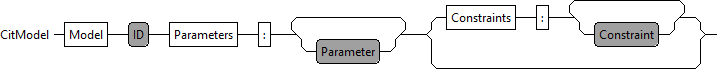
\includegraphics[width=1\linewidth]{images/grammar_rule}
	\caption{{\small\ttfamily CitModel} rule diagram}
	\label{fig:grammarrule}
\end{figure}

\begin{tikzborder}{}
Because Xtext is based on ANTLR, it does not allow left recursive parser rules and parsing nested expressions is not as simple as writing a EBNF rule. The \ctwedge language parses the constraints by defining the precedence among operators implicitly by left-factoring expression definitions. For example, in order to parse the AND operators before the OR operators,  \ctwedge  introduces the following two rules that are not left recursive:
\end{tikzborder}

\begin{lstlisting}[language=Matlab,columns=fullflexible,basicstyle=\small\ttfamily,stringstyle=\ttfamily\color{blue},upquote=true,morekeywords={returns}]  
OrExpression returns Expression:
AndExpression ({OrExpression.left=current} 
OR_OPERATOR (right=AndExpression))*;

AndExpression returns Expression:
EqualExpression ({AndExpression.left=current}
AND_OPERATOR (right=EqualExpression))*;
\end{lstlisting}


\begin{tikzborder}{}
The definitions of semantic constraints in Xtext is performed by user-defined validator classes written in Java or in Xtend containing methods annotated by {\small\ttfamily @Check}. For instance, to check that in the definition of any range domain of our CIT models  the upper bound is greater than the lower bound, we have introduced the following checking method:
\end{tikzborder}

\begin{lstlisting}[language=Java,morekeywords={def},basicstyle=\small\ttfamily]
@Check
def checkRangeIsCorrect(Range range) {
if (range.getBegin() >= range.getEnd())
error("The second term must be greater ...");
}
\end{lstlisting}

\section{\ctwedge: CT Web Editor and Generator}\label{sec:ctwedge}

\begin{tikzborder}{}
In this section, we present our tool \ctwedge. 
As we can see in Fig.~\ref{fig:architecture}, the tool is composed by a language definition component (with its Xtext parser and validator), a web-based editor for the \ctwedge language, with some options for test generation and a test suite visualizer and exporter, and a test suite generator that exploits third-party test generation tools.

The tool is written in Java and Xtext, and can be deployed on any Web-application server, such as Apache Tomcat. It is publicly available at: \url{http://foselab.unibg.it/ctwedge/}.
\end{tikzborder}

\begin{figure}[bt!]
	\centering
	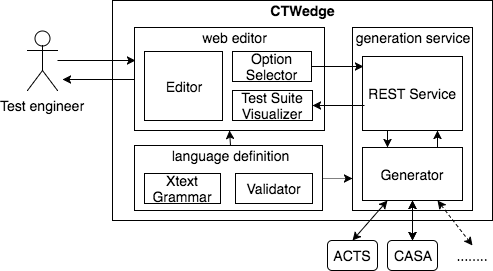
\includegraphics[width=.8\columnwidth]{images/architecture.png}
	\caption{\ctwedge architecture}\label{fig:architecture}
\end{figure}

\subsection{Combinatorial Testing Web Editor}

\begin{tikzborder}{}
In order to implement a web-based editor, we can leverage the Xtext framework, since Xtext starting from version 2.9 offers an interface for integration of text editors in web applications. The text editors are implemented in JavaScript, and language-related services such as code completion are realized through HTTP requests to a server-side component.

The Xtext web-based editor provides several features, like content assist to help the user to complete the models, validation to check the correctness, syntax coloring, and formatting.

The \ctwedge web editor is based on Ace (Ajax.org Cloud9 Editor)\footnote{See \url{https://ace.c9.io/}}, but other web editors (like Orion and CodeMirror) are available. Xtext does not yet provide support for the recently standardized Language Server Protocol \cite{lsp}, which we plan to include in our tool as a future work.  A screenshot of the \ctwedge web editor is shown in Fig. \ref{fig:editor}. The web editor provides an immediate feedback while writing by means of syntax highlighting, auto completion, and errors markings. 

The validation of the model is performed run-time while the user writes it. If the validator finds an error in the model, it generates an error message. The nature of the error is indicated in the pop-up box appearing when positioning the cursor over the error sign, and the point in which the error occurs is marked in the editor. Fig. \ref{fig:validation} shows how model validation errors are displayed to the test engineer.
\end{tikzborder}
\begin{figure*}[bt!]
	\centering
	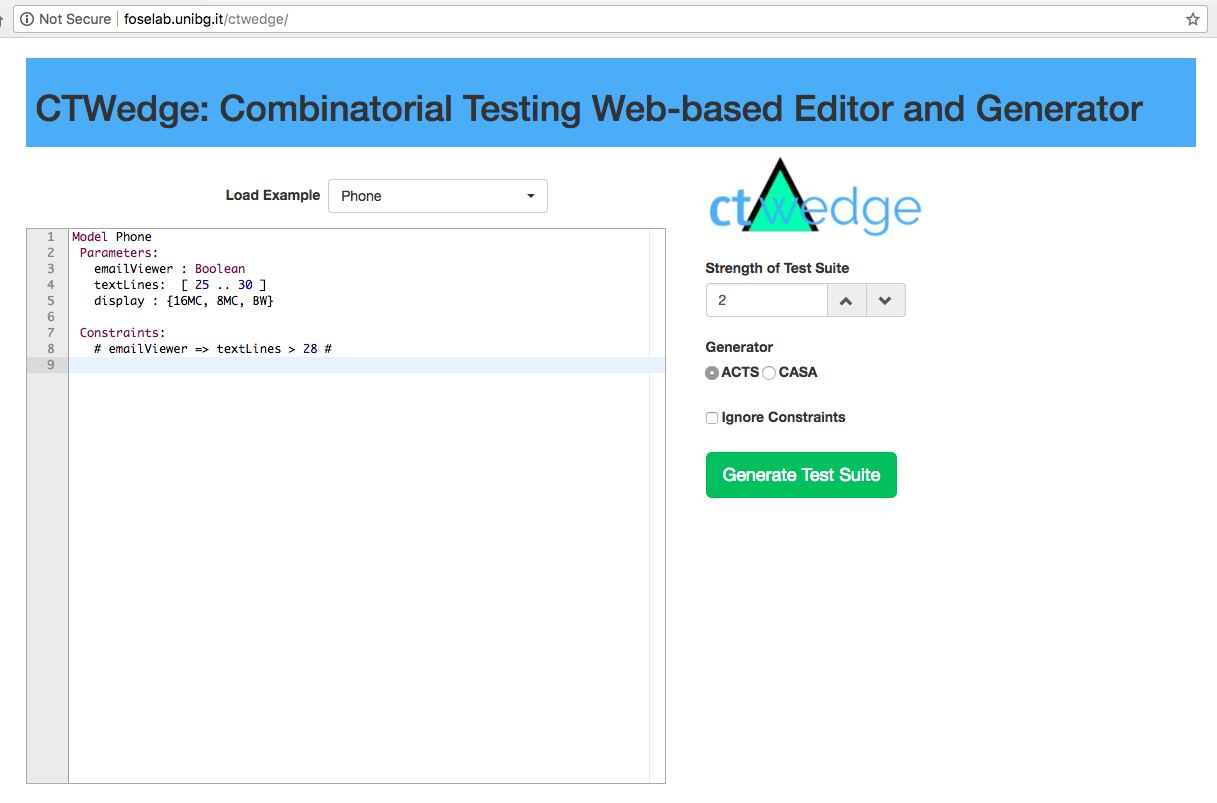
\includegraphics[width=\textwidth,trim={0 10cm 0 0},clip]{images/editor2.png}
	\caption{\ctwedge web editor}\label{fig:editor}
\end{figure*}

\begin{tikzborder}{}
The editor allows to load predefined examples of combinatorial models, selected from literature \cite{segall_using_2011} and converted into \ctwedge language format (with extension \textit{.ctw}).

Graphical components (buttons and option selectors) are built using the JavaScript frameworks JQuery\footnote{JQuery: \url{https://jquery.com/}}
and Bootstrap\footnote{Bootstrap: \url{https://getbootstrap.com/}}.
The web application is fully compatible also with mobile devices (Android and iOS), from any recent Web browser with JavaScript enabled.
\end{tikzborder}

\begin{figure}[bt!]
	\centering
	\begin{subfigure}{\columnwidth}
		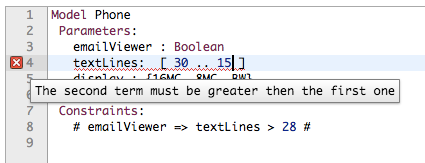
\includegraphics[width=.6\columnwidth]{images/validation1.png}\caption{Validation of Range parameter}
	\end{subfigure}
	
	\begin{subfigure}{\columnwidth}
		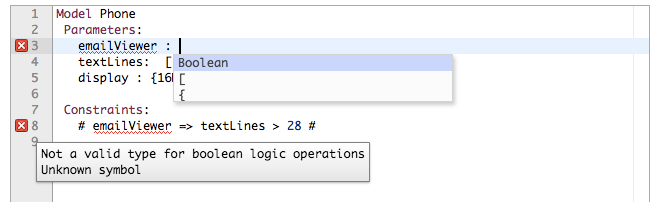
\includegraphics[width=.8\columnwidth]{images/validation2.png}\caption{Code recommender. Unknown symbol error.}
	\end{subfigure}
	
	\begin{subfigure}{\columnwidth}
		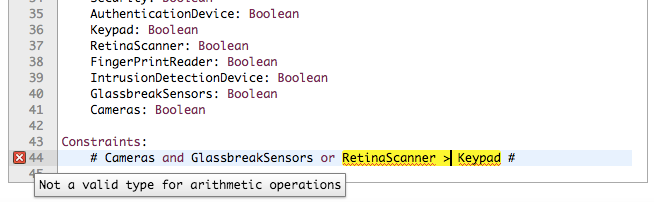
\includegraphics[width=.65\columnwidth]{images/validation3.png}\caption{Validation of relational operations}
	\end{subfigure}
	\caption{Examples of \ctwedge validation errors}\label{fig:validation}
\end{figure}


\subsection{Test generator web service}

\begin{tikzborder}{}
The function of actually generating a test suite from the test model and option parameter is web-served and performed by the test generation service which is the component of \ctwedge.
The test generation service is composed by two modules: a REST\footnote{REST: Representational State Transfer} service and a language translator.

The REST service handles input model and option parameters for the generation, calls the generators from which it gets back the tests and it is responsible to deliver them to the web browser. 

The test generator acts as a \textit{driver} between \ctwedge and the various third party combinatorial test generation tools, which are usually accessible via their own APIs, or via command line. The test generator exports the combinatorial model along with the generator options, into the the specific language of the external tool, or directly into the tool's APIs. Then, it waits for the generator to compute the test suite, and once ready, it passes it back to the REST service. If necessary, the generator also maps any parameter values back to the original \ctwedge model format. Each external program needs its own translator.
\end{tikzborder}

\begin{table}[!htb]
	\caption{Request parameters to \ctwedge generation service}
	\centering
	\footnotesize
	\resizebox{0.8\textwidth}{!}{%
		\centering
		\begin{tabular}{l l p{2.55cm} p{3.35cm}}
			\toprule
			\textbf{Parameter} & \textbf{type} & \textbf{description} & \textbf{values} \\
			\midrule
			model & String & the combinatorial model & as written and validated by the editor (see Sec. \ref{sec:language}) \\ 
			strength & Int & the combinatorial interaction strength & any integer above 1 (default is 2: pairwise) \\ 
			generator & Enum & the tool to be used & ["acts", "casa"] (so far) \\
			ignConstr & Boolean & if constraints should be ignored in test generation & ["true", "false"] (default is false) \\ 
			\bottomrule
		\end{tabular}
	}
	\label{tab:parameters}
\end{table}

\begin{tikzborder}{}
The REST service accepts an HTTP GET or POST request with parameters as described in Tab. \ref{tab:parameters}.
For sake of brevity, an example URL request to the web generator service is shown in Fig. \ref{fig:urlexample}.
\end{tikzborder}

\begin{figure}[htb!] % https://tex.stackexchange.com/questions/116534/lstlisting-line-wrapping
	\centering
	\lstset{
		basicstyle=\ttfamily\small,
		columns=fullflexible,
		frame=single,
		breaklines=true,
		postbreak=\mbox{\textcolor{red}{$\hookrightarrow$}\space},
		language=url
	}
	\begin{lstlisting}
	http://foselab.unibg.it/ctwedge.generator?model=Model%20Phone%20Parameter:%20...>28%20#&strength=2&generator=acts&ignConstr=false	
	\end{lstlisting}
	\caption{Generator URL example}
	\label{fig:urlexample}
\end{figure}

\begin{tikzborder}{}
So far, we interfaced \ctwedge with ACTS~\cite{ACTS} and CASA~\cite{CASAwebsite}. ACTS is accessed  via it internal APIs whereas CASA is called via command line.

The resulting test suite is returned in CSV\footnote{CSV: Comma Separated Values} format. The header line contains the parameter names, and each following line represents a single test, with parameter values.
The web front-end allows to download CSV file to further local use, and shows the test suite in the browser by converting it into an HTML table. Conversion is straightforward and done client-side via Javascript.

Arithmetic operations and relational operators ($>$, $<$, $\le$, $\ge$) are not natively supported by CASA, and in presence of such constraints, an error is reported to the user, as in Fig. \ref{fig:casaError}.
\end{tikzborder}

\begin{figure}[hbt!]
	\centering
	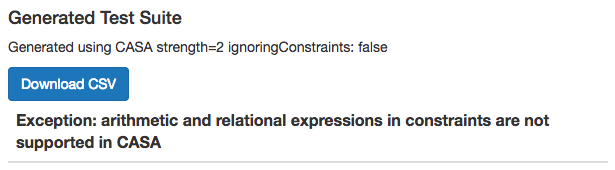
\includegraphics[width=\columnwidth]{images/casaError.png}
	\caption{Message of operations not supported in constraints for CASA generator tool}\label{fig:casaError}
\end{figure}

\begin{figure}[hbt!]
	\centering
	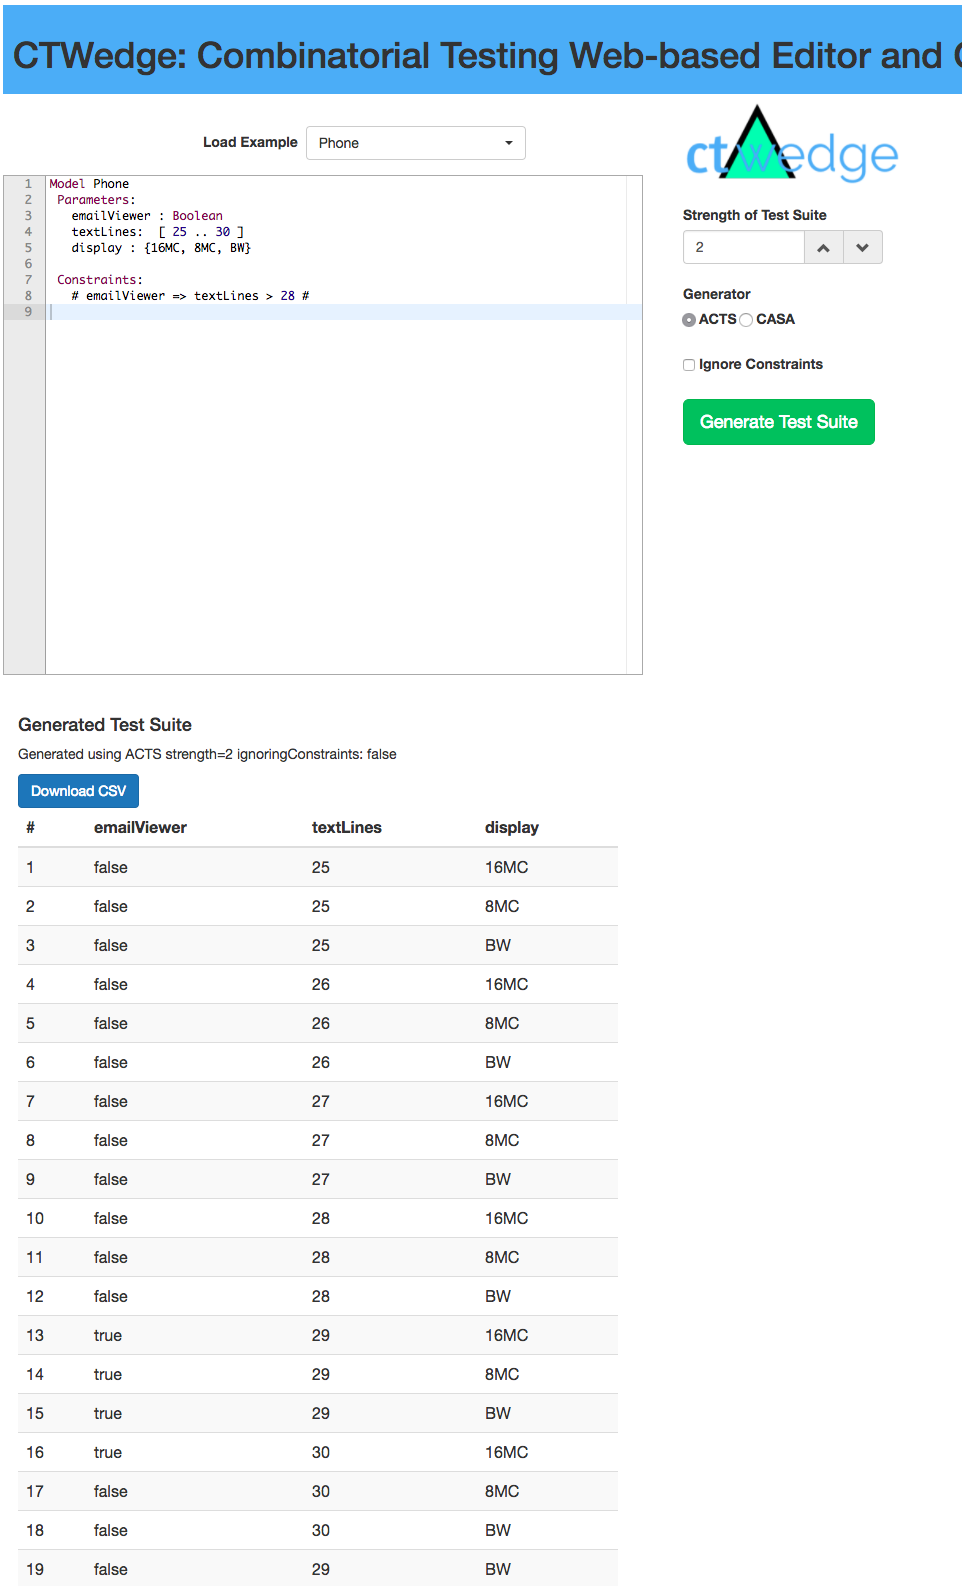
\includegraphics[width=.5\columnwidth,trim={0 0 7cm 0},clip]{images/generatedTable.png}
	\caption{\ctwedge visualization of the generated test suite}\label{fig:generated}
\end{figure}

\begin{tikzborder}{}
The HTML table showing the generated test cases is located below the editor on the same window. This location is less invasive than a brand new tab as it does not hide or replace the current combinatorial model in the editor. Despite it is not immediately visible to the user, who may think the output is hidden, we believe that it preserving the access to the current screen is the most important aspect to be preserved.

The generator is called by the editor by AJAX, with an asynchronous XmlHttpRequest.

A screenshot of how the generated test suite is presented to the user is shown in Fig. \ref{fig:generated}. 
It is shown as plain HTML table, with the possibility to download the data as CSV. 
\end{tikzborder}

\section{Related Work}\label{sec:related2}

\begin{tikzborder}{}
With the success of the SaaS pattern, web-based tools have rapidly gained popularity due to their portability and ease of use. There exist some web-based services also for combinatorial test case generation, each with its own peculiarities. SaaS tools, however, still represents a small number of all the available tools for test case generation: IDE plugins and desktop applications represent almost the totality of the current tools. We looked for tools from the pairwise.org\footnote{See \url{http://www.pairwise.org/tools.asp}} and softwaretesters.net\footnote{See \url{https://softwaretesters.net/zbxe/index.php?mid=downloadtool&category=4258006&sort_index=readed_count&order_type=desc}} tool catalogs, and from the web, to the best of our searching skills. 
\end{tikzborder}

\begin{table}[!hbt]
	\centering
	\footnotesize
	\setlength\tabcolsep{2pt}
	\begin{tabular}{l P{52mm} P{52mm}}
		Tool & URL & Documentation \\
		\toprule
		TestCover & \url{https://testcover.com} & \url{https://testcover.com/sub/instructions.php} (visible after registration) \\
		\midrule
		CTWebClassic & \url{http://alarcostest.esi.uclm.es/CombTestWeb/combinatorial.jsp} & \url{http://alarcostest.esi.uclm.es/CombTestWeb/stuff/usersManual.pdf} \\
		\midrule
		CTWebPlus & \url{http://www.testcasegeneration.com} or \url{http://www.ctwebplus.com/} & \url{http://www.ctwebplus.com/stuff/userManual.pdf} \\
		\midrule
		HexaWise & \url{https://hexawise.com/} & \url{https://hexawise.com/Hexawise_Introduction.pdf} \\
		\midrule
		PairWiser & \url{https://inductive.no/pairwiser/} & \url{https://inductive.no/pairwiser/knowledge-base/} \\
		\bottomrule
	\end{tabular}\caption{Tool resource links}\label{tab:docs}
\end{table}

\begin{tikzborder}{}
We compare the following five SaaS for CIT, listed in Tab. \ref{tab:docs}:
\begin{itemize}
	\item TestCover~\cite{testcover} is a commercial web-based combinatorial test case generator supported by Testcover.com, LLC, founded in 2003. The tool was also presented at IWCT 2016~\cite{sherwood2016embedded}.
	\item CTWeb Classic~\cite{usaolaframework} is a free online tool for combinatorial testing and state machine test case generation,  developed at University of Castilla-La Mancha (Spain).
	\item CTWeb Plus~\cite{ctwebplus}, an academic combinatorial test generation tool developed as improvement of CTWeb Classic. CTWeb Plus is now commercially supported.
	\item HexaWise~\cite{hexawise}, a commercial combinatorial test case editor and generator, launched in 2009 by Hexawise, Inc.
	\item PairWiser~\cite{pairwiser}, a commercial web-based tool provided by Inductive AS. The online version was shut down January 15th, 2018. After that date, only the standalone application, for own-server installation, is available.
\end{itemize}

All tools are well documented, with examples and tutorials. Links of on-line editors and official documentation resources of these tools are shown in Tab. \ref{tab:docs}
\end{tikzborder}

\begin{table*}[!hbt]
	\resizebox{\textwidth}{!}{%
	\centering
	\setlength\tabcolsep{1pt}
	\tiny
	\begin{tabular}{p{1mm}lP{24mm}P{24mm}P{24mm}P{24mm}P{24mm}P{24mm}}
		%\hline
		& & \centering\textbf{TestCover}~\cite{testcover} & \centering\textbf{CTWeb Classic}~\cite{usaolaframework} & \centering\textbf{CTWeb Plus}~\cite{ctwebplus} & \centering\textbf{HexaWise}~\cite{hexawise} & \centering\textbf{PairWiser}~\cite{pairwiser} & {\textbf{\centering \ctwedge}} \\%\toprule
		\hline 
 
		\multicolumn{2}{l}{\textbf{Language}} & & & & & & \\ 	
		&	Parameter Definition & Enumerative & Enumerative & Enumerative & Enumerative, Ranges (via value expansion) & Enumerative & Boolean, Enumerative, Ranges \\%\midrule
		&	Constraints format & in DPB notation: via \emph{blocks} (i.e., sets of allowed combinations) & as \emph{if-then-else} & AND, OR, Else operators, not nested & invalid pairs (\emph{if..then..}) & guided by select boxes with rich choice of operators & arbitrary formula \\%\midrule
		
		&	Numeric operators & \cmark (in PHP functions) & \xmark & \cmark & \cmark & \xmark & \cmark \\%\midrule
		
		&	State Machine support & \cmark & \cmark & \cmark & \xmark & \xmark & \xmark \\\toprule 
		\textbf{Editing} & & & & & & \\
		&	Web-based editor & text area & text fields and buttons + file upload & text fields, buttons, drawing area & text fields and buttons & text fields and buttons & text area \\%\midrule
		&	Model Import/Export	& \cmark (Copy\&Paste as text) & \cmark & \xmark & \xmark & \xmark & \cmark   (Copy\&Paste as text)\\%\midrule	
		&	Helping facilities & \xmark & button-guided (no facilities to build input file to upload) & button-guided & button-guided & button-guided & content-assist, syntax highlight, in-line error reporting \\%\midrule 
		&	Example Models & \cmark & \cmark & to be rebuilt from documentation file, not one-click loadable & \cmark & in the documentation & \cmark \\\toprule
		
		\multicolumn{2}{l}{\textbf{Generation}} & & & &  & & \\%\midrule 
		&	n-wise & pairwise & pairwise & pairwise & up to 6-way interaction + mixed strength & up to 3-way interaction + mixed strength & \cmark \\%\midrule
		&	Supported generators & All-pairs & AETG, PROW, All combinations, Each choice, Random, Bacteriologic & AETG, Pairwise, All-combinations, Each-choice, Comb, Random & not specified & not specified & ACTS, CASA \\%\midrule
		&	Export formats & HTML, WSDL interface & HTML, CSV & HTML & HTML, Excel, CSV, OPML & Excel, Jira issues & CSV, HTML \\%\midrule
		&	Generate test scripts & \cmark (for Selenium) & \cmark (custom) & \cmark (custom) & \xmark & \cmark (custom) & \xmark \\%\midrule
		&	Coverage visualization & \cmark & \xmark & \xmark & \cmark & \cmark & \xmark \\\toprule 
		\multicolumn{2}{l}{\textbf{Other information}} & & & & & & \\%\midrule
		&	License & Commercial & Free & Commercial & Commercial & Commercial & Free \\%\midrule
		&	Registration & subscription required &  optional & subscription required & subscription required & own-server installation & \xmark \\%\midrule
		&	Online storage & \cmark & \xmark & \cmark & \cmark & \cmark (on own server) &\xmark  \\%\midrule
		&	Additional notes & Functions in PHP into constraints. Also accessible via WSDL interface.
		& Registration required for models with more than 5 parameters & Features a drawing area to represent states and transition of a state machine. The combinatorial model must be in the form of a state machine. & Has also a chart showing the interaction coverage after each test & Pairwiser online was shut down January 15, 2018. Available only for own-server installation. Allows to specify combinations to include in test suite. & -- \\\bottomrule 
	\end{tabular}
	}
	\caption{A comparison with other SaaS for CT}\label{tab:comparison}
\end{table*}

\begin{tikzborder}{}
To compare the SaaS tools among them and w.r.t. \ctwedge, we consider the following aspects, that we believe to be among the most relevant for a test engineer interested in using a web-based combinatorial test generation tool:

\begin{itemize}
	\item \textbf{Language}. We look into the expressiveness of the accepted format for the combinatorial model in input. This evaluation includes:
	\begin{itemize}
		\item Parameter definition: how the parameter types and values  can be defined. For instance, a tool may support Boolean parameters or ranges of integers to express an enumerative made of all integers between two numbers.
		\item Constraint format: if the constraints can be expressed as free combinations of logical and arithmetic operations among parameters, or have special formats, such as a set of forbidden tuples, a set of implications, or a set of if-then-else conditions. 
		\item Numeric Operations: if constant numbers and basic numeric operations (+, -, *, /) are allowed in the constraints and/or in the generated code of test cases.
		\item State Machine support: if the language supports an easy input of state machines, to generate combinatorial tests for their execution.
	\end{itemize} 
	\item \textbf{Editing}. We evaluate how simple is for the test-engineer to input the combinatorial model into the tool. This category includes the following aspects:
	\begin{itemize}
		\item Web-based editor structure: how is the GUI of the web editor for writing the combinatorial model to be given in input to the tool; for example, if it is made by a single text area, or some buttons and text fields. Some tools use a single text area for the whole model, whereas some other tools use text inputs for individual parameters, reducing the need for parsing and text-highlighting.
		
		\item Import and export models: how the models can be exported to the file system and imported. For example, a tool may allow importing a text file written with another editor.
		
		\item Helping facilities: how the test engineer is guided in the input of the model in the web editor; for example with syntax highlighting, content assist, in-line error reporting, warning messages, or single text input fields to fill, and self-explanatory buttons to click.
		\item Predefined example models: if there are examples of combinatorial models that can be easily loaded into the tool and executed to generate a test suite.
	\end{itemize} 
	\item \textbf{Generation}. We evaluate how the test suite generation is performed and how the output is presented to the user. This category includes the following aspects:
	\begin{itemize}
		\item n-wise: which interaction strengths of the generated test suite are allowed
		\item supported generators: which existing combinatorial test generation algorithms are supported
		\item export formats: in which formats the output is made available to the test-engineer
		\item Test-script generation: if there is a mechanism to allow the generated test vectors to be directly inserted into test cases written in custom code.
		\item Coverage visualization: if there is indication (textual or with charts) of the coverage reached after the execution of each test in the generated test suite.
	\end{itemize} 
	\item \textbf{Other information}. We consider aspects about the accessibility of the tool, and related features. We look the following aspects
	\begin{itemize}
		\item License: if commercial, free, or open source.
		\item Registration: if it is mandatory, optional or not made available.
		\item Online storage: if any data (input models, or output test suites) can be stored online.
		\item Additional notes: any other additional information that we consider worth being noted.
	\end{itemize} 
\end{itemize}

Table \ref{tab:comparison} compares the five tools and \ctwedge according to all these aspects.

Concerning the web editor, while TestCover uses, as \ctwedge, a single text area for combinatorial model input,  all the others (CTWeb Classic, CTWeb Plus, HexaWise and PairWiser) feature a composer of combinatorial model guided by multiple selectors, text fields, and buttons. This approach of using buttons and text input fields, has the advantage of a quicker learning curve, and it does not need a language grammar, nor a parser, nor the helping facilities typical of text-based editors, such as auto-completion and syntax highlighting. However, it is not always the preferable way to input combinatorial models in the tool. In fact, the availability of a domain-specific language makes it possible to quickly and easily write, edit and copy-paste combinatorial input models, and export, translate or port them to other platforms and tools.


CTWeb Classic comes both with a guided editor and a form to upload a text file containing the input of the tool, written in a domain specific language. Regarding the textual way of proving input for test case generation, however, although CTWeb Classic and TestCover have a good documentation, they have no facilities to help the test engineer in writing models. CTWeb Classic does not have an online editor for its own language (as it comes with just a file upload button), and TestCover has a simple text area, lacking support for auto-completion, syntax-highlighting and all the features proper of an IDE.

All the tried tools offer support for test case generation with constraints, to be specified in their specific formats.  TestCover even allows to specify custom functions - in PHP code - to express constraints~\cite{sherwood2016embedded}.

TestCover and CTWeb (Classic and Plus) offer pairwise test case generation, that is very often the chosen interaction strength by test-engineers. For some applications, however, higher interaction strength is preferred. HexaWise supports up to 6-way interaction strength, while PairWiser up to 3-way. \ctwedge is, instead, the only tool that does not pose limitation (in theory) on the interaction strength of the test suite. However, HexaWise and PairWiser come with the additional possibility to specify a mixed test suite strength, i.e., values of each single parameter may be covered with different strength.

Still none of the tools supports the Microsoft Language Server Protocol \cite{lsp}, a new common open protocol for language servers which provides programming language-specific features to source code editors or integrated development environments (IDEs). The main goal of the standard is to support programming in any given language independently of editors or IDEs. We plan to extend \ctwedge in order to support LSP.
\end{tikzborder}

\section{Future Work}\label{sec:futurework}

\begin{tikzborder}{}	
There are several directions in which we plan to work. 

\paragraph{Language extensions}
Adding expressive power to the language for combinatorial models, in particular to express test seeds and goals, represents a direction for future work.
Test seeds allow a tester to force the inclusion of certain test cases in the generated test suite \cite{BRYCE2006960}. Test seeds may be complete or partial. 
Test goals are extra-constraints: relations among parameters to be satisfied by at least one test in the generated test suites.

Some CIT approaches \cite{segall_using_2011} introduce weights for parameter values. Weights reflect the importance of different values for a given parameter. The user can express further requirements over the solution involving weights. Even if the same constraints may be expressed in our language, it may become impractical. We plan to extend the \ctwedge language in order to include user defined functions depending on parameter values. A possible function could be the weight of a parameter. Constraints and test goals could use such functions to express complex testing requirements.

\paragraph{Combinatorial model editor}
To make the transition to \ctwedge easier, a possible direction for future improvement is an importer that translates models written in other generator formats, into \ctwedge language format.

Secondly, although \ctwedge already follows the SaaS approach, there are still several features that could be added in order to offer new cloud-based services. 
The web site could offer a storage and persistence service, and the logged user could save his/her models on the \ctwedge server and later recall the saved files and export/import them in other formats.
The \ctwedge could offer analysis services, like those presented in~\cite{Arcaini2014}, able to find modeling faults. The user could use such techniques to check that the constraints are consistent, that there is no constraint implied by other constraints, and that the parameters and their values are really necessary. Also coverage measurement and analysis on the generated tests could be useful in order to check that they actually cover all the testing requirements. 

Another future direction is the visualization of the individual t-tuples, as covered by each test in the test suite.
\end{tikzborder}

Another direction regards the way tests are generated. \ctwedge produces the tests in a synchronous mode: when the user calls the generator, the service starts producing the tests. This approach is not feasible in case there are many requests or the models become big. We plan to move to an asynchronous approach, in which the user requests the test generation, the server queues all the requests and make available on the server the test suites when they are generated. 

\paragraph{Test case generation}
\begin{tikzborder}{\cite{IWCTGargantini2018}}
Another direction for future work regards test case generation. The server is configured to run \ctwedge generator in a synchronous mode: the generator starts producing the test suite immediately, trying to serve all the requests.
The server could have performance issues due to overloading in case for example there are many requests with large models. The web service could be improved by attaching a process scheduler and a load balancer. Test suite generation becomes therefore asynchronous also on the server, which queues the requests and makes the test suites available as soon as they are generated.

\paragraph{External generation tool support}
An additional feature direction consists in the expansion of the support for test case generators, as PROW \cite{2015:PROW}, PICT \cite{pictmaster}, HSST\footnote{HSST: Heuristic based on solution space tree} \cite{Nie2006}, Medici \cite{hvc14}, as well as an expansion on the customizations of each selected test generator tool, such as the selection of the test generation algorithm inside ACTS: IPOG
\cite{ipog}, IPOG-D \cite{ipog}, IPOG-F \cite{forbes2008refining}, IPOG-F2 \cite{forbes2008refining} and PaintBall \cite{318466}. 
The possibility to download the translated input file along with the executable command parameters for each of the generators allows further customization and therefore can be an interesting future extension of the tool.

\paragraph{Offline extensions}
Combinatorial test case generation is used as a part of an automated process for application testing. Thus  running the test generation tool off-line is needed, in certain scenarios, to ease interfacing with automated tools or with IDEs during development process. We therefore plan to release a version of the \ctwedge editor as Eclipse plugin.
Xtext, already generates an eclipse-based development environment providing editing experience known from modern IDEs, featuring a content assist, quick fixes, a project wizard, template proposal, outline view, hyperlinking, and syntax coloring.
\end{tikzborder}

\section{Conclusion} \label{sec:conclusions3}

\begin{tikzborder}{}
Generation of combinatorial test suites via web offers great advantages w.r.t. classical desktop applications. It is nowadays supported by a pool of tools, both open source and commercial. However, to the best of our knowledge, none of them has an integrated web editor support and a complete support of constraints. To work, they have their own language, with often just examples as unique description, and expect the user to write a file locally before uploading to the web-based tool. This process requires the test engineer to use another tool, may it be just a stand-alone text editor, with no auto-completion for that particular language, or a custom stand-alone editor with some grade of code recommendation.

To offer a complete SaaS environment for CIT, we have developed and deployed \ctwedge. 
\ctwedge was designed with three principles in mind: (1) installation-free and download-free, (2) ease of use, and (3) extensibility to support more generators. By using Xtext, we have defined a simple textual language which includes also the possibility to define complex constraints. Thanks to Xtext, a web editor can be easily deployed and it offers classical editing features like syntax highlighting and coloring, syntax validation, auto completion, and error messages. We have also developed a REST service that is able to generate CIT test suites exploiting third-party test generator programs. This test generators runs on the server and it can be called from the editor, thus providing a complete SaaS experience to the tester.
\end{tikzborder}



\chapter{MixTgTe: Efficient and Guaranteed Detection of t-Way Failure-Inducing Combinations}\label{ch:mix}

\section{Introduction}

\begin{tikzborder}{\cite{iwct19}}	
%Rationale
Experiments and industrial evidence suggest that software failures are usually caused by interactions among inputs or parameters of the system~\cite{Kuhn02}. For this reason, combinatorial interaction testing (CIT), which consists in testing all the interactions of a given strength, is widely used and efficient in detecting bugs. By testing all the interactions till a given strength $t$, we can validate the system or discover if it contains parameter combinations that cause failure. An interaction of size $t$ (or $t$-way interaction) is an assignment of a specific value to each of the selected $t$ parameters. Although the size of combinations causing faults is almost always unknown, experiments show that generally even a low degree of interaction is enough to discover faults~\cite{kuhncomputer09}. One of the main goal of CIT research is to find techniques that are able to cover all the interactions of a given strength with as few tests as possible. In this way, the faults can be found by running only a possibly small number of tests.

While test generation for CIT is a well-studied topic, fault detection and localization is still an open problem, although there are now some works targeting diagnosis and bug characterization~\cite{satapathy_approaches_2018}. When a failing test has been found, it remains unclear which combination in the failing test is responsible for the failure, since a test contains many combinations of different sizes. Knowing the interaction (and, therefore, also all the input configurations) that trigger failures is of help not only in correcting bugs, but also in understanding the impact of them. The particular interacting configuration that induces a failure, often directly reflects a use case scenario, which can be traced back from the input configuration. Knowing only the test that causes a fault, instead, often makes it impossible to trace back to the general use-case scenario (maybe involving several other input configurations) that caused the fault.

The problem is how to locate the combination that causes a failure when a fault is discovered~\cite{Niu2018Identifying,Niu2018interleaving}. Indeed, in case of failure, there is a \emph{masking} effect among the interactions~\cite{Niu2018Identifying} that makes hard the precise localization of the right combination. In order to avoid this masking effect, new tests are needed besides those necessary to cover all the interactions as required by CIT. Moreover, the test suite size optimization can play against fault localization: having each test to cover as many interactions as possible reduces the size of the test suite, but it may make the fault localization harder.

Classically, test generation and fault localization are done \emph{sequentially}. First, a combinatorial test suite is generated and then executed against the real system. Then, if a fault has been found, new tests are built to try to locate the faulty combinations. This process is not very efficient (no information about failures is used during generation) and it generally does not guarantee to discover all the faulty combinations. Lately, there have been some approaches that \emph{interleave} test generation, test execution, and fault localization~\cite{Niu2018interleaving}. Our approach follows this new trend and tries to efficiently build test suites taking into account possible test failures during test execution.

Most works do not guarantee to detect the real failure inducing combinations. Most approaches show that they are able to identify very suspicious combinations that are likely to be failure inducing~\cite{ben_2015}, but no guarantee is given. However, under some precise assumptions, also testing can locate bugs. For instance, if one knows the maximum number and maximum strength of failure inducing interactions in advance~\cite{colbourn_locating_2008}, also particular combinatorial test suites statically generated (called {\it locating arrays}) can be used to identify those interactions. Our approach follows this trend as well: under some rather general assumptions, we are able to (dynamically) generate test suites that guarantee the detection of failure-inducing combinations.

%Objectives
The contribution of this paper is therefore twofold:
%
\begin{compactenum}
	\item detect and identify \textit{all} the failure-inducing interactions in a system, up to a certain size $t$, if they exist;
	\item doing it with a \textit{smaller} test suite (compared to other techniques) by exploiting information coming during test execution about possible failure of tests.
\end{compactenum}

During test generation, our approach collects tuples that seem to cause failures and tries to \emph{isolate} them by finding those tuples that instead are \emph{passing}. By using this information, tests are generated and immediately executed, and the knowledge base of the system updated accordingly.

The paper is structured as follows. Sect.~\ref{sec:background} introduces the necessary background and Sect.~\ref{sec:definitions} explains the definitions we need in our approach. Then, Sect.~\ref{sec:proposedApproach} presents the iterative process we propose that combines test generation, test execution, and identification of failure inducing combinations. Sect.~\ref{sec:theorems} discusses about the assumptions of the process and introduces some theorems about its capabilities. Finally, Sect.~\ref{sec:evaluation3} describes some experiments we performed to evaluate the process, Sect.~\ref{sec:related} reviews some related work, and Sect.~\ref{sec:conclusions} concludes the paper.
\end{tikzborder}

\section{Background}\label{sec:background}

\begin{tikzborder}{}
We assume that the software under test (SUT) has $m$ input parameters that are described by a combinatorial model defined as follows.

\begin{defn}[\textbf{Combinatorial Model}]\label{def:combModel}
	Let $P = \{p_1, \dots , p_m\}$ be the set of parameters. Every parameter $p_i$ assumes values in the domain $D_i = \{v^i_1, \dots , v^i_{o_i}\}$.
\end{defn}

In order to model and manipulate combinatorial models, we use the tool CTWedge~\cite{IWCTGargantini2018}. Note that a combinatorial model may also contain constraints that, however, are not considered in this work.

\begin{example}\label{ex:model}
	Let's consider the combinatorial model (originally proposed by Ghandehari et al.~\cite{ghandehari_applying_2013}) of the \textsf{totinfo} program from the Siemens Suite in the Software Infrastructure Repository (SIR)~\cite{doESE05}; the model has $m$=6 parameters, namely $P$=\{tables, row, column, table\_attribute, input\_attribute, maxline\}, having enumerative values. Code~\ref{fig:totinfoModel} shows the representation of such model in CTWedge. In the following, for presentation purposes, we consider as running example a simpler combinatorial model $M$ having 3 boolean parameters $P$=$\{A, B, C\}$.
\end{example}
\end{tikzborder}

\begin{lstlisting}[basicstyle=\footnotesize\sffamily\linespread{1},frame = single,float,caption={A combinatorial model of the input of \textit{totinfo} program, in CTWedge},label={fig:totinfoModel}]
Model totinfo

Parameters:
tables: {t0, t1, t2}
row: {r0, r1, r2}
column: {c0, c1, c2}
table_attribute: {ta0, ta1, ta2, ta3, ta4, ta5}
input_attribute: {i0, i1, i2, i3, i4}
maxline: {m1, m2, m3, m4, m5}
\end{lstlisting}

\begin{tikzborder}{}
\begin{defn}[\textbf{Test case}]\label{def:testCase}
	Given a combinatorial model $M$, a {\it test case} is an assignment of values to every parameter $\{p_1, \dots , p_m\}$ of $M$. Formally, a test $f$ is an $m$-tuple $f$ = ($p_1$=$v_1$, $p_2$=$v_2$, $\ldots$, $p_m$=$v_m$), where $v_i \in D_i$, for $i \in \{1, \ldots, m\}$. We identify with $f(p_i)$ the value $v_i$ of parameter $p_i$ in test $f$. We use the function $\result(f)$ to indicate whether a test in a test suite $\mathit{TS}$ passes or fails on a system $\mathit{SUT}$: %according to an \oracle; 
	%
	\[\result: \mathit{TS} \rightarrow \{\mathit{pass},\mathit{fail}\}\]
	%\[\result(f) \equiv (\mathit{SUT}(f) = \oracle(f))\]
	%
	i.e., $\result(f)$ is $\mathit{fail}$ if and only if the test $f$ fails, for example, because the SUT executed with $f$ produces a wrong value or because an error or an exception occurs; $\result(f)$ is $\mathit{pass}$ otherwise.
\end{defn}

Note that other approaches~\cite{Niu2018Identifying} assume that different tests can fail in a different way, i.e., they can be distinguished by exception traces, state conditions, etc. In our setting, all the failing tests fail {\it in the same way}.

\begin{example}
	Given the model $M$ in Ex.~\ref{ex:model}, a possible test case is $f$=(A=0, B=1, C=0). When a parameter is boolean, it can be denoted just with its name if its value is \textit{true} (1), and with a bar above its name if its value is \textit{false} (0). The example then becomes $f$=$\bar{A}B\bar{C}$.
\end{example}

\begin{defn}[\textbf{Combination}]\label{def:combination}
	A \textit{combination} (or \textit{partial test}, or \textit{tuple} or \textit{schema}) $c$ is an assignment to a subset $\dom(c)$ of all the possible parameters $P$, formally $\dom(c) \subseteq P$. A test is thus a particular combination in which $\dom(c)=P$. We identify with $C_t$ the set of all the combinations of size $t$ for a given set of parameters $P$.
\end{defn}

\begin{example}
	For the model $M$ introduced in Ex.~\ref{ex:model}, a possible combination is $c$=$\bar{A}B$.
\end{example}

\begin{defn}[\textbf{Combination Containment}]\label{def:combContainment}
	A combination $c_1$ contains a combination $c_2$ if all the parameters of $c_2$ are also parameters of $c_1$, and their values are the same. Formally: $\dom(c_2) \subseteq \dom(c_1) \wedge (\forall p_i \in \dom(c_2) \colon c_1(p_i) = c_2(p_i))$.
\end{defn}

\begin{example}
	For instance, for the running example $M$, the test $f$=$\bar{A}B\bar{C}$ contains the combination $c$=$\bar{A}B$.
\end{example}

\begin{defn}[\textbf{Test Suite}]
	A {\it test suite} \ts is a set of test cases. We denote with \ets the Exhaustive Test Suite that contains all the possible tests that can be formed from the specified combinatorial model; with $\cts_t$, instead, we identify a {\it Combinatorial Test Suite} of strength (at least) $t$, i.e., a test suite in which all the possible $t$-way interactions are covered by at least one test.
\end{defn}

\begin{defn}[\textbf{Failure-inducing combination}]\label{def:fic}
	A combination $c$ is a {\it failure-inducing combination} (\fic) for a test suite \ts if each test that \emph{contains} $c$ fails. Formally, $\forall f \in \ts \colon c \subseteq f \rightarrow \resultf$=$\textit{fail}$. We identify with $\isFic(c,\ts)$ the predicate that tells whether the combination $c$ is a failure inducing combination for a certain test suite \ts.
	
	We call $c$ a \textit{true}-failure-inducing combination if we consider all the tests in the exhaustive test suite \ets, i.e., if $\isFic(c, \ets)$ holds. We call $c$ a \textit{t}-failure-inducing combination ($\mathsf{fic_t}$), if we consider all the tests in a $\cts_t$, i.e., if $\isFic(c, \cts_t)$ holds.
\end{defn}

\begin{observation}\label{obs:notFailureInd}
	From Def.~\ref{def:fic}, we observe that a combination $c$ is guaranteed not to be failure-inducing if there exists a test that contains it and does not fail.
\end{observation}
\end{tikzborder}

\begin{example}\label{ex:fic}
\begin{tikzborder}{}
		Let's consider the model $M$ introduced in Ex.~\ref{ex:model} and the test suite shown in Table~\ref{table:etsRunningEx}.
\end{tikzborder}
	%
\begin{table}[!htb]
		\caption{Test suites for running example}
		\centering
		\begin{subtable}[t]{.4\columnwidth}
			\caption{\ets}
			\label{table:etsRunningEx}
			\begin{tabular}{c|ccc|c}
				\toprule
				test &A & B & C & \result\\
				\midrule
				1& 0 & 0 & 0 & pass \\
				2& 0 & 0 & 1 & pass \\
				3& 0 & 1 & 0 & fail\\
				4& 0 & 1 & 1 & pass\\
				5& 1 & 0 & 0 & fail\\
				6& 1 & 0 & 1 & fail\\
				7& 1 & 1 & 0 & fail\\
				8& 1 & 1 & 1 & fail\\
				\bottomrule
			\end{tabular}
		\end{subtable}%
		\begin{subtable}[t]{.4\columnwidth}
			\centering
			\caption{$\cts_2$}
			\label{table:ctsRunningEx}
			\begin{tabular}{c|ccc|c}
				\toprule
				test &A & B & C & \result \\
				\midrule
				7 & 1 & 1 & 0 & fail\\
				6 & 1 & 0 & 1 & fail\\
				4 & 0 & 1 & 1 & pass\\
				1 & 0 & 0 & 0 & pass\\
				\bottomrule
			\end{tabular}
		\end{subtable} 
	\end{table}
\begin{tikzborder}{}
	%
	By definition, all the failing tests (\# 3, 5, 6, 7, and 8) are failure-inducing combinations. In addition, we can notice that also the 2-way combinations $AB$, $A\bar{B}$, $AC$, $A\bar{C}$, and $B\bar{C}$ are failure-inducing combinations, since all the tests containing them fail. Moreover, also the 1-way combination $A$ is failure-inducing. In this example, the test suite is an exhaustive test suite, therefore these combinations are also \textit{true}-failure-inducing combinations.
\end{tikzborder}
\end{example}

\begin{tikzborder}{}
\begin{defn}[\textbf{Minimal failure-inducing combination}]\label{def:mfic}
	A failure-inducing combination $c$ is minimal (\mfic) if and only if all the combinations in $c$ (except $c$ itself) are not failure inducing in the test suite \ts. Formally, $\isMfic(c, \ts)$ if and only if $\isFic(c, \ts) \wedge (\forall c^\prime \subset c \colon \neg \mathit{\isFic(c^\prime, \ts)})$. If we consider a combinatorial test suite $\cts_t$, we call $c$ a $t$-minimal-failure-inducing combination ($\mfic_t$).
\end{defn}

\begin{example}\label{ex:minFic}
	In the test suite shown in Table~\ref{table:etsRunningEx}, the combinations $c_1$=$A$ and $c_2$=$B\bar{C}$ are both minimal.
\end{example}
\end{tikzborder}

\section{Definitions}\label{sec:definitions}

\begin{tikzborder}{}
First we want to define when a failure-inducing combination has been \emph{located} and \emph{isolated} by a suitable test suite \ts.

\begin{defn}[\textbf{Isolated \mfic}]\label{def:isolatedMfic}
	An \mfic $c$ is {\it isolated} by a test $f$ of a test suite \ts if and only if $c$ is the only \fic in $f$, i.e.,
	%
	\[\begin{array}{l}\isIsoMfic(c, f, \ts) \equiv\\
	\isMfic(c, \ts) \wedge c \subseteq f \wedge (\forall (c^\prime \neq c) \subset f \colon \neg \isMfic(c^\prime, \ts))\end{array}\]
	
	We say that a test suite \ts isolates an \mfic $c$ iff
	%
	\[\isIsoMfic(c, \ts) \equiv (\exists f \in \ts \colon \isIsoMfic(c, f, \ts))\]
\end{defn}

Note that being able to isolate an \mfic is particularly important for fault localization (that should follow our process); indeed, if two or more \mfics are present in each failing test, it is more difficult to localize the fault as the \mfics mask each other~\cite{Niu2018Identifying}. However, it is not always possible to isolate \mfics. Consider, for example, a SUT with boolean parameters $\{A,B,C\}$, whose \truemfics are $AB$, $AC$, and $B\bar{C}$: $AB$ cannot be isolated in this case.

\begin{thm}\label{thm:trueMficCTSt}
	If the SUT has a \emph{true}-\mfic of strength $t$, in any combinatorial test suite $\cts_t$ there exists a failing test case.
\end{thm}

\begin{proof}
	By definition of combinatorial test suite.
\end{proof}

A consequence of the theorem is the next corollary.

\begin{corollary}
	If there is no failing test in a combinatorial test suite $\cts_t$, then there is no true-\mfic of size $t$.
\end{corollary}

However, this property is not sufficient to isolate \mfics of size $t$, as stated by the following theorem.

\begin{thm}[Insufficient accuracy of $\cts_t$]\label{thm:insufficientAccuracyCTSt}
	A $\cts_t$ does not guarantee to isolate \mfics of size $t$.
\end{thm}

\begin{proof}
	Consider the running example whose true-\mfics are $A$ and $B\bar{C}$. The combinatorial test suite of strength $t$=2 shown in Table~\ref{table:ctsRunningEx} only has $AB\bar{C}$ and $A\bar{B}C$ as failing tests.
	The detected \mfics are $A$, $B\bar{C}$, and $\bar{B}C$. We would need at least one more passing test containing $\bar{B}C$ to correctly classify it (test \#2 in Table~\ref{table:etsRunningEx}). Moreover, in order to isolate $B\bar{C}$, we would need one more test in which it fails alone (tests \#3 in Table~\ref{table:etsRunningEx}).
\end{proof}

\end{tikzborder}
\section{The \mix method}\label{sec:proposedApproach}
\begin{tikzborder}{}	

Finding true-\mfics can only be obtained using the exhaustive test suite \ets. However, exhaustive testing is in general not possible; therefore, we propose the approach \mix (Mix Test Generation and Test Execution) that tries to identify and isolate \mfics up to a given strength $t$. In order to do this, it uses combinatorial test suites $\cts_t$.

\mix is an iterative process, as shown in Fig.~\ref{fig:overallProcess} and Alg.~\ref{alg:mix}.
%
\begin{figure}[!htb]
	\centering
	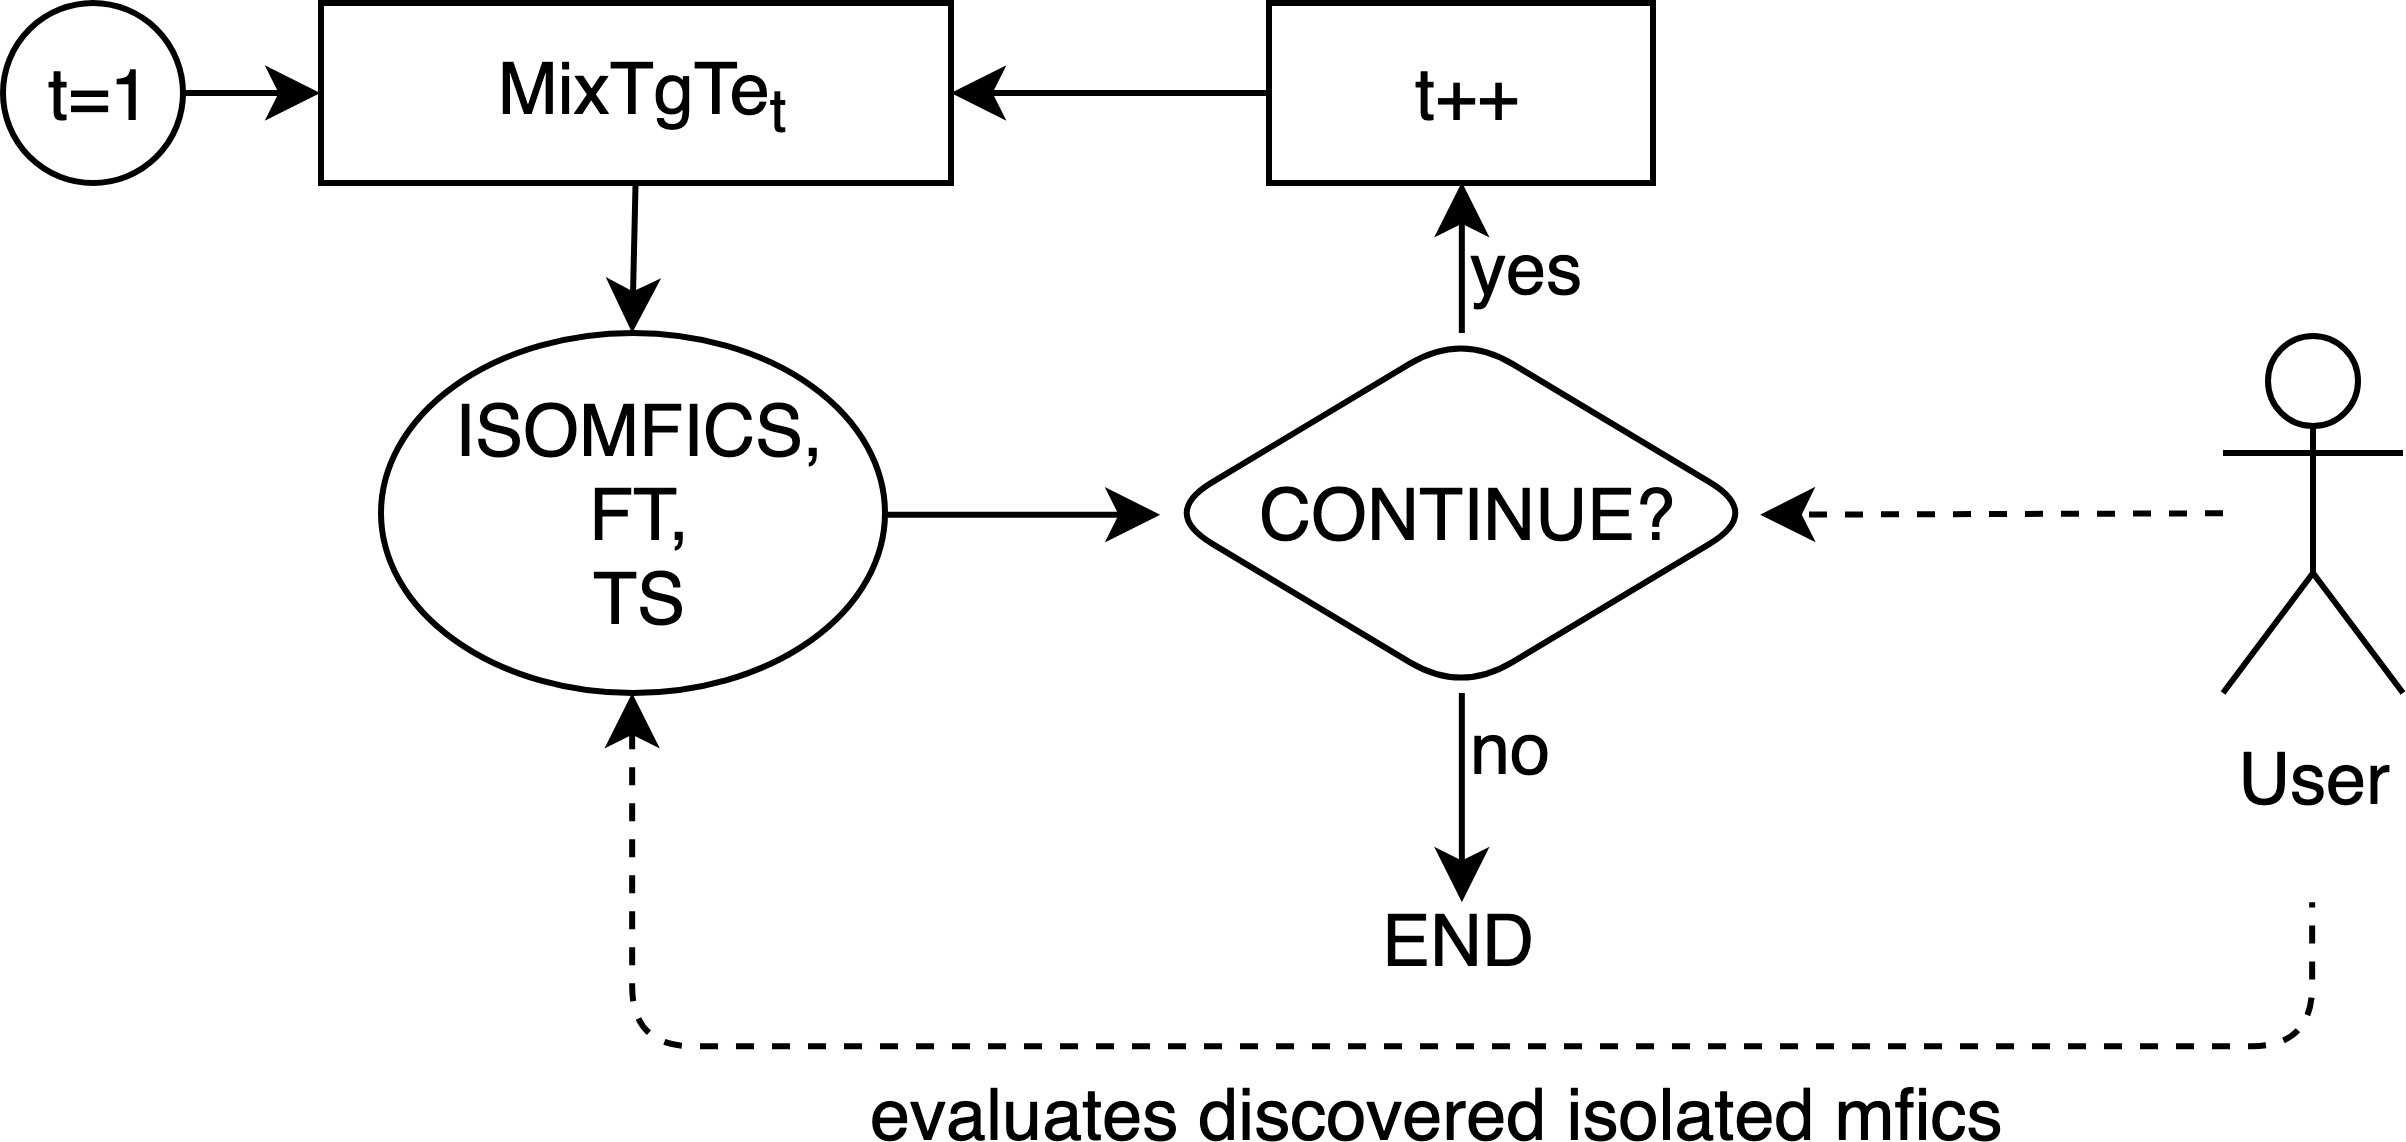
\includegraphics[width=.9\columnwidth]{images/process_mix_fl_tg}
	\caption{Overview of the user-driven iterations of the process alternating test generation and detection of isolated \mfics}
	\label{fig:overallProcess}
\end{figure}
%
\begin{algorithm}[!htb]
	\begin{algorithmic}[1]
		\State{$\isoMficsSet \gets \emptyset$}\label{line:initMFICS}
		\State{$\ft \gets \emptyset$}\label{line:initFT2}
		\State{$\ts \gets \emptyset$}\label{line:initTS}
		\State{$t \gets 1$}\label{line:initT}
		\While{$t \le \vert P \vert \wedge$ User decides to continue}
		\State{\Call{\mixt}{$t, \isoMficsSet, \ts$}}\label{line:call}
		\State{$t \gets t+1$}\label{line:increaseT}
		\EndWhile
		%\State{$mfics \gets mfics \cup \mficst$}
	\end{algorithmic}
	\caption{\mix}
	\label{alg:mix}
\end{algorithm}
%
It starts from identifying combinations of size $t$=1 using the procedure \mixt, and progressively repeats the search algorithm to combinations with higher size, until the user (who, at every iteration, can inspect the set $\isoMficsSet$ of discovered isolated \mfics of size less or equal to $t$) decides to stop the process, or $t$ reaches the number of parameters $\vert P \vert$ of the system under test. The latter condition, however, is equivalent to exercising the exhaustive test suite, and it is normally infeasible in practice, except for trivial systems.

At each step, to keep limited the number of tests to execute on the SUT, the {\it minimal} strength of the test suite used is equal to the size $t$ of the detected combinations. Indeed, by Thm.~\ref{thm:trueMficCTSt}, we can observe that this guarantees to have in the test suite all the \mfics of size $t$. However, it could be some \mfics are not isolated; therefore, at each iteration, we also generate additional tests to isolate all the discovered \mfics.

At each step, the user checks the returned sets of \isoMficsSet to determine if it is the case to continue to search for \mfics of higher strength. The choice to continue or not is based on the available budget, but may also depend on the returned \mfics in \isoMficsSet and the test suite \ts.


\end{tikzborder}
\subsection{\mixt}
\begin{tikzborder}{}	

Fig.~\ref{fig:mixTgFlT} depicts the procedure \mixt that, given a certain combination size $t$, and a set of previously executed tests, produces a combinatorial test suite of strength $t$ able to detect and isolate $\mfics$ of strength up to $t$.
%
\begin{figure}[!htb]
	\centering
	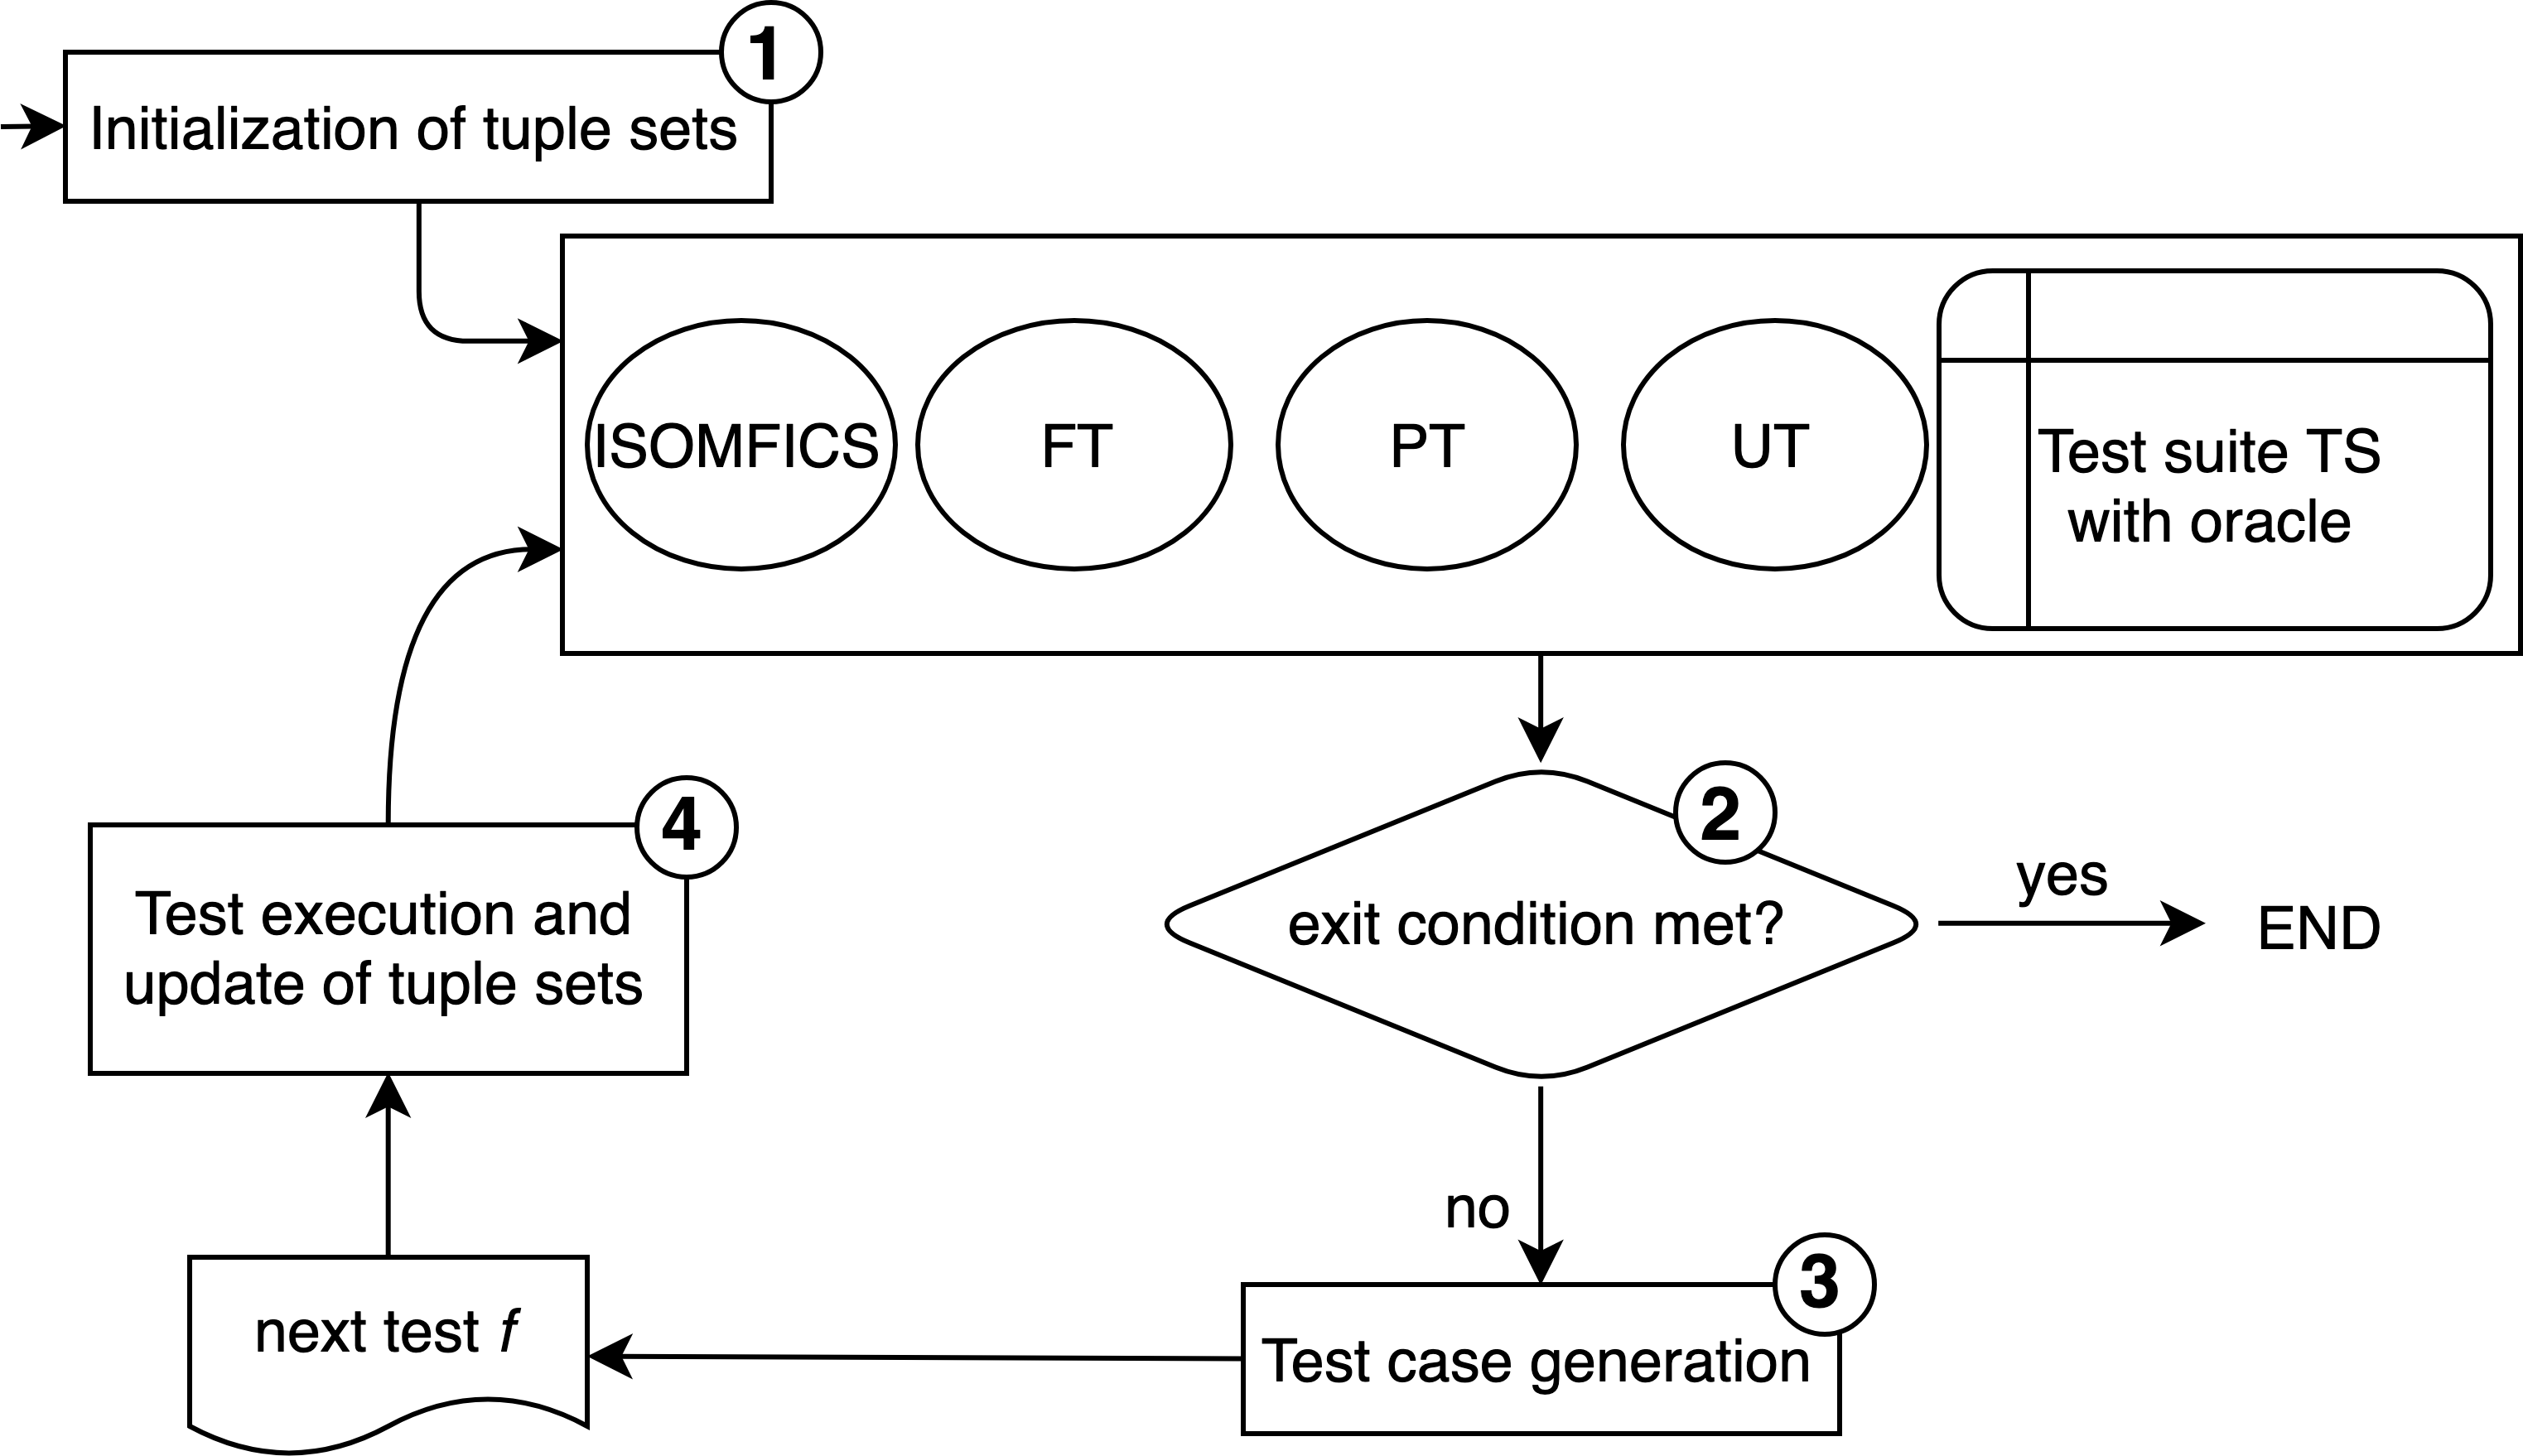
\includegraphics[width=1\columnwidth]{images/process_mix_fl_tg2}
	\caption{\mixt process to find and isolate \mfics up to accuracy of strength $t$}
	\label{fig:mixTgFlT}
\end{figure}
%
The process is described in detail in Alg.~\ref{alg:mixTgFlT} and in the rest of the section.
%
\begin{algorithm}[!htb]
	\begin{algorithmic}[1]
		\Require{$t$: strength}
		\Require{\isoMficsSet: isolated \mfics computed at step $t$-1 (empty if $t$=1)}
		\Require{\ft: failing tuples found at step $t$-1 (empty if $t$=1)}
		\Require{\ts: test suite computed at step $t$-1 (empty if $t$=1)}
		\State{$\pt \gets \{c \subseteq f | f \in \ts \wedge \resultf = \textit{pass} \wedge c \in C_t\}$}\label{line:initPT}
		\State{$\ft \gets \ft \cup \{c \subseteq f | f \in \ts \wedge \resultf = \textit{fail} \wedge c \in C_t\}\setminus \pt$}\label{line:initFT}
		\State{$\ut \gets C_t \setminus (\pt \cup \ft)$}\label{line:initUT}
		%\While{$\neg(\ut=\emptyset \wedge (\ft=\emptyset \vee (\forall c \in \ft, \exists c^\prime \in \isoMficsSet \colon c^\prime \subset c)))$}
		\While{$\neg(\ut=\emptyset \wedge (\ft=\emptyset \vee (\forall c \in \ft \colon \isExplained(c, \ts))))$}
		\State{$f \gets \mathit{buildTest}(\ut, \ft)$}
		\State{$\ts \gets \ts \cup \{f\}$}
		\State{\Call{updateTupleSets}{$f, \pt,\ft, \ut, \isoMficsSet$}}
		\State{\Call{updateMFICS}{$\ts, \ft, \isoMficsSet$}}
		\EndWhile
		%\State{$mfics \gets mfics \cup \mficst$}
	\end{algorithmic}
	\caption{\mixt}
	\label{alg:mixTgFlT}
\end{algorithm}

\mixt works on the following sets of combinations:
%
\begin{itemize}
	\item \textbf{\ut} (Unknown Tuples): the combinations of size $t$ not appeared yet in any test during the process;
	\item \textbf{\pt} (Passing Tuples): the combinations of size $\le t$ that were contained in at least one passing test executed so far in the process;
	\item \textbf{\ft} (Failing Tuples): the combinations of size $\le t$ that were contained only by failing tests, among all the tests executed so far in the process, excluding the isolated \mfics.
	\item \textbf{\isoMficsSet}: the set of isolated \mfics detected so far (of size $\le t$).
\end{itemize}
%
In addition, the process keeps track of the set of tests already run in the test suite \ts, together with the value of their \result (either pass or fail).

We give a further definition that is used in the process.

\begin{defn}[\textbf{Explained \fic}]\label{def:explainedFic}
	Given the set \isoMficsSet and a \fic $c \in \ft$, $c$ is said to be \emph{explained} if it implies one or more isolated \mfics, i.e.,
	%
	\[
	\begin{array}{l}
	\isExplained(c, \isoMficsSet) \equiv\\
	\exists S \in \mathcal{P}(\isoMficsSet) \colon c \rightarrow \bigwedge\limits_{m \in S} m
	\end{array}
	\]
\end{defn}

The rationale is that if a \fic $c$ contains\footnote{Note that, for conciseness, in the definition we use the propositional representation of tuples.} one or more \isoMfics, the failure of the tests $T_c$ in which $c$ fails can be explained. Of course, this is just a heuristic, and some other test could show that actually $c$ is the true \mfic. The definition of explained \fic will be used in the process to balance between {\it exploitation} at strength $t$ and {\it exploration} of higher strengths.
\end{tikzborder}

\subsubsection{Tuple sets initialization}

\begin{tikzborder}{}
Initially, \pt contains all the tuples of size $t$ that are contained in a passing test of \ts (line~\ref{line:initPT}); \ft, instead, inherits the failing tuples from previous iteration, and is enriched with $t$-tuples that are contained in a failing test, but not in a passing test (line~\ref{line:initFT}). \ut is initialized with the remaining tuples of size $t$ (line~\ref{line:initUT}). \isoMficsSet is kept from the previous step.
\end{tikzborder}

\subsubsection{Exit condition}\label{sec:exitCondition}

\begin{tikzborder}{}	
The process exits as soon as no unknown tuples \ut are present, and either there are no failing tuples or all the failing tuples are {\it explained} (see Def.~\ref{def:explainedFic}), i.e.,
\end{tikzborder}
%
\begin{equation}\label{eq:exitCond}
\ut = \emptyset \wedge (\ft=\emptyset \vee (\forall c \in \ft \colon \isExplained(c, \ts)))
\end{equation}

\subsubsection{Test case generation}\label{sec:testGeneration}

\begin{tikzborder}{}
If the exit condition is not met (i.e., there is at least an unknown tuple (\ut) or a failing tuple (\ft) that is not explained), the function $\mathit{buildTest}$ generates a test $f$ that contains at least one tuple belonging to either \ut, or to \ft without being explained by any subset of \mfics in \isoMficsSet. The generation works as shown in Alg.~\ref{alg:testGeneration} and described as follows:
\end{tikzborder}
%
\begin{algorithm}[!htb]
	\begin{algorithmic}[1]
		\Require{\ts: the tests generated so far}
		\Require{\ut: unknown tuples}
		\Require{\ft: failing tuples}
		\State{$f \gets \emptyset$}
		\If{$\ut \neq \emptyset$}
		\For{$c \in \ut$}\label{line:loopUt}
		\If{$\compatible(c, f)$}\label{line:compatible}
		\State{$f \gets f \cup c$}
		\EndIf
		\If{$\mathit{isCompleteTest(f)}$}
		\State \Return{$f$}
		\EndIf
		\EndFor
		\State{$f \gets \mathit{completeRnd}(f)$}\label{line:completeRnd}
		\State \Return{$f$}\label{line:returnTestUt}
		\Else
		\State{$c_{\mathit{ne}} \gets \mathit{pickRnd}(\{c \in \ft | \neg \isExplained(c, \ts)\})$}\label{line:selectUnexplained}
		\State{$\phi \gets c_{\mathit{ne}} \wedge \bigwedge_{\{f \in \ts | c_{\mathit{ne}} \subseteq f}\} \neg f$}\label{line:initPhi}
		\State{\Return$\mathtt{getModel}(\phi)$}\Comment{A test is a satisfying assignment}\label{line:satPhi}
		\EndIf
	\end{algorithmic}
	\caption{\textsc{buildTest}: Test case generation}
	\label{alg:testGeneration}
\end{algorithm}
%
\begin{tikzborder}{}
\begin{compactitem}
	\item if \ut is not empty, we merge together as many tuples $c \in \ut$ as possible (lines~\ref{line:loopUt}-\ref{line:returnTestUt}). Two tuples $c$ and $c^\prime$ cannot be merged if, for a given parameter $p_i$, $p_i$ has different values in $c$ and in $c^\prime$ (this is captured by predicate \compatible at line~\ref{line:compatible}). If after this phase some parameters have no associated value, we randomly generate values for them (line~\ref{line:completeRnd});
	\item if instead \ut is empty, we randomly select a not-explained failing tuple $c$ (line~\ref{line:selectUnexplained}); then, in lines~\ref{line:initPhi}-\ref{line:satPhi} we ask the SMT solver to find a test that contains $c$, but it is different from previous tests in \ts (this is guaranteed to exist, as shown in Thm.~\ref{thm:testGen}).
\end{compactitem}
\end{tikzborder}

\subsubsection{Test execution and tuple sets update}

\begin{tikzborder}{}
After each test $f$ is generated, it is immediately executed, and, depending on the \result (pass/fail), the tuple sets are updated as described in Alg.~\ref{alg:tupleSetsUpdate}:
\end{tikzborder}
%
\begin{algorithm}[!htb]
	\begin{algorithmic}[1]
		\Require{$f$: a test}
		\If{$\resultf$ = {\it fail}}
		\State{\Call{Move}{$f$, \ut, \ft}}
		\Else
		\State{\Call{Move}{$f$, \ut, \pt}}\label{line:moveUT}
		\State{\Call{Move}{$f$, \ft, \pt}}\label{line:moveFT}
		\State{\Call{Move}{$f$, \isoMficsSet, \pt}}\label{line:moveMfics}
		\EndIf
		
		\vspace{10pt}
		\Procedure{move}{$f$, $\sourceSet$, $\destSet$}
		\State{$\toMove \gets \{(c \in \sourceSet) | c \subseteq f\}$}
		\State{$\sourceSet \gets \sourceSet \setminus \toMove$}
		\State{$\destSet \gets \destSet \cup \toMove$}
		\EndProcedure
	\end{algorithmic}
	\caption{\textsc{updateTupleSets}: Tuple sets update}
	\label{alg:tupleSetsUpdate}
\end{algorithm}
%
\begin{tikzborder}{}
\begin{compactenum}
	\item If the test $f$ fails, all combinations that are contained both in $f$ and in the set \ut, are moved from \ut to \ft;
	\item If the test passes, we can exploit Obs.~\ref{obs:notFailureInd} and modify the sets as follows:
	\begin{compactenum}
		\item all combinations that are contained both in $f$ and in the set \ut, are moved from \ut to \pt (line~\ref{line:moveUT});
		\item all combinations that are contained both in $f$ and in the set \ft, are moved from \ft to \pt (line~\ref{line:moveFT});
		\item all combinations that are contained both in $f$ and in the set \isoMficsSet, are moved from \isoMficsSet to \pt (line~\ref{line:moveMfics}).
	\end{compactenum}
\end{compactenum}

At this point, we can evaluate whether there are new isolated \mfics, with the procedure shown in Alg.~\ref{alg:isomficsSetUpdate}.
\end{tikzborder}
%
\begin{algorithm}[!htb]
	\begin{algorithmic}[1]
		%\Procedure{updateMFICS}{}
		\Require{\ts: the tests generated so far}
		\Require{\isoMficsSet: isolated \mfics}
		\Require{\ft: failing tuples}
		
		\For{$c \in \ft$}
		\If{$\isIsoMfic(c, \ts)$}
		\State{$\ft \gets \ft \setminus \{c\}$}
		\State{$\isoMficsSet \gets \isoMficsSet \cup \{c\}$}
		\EndIf
		\EndFor
		%\EndProcedure
	\end{algorithmic}
	\caption{\textsc{updateMFICS}: \isoMficsSet set update}
	\label{alg:isomficsSetUpdate}
\end{algorithm}
%
\begin{tikzborder}{}
If a tuple $c \in \ft$ turns out to be the only one (amongst all the possible tuples) to explain the failure of a test $f$ (i.e., it is isolated in $f$ according to Def.~\ref{def:isolatedMfic}), it is added to \isoMficsSet.

In summary, the status evolution of a combination $c$ is depicted in the state machine shown in Fig.~\ref{fig:tupleLifeCycle}.
\end{tikzborder}
%
\begin{figure}[!htb]
	\centering
	\vspace{-50pt}
	\resizebox{0.6\columnwidth}{!}{
		\begin{tikzpicture}
		\tikzstyle{vertex}=[circle, minimum size=50pt,inner sep=0pt, line width=1pt, draw]
		\node[vertex, draw=none] (EMPTY) at (-1,5.1) {};
		\node[vertex, circle] (UT) at (-1,3) {\ut};
		\node[vertex, circle] (PT) at (5,3) {\pt};
		\node[vertex, circle] (FT) at (-1,0.5) {\ft};
		%\node[vertex, circle] (REM) at (-2,-2) {removed};
		\node[vertex, circle] (MFIC) at (5,0.5) {\isoMficsSet};
		\draw[->, >=latex] (EMPTY) -- (UT);
		\draw[->, >=latex] (UT) -- node[above] {pass} (PT);
		\draw[->, >=latex] (UT) -- node[right] {fail} (FT);
		\draw[->, >=latex] (FT) -- node[above] {pass} (PT);
		%\draw[->, >=latex] (PT) -- node[left] {$t$++} (REM);
		%\draw[->, >=latex] (FT) -- node[below left] {$t$++} (REM);
		\draw[->, >=latex] (MFIC) -- node[left] {pass} (PT);
		%\draw[->, >=latex] (FT) -- node[below] {\makecell{$\exists f \in \ts \colon c \subseteq f$ $\wedge \neg \result(f) \wedge$ \\ $ (\forall (c^\prime \subset f) \colon \mathit{size}(c^\prime)=t \rightarrow c^\prime \in \pt))$}} (MFIC);
		\draw[->, >=latex] (FT) -- node[below] {\makecell{$\isIsoMfic(c, \ts)$}} (MFIC);
		\end{tikzpicture}
	}
	\caption{Status evolution of a tuple $c$ throughout the process}
	\label{fig:tupleLifeCycle}
\end{figure}


\begin{example}\begin{tikzborder}{1}
	On model $M$ presented in Ex.~\ref{ex:model}, if the \truemfics were $A$ and $B\bar{C}$, a possible trace table of the process, with tests separated by the incremental maximum strength $t$, would be the one presented in Table~\ref{table:genExample} (the scenario with test 8a).
	%
\end{tikzborder}
	\begin{table*}[!htb]
		\centering
		\caption{Example of \mix for detecting $\mfics$ of different sizes with a strength up to $t=3$}
		\label{table:genExample}
		\setlength\tabcolsep{1pt}
		\vspace{2mm}
		\def\arraystretch{1.5}\tabcolsep=4pt
		\resizebox{\textwidth}{!}{%
			\begin{tabular}{c|lc|c|c||c|c|c|c|c}
				\toprule
				& \# & A & B & C & \result & \isoMficsSet & \ft & \pt & \ut \\
				\midrule
				\multirow{5}{*}{\rotatebox{90}{$t=1$}}& & \multicolumn{4}{c}{Fill FT-PT-UT} & $\{\}$ & $\{\}$ & $\{\}$ & $\{A, B, C, \bar{A}, \bar{B}, \bar{C}\}$\\ 
				\cline{2-10} 
				& 1& 0 & 0 & 0 & pass & $\{\}$ & $\{\}$ & $\{\bar{A}, \bar{B}, \bar{C}\}$ & $\{A, B, C\}$\\
				& 2 & 1 & 1 & 1 & fail & $\{\}$ & $\{A, B, C\}$ & $\{\bar{A}, \bar{B}, \bar{C}\}$ & $\{\}$\\
				& 3 & 0 & 1 & 1 & pass & $\{\}$ & $\{A\}$ & $\{\bar{A}, \bar{B}, \bar{C}, B, C\}$ & $\{\}$\\
				& \multicolumn{5}{l}{updatedMfics} & $\{A\}$ & $\{\}$ & $\{\bar{A}, \bar{B}, \bar{C}, B, C\}$ & $\{\}$\\
				\midrule
				\multirow{5}{*}{\rotatebox{90}{$t=2$}}
				& & \multicolumn{4}{c}{Fill FT-PT-UT} & $\{A\}$ & $\{AB, AC\}$ & $\{\bar{A}\bar{B}, \bar{A}\bar{C}, \bar{B}\bar{C}, \bar{A}B, \bar{A}C, BC\}$ & $\{A\bar{B}, A\bar{C}, \bar{B}C, B\bar{C}\}$\\
				\cline{2-10}
				& 4& 1 & 0 & 0 & fail & $\{A\}$ & $\{AB, AC, A\bar{B}, A\bar{C}\}$ & $\{\bar{A}\bar{B}, \bar{A}\bar{C}, \bar{B}\bar{C}, \bar{A}B, \bar{A}C, BC\}$ & $\{B\bar{C}, \bar{B}C\}$\\
				& 5 & 0 & 1 & 0 & fail & $\{A\}$ & $\{AB, AC, A\bar{B}, A\bar{C},B\bar{C}\}$ & $\{\bar{A}\bar{B}, \bar{A}\bar{C}, \bar{B}\bar{C}, \bar{A}B, \bar{A}C, BC\}$ & $\{\bar{B}C\}$\\
				& \multicolumn{5}{l}{updatedMfics} & $\{A, B\bar{C}\}$ & $\{AB, AC, A\bar{B}, A\bar{C}\}$ & $\{\bar{A}\bar{B}, \bar{A}\bar{C}, \bar{B}\bar{C}, \bar{A}B, \bar{A}C, BC\}$ & $\{\bar{B}C\}$\\
				
				& 6& 0 & 0 & 1 & pass & $\{A, B\bar{C}\}$ &$\{AB, AC, A\bar{B}, A\bar{C}\}$ & $\{\bar{A}\bar{B}, \bar{A}\bar{C}, \bar{B}\bar{C}, \bar{A}B, \bar{A}C, BC, \bar{B}C\}$ & $\{\}$\\
				
				\midrule
				\multirow{7}{*}{\rotatebox{90}{$t=3$}} %& & \multicolumn{8}{l}{Compute all 3-way tuples} \\
				& & \multicolumn{4}{c}{Fill FT-PT-UT} & $\{A, B\bar{C}\}$ &$\{AB, AC, A\bar{B}, A\bar{C}, ABC, \bar{A}B\bar{C}, A\bar{B}\bar{C}\}$ & $\{\bar{A}\bar{B}\bar{C}, \bar{A}BC, \bar{A}\bar{B}C\}$ & $\{A\bar{B}C, AB\bar{C}\}$\\
				
				\cline{2-10}
				& 7 & 1 & 0 & 1 & fail & $\{A, B\bar{C}\}$ & $\{AB, AC, A\bar{B}, A\bar{C}, A\bar{B}C, A\bar{B}\bar{C}, ABC, \bar{A}B\bar{C}\}$ & $\{\bar{A}\bar{B}\bar{C}, \bar{A}BC, \bar{A}\bar{B}C\}$ & $\{AB\bar{C}\}$\\
				
				\cline{2-10}
				& \multicolumn{6}{c}{a) Scenario in which test 8 fails} \\
				& 8a & 1 & 1 & 0 & fail & $\{A, B\bar{C}\}$ & $\{AB, AC, A\bar{B}, A\bar{C}, A\bar{B}C, A\bar{B}\bar{C}, ABC, \bar{A}B\bar{C}, AB\bar{C}\}$ & $\{\bar{A}\bar{B}\bar{C}, \bar{A}BC, \bar{A}\bar{B}C\}$ & $\{\}$\\
				
				\cline{2-10}
				& \multicolumn{6}{c}{b) Scenario in which test 8 passes} \\
				& 8b & 1 & 1 & 0 & pass & $\{\}$ & $\{A\bar{B}, AC, A\bar{B}C, A\bar{B}\bar{C}, ABC, \bar{A}B\bar{C}\}$ & $\{A, B\bar{C}, AB, A\bar{C}, \bar{A}\bar{B}\bar{C}, \bar{A}BC, \bar{A}\bar{B}C, AB\bar{C}\}$ & $\{\}$\\
				& \multicolumn{5}{l}{updatedMfics} & $\{A\bar{B}, AC, \bar{A}B\bar{C}\}$ & $\{A\bar{B}C, A\bar{B}\bar{C}, ABC \}$ & $\{A, B\bar{C}, AB, A\bar{C}, \bar{A}\bar{B}\bar{C}, \bar{A}BC, \bar{A}\bar{B}C, AB\bar{C}\}$ & $\{\}$\\
				\bottomrule
			\end{tabular}
		}
	\end{table*}
\begin{tikzborder}{}
	%
	We observe that the \truemfics have been correctly identified with the first two executions of \mixt (till test 6), i.e., tests 7 and 8a (for strength $t$=3) are not necessary, since the maximum strength of the \truemfics is 2.
	
	Instead, if the true \mfics were $A\bar{B}$, $AC$, and $\bar{A}B\bar{C}$, the process should be run three times for correctly identifying them (using test 8b), since there is a \truemfic of size 3.
\end{tikzborder}
\end{example}

\section{Properties of the \mix process}\label{sec:theorems}

\begin{tikzborder}{}	
In this section, we introduce some theorems assessing the capabilities of the proposed process.

We first make an assumption that is needed for our process.

\begin{assumption}\label{assu:oneTestEts}
	All \truemfics can be isolated.
\end{assumption}

\begin{thm}[Test case generation]\label{thm:testGen}
	In the test case generation (see Sect.~\ref{sec:testGeneration}), it is always possible to generate a test case.
\end{thm}

\begin{proof}
	When \ut is not empty, the test $f$ is generated by merging compatible tuples from \ut and then randomly selecting values for other parameters; since tuples in \ut are those that have never been observed in any test, the new test $f$ is guaranteed to exist. When \ut is empty, the generated test must be an assignment satisfying formula $\phi$ at line~\ref{line:initPhi} of Alg.~\ref{alg:testGeneration}. Let's assume that such test does not exist; it would mean that all the possible tests $T_{c_{\mathit{ne}}}$ containing $c_{\mathit{ne}}$ have already been generated; there would be two cases:
	%
	\begin{compactitem}
		\item at least one of the tests in $T_{c_{\mathit{ne}}}$ passes; this is not possible, as, in this case, $c_{\mathit{ne}}$ would be in \pt;
		\item all the tests in $T_{c_{\mathit{ne}}}$ fail; also this is not possible, as, in this case, $c_{\mathit{ne}}$ would be either in \isoMficsSet or explained by a subset of tuples in \isoMficsSet.
	\end{compactitem}
\end{proof}

\begin{thm}[Termination]\label{thm:termination}
	The process is guaranteed to terminate.
\end{thm}

\begin{proof}
	The outer process \mix terminates when the \textit{user} (i.e., the test engineer) decides not to continue it, or when $t=\vert P \vert$.
	
	The inner process \mixt terminates when the exit condition (see Eq.~\ref{eq:exitCond}) is met. The test generation phase (see Sect.~\ref{sec:testGeneration}) directly aims at emptying \ut and explaining all the not explained tuples in \ft. Since, by Thm.~\ref{thm:testGen}, the generation is always possible, the exit condition will be eventually met.
\end{proof}

We want to prove that, under the assumption that the SUT has only true \mfics of limited strength, by running the process till that strength, we will find them.

\begin{assumption}\label{assu:maxStrength}
	Each true-\mfic has maximum strength $t$.
\end{assumption}

\begin{thm}[True-\mfics found]\label{thm:trueMficsFound}
	If \trueMficsSet is the set of true \mfics and each $c$ in \trueMficsSet has maximum strength $t$, then by running the process with strength equal or greater than $t$, \isoMficsSet is equal to \trueMficsSet.
\end{thm}

\begin{proof}
	Under the stated assumption, the property is twofold: if $c$ is a \truemfic, the \mix will find it and if the \mix finds a $c$ as \mfic, then $c$ is a \truemfic.
	%
	\begin{compactenum}
		\item If $c$ is a \truemfic then \isoMficsSet will contain $c$. Let's assume that $c$ is a \truemfic but \isoMficsSet does not contain it at the end. By Thm.~\ref{thm:trueMficCTSt}, $c$ is contained in a failing test of \ts and so it is in \ft at a given point. When the process terminates, \ft is either empty (and so $c$ is in \isoMficsSet), or all the tuples in \ft are explained (by Def.~\ref{def:explainedFic}), i.e., they contain one or more \isoMfic. However, the latter case is not possible, as $c$ would not be minimal.
		\item If $c$ is in \isoMficsSet, it is a \truemfic. Let's assume that $c$ is in \isoMficsSet, but it's not a \truemfic. If $c$ is in \isoMficsSet, all tests containing it fail, and there exists a test in which it is the only \mfic; if it is not a \truemfic, it means that in each test containing $c$ there must be a combination $c^\prime$ such that $c \subset c^\prime$ and $c^\prime$ is a \truemfic and, therefore, added to \isoMficsSet by point 1: in this case, $c^\prime$ would violate the minimality requirement. Note that, if $c$ has size $t$, there cannot be a \truemfic $c^\prime$ of higher strength containing $c$ by Assumption~\ref{assu:maxStrength}.
	\end{compactenum}
\end{proof}
\end{tikzborder}

\section{Evaluation}\label{sec:evaluation3}

\begin{tikzborder}{}
In this section, we evaluate the process and we compare it with other techniques for fault interaction detection.
\end{tikzborder}

\subsection{Benchmarks}\label{sec:benchmarks}

\begin{tikzborder}{}
For the experiments, we selected some benchmarks, each one constituted by a faulty version of the SUT $S_f$ and an oracle $O$. The assessment of the execution of a test $f$ (i.e., \result in Def.~\ref{def:testCase}) is performed by comparing the evaluations of $f$ over $S_f$ and $O$. For practicality, we build a combinatorial model $M$ having the same parameters of $S_f$\footnote{Note that $S_f$ and $O$ have the same parameters and they only differ on the behaviour.} and constraints that accept only the tests for which $S_f$ and $O$ agree (the constraints are the negation of the \truemfics).\footnote{Note that these constraints are not related to the combinatorial problem that, as stated in Sect.~\ref{sec:background}, is unconstrained in our setting.} Therefore, for each benchmark, we also know the \truemfics in $S_f$.

We used two sets of benchmarks described in Table~\ref{table:benchmarks}.
\end{tikzborder}
%
\begin{table}[!htb]
	\centering
	\caption{Benchmark properties}
	\label{table:benchmarks}
	%\resizebox{\columnwidth}{!}{%
	%\setlength\tabcolsep{1pt}
	\begin{tabular}{c|cccr} 
		\toprule
		& name & $\vert P \vert$ & size & \trueMficsSet\\
		& & & & \multicolumn{1}{c}{(size (\#))}\\
		\midrule
		\multirow{8}*{\rotatebox{90}{\small \benchArt}}
		&{\tt runExA} & 3 & $2^3$ & 1(1), {\bf 2}(1)\\
		&{\tt runExB} & 3 & $2^3$ & 2(2), {\bf 3}(1)\\
		&{\tt art1} & 3 & $2^3$ & {\bf 2}(1)\\
		&{\tt art2} & 3 & $2^3$ & {\bf 2}(2)\\
		&{\tt art3} & 3 & $2^3$ & 1(1), {\bf 2}(1)\\
		&{\tt art4} & 7 & $2^7$ & 2(1), {\bf 3}(1)\\
		&{\tt art5} & 7 & $2^7$ & {\bf 2}(1)\\
		&{\tt art6} & 5 & $2^3 3^1 5^1$ & {\bf 3}(1) \\
		%& {\tt Django} & 24 & $2^{23} 4^1$ & $1^2 2^2$ \\
		\midrule
		\multirow{5}*{\rotatebox{90}{\small \benchReal}}
		& {\tt aircraft} & 8 & $2^7 3^1$ & 3(1), {\bf 4}(1)\\
		& {\tt tomcat} & 12 & $2^8 3^1 4^1$ & 1(1), {\bf 2}(2)\\
		& {\tt hsqldb} & 10 & $2^9 6^1$ & 1(1), {\bf 3}(2)\\
		& {\tt gcc} & 10 & $2^8 3^1 4^1 $ & {\bf 3}(4)\\
		& {\tt jflex} & 13 & $2^{10} 3^2 4^1 $ & {\bf 2}(1)\\
		\bottomrule
	\end{tabular}
	%}
\end{table}
%
\begin{tikzborder}{}
The first benchmark set, \benchArt, is constituted by \textit{artificial} models of systems; we generated some of these models with one \truemfic (\texttt{art1}, \texttt{art5}, and \texttt{art6}), and others with multiple \truemfics. \benchArt also contains the running example, in its two versions shown in Table~\ref{table:genExample}. The second benchmark set, \benchReal, represents real systems: \texttt{aircraft} is a Software Product Line model presented in~\cite{Voelter:2009} and taken from the SPLOT repository\footnote{http://www.splot-research.org/}, and the others four are benchmarks used in Niu et al.~\cite{Niu2018interleaving}.

In Table~\ref{table:benchmarks}, column \textit{size} reports the size of model $M$, presented in the abbreviated form $k^{\# \mathit{params}_k} \times \ldots$, where $k$$\in$$N^+$ and $\mathit{params}_k$ are the parameters having $k$ values; for example, $2^8$$3^1$$4^1$ indicates that the SUT has 8 parameters that can take 2 values, one parameter taking 3 values, and one parameter taking 4 values. Column \trueMficsSet reports the number and size of \truemfics in $M_f$; we report each possible size with the number of \mfics of that size in parentheses. We also mark in bold face the maximum strength of the \truemfic; in the experiments, we assume Assumption~\ref{assu:maxStrength}, and so we apply the approach only up to the known maximal strength (according to Thm.~\ref{thm:trueMficsFound}, this guarantees to find all the \mfics).
\end{tikzborder}

\subsection{Compared approaches}\label{sec:processes}

\begin{tikzborder}{}
We compare our approach with some existing methods from literature, namely:
%
\begin{asparadesc}
	\item[BEN:] a process based on the first phase of the BEN tool proposed by Ghandehari et al.~\cite{ben_2015}. The process consists in calling BEN for failure-inducing combination detection, by providing an initial combinatorial test suite of a certain strength $t$, and iterating over the size of the failure-inducing combinations to try to detect them. This process has already been used for constraints validation and repair~\cite{Gargantini16:validation,gargantini_combinatorial_2017}. The BEN tool is included in our experimental process as a jar file.
	\item[SOFOT:] the \textit{Simplified One Factor One Time} method to infer the Minimal Failure-causing Schema (\textsf{MFS}) from a given failing test case, from Nie et al.~\cite{nie_2011}. This method takes as input a set of failing tests, and tries to reduce each test to an \mfic. For each failing test $f$, it generates new tests by changing the value of each parameter in $f$ one by one. Note that the source code of this method is available in Python from a later work by Zhang and Zhang~\cite{zhang_characterizing_2011}. As our automated evaluation script is written in Java, we program it so that it calls Python via command line. This causes some overhead which affects the total execution time in the experiments.
	\item[FIC:] the \textit{Faulty Interaction Characterization} method proposed by Zhang et al.~\cite{zhang_characterizing_2011}. It is similar to SOFOT, in the sense that it accepts in input a set of tests known to be failing, and it tries to isolate the minimal failure-inducing combination(s) from it. It proceeds by considering one failing test a time, and changing the value of a parameter at a time, but, unlike SOFOT, it keeps the value changed. Furthermore, it performs a few iterations until the original failing test, with the value of the detected minimal failure-inducing combinations changed, passes. If there are two different failure-inducing combinations in the same tests, it may find them, but without a guarantee to be correct. We made a Java implementation of the algorithm described in the paper~\cite{zhang_characterizing_2011}.
	\item[ICT:] the \textit{Interleaving CT} approach proposed by Niu et al.~\cite{Niu2018interleaving}. It is a significant improvement of SOFOT that alleviates its three main problems: redundant test cases, multiple \mfics, and masking effects (where multiple \mfics are present in the same test). Like SOFOT, it is composed of two phases, generation and identification. Test generation is here made adaptive, one test at a time, in a similar way as the one of our approach. This reduces the amount of tests needed, by forbidding the generation of new tests containing already discovered failure-inducing combinations. The identification phase has a novel feedback checking mechanism (based on information coming from the execution of a few new proposed test cases), which can check, up to a certain extent, whether the identified \mfic is a \truemfic or not; and it significantly improves the accuracy of the results w.r.t. SOFOT. The method is very recent, and, although we could not manage to re-run the tool on new benchmarks, we compared the results of \mix with the results of ICT reported in that paper for a common set of benchmarks.
\end{asparadesc}

Since FIC and SOFOT require failing tests as input, but do not say how to find such failing tests, we need to build a test suite to find such failing tests. In order to try to make the comparison fair, we use, for all the methods\footnote{Note that \mix, BEN, and ICT already require a combinatorial test suite.}, an initial combinatorial test suite $\cts_t$ of strength $t$=$\max\limits_{c \in \trueMficsSet}|\mathit{size}(c)|$, being \trueMficsSet the set of \truemfics (as shown in Table~\ref{table:benchmarks}). 
$\cts_t$ is generated using ACTS\footnote{https://csrc.nist.gov/projects/automated-combinatorial-testing-for-software} for FIC, BEN, and SOFOT. \mix, instead, generates tests in an adaptive way, as described in Sect.~\ref{sec:testGeneration}. ICT, instead, uses AETG~\cite{AETG}.

In the following, \detMficsSet denotes the set of \mfics returned by a method; in our case, it corresponds to \isoMficsSet.
\end{tikzborder}

\subsection{Results}\label{sec:results}

\begin{tikzborder}{}
We run our method and the compared 4 methods 10 times for each benchmark; results are the average across the runs. Experiments have been executed on a Mac OS X 10.14, Intel Core i3, with 4GB of RAM. Code was written in Java, using CTWedge libraries for combinatorial modeling, test generation, and test execution~\cite{IWCTGargantini2018}. The code and all the benchmarks are available online at https://github.com/fmselab/mixtgte.

Table~\ref{table:resultsByBenchmarkPrecRec} shows the results of the experiments.
\end{tikzborder}
%
\begin{table*}[!htb]
	\centering
	\caption{Experimental results (P: precision, R: recall, F: F-score, time is in ms)}
	\label{table:resultsByBenchmarkPrecRec}
	\resizebox{\columnwidth}{!}{%
	\setlength\tabcolsep{2.1pt}
	\begin{tabular}{c|c|ccccr|ccccr|ccccr|ccccr|ccccr} 
		\toprule
		& model & \multicolumn{5}{c}{$\mix$} & \multicolumn{5}{c}{FIC} & \multicolumn{5}{c}{BEN} & \multicolumn{5}{c}{SOFOT} & \multicolumn{5}{c}{ICT}\\
		& & tests & P & R & F & time & tests & P & R & F & time & tests & P & R & F & time & tests & P & R & F & time & tests & P & R & F & time \\
		\midrule
		\multirow{8}*{\rotatebox{90}{\small \benchArt}}
		&{\tt runExA} & 7.6 & 1 & 1 & 1 & 15.9 & 8 & 1.00 & 1.00 & 1.00 & 0.4 & 7 & 0.20 & 0.50 & 0.29 & 53.2 & 8 & 0.75 & 0.50 & 0.58 & 518 & -- & -- & -- & -- & --\\
		&{\tt runExB} & 8.0 & 1 & 1 & 1 & 4.9 & 8 & 0.75 & 1.00 & 0.86 & 0.6 & 8 & 0.25 & 0.33 & 0.29 & 9.4 & 8 & 0.75 & 1.00 & 0.86 & 735 & -- & -- & -- & -- & --\\
		&{\tt art1} & 6.6 & 1 & 1 & 1 & 3.2 & 5 & 1.00 & 1.00 & 1.00 & 0.5 & 7 & 1.00 & 1.00 & 1.00 & 13.0 & 7 & 1.00 & 1.00 & 1.00 & 269 & -- & -- & -- & -- & --\\
		&{\tt art2} & 8.0 & 1 & 1 & 1 & 5.4 & 7 & 1.00 & 1.00 & 1.00 & 0.6 & 7 & 0.50 & 0.50 & 0.50 & 13.8 & 8 & 0.50 & 0.50 & 0.50 & 396 & -- & -- & -- & -- & -- \\
		&{\tt art3} & 7.6 & 1 & 1 & 1 & 2.7 & 8 & 1.00 & 1.00 & 1.00 & 0.7 & 7 & 0.00 & 0.00 & -- & 15.1 & 8 & 1.00 & 0.50 & 0.67 & 403 & -- & -- & -- & -- & --\\
		&{\tt art4} & 36.9 & 1 & 1 & 1 & 79.7 & 29 & 0.67 & 1.00 & 0.80 & 1.8 & 26 & 0.00 & 0.00 & -- & 64.8 & 61 & 1.00 & 1.00 & 1.00 & 2772 & -- & -- & -- & -- & --\\
		&{\tt art5} & 14.7 & 1 & 1 & 1 & 5.0 & 12 & 1.00 & 1.00 & 1.00 & 0.5 & 18 & 1.00 & 1.00 & 1.00 & 14.1 & 20 & 1.00 & 1.00 & 1.00 & 769 & -- & -- & -- & -- & --\\
		&{\tt art6} & 45.4 & 1 & 1 & 1 & 17.1 & 35 & 0.50 & 1.00 & 0.67 & 3.2 & 38 & 1.00 & 1.00 & 1.00 & 21.1 & 52 & 1.00 & 1.00 & 1.00 & 1830 & -- & -- & -- & -- & --\\
		\midrule
		\multirow{5}*{\rotatebox{90}{\small \benchReal}}
		& {\tt aircraft} & 89.8 & 1 & 1 & 1 & 156.5 & 71 & 1.00 & 1.00 & 1.00 & 18.4 & 62 & 0.00 & 0.00 & -- & 56.4 & 115 & 1.00 & 1.00 & 1.00 & 4157 & -- & -- & -- & -- & --\\
		& {\tt gcc} & 88.5 & 1 & 1 & 1 & 134.5 & 64 & 0.50 & 0.50 & 0.50 & 8.9 & 60 & 1.00 & 0.50 & 0.67 & 56.1 & 142 & 0.75 & 0.75 & 0.75 & 4934 & 89.0 & 0.77 & 0.65 & 0.70 & 1118 \\
		&{\tt hsqldb} &169.8 & 1 & 1 & 1 & 3752.8 & 97 & 1.00 & 1.00 & 1.00 & 36.6 & 55 & 0.00 & 0.00 & -- & 532.2 & 443 & 1.00 & 0.67 & 0.80 & 19612 & 88.3 & 1.00 & 1.00 & 1.00 & 2094 \\
		&{\tt jflex} & 22.9 & 1 & 1 & 1 & 9.1 & 15 & 1.00 & 1.00 & 1.00 & 1.6 & 23 & 1.00 & 1.00 & 1.00 & 15.2 & 31 & 1.00 & 1.00 & 1.00 & 978 & 31.6 & 1.00 & 1.00 & 1.00 & 187 \\
		&{\tt tomcat} & 65.9 & 1 & 1 & 1 & 111.9 & 28 & 0.67 & 0.67 & 0.67 & 4.1 & 23 & 0.00 & 0.00 & -- & 31.5 & 128 & 1.00 & 1.00 & 1.00 & 5675 & 128 & 1.00 & 1.00 & 1.00 & 5671 \\
		%& {\tt Connector} & 20 & 20 \\
		\midrule
		& Average & 44.0 & 1 & 1 & 1 & 331 & 29.8 & 0.85 & 0.94 & 0.88 & 5.99 & 26.2 & 0.46 & 0.45 & 0.44 & 68.9 & 79.3 & 0.90 & 0.84 & 0.86 & 3311 & 67.4 & 0.94 & 0.91 & 0.92 & 988 \\
		\bottomrule
	\end{tabular}
	}
\end{table*}
%
\begin{tikzborder}{}
For each method, it reports the total number of different tests required to complete the detection\footnote{If a test is generated twice by a method, we count it only once.}, and the execution time in milliseconds. Moreover, in order to measure the {\it quality} of the returned \mfics, we use classical measures as {\it precision} (P), {\it recall} (R), and {\it F-score} (F). Precision is defined as:
%
\[\mathit{precision} = \frac{|\detMficsSet \cap \trueMficsSet|}{|\detMficsSet|}\]
%
Precision measures the percentage of found \mfics that are \truemfics. If precision is not 1, the developer will spend some time in doing fault localization for a \fic that is not a \truemfic (those in $\detMficsSet \setminus\trueMficsSet$).

Recall is defined as:
%
\[\mathit{recall} = \frac{|\detMficsSet \cap \trueMficsSet|}{|\trueMficsSet|}\]
%
It measures how many \truemfics are actually identified. If the recall is not 1, the developer is not aware of a \truemfic that causes a fault (those in $\trueMficsSet \setminus \detMficsSet$).

The F-measure is the combination of precision and recall, defined as follows:
%
\[\textnormal{\it F-score} = \frac{2 \times \mathit{precision} \times \mathit{recall}}{\mathit{precision} + \mathit{recall}}\]

We now evaluate the approach answering the following three research questions.

\researchquestion{How is the effectiveness (in terms of precision and recall) of \mix w.r.t. other techniques?}

From the results presented in Table~\ref{table:resultsByBenchmarkPrecRec}, we observe that \mix always achieves maximum precision and recall; this is expected, as Thm.~\ref{thm:trueMficsFound} guarantees that, under the assumption that we know the maximum strength $t$, executing \mix till strength $t$ produces an \isoMficsSet set (i.e., \detMficsSet) equal to \trueMficsSet. All the other techniques do not provide this theoretical guarantee.

Among the other methods, ICT has the highest values for precision, recall, and \fScore (92\% on average) on the 4 available benchmarks~\cite{Niu2018interleaving}. For 3 benchmarks, ICT correctly identified all the \trueMficsSet; only for \textit{gcc}, some are wrongly identified (precision 77\%) and some are not found (recall 65\%).

Also FIC and SOFOT showed to be able to correctly identify the \truemfics in many occasions, although not with the same overall accuracy as ICT in terms of \fScore (88\% and 86\%). We believe that this is due not only to the fixed amount of tests asked for the \textit{identification} phase of those methods (they change always one parameter at a time, and only once), but also to the \textit{masking effect}, i.e., when there are two \mfics present in a same test. This effect may happen in general, as explained in Thm.~\ref{thm:insufficientAccuracyCTSt}. As an example of this fact, consider the running example described in Ex.~\ref{ex:model} and the test suite generated by SOFOT shown in Table~\ref{table:executionSOFOT}.
%
\begin{table}[!htb]
	\centering
	\caption{Execution trace of SOFOT on example SUT}
	\label{table:executionSOFOT}
	%\resizebox{.8\columnwidth}{!}{%
	\footnotesize
	\begin{tabular}{r|c|c|c||c}
		\multicolumn{5}{c}{Generation of $\cts_2$ with ACTS (to have some failing test)}\\
		\toprule
		%\multicolumn{5}{c}{2-way combinatorial coverage to find the faults} \\
		%\midrule
		\# & A & B & C & \result \\
		\hline 
		%& \multicolumn{4}{c}{1-way combinatorial coverage to find the faults} \\
		%1& 1 & 0 & 0 & \textsf{pass} \\
		%2& 0 & 1 & 1 & \textsf{pass} \\
		%\hline
		%1& 1 & 1 & 0 & \textsf{fail} $\vartriangleleft$ fault \ding{172} detected\\
		1& 1 & 1 & 0 & failing test \ding{172}\\
		%2& 1 & 0 & 1 & \textsf{fail} $\vartriangleleft$ fault \ding{173} detected\\
		2& 1 & 0 & 1 & failing test \ding{173}\\
		3& 0 & 1 & 1 & \textsf{pass} \\
		4& 0 & 0 & 0 & \textsf{pass} \\
		\bottomrule
		\multicolumn{5}{c}{}\\
		\multicolumn{5}{c}{}\\ 
		\multicolumn{5}{c}{Identification by SOFOT (tests added to find \mfics)} \\
		\toprule
		\multicolumn{5}{c}{additional tests for failing test \ding{172}} \\
		\midrule
		\# & A & B & C & \result \\
		\hline
		5& 0 & 1 & 0 & \textsf{fail} \\
		6& 1 & 0 & 0 & \textsf{fail} \\
		7& 1 & 1 & 1 & \textsf{fail} \\
		\multicolumn{5}{c}{No \mfic found}\\ 
		\hline
		\multicolumn{5}{c}{} \\
		\hline
		\multicolumn{5}{c}{additional tests for failing test \ding{173}}\\
		\midrule
		\# & A & B & C & \result \\
		\hline
		8& 0 & 0 & 1 & \textsf{pass} \\
		--& 1 & 1 & 1 & \textsf{fail} \\
		--& 1 & 0 & 0 & \textsf{fail} \\
		\multicolumn{5}{c}{$A$ identified as \mfic}\\ 
		\bottomrule
	\end{tabular}
	%}
\end{table}
%
Let's recall that the SUT is made of three binary parameters \{A, B, C\}, with two \truemfics, $A$ and $B\bar{C}$. By providing to SOFOT the faulty test cases observed with a combinatorial test suite of strength $t=2$ (that it is also the maximum strength of the \truemfics, so the correct settings for the experiments) generated with ACTS, the SOFOT method is able to correctly identify only the \mfic $A$. Table~\ref{table:executionSOFOT} reports, at the beginning, the $\cts_2$ generated by ACTS; it contains two failing tests for which SOFOT tries to find the \mfic.
In test \ding{172}, both \truemfics $A$ and $B\bar{C}$ are contained; all the additional tests generated by SOFOT for this test (obtained by changing one parameter at a time) fail. Therefore, for test \ding{172}, SOFOT does not find any \mfic, i.e., it does not find $A$ nor $B\bar{C}$. This is due to the masking effect in test \ding{172} between $A$ and $B\bar{C}$. The tests generated for the failing test \ding{173}, instead, correctly identifies $A$ as \mfic.

BEN is the method with the lowest \fScore; this is because BEN is configured to produce few additional tests and uses heuristics to measure the suspiciousness of a failing tuple, and this may lead to wrong results.

\researchquestion{How does our approach compare with the others in terms of number of tests?}

Overall, the number of tests required by \mix is comparable to ICT. On the four real benchmarks in common, \mix requires slightly fewer tests for \texttt{gcc} and \texttt{jflex}, but more tests for the other two benchmarks. For \texttt{hsqldb}, \mix requires almost the double of the tests. This is due to the fact that ICT applies efficient heuristics to limit the number of tests that are asked in addition to the initial combinatorial test suite; \mix, instead, does not have such strong optimizations, that we plan to investigate as future work. For this particular benchmark \texttt{hsqldb}, ICT is better (or equal) than our approach on any aspect (it also achieves 100\% F-score); however, it does not provide any particular correctness guarantee.

SOFOT requires the highest amount of tests, and it obtains a lower recall, but a higher precision than FIC. The other two analyzed methods (FIC and BEN) require fewer tests (almost half of the test of \mix on average), but, as described in {\bf RQ1}, they also achieve less precision and recall than both \mix and ICT.

\researchquestion{How does our approach compare with the others in terms of time?}

All the reported times (for all the approaches) do not include the time for actually exercising the real system to determine the \result (pass/fail) of the test. Indeed, the real system has been mocked by a model, since we know the \truemfics beforehand.

We cannot directly compare the execution time of ICT and SOFOT. Indeed, we were not able to rerun ICT on our machine (we report the results of the original paper~\cite{Niu2018interleaving}). For SOFOT, instead, we need to perform calls to an external Python program from Java, that introduce a big overhead.

The execution time for our process varies a lot depending on the number of generated tests, and the maximum strength achieved. It is less than 20ms for more than half of the benchmarks; however, it takes around 3.8 secs for \texttt{hsqldb}, which has two \truemfics of size 3, and one of size 1. The \mfic of size 1 causes several tests to fail, masking the effect of the 3-way \mfics. Note that, although \texttt{gcc} has four 3-way \truemfics, it takes less computation time because less tests are needed to isolate the \mfics from the other failing tuples, as more tests are passing.

Generally, BEN is quite fast as it does not produce too many tests, and the time is not affected too much by the model size; in our case, instead, time is more dependent on the benchmark characteristics (model size, number of \truemfics, presence of masking effect, etc.).

FIC is the fastest method, as it only requires, on average, around 6ms per benchmark, with a maximum time of 36.6ms for \texttt{hsqldb}.

\end{tikzborder}
\section{Related Work}\label{sec:related}
\begin{tikzborder}{}	

Identifying the real failure inducing combinations is an area of active research in combinatorial testing~\cite{nie_2011, kuhn_practical_2010}.

Previous works in detecting failure-inducing interactions are based on post-analysis of the test results of covering arrays (CAs), or on adaptive or non-adaptive test generation techniques. Yilmaz et al.~\cite{CohenTSE06} applied a post-analysis classification tree technique to analyze the result of CAs to find the differences between passing and failing tests. However, CA is not suitable to detect \mfics precisely. Among non-adaptive methods, there is an approach based on pseudo-Boolean constraint solving and optimization, but its accuracy is highly affected by the chosen test suite~\cite{Zhang2012FII}.
Locating and detecting arrays (LDAs)~\cite{colbourn_locating_2008}, 
and error locating arrays (ELAs)~\cite{martinez_locating_2010} are other non-adaptive approaches: they require a given strength $t$ and a maximum number of faulty interactions $d$, and they can detect and locate at most $d$ faulty interactions of size up to $t$. However, the size of the test suite often becomes very large. That is why, recently, adaptive methods appear to be more studied in literature. They include Wang's IterAIFL method~\cite{wang_adaptive_2010}, which is based on AIFL by Shi et al.~\cite{shi_software_nodate}, two adaptive algorithms proposed by Martinez et al.~\cite{martinez_locating_2010}, and all the methods used to compare our process in the experiments: FIC (and also the variant FIC\_BS) by Zhang et al.~\cite{zhang_characterizing_2011}, BEN~\cite{ghandehari2018combinatorial}, SOFOT~\cite{nie_2011}, and ICT~\cite{Niu2018interleaving}.

While InterAIFL, FIC and SOFOT may not correctly identify multiple \mfics in a system, since they may be overlapping or there is a masking effect, the two adaptive algorithms of Martinez work better but they can only locate \mfics up to size 2. The ICT approach by Niu et al.~\cite{Niu2018interleaving}, still derived from SOFOT, overcomes its limitations, making a significant improvement in the accuracy of the detected combinations. BEN~\cite{ghandehari2018combinatorial} is tailored to locate faults in the code, but in the first phase it provides an algorithm to detect \textit{suspicious} combinations and, with some heuristics, \textit{failure-inducing} combinations. However, as implemented so far, it is not very accurate with the initial test suites provided as input: an initial test suite of higher strength could improve accuracy of the detected \mfics. Unlike the other methods, \mix does not distinguish between the two phases of the input test generation and additional adaptive test, but it merges those phases into one single process, that keeps track of the status of all the possible t-way tuples throughout the process. This way, \mix has shown to correctly detect all the \mfics of a system, up to a certain strength $t$ decided by the user, and it guarantees them to be correct under the assumption that there are no faults caused by an interaction of strength higher than $t$.

%\red{da citare \cite{Zhang2012FII}}

\end{tikzborder}

\bookmarksetup{startatroot}
\chapter{Conclusions}\
We illustrated the research project of using software testing techniques to drive the inference and repair of models of software systems.
It is a novel application of software testing that goes beyond detecting and localizing faults in code, and that performs little repairs to preserves domain knowledge and support engineers in maintaining consistency between all the software artifacts, and localizing faults also in the model. 
We presented applications to combinatorial and feature models. As future work, we plan to apply test-driven repair of other model types, namely timed automata, and abstract state machines. Furthermore, we plan to improve the process of combinatorial models repair by improving the accuracy of the fault localization strategy.

\section{Future Work}
TODO: apply the repair process to more kind of models, if necessary through an abstraction and parametrization process (as in Timed Automata, see Chapter. \ref{ch:tarepair}).
Improve each paper by doing what described as future work.
Although these contributions have also been implemented, the program is tailored towards producing experiments table on the benchmarks proposed in the paper, and an easy-to-use tool publicly available could further promote the usage of the finding of our research. 
In some cases the process is not fully automated, manual intervention (even if just to move, rename some files, or translate language formats) for certain tasks is needed (especially for timed automata repair, and for xss detection), so make a tool out of it, although expensive, would promote the usage of the devised processes.

%\chapter{Bibliography}
\addcontentsline{toc}{chapter}{Bibliography}
 

%----------------------------------------------------------------------------------------
%	THESIS CONTENT - APPENDICES
%----------------------------------------------------------------------------------------

%\appendix % Cue to tell LaTeX that the following "chapters" are Appendices

% Include the appendices of the thesis as separate files from the Appendices folder
% Uncomment the lines as you write the Appendices

%% Appendix A

\chapter{Frequently Asked Questions} % Main appendix title

\label{AppendixA} % For referencing this appendix elsewhere, use \ref{AppendixA}

\section{How do I change the colors of links?}

The color of links can be changed to your liking using:

{\small\verb!\hypersetup{urlcolor=red}!}, or

{\small\verb!\hypersetup{citecolor=green}!}, or

{\small\verb!\hypersetup{allcolor=blue}!}.

\noindent If you want to completely hide the links, you can use:

{\small\verb!\hypersetup{allcolors=.}!}, or even better: 

{\small\verb!\hypersetup{hidelinks}!}.

\noindent If you want to have obvious links in the PDF but not the printed text, use:

{\small\verb!\hypersetup{colorlinks=false}!}.

%\include{Appendices/AppendixB}
%\include{Appendices/AppendixC}

%----------------------------------------------------------------------------------------
%	BIBLIOGRAPHY
%----------------------------------------------------------------------------------------

%\printbibliography[heading=bibintoc,title=Bibliography]
%\bibliographystyle{plain}
\bibliography{thesis}
%\bibliographystyle{ieeetr}
%----------------------------------------------------------------------------------------

\end{document}  
